%%%%%%%%%%%%%%%%%%%%%%%%%%%%%%%%%%%%%%%%%%%%%%%%%%%%%%%%%%%%%%%%%%%%%%
%%  disstemplate.tex, to be compiled with latex.                     %
%%  08 April 112002     Version 4                                    %
%%%%%%%%%%%%%%%%%%%%%%%%%%%%%%%%%%%%%%%%%%%%%%%%%%%%%%%%%%%%%%%%%%%%%%
%%                                                                   %
%%  Writing a Doctoral Dissertation with LaTeX at                    %
%%      the University of Texas at Austin                            %
%%                                                                   %
%%  (Modify this ``template'' for your own dissertation.)            %
%%                                                                   %
%%%%%%%%%%%%%%%%%%%%%%%%%%%%%%%%%%%%%%%%%%%%%%%%%%%%%%%%%%%%%%%%%%%%%%

\PassOptionsToPackage{pagebackref=true}{hyperref} % Ensure pagebackref used
\documentclass[final,letterpaper,12pt]{report}    % Must be 'report' class

\usepackage{utdiss2}               % Dissertation package style file


%%%%%%%%%%%%%%%%%%%%%%%%%%%%%%%%%%%%%%%%%%%%%%%%%%%%%%%%%%%%%%%%%%%%%%
% Optional packages used for this sample dissertation. If you don't  %
% need a capability in your dissertation, feel free to comment out   %
% the package usage command.                                         %
%%%%%%%%%%%%%%%%%%%%%%%%%%%%%%%%%%%%%%%%%%%%%%%%%%%%%%%%%%%%%%%%%%%%%%
% Fonts per http://www.khirevich.com/latex/font/
% Can drop charter/mathdesign and use amsfonts,amssymb if problematic
% Will likely need to add package mathrsfs if that is done
\usepackage[T1]{fontenc}
\usepackage[charter]{mathdesign}
\usepackage{amsmath,amsthm}
\usepackage[usenames,dvipsnames,svgnames,table]{xcolor}
\usepackage{color}

\usepackage{accents}
\usepackage{afterpage}
\usepackage{array}
\usepackage{bookmark}
\usepackage{booktabs}
\usepackage[english]{babel}
\usepackage{blindtext}
\usepackage{bm}
\usepackage{calc}
\usepackage{caption}
\usepackage{enumitem}
\usepackage{floatpag}
\usepackage{helvet}
\usepackage[final]{graphicx} % "final" causes images to appear in draft mode
\usepackage{ifdraft}
\usepackage{ifthen}
\usepackage[final]{listings}
\usepackage{longtable}
\usepackage{makecell}
\usepackage[warn]{makecmds}
\usepackage{mathtools}
\usepackage{multirow}
\usepackage{multicol}
\usepackage[numbers,sort&compress]{natbib}
\usepackage{nicefrac}
\usepackage{pgfplotstable}\pgfplotsset{compat=1.8}
\usepackage{siunitx}
\usepackage{rotating}
\usepackage{tabularx}
\usepackage{textcomp}
\usepackage{tikz}
\usepackage{url}
\usepackage{varioref}
\usepackage{yhmath}
\usepackage{xkeyval}
\usepackage{xspace}

%
%
%

%\usepackage{subfigure}
%\usepackage{capt-of}
\usepackage{subcaption}
% \usepackage{mathrsfs}
% \usepackage{setspace}
% \usepackage{paralist}
% \usepackage{fullpage}

%\usepackage{comment}
%\usepackage{soul}
%\usepackage{gensymb}
%\usepackage{todonotes}
%\usepackage[utf8]{inputenc}

\usepackage{bigints}
\usepackage{etoolbox}
\AtBeginEnvironment{pmatrix}{\setlength{\arraycolsep}{15pt}}

\usepackage{pifont}
%\usepackage{algpseudocode}

\newcommand{\overbar}[1]{\mkern 1.5mu\overline{\mkern-1.5mu#1\mkern-1.5mu}\mkern 1.5mu}

\newcommand\ytl[2]{
\parbox[b]{8em}{\hfill{\color{black}\bfseries\sffamily
#1}~$\cdots\cdots$~}\makebox[0pt][c]{$\bullet$}\vrule\quad
\parbox[c]{4.5cm}{\vspace{7pt}\color{black}\raggedright\sffamily
#2.\\[7pt]}\\[-3pt]} 

\newcommand\ytb[2]{
\parbox[b]{8em}{\hfill{\color{blue}\bfseries\sffamily
#1}~$\cdots\cdots$~}\makebox[0pt][c]{$\bullet$}\vrule\quad
\parbox[c]{4.5cm}{\vspace{7pt}\color{blue}\raggedright\sffamily
#2.\\[7pt]}\\[-3pt]} 

\newcommand\myworries[1]{\textcolor{red}{#1}}
\newcommand{\abs}[1]{\ensuremath{ \left|#1\right|}}
\newcommand{\norm}[1]{\ensuremath{ \left|\left|#1\right|\right|}}
\newcommand{\orderof}[1]{\ensuremath{ {\cal O}\left(#1\right)}}
\newcommand{\pdv}[2]{\frac{\partial #1}{\partial #2}}
\newcommand{\grad}[1]{\bv{\nabla} {#1}}
\newcommand{\bv}[1]{{\ensuremath{\boldsymbol{#1}}}}
\newcommand{\bt}[1]{{\ensuremath{\boldsymbol{#1}}}}
\newcommand{\Res}{{\ensuremath{\mathcal R}}}
\newcommand{\Unknowns}{{\ensuremath{\bf{U}}}}
\newcommand{\UnknownsR}{{\ensuremath{\bf{U^R}}}}
\newcommand{\unknown}{{\ensuremath{\bv{u}}}}
\newcommand{\primalsol}{{\ensuremath{\bv{\tilde{u}}}}}
\newcommand{\primalsolh}{{\ensuremath{\bv{\tilde{u}^h}}}}
\newcommand{\adjointsol}{{\ensuremath{\bv{\tilde{z}}}}}
\newcommand{\adjointsolh}{{\ensuremath{\bv{\tilde{z}^h}}}}
\newcommand{\adjointsolH}{{\ensuremath{\bv{\tilde{z}^H}}}}
\newcommand{\Testfuncs}{{\ensuremath{\bf{V}}}}
\newcommand{\testfunc}{{\ensuremath{\bv{v}}}}
\newcommand{\intO}{\ensuremath{\int_\Omega}}
\newcommand{\elem}{\ensuremath{E}}
\newcommand{\qoi}{{\ensuremath{q}}}
\newcommand{\qoih}{\ensuremath{q^h}}
\newcommand{\Qoi}{{\ensuremath{Q}}}
\newcommand{\param}{{\ensuremath{\xi}}}
\newcommand{\params}{{\ensuremath{\bv{\param}}}}
\newcommand{\PDF}{\ensuremath{p}}
\newcommand{\Params}{{\ensuremath{\bf{\Xi}}}}
\newcommand{\ParamsR}{{\ensuremath{\bf{\Xi^R}}}}
\newcommand{\Reals}{{\ensuremath{\mathbb{R}}}}
\newcommand{\sa}{\nu_{\mathrm{sa}}}
%
\newcommand{\uveci}{{\bm{\hat{\textnormal{\bfseries\i}}}}}
\newcommand{\uvecj}{{\bm{\hat{\textnormal{\bfseries\j}}}}}
\newcommand{\uveck}{{\bm{\hat{\textnormal{\bfseries\k}}}}}


% http://tex.stackexchange.com/questions/110388
% I want 1e-2 not 1x10^{-2} from siunitx
\sisetup{output-exponent-marker=\ensuremath{\mathrm{e}}}

% See http://www.khirevich.com/latex/microtype/ for hints re: microtype
\usepackage[
    activate={true,nocompatibility},
    final,
    tracking=true,
    kerning=true,
    spacing=true,
    stretch=10,
    shrink=10
]{microtype}

\usepackage[obeyDraft]{todonotes}

% Hyperref must occur now otherwise the contents are jumbled
\usepackage[]{hyperref}
\hypersetup{%
    bookmarksdepth=3,
    linktoc=page,
    hypertexnames=false,
    pdfnewwindow=true
}
\ifdraft{%
    \hypersetup{%
        final,
        colorlinks=false
    }%
}{%
    \hypersetup{%
        hidelinks
    }%
}
% Per http://tex.stackexchange.com/questions/38149
\renewcommand*{\backreflastsep}{, }
\renewcommand*{\backreftwosep}{, }
\renewcommand*{\backref}[1]{}
\renewcommand*{\backrefalt}[4]{%
  \ifcase #1 %
    \relax
  \or
    (page #2).%
  \else
    (pages #2).%
  \fi%
}

% Change autoref names to be uppercase
% http://tex.stackexchange.com/questions/186946/
% I hate "Subsection" and "Subsubsection" so just use "Section"
\addto\extrasenglish{%
    \def\figureautorefname{Figure}%
    \def\tableautorefname{Table}%
    \def\partautorefname{Part}%
    \def\appendixautorefname{Appendix}%
    \def\equationautorefname{Equation}%
    \def\Itemautorefname{Item}%
    \def\chapterautorefname{Chapter}%
    \def\sectionautorefname{Section}%
    \def\subsectionautorefname{Section}%
    \def\subsubsectionautorefname{Section}%
    \def\paragraphautorefname{Paragraph}%
    \def\Hfootnoteautorefname{Footnote}%
    \def\AMSautorefname{Equation}%
    \def\theoremautorefname{Theorem}%
}

% Finally, some things play poorly with hyperref so they appear afterwards
% (http://j-node.homeip.net/tech_wiki/index.php/LaTeX#Bizarre_LaTeX_Stuff)
\usepackage{algorithm}
\usepackage{algorithmic}

% Hyperlink DOIs in bibliographies
\newcommand*{\doi}[1]{\href{http://dx.doi.org/\detokenize{#1}}{doi: #1}}

%%% \mathtoolsset{showonlyrefs,showmanualtags}
%%% \allowdisplaybreaks[1] % Allow grouped equations to be split across pages

% Inform LaTeX that figures are in figures/
\graphicspath{{figs/}}

% Environment sidewaysfigure from rotating plays poorly with amsart class
% Fix per http://www.latex-community.org/forum/viewtopic.php?f=4&t=1742
%\setlength\rotFPtop{0pt plus 1fil}

% Fix Todonotes wrongly placed in the margin
\setlength{\marginparwidth}{2cm}

% Convince amsart to stop adding colons after description labels
%\renewcommand{\descriptionlabel}[1]{\hspace\labelsep{}\upshape\bfseries #1}

% Configure inline code listings
\lstset{%
  basicstyle=\footnotesize\sffamily,
  columns=fixed,
  commentstyle=\color{blue},
  firstnumber=1,
  frame=single,
  keepspaces=true,
  numbersep=7pt,
  numbers=left,
  numberstyle=\tiny\color{darkgray},
  showstringspaces=false,
  showtabs=false,
  stepnumber=3
}

% Specify some hyphenation fixes
\hyphenation{aer-o-ther-mal}
\hyphenation{aer-o-ther-mo-dy-nam-ic}
\hyphenation{baro-tropic}
\hyphenation{di-ver-gence}
\hyphenation{ex-per-i-men-tal}
\hyphenation{ho-mog-e-nized}
\hyphenation{lay-er}
\hyphenation{lay-ers}
\hyphenation{side-stepped}
\hyphenation{span-wise}
\hyphenation{spa-tio-tem-po-ral}
\hyphenation{stream-wise}
\hyphenation{stream-wise}
\hyphenation{su-per-sonic}

% Finally, custom commands loaded from here
% Custom commands used for notational purposes
%%%%%%%%%%%%%%%%%%%%%%%%%%%%%%%%%%%%%%%%%%%%%%

% Things which should behave like operators re: spacing
\DeclareMathOperator{\covariance}{Cov}
\DeclareMathOperator{\trace}{tr}
\DeclareMathOperator{\variance}{Var}

% Requires the `ifdraft' package be defined
\newcommand{\draftonly}[1]{\ifdraft{#1}{}}

% Source term from integral constraints
\newcommand{\Cs}{\ensuremath{\mathcal{C}}}

% Imaginary unit
\newcommand{\ii}{\ensuremath{\mathrm{i}}}

% Knudsen number with optional subscript
\newcommand{\Knudsen}[1][]{\ensuremath{\mbox{Kn}_{#1}}}

% Mach number with optional subscript
\newcommand{\Mach}[1][]{\ensuremath{\mbox{Ma}_{#1}}}

% Partial-something-by-partial-something-else derivatives
% Negative thin spaces added because Charter has too much space here
\newcommand{\pp}[2]{\frac{\partial\!{#1}}{\partial\!{#2}}}

% Prandtl number with optional subscript
\newcommand{\Prandtl}[1][]{\ensuremath{\mbox{Pr}_{#1}}}

% A reference value; a quantity less a reference value
\newcommand{\reference}[1]{\ensuremath{\left\{#1\right\}_{0}}}
\newcommand{\lessreference}[1]{\ensuremath{\left({#1}-\reference{#1}\right)}}

% Reynolds number with optional subscript
\newcommand{\Reynolds}[1][]{\ensuremath{\mbox{Re}_{#1}}}

% Source term from slow derivative
\newcommand{\Ssd}{\ensuremath{\mathcal{S}}}

% The symmetric part of a tensor
\newcommand{\symmetricpart}[1]{\ensuremath{\operatorname{sym}\left(#1\right)}}

% Denote something as a tensor
\newcommand{\tensor}[1]{\ensuremath{\accentset{\leftrightarrow}{#1}}}

% Take the transpose
\newcommand{\trans}[1]{{#1}^{\mathsf{T}}}

% The expectation operator
\newcommand{\expect}[1]{\operatorname{\mathbb{E}}\left[#1\right]}

% Victor's macros for notation
\newcommand{\fav}  [1] {\ensuremath{\widetilde{#1}}}  % Favre average
\newcommand{\fluc} [1] {\ensuremath{#1'}}             % Reynolds fluctuations
\newcommand{\ffluc}[1] {\ensuremath{#1''}}            % Favre fluctuations
\newcommand{\func} [2] {\ensuremath{#1 \! \left(#2\right)}}  % Function, IV
\newcommand{\mean} [1] {\ensuremath{\overline{#1}}}     % mean



% Required
\author{Nicholas Penha Malaya}
\hypersetup{pdfauthor={Nicholas Malaya}}

% address is not required, and in fact is not recommended in the style guide
% Required
%\address{NULL}

\title{% Required
    \mbox{Numerical Simulation of Synthetic, }
    \mbox{Buoyancy-Induced Columnar Vortices}
}
\hypersetup{pdftitle={Numerical Simulation of Synthetic, Buoyancy-Induced Columnar Vortices}}
\hypersetup{pdfkeywords={Computational Fluid Dynamics} {Computational
    Aided Design} {Computational Optimization}}

%%%%%%%%%%%%%%%%%%%%%%%%%%%%%%%%%%%%%%%%%%%%%%%%%%%%%%%%%%%%%%%%%%%%%%
% NOTICE: The total number of supervisors and other members %%%%%%%%%%
%%%%%%%%%%%%%%% MUST be seven (7) or less! If you put in more, %%%%%%%
%%%%%%%%%%%%%%% they are put on the page after the Committee %%%%%%%%%
%%%%%%%%%%%%%%% Certification of Approved Version page. %%%%%%%%%%%%%%
%%%%%%%%%%%%%%%%%%%%%%%%%%%%%%%%%%%%%%%%%%%%%%%%%%%%%%%%%%%%%%%%%%%%%%

%%%%%%%%%%%%%%%%%%%%%%%%%%%%%%%%%%%%%%%%%%%%%%%%%%%%%%%%%%%%%%%%%%%%%%
%
% Enter names of the supervisor and co-supervisor(s), if any,
% of your dissertation committee. Put one name per line with
% the name in square brackets. The name on the last line, however,
% must be in curly braces.
%
% If you have only one supervisor, the entry below will read:
%
%       \supervisor
%               {Supervisor's Name}
%
% NOTE: Maximum three supervisors. Minimum one supervisor.
% NOTE: The Office of Graduate Studies will accept only two supervisors!
%
%
\supervisor{Robert D. Moser}  % CSEM areas ABC

%%%%%%%%%%%%%%%%%%%%%%%%%%%%%%%%%%%%%%%%%%%%%%%%%%%%%%%%%%%%%%%%%%%%%%
%
% Enter names of the other (non-supervisor) members(s) of your
% dissertation committee. Put one name per line with the name
% in square brackets. The name on the last line, however, must
% be in curly braces.
%
% NOTE: Maximum six other members. Minimum zero other members.
% NOTE: The Office of Graduate Studies may restrict you to a total
%       of six committee members.
%
%
\committeemembers[David G. Bogard] 
                 [Ofodike A. Ezekoye]          
                 [Charles S. Jackson]
                 {Todd A. Oliver}
 
%%%%%%%%%%%%%%%%%%%%%%%%%%%%%%%%%%%%%%%%%%%%%%%%%%%%%%%%%%%%%%%%%%%%%%

\previousdegrees{B.S.; M.S.E.}
     % The abbreviated form of your previous degree(s).
     % E.g., \previousdegrees{B.S., MBA}.
     %
     % The default value is `B.S., M.S.'

%\graduationmonth{...}
     % Graduation month, either May, August, or December, in the form
     % as `\graduationmonth{May}'. Do not abbreviate.
     %
     % The default value (either May, August, or December) is guessed
     % according to the time of running LaTeX.

%\graduationyear{...}
     % Graduation year, in the form as `\graduationyear{2001}'.
     % Use a 4 digit (not a 2 digit) number.
     %
     % The default value is guessed according to the time of
     % running LaTeX.

%\typist{...}
     % The name(s) of typist(s), put `the author' if you do it yourself.
     % E.g., `\typist{Maryann Hersey and the author}'.
     %
     % The default value is `the author'.


%%%%%%%%%%%%%%%%%%%%%%%%%%%%%%%%%%%%%%%%%%%%%%%%%%%%%%%%%%%%%%%%%%%%%%
% Commands for master's theses and reports.                          %
%%%%%%%%%%%%%%%%%%%%%%%%%%%%%%%%%%%%%%%%%%%%%%%%%%%%%%%%%%%%%%%%%%%%%%
%
% If the degree you're seeking is NOT Doctor of Philosophy, uncomment
% (remove the % in front of) the following two command lines (the ones
% that have the \ as their second character).
%
%\degree{MASTER OF ARTS}
%\degreeabbr{M.A.}

% Uncomment the line below that corresponds to the type of master's
% document you are writing.
%
%\masterreport
%\masterthesis


%%%%%%%%%%%%%%%%%%%%%%%%%%%%%%%%%%%%%%%%%%%%%%%%%%%%%%%%%%%%%%%%%%%%%%
% Some optional commands to change the document's defaults.          %
%%%%%%%%%%%%%%%%%%%%%%%%%%%%%%%%%%%%%%%%%%%%%%%%%%%%%%%%%%%%%%%%%%%%%%
%
%\singlespacing
%\oneandonehalfspacing

%\singlespacequote
\oneandonehalfspacequote{}

%%%
%%% Set page layout parameters, lifted from work by Bert Kay et al.
%%%
\setlength{\textheight}{8.5in}
\setlength{\oddsidemargin}{0.30in}
\setlength{\evensidemargin}{0.30in}
\setlength{\textwidth}{5.9in}
\setlength{\topmargin}{0.155in}
\setlength{\headheight}{12pt}
\setlength{\headsep}{0.155in}
\setlength{\parindent}{7ex}

%%%%%%%%%%%%%%%%%%%%%%%%%%%%%%%%%%%%%%%%%%%%%%%%%%%%%%%%%%%%%%%%%%%%%%
% Some optional commands to be tested.                               %
%%%%%%%%%%%%%%%%%%%%%%%%%%%%%%%%%%%%%%%%%%%%%%%%%%%%%%%%%%%%%%%%%%%%%%

% If there are 10 or more sections, 10 or more subsections for a section,
% etc., you need to make an adjustment to the Table of Contents with the
% command \longtocentry.
%
%\longtocentry


%%%%%%%%%%%%%%%%%%%%%%%%%%%%%%%%%%%%%%%%%%%%%%%%%%%%%%%%%%%%%%%%%%%%%%
%       Some math support.                                           %
%%%%%%%%%%%%%%%%%%%%%%%%%%%%%%%%%%%%%%%%%%%%%%%%%%%%%%%%%%%%%%%%%%%%%%
%
%       Theorem environments (these need the amsthm package)
%
%% \theoremstyle{plain} %% This is the default

\newtheorem{thm}{Theorem}[section]
\newtheorem{cor}[thm]{Corollary}
\newtheorem{lem}[thm]{Lemma}
\newtheorem{prop}[thm]{Proposition}
\newtheorem{ax}{Axiom}

\theoremstyle{definition}
\newtheorem{defn}{Definition}[section]

\theoremstyle{remark}
\newtheorem{rem}{Remark}[section]
\newtheorem*{notation}{Notation}

%\numberwithin{equation}{section}


%%%%%%%%%%%%%%%%%%%%%%%%%%%%%%%%%%%%%%%%%%%%%%%%%%%%%%%%%%%%%%%%%%%%%%
%       Macros.                                                      %
%%%%%%%%%%%%%%%%%%%%%%%%%%%%%%%%%%%%%%%%%%%%%%%%%%%%%%%%%%%%%%%%%%%%%%
%
%       Here some macros that are needed in this document:

%%%%%%%%%%%%%%%%%%%%%%%%%%%%%%%%%%%%%%%%%%%%%%%%%%%%%%%%%%%%%%%%%%%%%%
%               The document starts here.                            %
%%%%%%%%%%%%%%%%%%%%%%%%%%%%%%%%%%%%%%%%%%%%%%%%%%%%%%%%%%%%%%%%%%%%%%

\begin{document}

\draftonly{\listoftodos\clearpage}  % So much time, so little to do.

\copyrightpage{}                    % The copyright page.

%
% NOTE: In a doctoral dissertation, the Committee Certification page
%               (with signatures) is BEFORE the Title page.
%       In a masters thesis or report, the Signature page
%               (with signatures) is AFTER the Title page.
%
%       If you are writing a masters thesis or report, you MUST REVERSE
%       the order of the \commcertpage and \titlepage commands below.
%
\commcertpage{}         % Produces the Committee Certification
                        %   of Approved Version page (doctoral)
                        %   or Signature page (masters).
                        %               20 Mar 2002     cwm

\titlepage{}            % Produces the title page.

%%%%%%%%%%%%%%%%%%%%%%%%%%%%%%%%%%%%%%%%%%%%%%%%%%%%%%%%%%%%%%%%%%%%%%
% Dedication and/or epigraph are optional, but must occur here.      %
%%%%%%%%%%%%%%%%%%%%%%%%%%%%%%%%%%%%%%%%%%%%%%%%%%%%%%%%%%%%%%%%%%%%%%

\begin{dedication}
To my wife, Emily. 

\end{dedication}

\begin{acknowledgments}
% ORDER per https://www.udemy.com/blog/acknowledgement-for-thesis/ ?
%

While only one author is listed, a document of this magnitude
necessarily relies upon the assistance of others. There have
been many obstacles in my path, many of which were self-imposed, but
I've been incredibly fortunate to have support from my family, friends
and colleagues. 
%This is stated perhaps most eloquently by Sir Isaac Newton, FRS, ``If I
%have seen further than others, it is by standing upon the shoulders of
%giants.'' 
%
% admin
%
I am deeply indebted to Fatima Bridgewater, Amy Harding, and Tara
Upchurch for always conjuring ways to sneak me into Prof. Moser's
schedule, often on particularly short notice. 

%
% pecos
%
I wish to thank the entire PECOS center over the many years it has
existed. I've learned something from everyone in the group, and formed
many friendships I hope will last a lifetime. Chris, Karl, Marco, MK,
Rhys, Todd-- thank you. I'm particularly indebted to Damon and
David for graciously providing comments on chapters, and for 
Paul and Roy for the numerous contributions and help with GRINS 
to get things running.

%
% exp team
%
I would like to thank our experimental colleagues, lead by Dr\@. Ari Glezer and his 
entire team at Georgia Institute for Technology, and Dr\@. Arne
Pearlstein from UIUC and Dr\@. Duane McCormick at UTRC for their hard
work and attention to detail. 

%
% moser
%
The greatest thanks belongs to my advisor, Dr. Robert D. Moser. 
It has been a great honor to be your student. 
Without your many years of patience with my shortcomings, 
encouragement when I was stuck, and a sharp eye for ``mysteries'',
this thesis would not have been possible. 
I owe you a debt I cannot repay, but I shall pay it forward. 

%
%
%
% FUNDERS
% -------

% This material is based in part upon work supported by the Department of
% Energy National Nuclear Security Administration under Award Number
% DE-FC52-08NA28615.
% %

Finally, the author acknowledges the Institute for Computational Science
and Engineering in conjunction with the Texas Advanced Computing Center
at The University of Texas at Austin for providing high-performance
computing resources that contributed to the reported results.
The material produced in this work was supported by the Department of
Energy [ARPA-E] under Award Number [DE-FOA-0000670].

% % SUPERVISORS
% % -----------
% I would like to thank my advisor, Dr\@. Robert D\@. Moser, for the
% unwavering support, warm guidance, and considerable latitude he granted
% me throughout my doctoral studies.  I appreciate my committees' patience
% and input.  In particular, I would like to thank Dr\@. Todd A\@. Oliver
% for the years upon years he spent answering five minute questions that
% often turned into hour-long discussions.

% % ACADEMICS
% % ---------
% This thesis would not have happened without Dr\@. Victor Topalian's
% willingness to help me apply his spatiotemporal homogenization approach
% for which I am grateful.  Equally important to the research were the Orion
% Multi-Purpose Crew Vehicle solutions provided by Dr\@. Paul T\@. Bauman
% building atop work by Drs\@. Roy H\@. Stogner and Benjamin S\@. Kirk.
% Perspectives I learned from collaborating with Dr\@. Oleg Schilling
% during two summers spent at Lawrence Livermore National Laboratory
% greatly aided me.  He also graciously reviewed drafts of this document.
% %
% I owe much to Drs\@. Christopher S\@. Simmons and Karl W\@. Schulz for
% software-related discussions and, along with the Sysnet group at the
% Institute for Computational Engineering and Sciences, for the exceptional
% computational and project infrastructure they provided.

% % COLLEAGUES
% % ----------
% Thanks are extended to Dr\@. Jesse Chan, Dr\@. Henry Chang, Truman E\@. Ellis,
% Myoungkyu Lee, Nicholas Malaya, and Dr\@. Nathan Roberts for many useful fluid
% mechanics discussions of the sort too embarrassing to ask one's advisor.
% Rebecca Morrison and Dr\@. Thomas Kirschenmann helped with similar probability
% and statistics questions.  Dr\@.  Kemelli C\@. Estacio-Hiroms assisted with the
% concepts behind the manufactured solution presented in the appendix and Dr\@.
% Shan Yang showed how to accommodate the associated manufactured forcing within
% the semi-implicit temporal scheme.  Dr\@.  Jesse Windle made several excellent
% suggestions regarding the autoregressive uncertainty estimation technique.
% Dr\@. Damon McDougall kindly answered many Matplotlib questions.  Thank you to
% Nicholas, Damon, and Dr\@. Craig Michoski for reviewing thesis drafts.  I
% appreciate just how often Myoungkyu, Thomas, Rebecca, Dr\@. Michael Borden and
% Dr\@. Omar Al Hinai asked me to go grab lunch and how easily they could be
% talked into it themselves.

% % FAMILY
% % ------
% My family has been incredibly supportive throughout this journey.  

\end{acknowledgments}

% The abstract is required. Note the use of ``utabstract'' instead of
% ``abstract''! This was necessary to fix a page numbering problem.
% The abstract heading is generated automatically.
% Do NOT use \begin{abstract} ... \end{abstract}.
%
\utabstract{}
\begin{abstract}
\doublespacing

Much of the solar energy incident on the Earth's surface is absorbed
into the ground, which in turn heats the air layer above the surface.
This buoyant air layer contains considerable gravitational potential
energy. The energy can drive the formation of columnar vortices
 (``Dust-Devils'') which  
arise naturally in the atmosphere. A new energy harvesting approach
 makes use of this phenomenon by creating and anchoring the vortices
 artificially and extracting energy from them. In this research
 proposal, we explore the  characteristics of these vorticies through
 numerical  simulation. Computational models of the turning vane system
 which generates the vortex and the turbine used to extract energy
 have been developed. 
 The formulation of these models and their validation
 against available experimental measurements will be discussed, as will
 the details of the columnar vortex structure and its interaction with
 the turbine. In addition, the computational models are being used to
 optimize the turning vane configuration and the turbine characteristics
 to maximize the power extraction, in order to assess the technological
 feasibility of the project. 
 %This optimization and to characterize the effects of
 %environmental conditions such as cross winds and
 %topography. 
 Preliminary results from these studies will also 
 be presented. 
\end{abstract}


\indent

% Table of Contents, List of Tables, List of Figures
% Avoids overfull TOC entries per http://tex.stackexchange.com/questions/49887/
\cleardoublepage
\pdfbookmark{Table of Contents}{toc}  % Add useful PDF bookmark for TOC
\microtypesetup{protrusion=false}     % Disable protrusion in TOC, etc.
\makeatletter
\renewcommand{\@pnumwidth}{1.70em}
\makeatother
\tableofcontents
\listoftables
\listoffigures
\microtypesetup{protrusion=true}      % Re-enable protrusion
\oneandonehalfspacequote{}

% Keep page numbers in the usual place for floats
\floatpagestyle{plain}

%%%%%%%%%%%%%%%%%%%%%%%%%%%%%%%%%%%%%%%%%%%%%%%%%%%%%%%%%%%%%%%%%%%%%%
% Actual text starts here.                                           %
%%%%%%%%%%%%%%%%%%%%%%%%%%%%%%%%%%%%%%%%%%%%%%%%%%%%%%%%%%%%%%%%%%%%%%
%
% Including external files for each chapter makes this document simpler,
% makes each chapter simpler, and allows for generating test documents
% with as few as zero chapters (by commenting out the include statements).
% This allows quicker processing by the Makediss command file in case you
% are not working on a specific, long and slow to compile chapter. You
% can even change the chapter order by merely interchanging the order
% of the include statements (something I found helpful in my own
% dissertation).
%
\chapter{Introduction / Executive Summary}
%\section{Introduction / Executive Summary}
\label{sec:intro}

%
%rhys used:
%          1) motivation
%          2) objectives
%          3) outline
%          4) contributions
%


\section{Motivation}

Renewable energy is critical to our environmental, economic, and
national security. Global demand for energy is projected to rise 56\% by
2040\cite{energy-outlook}, which unless alternative energy generation 
technology is developed, will fall predominantly on 
%given our national
%reliance on 
fossil fuel-based power plants for the bulk of electricity generation. 
There is a critical need for safe, clean, and  
cost-effective alternatives to coal, such as wind, solar, hydroelectric,
and geothermal power. These technologies will simultaneously reduce
carbon dioxide emissions and help position the U.S. as a leader in the
global renewable energy industry.
% \cite{arpa-e}
% proposal
%
This thesis documents the numerical 
investigation and design optimization of a novel renewable energy concept. 

Much of the solar energy incident on the Earth's surface is absorbed
into the ground, which in turn heats the air layer above the surface.
This buoyant air layer contains considerable gravitational potential
energy. 
With nearly one-third of global land mass covered by deserts, there are huge
untapped solar heat resources (about 200 Watts/$\text{m}^2$
averaged over a 24-hour day, and up to 1000 Watts/$\text{m}^2$
peak)\cite{Hoyt197827}. The available power is competitive in magnitude
with worldwide power generation from fossil sources. If a technology
could effectively extract this energy, it would result in a low-cost,
scalable approach to electrical power generation that could create a new
class of renewable energy ideally suited for arid regions.  

How then, is one to efficiently extract this gravitational potential
energy and convert it into usable work? We turn to Nature to provide a 
guide, with the observation that there are natural objects that provide
precisely this mechanism. Namely, naturally occurring ``dust devils'' 
characterized by a vertically stratified, ground-heated air layer
that produces a coherent columnar vortex. These ``dust devil''s are
ubiquitous, naturally appearing in regions as diverse as Arizona,
Siberia, over water, or even
Mars\cite{Sinclair1969,ROG:ROG1635,JGRE:JGRE1660}.  
 % arizona, indiana, oregon, yukon, colorado
They are observed to occur over a wide range of length scales (1 - 30
meters) with large variations in velocities (1 to over 40
m/s)\cite{Sinclair1969}. 

The basic idea behind the proposed energy harvesting approach is to
convert the potential energy in this buoyant air layer to kinetic energy
in an anchored vortex, and to use that kinetic energy to drive a
vertical-axis turbine coupled with an electric generator to
produce electrical power. 
The Solar-Driven Vortex (SoV) phenomena has been demonstrated in
an experimental laboratory by our experimental partners at Georgia
Institute of Technology\cite{mark-thesis}. To move beyond
proof-of-concept, Computational Fluid Dynamics (CFD) was used to
simulate the SoV, to inform the design of field prototypes. 

%These simulations have resulted in a
%greatly enhanced output of Power extracted by the SoV. 

\section{Objectives}

The objective of this thesis is to assess the technological feasibility
of using synthetic columnar vortices to generate usable energy. 
We considered feasibility in the context of technological capability,
not economic cost. The technological estimation is accomplished through
the use of CFD to exhaustively explore the predicted power extracted
over a wide range of system configurations. 

CFD was selected because the range of system configurations is far too
large (and prohibitively expensive in time and money) to construct and
test in the field. Additionally, the uncertainties in predictions
attributable to variations in the ambient conditions present in any field
installation are substantial (for more information, see Chapter
\ref{sec:validation}). Instead, CFD permits rapid iteration
through system design ideas with precisely controlled and consistent
scenarios. However, a challenge of this project is that this particular
system had never been simulated. Furthermore, existing models and
software capabilities were not adequate for this campaign.
%not advanced as to reproduce the 
%conditions needed for this campaign. 

To address this shortcoming, mathematical models that describe the ambient 
atmospheric 
conditions where dust devils typically form, have been produced. A novel 
representation of the SoV system geometry that is sufficiently flexible
to permit cost-effective iteration in designs has been developed. The
models have been instantiated in software and run on supercomputers. 
The output has been successfully validated against existing experimental
data. Furthermore, simulations have been performed to provide
fundamental insight into the driving dynamics of the system and
generated high resolution data, which is largely experimentally
inaccessible. This data has been used to rapidly optimize the geometry
and configuration of the SoV apparatus. These results have lead to a 
predicted configuration for experimental testing that generates several
kilowatts of power. 

% This document describes a course of investigation designed to broadly
% probe the design space and provide a definitive assessment of the
% technological feasibility of the entire synthetic columnar vortex concept. 
%
% all steps to this... math, software, etc. 

%\section{Contributions}

%This work has resulted in the following contributions,



\section{Outline}

This dissertation is organized as follows. Chapter \ref{sec:physics}
begins 
with a discussion of the naturally occurring phenomenon, the presently
understood dynamics of dust devils and similar columnar vortices, and
the implications for systems designed to generate their synthetic
counterparts. Chapter \ref{sec:mathmodel} outlines a mathematical model
of the entire system, and Chapter \ref{sec:software} discusses the 
algorithms and software implementation used to simulate the
system. Chapter \ref{sec:validation} reviews the validation of
these resulting simulations against existing experimental data and high 
fidelity simulations.  
Chapter \ref{sec:results} examines the simulation results in detail, to
discern the physical processes driving the SoV. Chapter \ref{sec:field}
details the final system design, and the predicted performance in the
field.  
%
%
%
%several examples of a numerical optimization of the apparatus. 
%
Finally, with the preceding sections outlining the present simulation
capabilities and predictions, Chapter \ref{sec:conclusions} concludes
with a discussion of the ultimate technological feasibility of the
SoV venture and recommendations for future work. 

% want this?
%


\chapter{Physical Background}
%\section{Physics of Dust Devils}
\label{sec:physics}

This chapter addresses what is known about naturally occurring dust
devils, to motivate how best to \textit{engineer} a synthetic version. 
It begins with a qualitative discussion of dust-devils, followed by a
review of the known physics and pertinent literature. Previous approaches
related to harvesting gravitational potential energy are then briefly
described. The chapter concludes with a novel concept to leverage these physical
processes as a method of usable energy generation. 


\section{Phenomenological Character of Dust Devils}
\label{subsec:phenomena}

There is no rigorous definition of a dust devil, despite the fact that
the phenomenon is ubiquitous. These whirlwinds have been
observed across a wide variety of terrains, climates and even on
other planets\cite{Sinclair1969,Bluestein2004,JGR:JGR13978,JGRE:JGRE1660}. 
While a precise definition is elusive, several features 
are characteristic of a dust devil. These self-sustaining vortices maintain
a funnel-like chimney driven by hot air moving both upward and
circularly. They are regions of intense vorticity and rotation, coupled
with upward motions that are strong enough draw and lift particles into
the flow. It is the entrainment of dust that gives the eponymous
whirlwind its striking visual appearance.  

While there are characteristic features of a dust devil, they exist over 
a wide range of scales and conditions. While they typically survive for
only a few minutes, they have been observed to endure hours. The
velocities are generally several meters per second, but
%
% stolen from: http://glossary.ametsoc.org/wiki/Fujita_scale
%
dust devils are occasionally strong enough to cause damage and injury,
with some reaching F1 on the Fujita Tornado intensity
scale\cite{Edwards_tornadointensity}, with velocities between 33 and 49
m/s. 
%
% dusty! 
% http://clasp-research.engin.umich.edu/e-field/
%
%
% F1 (moderate damage): 33-49 m s-1
%
% ``F1 - Surface of roofs peeled off; mobile homes pushed off foundations
% or overturned; moving autos pushed off road. ``
Diameters range from about one meter to greater than thirty.  Their
average height is on the order of tens of meters, but a few have been
observed as high as one kilometer or more. They do not have a
preferred rotation direction. Although the vertical velocity 
is predominantly upward, the flow along the a central axis of large dust
devils may be downward. 
%
% cite martian dust devils
%
Visibly similarly structured phenomena have been observed over water
(Waterspouts), in intense forest fires (Fire Whirls), and in cold or
freezing environments (Snownado).  
%
% good place to ref jacobson2005fundamentals
%
%This is to say nothing of other similar cyclonic phenomena, such as
%tornados and hurricanes. 

While the phenomenon is pervasive, certain environmental conditions
impact the frequency of dust devil formation. 
Sinclair\cite{Sinclair1969} performed perhaps the most 
systematic investigation characterizing conditions favorable for
formation. He noted that dust devils are most
likely to form at solar noon, the time of the greatest incident solar
radiation  on the ground. Furthermore, they are more likely to form in
locations with a higher surface temperature. Moderate to high wind
speeds (2-5 m/s) encourage dust devil genesis, but greater velocities
(11 m/s) impede formation. They are more likely to be observed in
relatively flat locations, such as deserts.  

%
% more...
%

Actual measurements made inside a dust devil are limited. The available data
hints that dust devils contain two regions: a low surface layer and a
higher invisid region. The low surface region is the  principle location
of radial inflow. At the top of this region the flow 
reaches its peak velocity, with that peak dropping with increasing height. 
The strong radial and azimuthal flow is drawn into a low pressure core 
where it gains vertical velocity. Earlier experimental and 
computational studies have observed a ``two-cell'' structure
characterized by a cool downdraft in the center of stronger dust
devils\cite{doi:10.3137/ao.420105,Sinclair1973}. 

The higher region is characterized by a largely invisid potential flow
region with warm air rising and circling around a cool, low pressure
core. This region is typically many times larger in height than the
surface layer. While this region also has radial inflow, it is
significantly weaker than the lower region. Previous studies have found
this region is relatively well described by a Rankine vortex
model\cite{Sinclair1973}. These regions are indicated in a 
simple cartoon in Figure \ref{fig:cartoon}.

  \begin{figure}[!htb]
    \begin{center}
     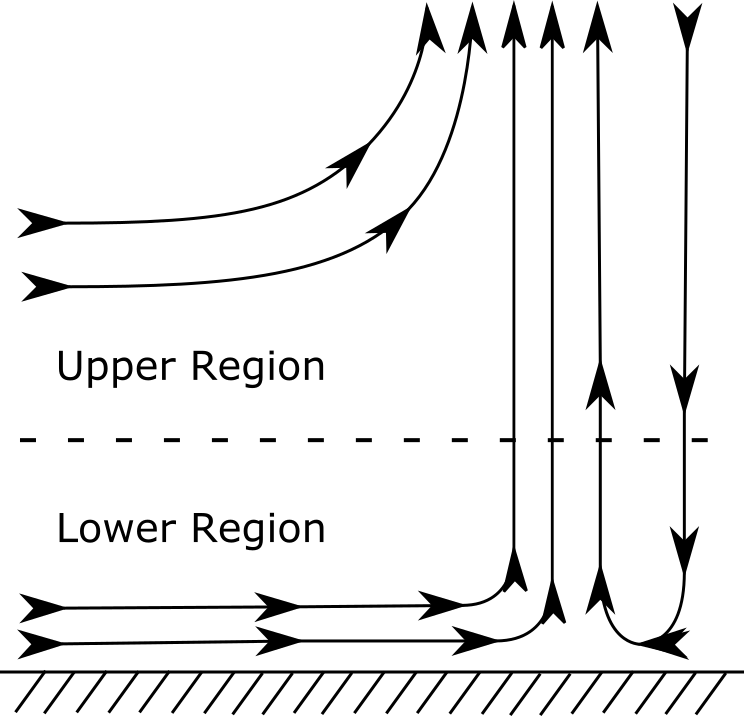
\includegraphics[width = 10 cm]{figs/ground}
     \caption{Cartoon of the structure of a dust devil. The lower region
     is the principle location of radial inflow, with the higher second
     layer flow becoming entrained by the upwardly circulating
     vortex. Notice also the downward flow in the center of the vortex.}
     \label{fig:cartoon}
    \end{center}
  \end{figure}


Renewed interest in naturally occurring dust devils has resulted from
the observation of them on Mars, first photographed by the NASA's Mars
Reconnaissance Orbiter\cite{}, and more recently by the Mars rover,
Opportunity. Their presence on Mars, with 1/100 of the atmospheric
density of the Earth, speaks to the universal character of the
phenomenon. Due to the greatly decreased atmospheric density, the
Martian dust devils are substantially larger, ranging several kilometers
across at their base and over ten km tall. 

interest in mixing and

There is lots of activity on dust devils and dust electrification now.  
The reason for this is that the ExoMars Lander will measure electric fields on Mars.

Numerical simulations of dust devils have been previously
reported.\todo{expand this greatly} However, they are typically large
eddy simulations (LES) that point towards the spontaneous occurance of
similar phenomena within existing 
climate and atmospheric
models\cite{QJ:QJ200513160722,doi:10.3137/ao.420105}. 


It is not clear what generates the azimuthal velocities. Two major
hypotheses as to the behavior exist. The first is that that ambient
vorticity in the atmosphere is drawn into the vortex from the far field,
and intensifies due to vortex stretching.\cite{} 

The other is that vortex tilting\cite{}

\section{Estimate of Energy Scaling}

Here we provide a rough estimate of the energy
available to a dust devil. There are two objectives of this
analysis. The first is to provide justification for the concept of
extracting energy from them, with the reasoning that should
sufficient energy be available, then attempting to extract it might be
worthwhile. The second objective is to provide a simple analysis that
can serve as a measure of the efficiency of the generation process,
e.g. ``What fraction of the available energy are we extracting?''.  

Steady state conditions requires that the dust devil not
extract more energy than is provided by the thermal resource, the Sun.   
The peak direct solar insolation in Arizona on a hot summer day is
greater than 1000 $W/m^2$. However, this estimate is problematic. 
It is in some sense an optimistic upper bound, as dust devils are only
converting a fraction of this solar resource into kinetic
energy. Renno and Ingersoll\cite{renno_inger} used an idealized heat
engine frame-work to study natural convection and to propose a theory
for convective available potential energy (CAPE), however, the
predictions from this underestimate the observed velocities in the real
objects. Furthermore, It is not clear how large of a region that dust
devils draw their energy from. Finally, dust devils are highly
intermittent creatures, typically existing only for a short time. It is
not certain that they are able to be accurately represented in a steady
state context. Lending some credence to this are the measurements of
\cite{} which found that surface heat fluxes could rise to . 

Sinclair's measurements of the velocity profiles inside a dust 
devil provides a more direct estimate. A velocity profile taken 
at approximately 9 meter height is shown in Figure \ref{fig:sinclair_profile}. 

  \begin{figure}[!htb]
    \begin{center}
     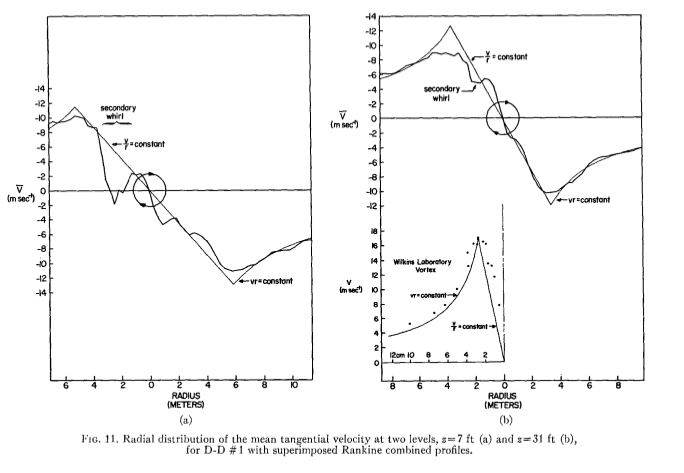
\includegraphics[width = 20 cm]{figs/sinclair_cut}
     \caption{Sinclair Profile}
     \label{fig:sinclair_profile}
    \end{center}
  \end{figure}

This is a dust devil with an inner core radius of approximately 
6 meters, and tangential and axial velocities of 11 and 10 m/s, respecively. 
This profile can be integrated to provide an estimate of the power though this plane, 
\begin{equation}
 P = -\frac{\rho }{2} \int V_z (V_{\theta}^2 + V_z^2 ) dA, 
\end{equation}
which results in an estimate of 24 kW. This is a substantial amount of
energy. 

%
% show what sinclair measured, then show how we think these energies
% break down into kinetic vs wind
%

As alluded to above, the energy composition of these flows is of
interest. For instance, Carroll and Ryan\cite{JGR:JGR14185} %1970
found that the kinetic energy contained within a dust devil exceeds that
which is attributable to buoyancy. Furthermore, Kaimal and Busigner
observed that dust devils possessed an order of magnitude greater
vertical flux in kinetic and than similarly sized convective
plumes~\cite{doi:10.1175/1520-0450(1970)009<0612:CSOACP>2.0.CO;2}. The
interplay between rotation, ambient winds and thermal potential energy
are critical to velocity intensities observed in these phenomena. 

As an example of this, consider only the energy flowing into the
entrainment region due to the ambient conditions, in particular, the
incoming wind and heat flowing through a cylindrical region. A
medium-sized (3m radius) dust devil with an incoming 
freestream velocity of 5 m/s. The surface temperature is 343 Kelvin,
with a specified inflow boundary layer bridging the ground temperature
to the ambient air conditions of 313 Kelvin.\todo{convert to same as
estimate above?}
% cite this?
\footnote{\normalsize These numbers were selected based on information
provided by the Georgia Tech field team from measurements performed in
Arizona during the summer of 2014.} 

There are two forms of energy to consider: kinetic and gravitational
potential. First, we examine the kinetic energy flux through the front
of the apparatus. 
%From the first law of thermodynamics we can express
The kinetic energy flux is a surface integral over the upstream face of
the device,  
\begin{equation*}
\text{KE} = \int \frac{\vec V^2}{2} \rho \vec V \cdot \hat n \, dA.
\end{equation*}
%
% could cite fluid dynamics book here
% pg. 239
%
Several simplifying assumptions are made. The freestream 
velocity is assumed to have no components in the span and height and
the variation in height of the streamwise
velocity is only due to the thin boundary layer near the
ground. The boundary layer profile is modeled using the common 7th
power function for a turbulent boundary layer,  
\begin{equation*}
  u(z) = U \text{ min }\left(\left(\frac{z}{\delta}\right)^7,1\right)
\end{equation*}
where U is the constant freestream velocity and $\delta$ the assumed
boundary layer thickness. 
The result for the kinetic energy is then, 
\begin{align*}
\text{KE} & = R \rho U^3 \left[ z_{\text{max}} - \frac{10}{11}\delta
\right].
\end{align*}
Where R is the radius of the vortex. Typical values of these quantities
are, $U = 5$ m/s, $\rho = 1.225$ Kg/$\text{m}^3$, $R = 3$ m,
$z_{\text{max}} = 2.5$ m and $\delta \approx 10$ cm. This provides an
estimate of 1144 Watts as the incoming kinetic energy flux. 

The gravitational potential energy flux is estimated by integrating the
boussinesq potential energy flux over the upstream flow. 
This is the maximum energy that could be extracted from the flow by an 
adiabatic redistribution of the density variation from the ambient 
density of the freestream flow, $\rho_\infty$. 
This potential energy ($E_p$) has the form of a surface integral over 
the front half of the vanes, 
\begin{align*}
  E_p & = \int u(z) (\rho(z)-\rho_\infty) g z dA. 
\end{align*}
As the density only varies with height, the integral is simplified to only vary in 
this direction
\begin{align*}
  E_p  & = g \int^{z_\text{max}}_0 u(z) (\rho(z)-\rho_\infty) \, z  \pi
 R \, dz.
\end{align*}
Using the bousinesq approximation, $(\rho(z)-\rho_\infty)  = \rho_0 \beta \Delta T$,
%\begin{align*}
%   (\rho(z)-\rho_\infty) & = - \rho_0 \beta \Delta T 
%   (\rho(z)-\rho_\infty) & = - \rho_0 \beta (T(z) - T_\infty),
%\end{align*}
the integral becomes, 
\begin{align*}
  E_p & = g  \pi R \beta \rho_0 \Delta T \int^{z_\text{max}}_0 u(z) \, z dz.
\end{align*}
This is solved to show
\begin{align*}
  E_p & = g  \pi R \beta \rho_0 U \Delta T \left[ \frac{z_\text{max}^2}{2} - \frac{7 \delta^2}{18} \right].
\end{align*}

%
% \todo{check units}
% 
% lets check the units here--
%
% m/s m^3 1/T kg/m^3 m/s T
%
% = Kg M^2 / s^3
%

%Once again assuming the 7th order power function for a turbulent boundary layer, 
% old text:::
%% \begin{align*}
%%   \text{Potential Energy Flux} & = \int_{-z_\text{max}}^0 u(z) \Delta \rho g z dz. \\
%%   & = \int_{-z_\text{max}}^0 u(z) \rho' g z^2 dz. 
%% \end{align*}
%% Where the substitution, $\Delta \rho = \rho' z$ was made. We again
%% assume the boundary layer follows the 7th order profile, and 
%% that $\rho' = -\beta \rho_0 \Delta T$, resulting in, 
%% %
%% % cite monin-yaglom page 59
%% %
%% \begin{equation}
%%  \text{Power } = U \beta \rho_0 \Delta T g \left[ \frac{z_\text{max}^3}{3} -
%% 					    \frac{7}{30} \delta^3
%% 					   \right]. 
%% \end{equation}

Characteristic values for a dust devil are $\rho_0 = 1.225$ Kg/$\text{m}^3$, 
$\Delta T= 30$ Kelvin, $\beta = 0.003194$ (This is 1/$T_{\text{ground}}$), 
$R = 3 $ m, $z_\text{max} = 2.5$ m, $\delta \approx 10$ cm, $g=9.81$ m/$s^2$, and a
freestream velocity of five meters per second results in an estimate of 34 Watts %33.82 Watts 
for the gravitational potential energy. 

The majority of the available energy is thus in the kinetic energy of
the wind, not the gravitational potential energy of the actual air. 
% todo: think about renno
%This is inconsistent with the results of
%Renno\cite{}\todo{missing cite here}, who demonstrated
%that the available thermal energy present was not sufficient to account
%for the velocities measured in dust devils. 
However, while the gravitational potential energy is a small fraction of
the energy available, that does not imply it is without significant
impact. 
%The extent to which the thermal energy acts as an assisting mechanism for 
%``lifting-up'' the flow is unclear, but 
Given the observed increase in dust devil formation during peak thermal
gradients, it is expected to play an important role. 

\section{Previous Concepts for Extracting Gravitational Potential
 Energy}

cite\todo{des it even make sense to write much here?}

cite\todo{cite mark thesis}

%
% https://en.wikipedia.org/wiki/Vortex_engine
%
% https://en.wikipedia.org/wiki/Solar_updraft_tower
%
% https://upload.wikimedia.org/wikipedia/commons/8/8b/Smoke-jack.jpg
%
% http://vortexengine.ca/AVE_FAQ.shtml
%
% http://ir.lib.uwo.ca/etd/89/
%
% http://www.popsci.com/technology/article/2012-12/paypal-cofounder-funds-tornado-harnessing-power-generator-produce-cheap-clean-energy
%
% Philosophies and fallacies in turbulence modeling --citation
%
% http://www.numerik.uni-hd.de/Oberwolfach-Seminar/CFD-Course.pdf
%

\section{Dust Devil Generation Concept}

The preceding discussion suggests that dust devils are carriers of
significant levels of ambient kinetic and gravitational potential energy
from the environment. This subsection provides a brief discussion of how
the physics of dust devils informs the generation of a synthetic
variety, that might be used as a means of extracting usable work.  

In contrast to the naturally occuring dust devils,
our synthetic solar driven vortex (SoV) design makes use of
control surfaces. These turning vanes also serve as an anchor for the
synthetic vortex, locking it into a small region. An abstract concept of
the turning vane geometry is shown in Figure \ref{fig:cartoon_vanes}.

  \begin{figure}[!htb]
    \begin{center}
     \includegraphics[width = 8 cm]{figs/ground_vanes}
     \caption{Image of a possible two tier turning vane 
       configuration for generating synthetic dust devils. This image depicts a 
       vertical slice through the proposed configuration, and does not show the reflection 
       of the two tier turning vanes, which would be expected to encircle the dust devil core.}
     \label{fig:cartoon_vanes}
    \end{center}
  \end{figure}

% Our observations of the naturally occuring dust devils informs some of
% our \textit{a priori} expectations for the design of the turning
% vanes. The bottom tier are designed to reside in the lower region, where
% the principle inflow will occur. We therefore expect a radial or nearly
% radial start to the vanes, which becomes increasingly tangential as the
% flow moves towards the center. The inner radius of the bottom tier will
% correspond to the outer radius of the generated vortex. 

% The top tier serves a different purpose. We expect a non-zero initial
% angle, as this tier is also designed to protect the rising vortex from
% being blow away by ambient winds. The vanes radius will be shorter, as
% the flow from this tier becomes entrained and the vortex grows in
% size. 

% For both the upper and lower tiers, our objective is to strike a balance
% between effectively turning the incoming flow to impart azimuthal
% velocity, while simultaneously not introducing such a high angle that
% the vanes act as a blocking surface which the incoming flow will move
% around. For instance, when the inlet angles are too severe, the vanes
% block the incoming flow, which results in an adverse pressure gradient
% existing near the outside edge of the 
% vanes. This serves to force fluid around and over the system, instead
% of inside the turning vanes. This reduces the velocity of flow inside
% the system, resulting in a weaker thermal vortex.  To reduce
% the flow blockage, we use gently curving vanes. A gentler angle permits
% more flow to enter the vane region, after which the curvature increases
% toward the center of the vanes. In this way, the angle smoothly varies
% between a nearly zero angle at the outside edge of the vanes to a
% maximum angle at a specified inner radius.

The characteristics of natural dust devils shown in Figure
\ref{fig:cartoon} suggest that the turning vanes be structured with two
tiers (see Figure \ref{fig:cartoon_vanes}). The lower tier would be
designed to manipulate the surface layer 
that lifts up into the core of the vortex, while the upper tier would
control entrainment into the vortex. In both tiers, the design of the
turning vanes must balance between the need to turn the flow from the
radial direction to the azimuthal direction to create vortical motion
and the requirement to not block flow into the vortex. Furthermore, in
the presence of a cross wind, the vanes need to prevent flow that
would pass right through the device, which would disrupt the vortex.
Finally, in field tests of design concepts for a solar vortex device
conducted by our colleagues at the Georgia Tech, it was found that cross
winds over the facility will also disrupt the vortical flow, and that
this could be controlled by introducing a conical wind-block on top of
the upper tier of vanes. One such field test configuration is shown in
Figure \ref{fig:field_test}. Within this broad conceptual design, there
remains a large design space to explore, including design parameters for
both tiers of vanes and the wind-block cone.

  \begin{figure}[!htb]
    \begin{center}
     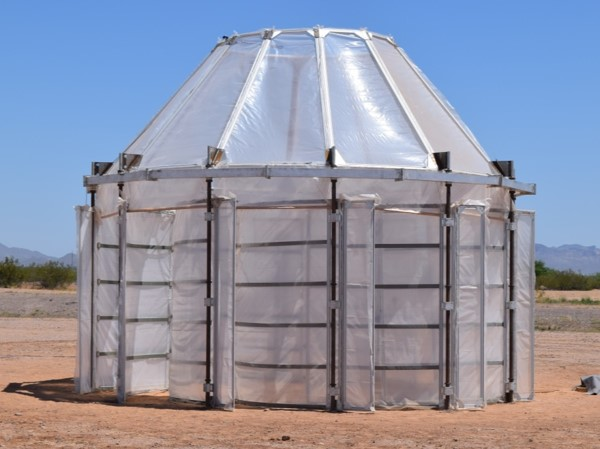
\includegraphics[width = 8 cm]{figs/sov_field}
     \caption{An image of the field configuration from the June, 2015
     tests in Arizona. The second (upper) tier of vanes and the cone are
     clearly visible. This apparatus has an outer diameter of
     approximately three meters.}
     \label{fig:field_test}
    \end{center}
  \end{figure}

To extract energy from the synthetic dust devil formed by the vane
system described briefly above, a turbine would be placed near the top
of the upper vanes. The turbine would extract energy from both the
vertical and azimuthal flow in the vortex, and so the design
considerations are different from those for a classical wind turbine.
Furthermore, there is presumably an analog to the Betz limit on how
much of the energy can be extracted, without disrupting the flow so
much that the vortex cannot be maintained. This will need to be
explored as part of the turbine design process.

In the research proposed here, the design and performance of a dust
devil energy harvesting system will be explored using computational
models. Computer models will enable a more extensive exploration of
the design space than would be possible experimentally. The design
concept described above will be analyzed to maximize the the
power that can be generated by the system and to develop scaling
describing how power depends on device size, wind speed and thermal
conditions. Further new design concepts that may be formulated will
also be evaluated. The subsequent section will provide the mathematical
representation used to model the system.  

%
%
%

% Our principle objective is to use a synthetic dust devil to produce 
% usable work. To extract the energy from the synthetic dust
% devil, a turbine is placed 
% at or near the top of the second tier of turning vanes. 
% The blades of the turbine will be driven by the dust devil's azimuthal
% and vertical velocities. While the Betz limit\cite{betz} gives a reasonable
% expectation of the efficiency with which energy can be expected to be
% extracted from the ambient dust devil velocity field, there are other
% non-trivial design considerations. In particular, the impact of the
% turbine on the dust devil's vortex, and any potential disruption of the
% flow on account of the turbine must be investigated. Optimizing the
% turbine to maximize the energy extraction while simultaneously
% minimizing it's impact on the character of the dust devil's solution
% will be an important issue.

% While the turning vanes and turbine  
% paradigm represents a reasonable starting point for design, the
% parameter space of possible system configurations is large. It is
% unclear how to engineer an effective SoV system. Important design
% consideration include: 
% \begin{itemize}
%   \item How should the turning vanes be configured?
%   \item How does the energy produced scale with system diameter?
%   \item Are additional surfaces, such as a cone, capable of increasing energy output?
% \end{itemize}

% Questions such as these provide the principle impetus of using
% computational fluid dynamics (CFD) to inform system design. The
% parameter space of conceivable system designs is far larger than can be
% probed experimentally, and even if such a campaign were to be embarked
% upon, it would be at significantly greater temporal and monetary
% cost. The subsequent chapter will provide the mathematical basis by which
% we model the system, so that we can then begin to discuss how we might
% optimize it computationally.  




\chapter{Mathematical Modeling}
%\section{Mathematical Modeling}
\label{sec:mathmodel}

% \begin{itemize}
% \item \st{unstable stratified boundary layers (raleigh number estimate)}
% \item \st{justify incompressible N-S}
% \item \st{justification of far-field eddy-viscosity model (M-O)}
% \item modeling eddy-viscosity in device 
% \item vane and turbine representation via penalty function // immersed boundary method
% \item cone representation
% \end{itemize}

%remember that \st{} is strikethrough
%
% should this all be math modeling?
%

The aim of this work is to simulate synthetic
dust devils in the field. This requires a model of the ambient
conditions for a representative case, such as Arizona, where
experimental data is available from tests that have been
performed. Furthermore, for this to be generally useful in the
prediction of flows in a variety of conditions, we need a model
applicable to any flow near the surface of the earth.  

This chapter details an analysis of surface fluid mechanics, and
develops a mathematical model for turbulence in a thermally stratified
medium. We seek to emulate the operation of the apparatus during the
day, when dust devils are observed to form readily. 
At these times, the atmospheric surface layer has the following
character. Incident radiation from the Sun does not significantly
interact with the air, which is nearly
transparent\cite{haltiner1957dynamical}. Instead, this radiation is
absorbed by the ground, which causes its temperature to rise. This
results in a temperature difference between the hot ground and the cooler
air. The sensible heat causes expansion and lowers the density
of the air. This reduced density air near the surface is then driven
upwards by buoyancy.    

For sufficiently large temperature differences, the hot surface layer is
unstable, and as the warm air is driven upwards the flow will transition
to turbulence. For the typical use case we consider, namely Arizona in
summer, the temperature difference can be in excess of 30 Kelvin. 
Rayleigh numbers associated with temperature differences of this
magnitude are between $10^{9} - 10^{11}$ and therefore meets the
criterion\cite{incropera1996fundamentals}  
for transition to a turbulent regime. The flow is that of an unstably
stratified fluid.  

This chapter begins by describing the governing equations of the system
of interest. It then proceeds to the development of a viscosity model
used to resolve the large scale features of the solution. Next, models
used to represent the vanes and turbine, are introduced.  Finally, the
models for the computational domain extent and the boundary conditions
are discussed. 

%Note that a complete numerical specification of all the model
%parameters introduced in this chapter are provided in a table in
%appendix \ref{app:model_param}.

\section{The Governing Equations of Fluid Motion}
\label{sub_sec:ns_en}

The equations describing fluid flow with natural convection are,
\begin{align}
  \frac{\partial {\bf u}}{\partial t} + {\bf u} \cdot \nabla {\bf u} =& \,
  -\frac{1}{\rho}\nabla P + \nu \nabla^2 {\bf u} - {\bf g} \frac{T'}{T_0}
 \label{eq:ns} \\
  \nabla \cdot {\bf u} =& \, 0 \label{eq:cont} \\
  \rho c_p \frac{\partial T}{\partial t} + {\bf u} \cdot \nabla T =& \, \nabla
 \cdot ( k \nabla T) \label{eq:ht}
\end{align} 
under the assumption that the temperature variation is small in
comparison to the mean temperature of the region. These are the
incompressible Navier-Stokes equations with the Boussinesq
approximation\cite{boussinesq2010théorie}, a representation of buoyancy
coupled with the heat equation. Note that in
Equations~\ref{eq:ns}-\ref{eq:ht}, and throughout this document,
boldface denotes a vector quantity, for example, ${\bf u} = \{u,v,w\}$.  
Further these equations ignore the action of the Coriolis force. 
Monin and Obukhov~\cite{monin1954basic} demonstrated that the Coriolis
force is negligible for the surface layer below fifty meters (a distance
well below our region of interest), and this argument is detailed in
Appendix~\ref{appendix:coriolis}.  

As discussed above, we anticipate that the flow will be sufficiently
high Reynolds number as to be
turbulent~\cite{Reynolds01011883}. Turbulence significantly alters the
character of the flow,  
and necessitates either resolving the resulting small scales or
providing a model that represents their impact. In this case, a
Reynolds Averaged Navier-Stokes (RANS) formulation is used, where the 
turbulent viscosity and thermal conductivities are permitted to vary in
space, and the flow is decomposed into constant laminar and varying
turbulent and vane components,\todo{not always rans}  

\begin{eqnarray*}
 \nu =& \nu_{l} + \nu_{T}(z) + \nu_{V}(r,z) \\
 K =& K_{l} + K_{T}(z) + K_{V}(r,z).
\end{eqnarray*}

This is an effective eddy viscosity model\cite{boussinesq1887}, and the
subsequent two sections will elaborate on the spatial dependence and
character of $\nu_T$, $K_T$, $\nu_C$ and $K_C$. The laminar, base
diffusivities are $\nu_l$ and $K_l$, which do not vary in space.  

\section{Viscosity Model}

We use the well-known similarity model of Monin and
Obukhov\cite{monin2007statistical,1990JFM...212..637K} as
a guide to the specification of an eddy viscosity model to describe the
vertical mixing in the atmosphere. This formulation is an extension of
the mixing-length model of Prandtl, where the concepts of gradient
diffusion and mixing length were generalized to thermally stratified
flow.    

%ADD DIMENSIONS TO MAKE SCALING MORE CLEAR\todo{add dimensions}
%
% justify prandtl assumption here
%

Monin and Obukhov argued that under statistically stationary, horizontally
homogeneous conditions, the dynamics of any mean turbulent quantity
($\bar f$) in a thermally stratified medium depend only on,  

\begin{equation}
\bar f = f(z,\frac{g}{T_0},\rho_0,\nu_l,K_l,u^*,q).
\end{equation}
Aside from near the surface, the laminar diffusivities $\nu_l$ 
and $K_l$ will be  
small compared to their turbulent counterparts, $\nu_T$ and $K_T$, and 
are therefore negligible. 
The remaining five parameters are: the distance from the ground, z; the
buoyancy coefficient, $\frac{g}{T_0}$; the density of the fluid,
$\rho_0$; a velocity scale, $u^*$ (in particular, the freestream
velocity); and the heat flux to the ground, $q$. %\todo{is this right?}
% Likewise, if we define $z-z_0$ as an ``effective roughness
% height'' or displacement distance, we can reasonably neglect $z_0$ from these
% considerations. While the roughness height can be large (for instance in
% a cornfield, where the roughness height could reasonably be several
% meters), for the present study the expectation is that this roughness
% height will be on the order of centimeters\cite{oke1987boundary}, and
% therefore negligible.  
%
% add refence to dynamical and physical meteorology 
% 
These primary quantities have the following dimensions,

\begin{eqnarray}
 \textbf{Height:}& z\enskip \dot = \enskip [m]  \\
 \textbf{Buoyancy:}& \qquad \frac{g}{T_0}\enskip \dot = \enskip [kg] [m] [s]^{-2}
  [K]^{-1} \\ 
 \textbf{Density:}&  \enskip \rho \enskip \dot = \enskip [kg] [m]^{-3}  \\
 \textbf{Velocity:}& \enskip u^* \enskip \dot = \enskip [m] [s]^{-1} \\
 \textbf{Heat Flux:}& \enskip q \enskip \dot = \enskip [kg] [s]^{-3} 
 %\textbf{Height:}& z \rightarrow \text{Units}: Meters \rightarrow [m]  \\
 %\textbf{Buoyancy:}& \frac{g}{T_0} \rightarrow Units: Meters \rightarrow
 % [m]  \\ 
 %\textbf{Density:}& \rho \rightarrow Units:  \rightarrow
 % [m]  \\ 
 %b & b
\end{eqnarray}

Our unknown mean turbulent quantity ($\bar f$) depends on four
dimensions: length, time, temperature and mass. Dimensional analysis
implies that this should then only be a function of a single dimensionless
group\cite{munson2012fundamentals}. This is chosen to be,
\begin{equation}
 \xi = -\frac{\kappa \frac{g}{T_0} \frac{q}{c_p \rho_0} z}{ {u^*}^3}.
\end{equation}
where $\kappa$ is the (dimensionless) Von-Karman constant. 
The physical meaning of this quantity bears some discussion.  
The numerator, $\kappa \frac{g}{T_0} \frac{q}{c_p \rho_0} $, is
proportional to the buoyant production of kinetic energy.  The
denominator, $\frac{{u^*}^3}{z}$, is a shear production rate. 

The non-dimensional group $\xi$ is typically cast into the following 
form, 
\begin{equation}
 \xi = \frac{z}{L_{M-O}}
\end{equation}
where $L_{M-O}$ is the famous, ``Monin-Obukhov'' length,
\begin{equation}
 L_{M-O} = -\frac{{u^*}^3}{\kappa \frac{g}{T_0} \frac{q}{c_p \rho_0}}. 
  \label{eqn_mo_length}
\end{equation}

This length can be interpreted as the vertical location
where the production of buoyantly generated kinetic energy is
approximately equal to the energy generated by wind shear. When the
magnitude of $L_{M-O}$ is large, the flow is dominated by shear effects,
and the impact of buoyancy is small. Conversely, a small magnitude of
$L_{M-O}$ implies that buoyant effects largely dominate the kinetic
energy production. Notice also that the sign convention in Equation
\ref{eqn_mo_length} is such that for the systems we consider ($q > 0$, heat
flux from the surface to the air), $L_{M-O}$ will always be
negative. This is as expected, as the convection from the high
temperature surface to cooler air is unstable. 

%The mean quantity $\bar f$ has a
%functional representation to the effect,
In this case, appropriately normalized mean turbulent quantities should
be functions of only the non-dimensional group 
\begin{equation}
 \frac{\bar f}{f_{MO}} = \phi(\frac{z}{L_{M-O}})
\end{equation}
with $f_{MO}$ a normalizing constant with units of $\bar f$, and $\phi$
is a function only of $\xi$. Monin-Obuhkov similarity theory has been
shown to apply to a wide variety of
quantities\cite{wyngaard2010turbulence}, but we consider the velocity
and temperature fields here.  
Furthermore, we are interested in the case where
$\xi<0$, which corresponds to heat flux from the ground into the
air. For instance, the mean velocity field would have scaling,
$\frac{u^*}{\kappa}$ and the temperature fields would be scaled as $T^*
= \frac{1}{\kappa u^*} \frac{q}{c_p \rho_0}$. In this way, the mean
velocity and temperature fields would have the form,  
\begin{eqnarray}
\bar u(z) = \frac{u^*}{\kappa} \phi_u(\frac{z}{L_{M-O}}) \\
\bar T(z) = T^* \phi_T(\frac{z}{L_{M-O}}).
\end{eqnarray}
As a result, the mean vertical gradients of the velocity and temperature are
necessarily, 
\begin{eqnarray}
\frac{\partial \bar u(z)}{\partial z} = \frac{u^*}{\kappa L_{M-O}}
 \varphi_u(\frac{z}{L_{M-O}}) \label{eq:uz} \\ 
\frac{\partial \bar T(z)}{\partial z} = \frac{T^*}{L_{M-O}}
 \varphi_T(\frac{z}{L_{M-O}}) \label{eq:tz}.
\end{eqnarray}
Notice that $\phi$ and $\varphi$ are different (unknown) universal functions. Eddy
viscosity is defined as, $u'v' = \nu_T \frac{\partial
u}{\partial z}$\cite{durbin2001statistical}, in which case, using
equation \ref{eq:uz}, it must scale as
\begin{equation}
 \nu_T = \frac{{u^*}^2}{\frac{\partial \bar u}{\partial z}} = \frac{u^*
  \kappa L_{M-O}}{\varphi_u(\xi)}.
\end{equation}
While eddy thermal diffusivity (defined as, $q = c_p \rho_0 K_T
\frac{\partial T}{\partial z}$) is 
\begin{equation}
 K_T = \frac{q/c_p \rho_0}{\frac{\partial \bar T}{\partial z}} = \frac{u^*
  \kappa L_{M-O}}{\varphi_T(\xi)}.
\label{eqn:eddy_kt}
\end{equation}
Note the difference between $\varphi_u$ and
$\varphi_T$, which for turbulent Prandtl numbers near unity (e.g. $Pr_T
\approx 1$) the functions will be identical. The asymptotic behavior of
the $\varphi_T$ and $\varphi_u$ at large and small values of $\xi$
provides guidance to the more general character of the functions. 
Our interest lies in the case where $L_{M-O} \leq 0$, which corresponds
to heat flux from the ground into the air.  
%

\subsection*{Case One: $\xi \to 0$}
The first case, $\xi \to 0$, is equivalent to the scenario where
$\frac{z}{L_{M-O}} \to 0$, or $L_{M-O}>>z$. This occurs as the heat flux
at the wall approaches zero ($q \to 0$) , which is simply ``free
convection''. This would correspond to a purely wind driven flow with no
thermal gradient. In this limit, the solution is expected to regain the
thermally-independent result, the pre-eminent ``log-law''. Start by
considering Equation~\ref{eq:uz} rearranged into a slightly different form, 
\begin{equation}
 \frac{\partial \bar u(z)}{\partial z} = \frac{u^*}{\kappa L_{M-O}} \varphi_u(\frac{z}{L_{M-O}}).
\end{equation}
After substituting $L_{M-O}=\frac{z}{\xi}$, 
\begin{equation}
 \frac{\partial \bar u(z)}{\partial z} = \frac{u^*}{\kappa z} \xi \varphi_u(\xi).
\end{equation}
This is clearer if the substitution, $\Phi(\xi) = \xi \, \varphi(\xi)$, is made,
\begin{equation}
 \frac{\partial \bar u(z)}{\partial z} = \frac{u^*}{\kappa z} \Phi(\xi).
\end{equation}
One can now more easily see that this function results in a logarithmic
profile when $\Phi(\xi) = 1$, which in turn implies that for neutral
stratification $(\xi = 0)$, 
\begin{equation}
 \Phi(0) = \lim_{\xi \to 0} \, \xi \, \varphi(\xi)= 1. 
\end{equation}
We expect this to be approximately true for all small values of
$\xi$, e.g. 
\begin{equation}
 \Phi(\xi) \approx \text{ln } \rvert \frac{z}{L_{M-O}} \rvert + C 
\end{equation}
 when $ |\frac{z}{L_{M-O}}| << 1$. Identical arguments can be made for the
 asymptotic behaviour of the temperature function.

\subsection*{Case Two: $\xi \to -\infty$}

The case where $\xi \to -\infty $ implies $\frac{z}{L_{M-O}} \to
-\infty $ and $z>>L_{M-O}$. This is most readily interpreted as the instance
where $u^* \to 0$, e.g. the buoyancy-dominated case with no wind
(free-convection). This condition is typically referred to as,
``Thermal-only'' in this text. 
For this case, the function $\varphi_T$ must have no
dependence on $u^*$, and will approach a constant. Scaling
analysis implies that the overall function will not depend on $u^*$ only
when the function $\varphi$ scales to the $-\frac{4}{3}$ power. The
function must then be

\begin{equation}
 K_T = \frac{1}{C_T} \left( \frac{q}{c_p \rho_0} \frac{g}{T_0}
		     \right)^\frac{1}{3} z^{\frac{4}{3}}  \text{ 
for } z \gg L_{M-O}. 
\end{equation}

So long as the turbulent Prandtl number remains constant in space, a
realistic assumption~\cite{chuang1969turbulent}, then 
identical arguments regarding the asymptotic behaviour at large $\xi$
provide the analogous result for the eddy viscosity's variation with
respect to distance from the ground,   
\begin{equation}
 \nu_T = \frac{1}{C_{\nu_T}} \left( \frac{q}{c_p \rho_0} \frac{g}{T_0}
			     \right)^\frac{1}{3} z^{\frac{4}{3}}  \text{ 
for } z \gg L_{M-O}. 
\end{equation}


\subsection*{Approximations of the Universal Function}

We have now derived two criterion that our desired function of $\xi$ 
must capture. Namely, that for small values of negative $\xi$, the
function should be nearly identical to the logarithmic profiles
associated with neutral stratification. Secondly, at large negative
values of $\xi$, the function should approach a constant value. Finally,
we desire that the function smoothly vary between these conditions. 

Again following the lead from Monin-Obukhov, most functions are
formulated in terms of $\Phi(\xi)$, not $\varphi(\xi)$. Note that as
$\varphi(\xi) \thicksim \xi^{-\frac{4}{3}}$, and recalling that
$\Phi(\xi) = \xi \, \varphi(\xi)$, we expect 
$\Phi(\xi) \thicksim \xi^{-\frac{1}{3}}$.

There are several different functions, which are essentially different
calibrations of the same underlying function for different regimes with 
varying relative merits. %\cite{?}.\todo{missing cites} 
However, the functions are generally in close agreement under neutral
and unstable conditions, with the disagreement primarily occuring for
$z/L>0$. As we expect to only simulate conditions of unstable or
neutrally stratified flow, our choice of interpolation function does not
have a significant impact on the predicted value.  

\begin{figure}[!htb]
 \centering
  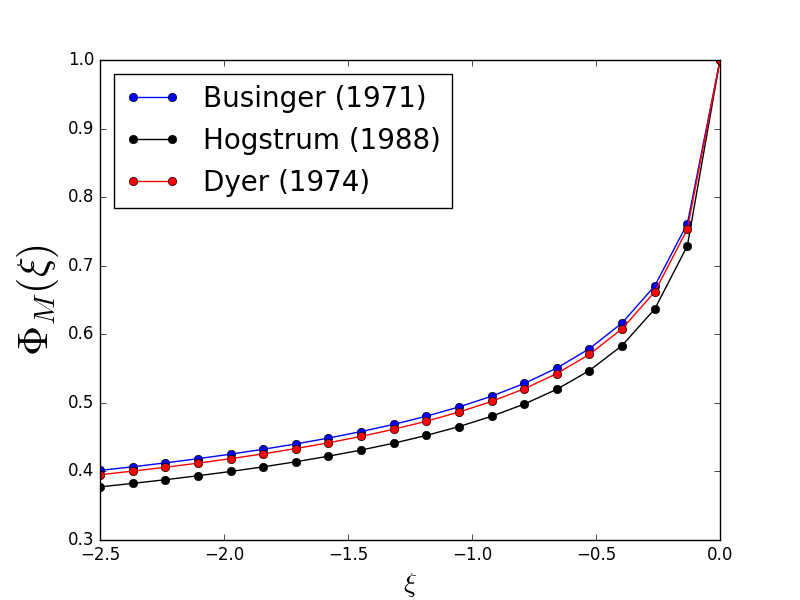
\includegraphics[width=.7\linewidth]{figs/mo-compare}\\
 \caption{Comparison between three common interpolation functions for
 the Monin-Obukhov universal function of momentum. The plots closely
 coincide, as the functions are generally in close agreement under
 neutral and unstable conditions, with the disagreement primarily
 occuring for $z/L>0$, which is unimportant for this work.} 
 \label{fig:interp-mo}
\end{figure}

Figure~\ref{fig:interp-mo} shows three common interpolation  
functions, the Businger~\cite{businger1971flux},
H{\"o}gstr{\"o}m~\cite{hogstrom1988non} and Dyer~\cite{dyer1974review}
functions. All have similar qualitative form,   
and yield nearly identical predictions. As a result, we use functions
that are simple to compute. The original functions 
proposed by Monin and Obukhov were avoided, they had a discontinuity in
the derivative, and are more inaccurate than modern functions due due to
the fact that they were calibrated on less accurate experimental
data. The H{\"o}gstr{\"o}m functions for momentum and temperature are, 
\begin{eqnarray}
  \Phi_M(\xi) =& (1-19.3 \, \xi)^{-1/4}, \\
  \Phi_T(\xi) =& 0.95 \, (1-11.6 \,\xi)^{-1/2}.
\end{eqnarray}
These functions have been found to be broadly applicable, accurate and 
are easily instantiated in software. For this reason the
H{\"o}gstr{\"o}m functions are used in this work. 

\subsection{Shortcomings of Monin-Obukhov Theory}

There are several well-known conditions for which the Monin
Obukhov similarity theory breaks down. These include:
 
\begin{itemize}
 \item Surfaces with large spatial variations in roughness
 \item Outside of the surface layer (several hundred meters) where the 
       coriolis effect is no longer negligible
%\item the theory's predictions are well known to be sensitive to choice
%      of universal function for $L>0$.
\end{itemize}

But neither of these are relevant here. 
In ``ideal'' situations, the theory has been found to be
accurate to better than 10\%\cite{QJ:QJ49709741204,kaimal}. 
For our case, with minimal surface roughness and our interest
constrained to the near surface layer, these functions are applicable
and reasonably accurate\cite{Foken2006}, and are easily implemented in
software.  

\section{Eddy Viscosity in the Device}

%However, this is also a more
%difficult regime to model.\todo{poor justification} 
The validation process identified a refinement to the virtual vane
formulation that results in a better representation of the vane
effects in a broader range of flows. The model uses an
enhanced turbulent diffusivity in the vortical plume region to account
for the effects of vortex shedding from the trailing edge of the vanes,
which is not represented in the virtual vane representation (discussed in
\ref{subsec:vane}). 

% To successfully accomplish this, source terms
% for production of diffusivity were formulated to properly
% account for the generation of turbulence in the region of the
% vanes. This diffusivity would then convect and diffuse through space. 
% To avoid modeling a temporal and three-dimensionally spatially
% varying field of diffusivities, we have instead calibrated the field
% based on data provided by our partners at Georgia Tech. 

%This calibration
%is detailed in Section~\ref{sec:validation}. 
The eddy-viscosity in the region of the vanes and interior is set based
on scaling relations for a turbulent self-similar circular jet, as
described in Pope\cite{pope2000turbulent},
 
\begin{equation}
  \nu_C = U_0 y_{1/2} \bar \nu_C.
  %\nu_C(r) = U_0(r) y_{1/2}(r) \bar \nu_C
\end{equation}

In this equation, $U_0$ is the peak velocity, and $y_{1/2}$ the jet
half-width (taken to be the dust devil half-width).  
% In words, we are scaling the
% calibrated viscosity by the velocity and length scale of the
% apparatus. $\bar \nu_C $ is input, measured from the experimental
% laboratory.  The diffusivity here is essentially a top hat filter, which
% radial values interior to the vanes the nominal calibrated value, and
% those outside the vanes zero, e.g. $\nu_C(r>r_{\text{vane}})=0$. 
The dimensionless constant $\bar \nu_C $ is calibrated based on
experimental data, and is set to zero outside the device. 
The thermal diffusivity inside the device, $K_C$, is then fixed with the 
assumption that the Prandtl number is unity.  

%The thermal and momentum diffusivities are expected to be even larger in the
%device where the flow across the vanes produces shear and generates
%turbulence. Our model for the diffusivities inside the vanes should
%therefore be higher than the ambient regions outside the vanes. 


\section{Vane Representation}
\label{subsec:vane}
To rapidly prototype general system configurations, the
computations must be able to explore a large space of possible
geometries and settings. This presents a significant meshing and 
computational challenge if the detailed flow around the vanes is to be
computed. In the region near the vanes, where a no-slip boundary
condition is imposed, the flow will necessarily form a thin momentum
boundary layer. Resolving this boundary layer requires high resolutions
immediately adjacent to the walls. Changing the vane location requires
that a new mesh be generated. This is a significant
challenge, as the development of a new mesh often requires significant
human effort and time. Furthermore, the process is error-prone, 
and would require that each simulation using a new mesh undergo 
detailed solution verification. 


% Your text on the virtual vanes does not provide enough information to
% know exactly what we did. It is needlessly vague, and does not
% adequately connect to the real vane geometry. I propose the following
% more direct and more precise text. Further, the penalty nomenclature
% is inappropriate.

Instead, we have developed a modeling formulation that does not require
explicitly meshing the turning vanes, or any surface. These so-called
``virtual vanes'' are implemented as a body force that 
is applied in the annular region that contains the vanes. 

   \begin{figure}[!htb]
    \centering
    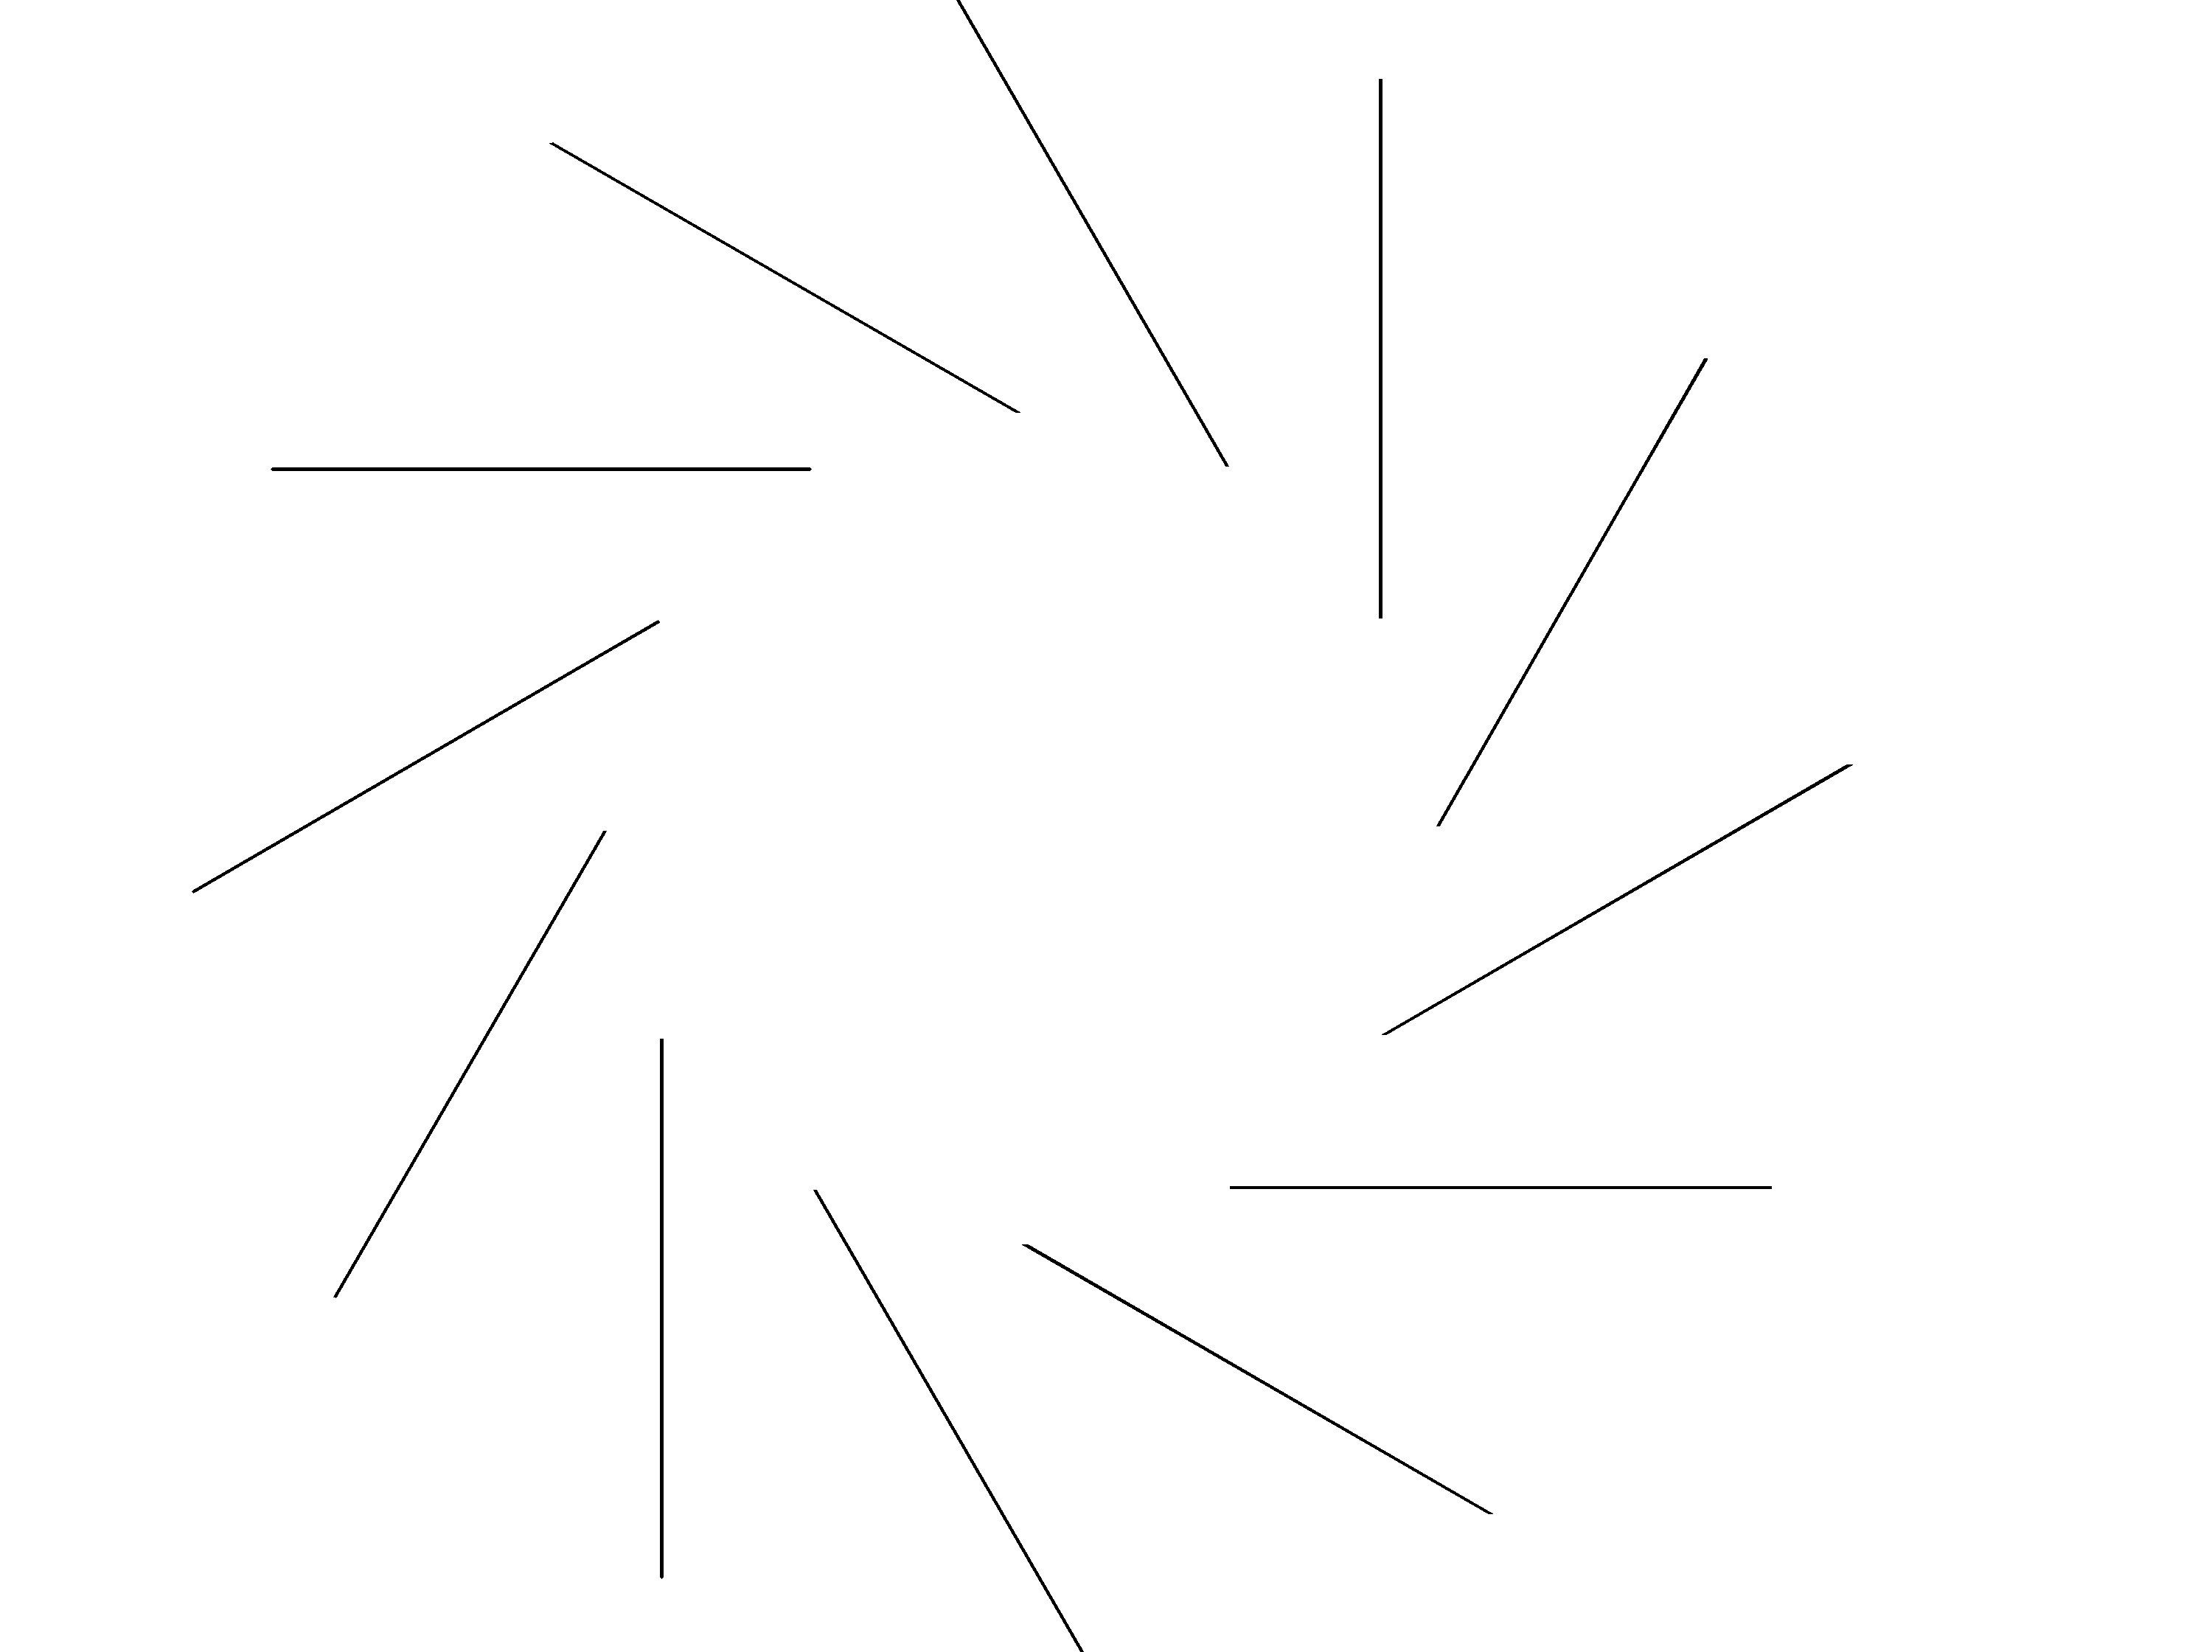
\includegraphics[width =0.47\textwidth]{figs/gridded_region}
    \hfill
    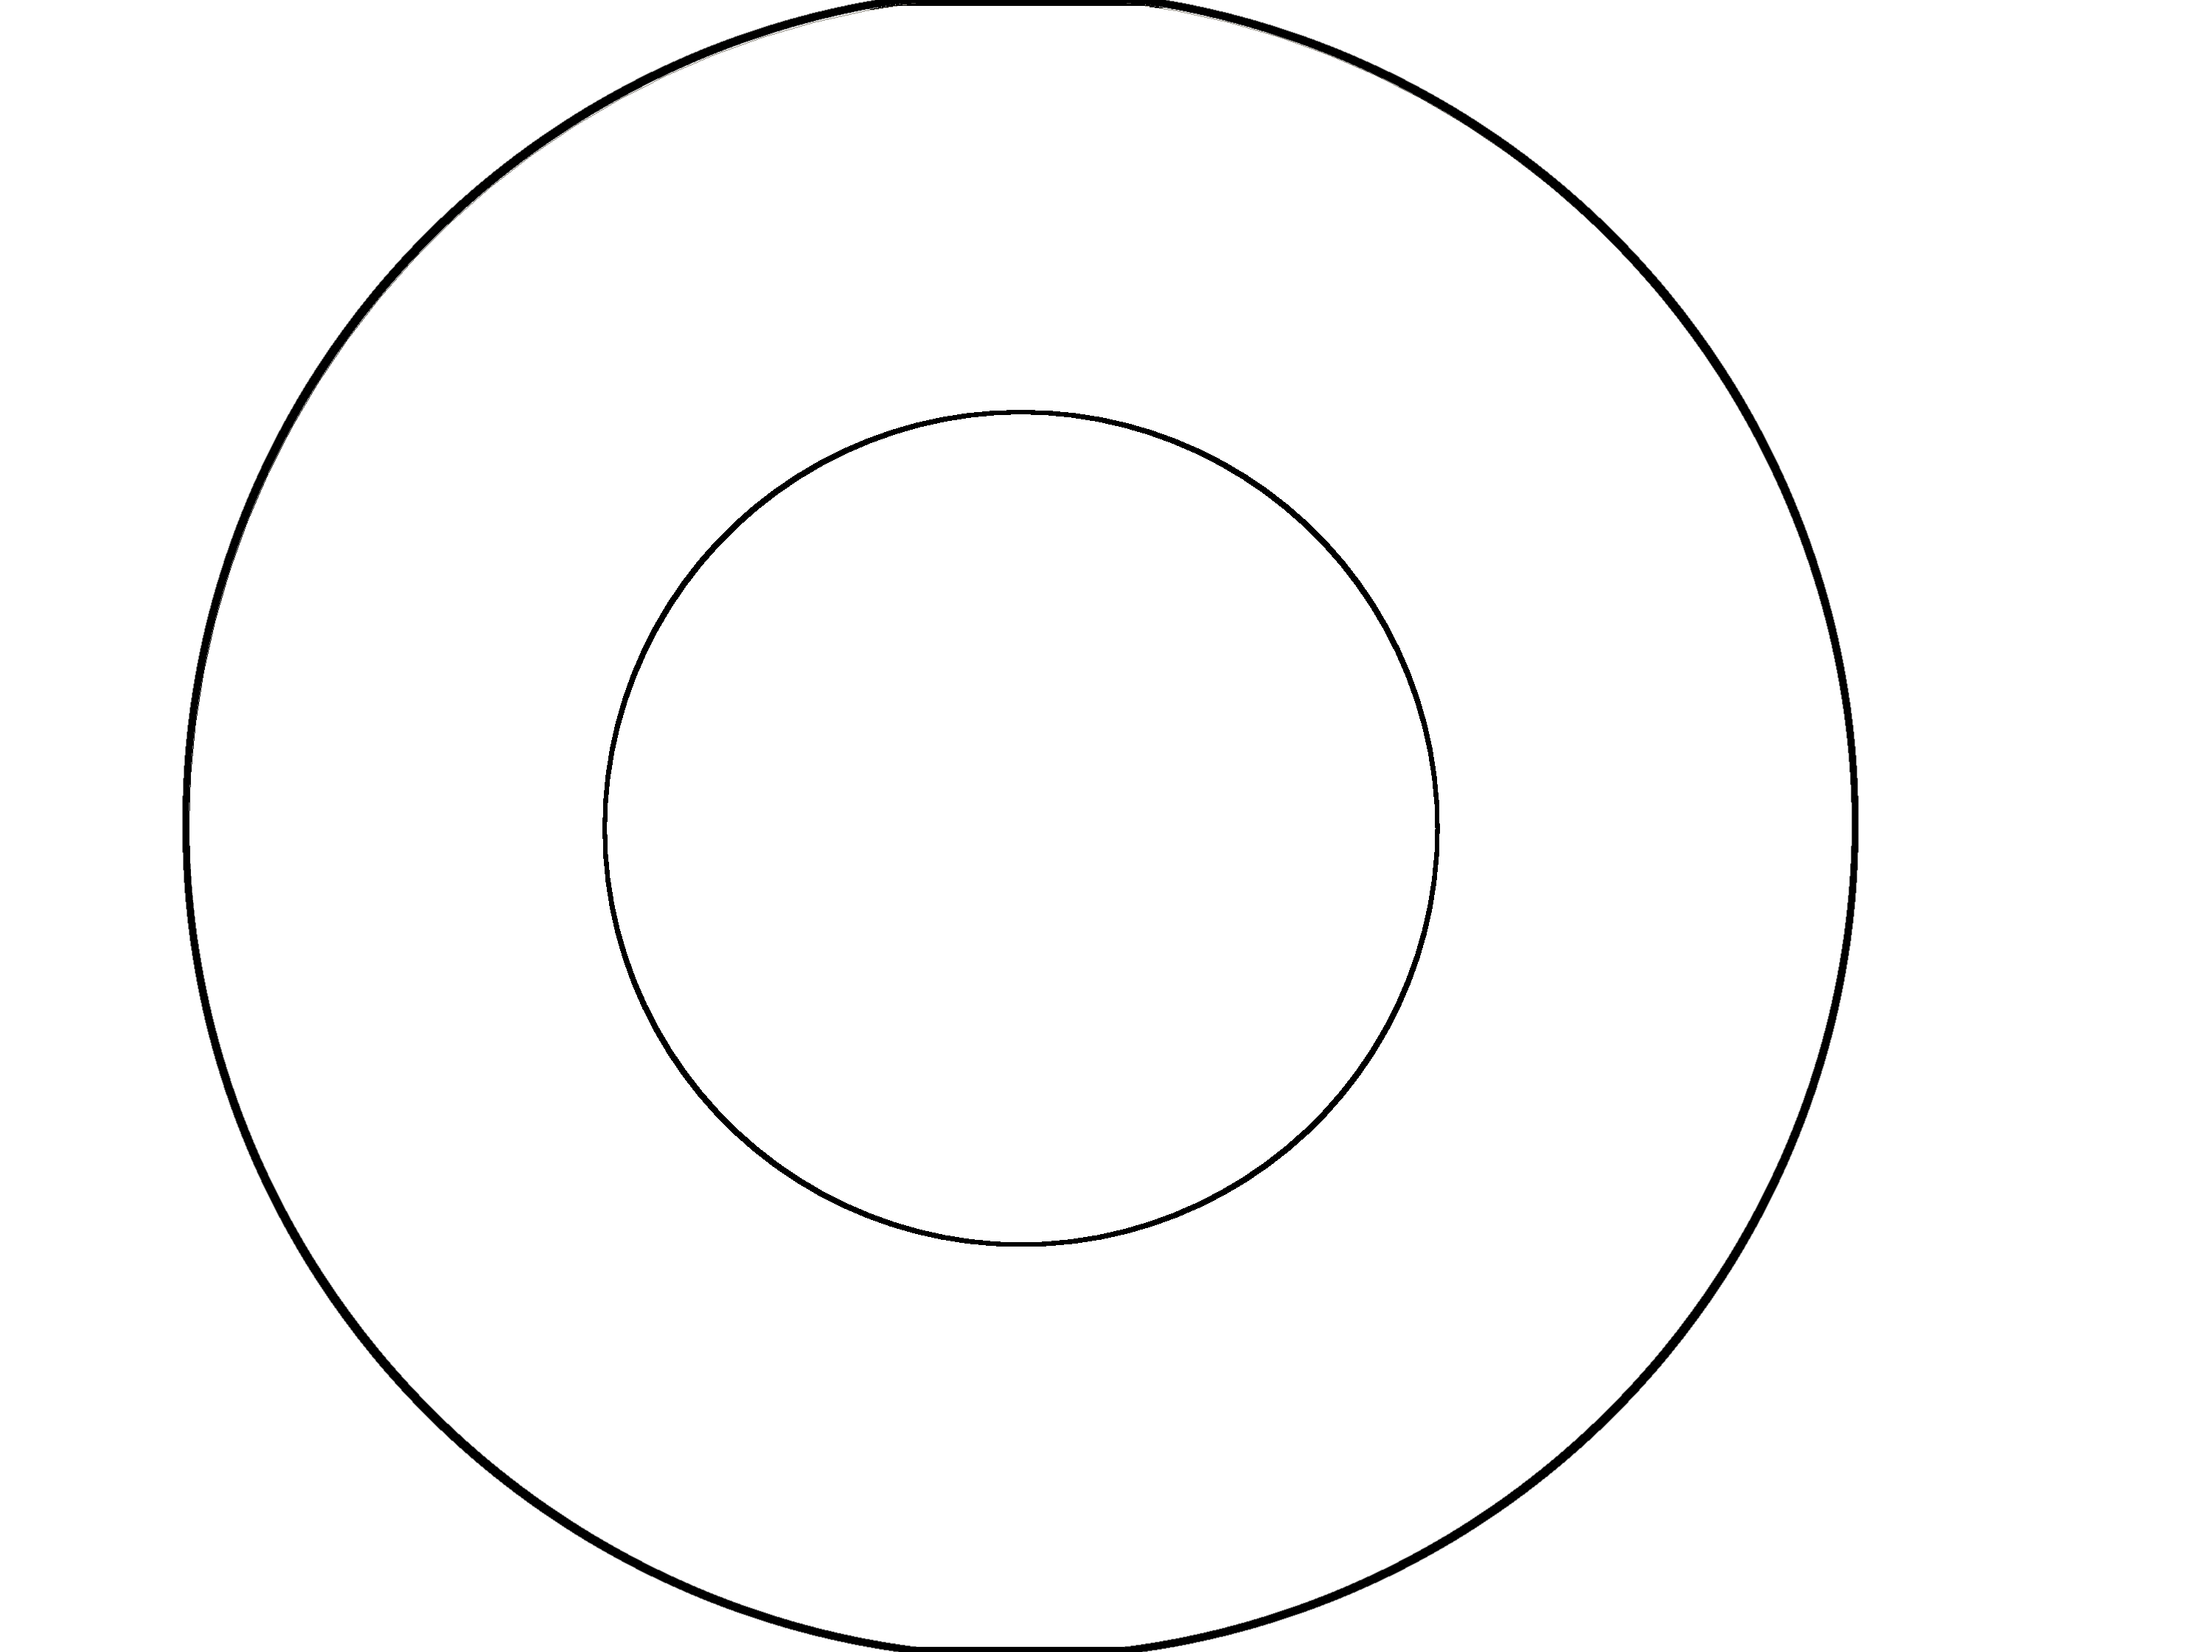
\includegraphics[width =0.35\textwidth]{figs/forcing_region}
     \caption{An example of explicitly represented turning vanes (left)
    versus an annular forcing region (right).}
     \label{fig:penalty_model}
   \end{figure}

Vane geometry is specified by the angle $\phi$ a vane makes with a
radial line as a function of the radial coordinate, $r$, and the polar
angle, $\theta$. A unit normal to the vane surface ${\bf n_v}$ is defined
as 
%
\begin{equation}
 {\bf n_v}({\bf x}) = \sin \left(\phi(r,\theta) \right) \hat{{\bf r}}+ \cos
  \left(\phi(r,\theta) \right) \hat{{\bf \theta}} 
\end{equation}
%
where $\hat{{\bf r}}$ and $\hat{{\bf \theta}}$ are unit
vectors in the radial and azimuthal directions, respectively.
With this vane-normal vector field specified, a body force ${\bf f_v}$
is defined that will drive the velocity in the ${\bf n}$ direction
toward zero, effectively turning the flow to be parallel to the
vanes. The body force is defined by,
\begin{equation}
 {\bf f}_v= -\frac{1}{\ell_v}|{\bf u}|({\bf u}\cdot{\bf n_v}){\bf n_v}
 \label{eqn:body_force}
\end{equation}
with ${\bf u}$ the velocity and $\ell_v$ is a specified length
scale. $\ell_v$ represents the distance over which the
flow evolves under the influence of the body force before the
velocity in the normal direction is reduced by a factor of $1/{\bf 
e}$.
That is, this is the length over which the normal component of the
velocity decays exponentially. 
%It is the distance analog to the more
%familiar time constant of exponential decay. 

Therefore, $\ell_v$ is a modeling constant and must be specified. Our
expectation is that it will be the same order as the separation distance
between neighboring vanes in the physical vane configuration, since
entry  lengths in internal flows scale with the width of the
channel. This study\todo{what study, describe what i did} is depicted in
Figure~\ref{fig:annealing}, where the average misfit between the turning
vane angle in an explicitly represented vane configuration and the flow is plotted.   

The trend is clear that as the flow moves through the turning vanes
towards the center of the apparatus it is brought into alignment with
the turning vane direction. 
Notice that the misfit actually grows near the minimum, likely due to
unmodeled transient effects such as vortex shedding off the vane
trailing edges. 

   \begin{figure}[!htb]
    \centering
    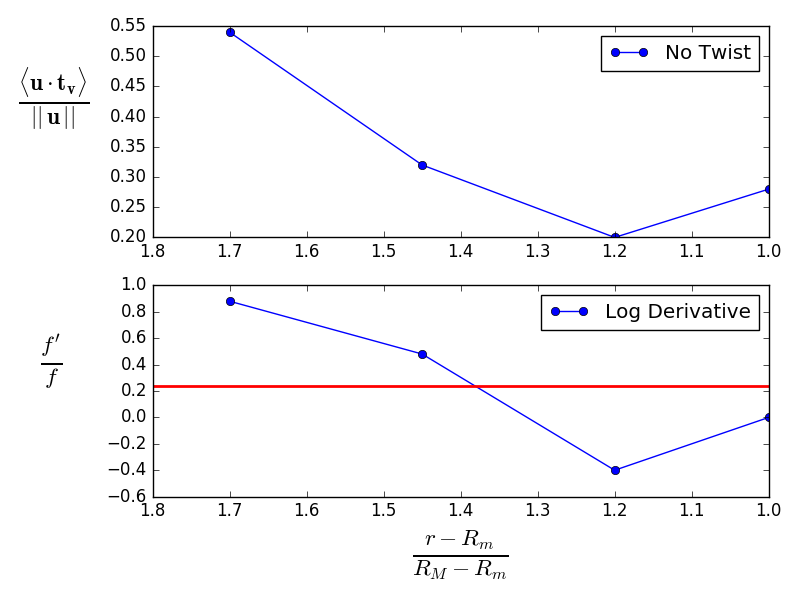
\includegraphics[width =0.8\textwidth]{figs/annealing}
     \caption{The average misfit between the gridded vanes and the
    flow. The averaging is accomplished through azimuthal
    averaging. This was taken at half the height of the turning vanes,
    although the results do not differ at greater or lower height. 
    The subfigure shows the logarithmic derivative, as well as the
    average of the logarithmic derivative in red. 
$R_{M}$ is the furthest radial extent of the gridded vanes,
    and $R_{m}$ the smallest radial extent. The subfigure shows the
    logarithmic derivative of this quantity.}
     \label{fig:annealing}
   \end{figure}


Now, $\ell_v$ can be calibrated to explicitly match the results of the
gridded vanes by assuming that the vane mismatch obeys a radial
exponential decay of the form $f(r) = A e^{-\ell_v r}$, and taking the
logarithmic derivative of this quantity, 
\begin{eqnarray}
 \frac{f'}{f} = \frac{A e^{-\ell_v r} * -\ell_v}{A e^{-\ell_v r}} =
  -\ell_v. 
\end{eqnarray}

This is shown in subfigure of Figure~\ref{fig:annealing}, where we would
expect a flat line if the misfit between vanes was perfectly described
by an exponential decay. While the curve does not perfectly coincide
with this, the curve does not have severe convexity and the average is
sufficient for this work. Based on this, the lengthscale $\ell_v$ was
set to three\todo{what? it has dimension}. 

%\todo{show
%calibration of this} 

This virtual vane formulation is similar to the ``actuator disk'' model
commonly used to represent the rotor of a wind turbine and
described in the subsequent section. 

\section{Turbine Representation}
\label{sec:actuator_disk}
%
% https://en.wikipedia.org/wiki/Blade_solidity
%

The turbine is modeled similarly to the virtual vanes. As with the
vanes, it is desirable to avoid explicitly representing the turbine
blade control surfaces. Instead, the turbine is modeled using the
actuator disc simplification. 
This model (also often referred to as a ``Blade Element Momentum''
theory) is commonly used in wind
turbine design\cite{shevell1983fundamentals,betz,leclerc}. The essence
of this model is to approximate the individual spinning turbine blades
as a ``disk'' in which the effects of the turbine are represented by
body forces on the fluid, as shown in Figure~\ref{fig:actuator_disk}.
This method assumes an axisymmetric representation of the turbine
geometry, and in doing so completely neglects unsteady effects due to
the rotation of turbine blades in a plane. 

As the flow moves through the actuator disk, it experiences a force
normal to the represented turbine blade surface. This force will
generally be in opposition to the flow direction, and will therefore
impart a loss of momentum on the fluid. 
Associated with the loss of axial and azimuthal momentum is a loss of
energy which can be collected by an electrical generator attached
to the rotor shaft if the rotor experiences a torque
in the direction of rotation. 

All the turbine cases shown in this study make the further
simplification that the rotation speed of the disk is constant. 
In this way it is assumed that the turbine exerts a torque equal and
opposite to that of the airflow which keeps the rotational speed
constant. The work done by the aerodynamic torque on the
turbine is assumed to feed into a generator, where it is converted into
electrical energy. 


   \begin{figure}[!htb]
    \centering
    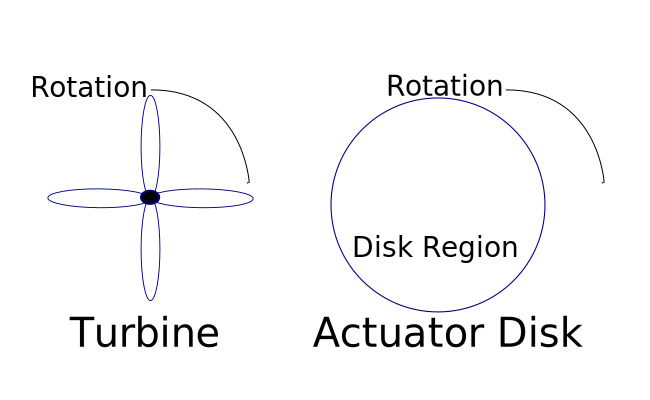
\includegraphics[width =0.95\textwidth]{figs/actuator_disk}
     \caption{The actuator disk model represents a turbine blade
    geometry (shown on the left) as a spinning ``disk'' region (shown
    on the right).}
     \label{fig:actuator_disk}
   \end{figure}

We now detail the mathematical machinery necessary to specify the
direction and magnitude of force between the turbine and flow. The
normal in the blade's velocity direction is, 
\begin{equation*}
n_B = \frac{{\bf u_B}}{||{\bf u_B}||}. 
\end{equation*}
Where ${\bf u_B}$ is the blade velocity vector and is specified. The
normal in the fan vertical direction is typically ${\bf n_f} =
\left(0,0,1\right)$, e.g. pointing ``up''. Then the normal in the radial
direction must be,  
\begin{equation*}
{\bf n_r} = {\bf n_B} \times {\bf n_f}
\end{equation*}

% The fan-wing-plane bit means that we're only looking at the projection
% of velocity into the plane that's defined by the base velocity and
% vertical direction. 

% (01:03:44 PM) Roy Stogner: The "local relative velocity" means that
% we're taking the velocity not in the reference frame of the domain, but
% in the reference frame of the wing.  So if the base velocity is U_B and
% the air velocity is U, then the local relative velocity is U - U_B. 
% (01:04:25 PM) Roy Stogner: Note that we simplify that equation a tiny
% bit by using the fact that U_B and N_R are perpendicular. 

and the fan-wing-plane component (e.g. the plane perpendicular to the 
radius) of local relative velocity is
\begin{equation}
{\bf u_p} = {\bf u} - ({\bf u}\cdot {\bf n_r})\cdot {\bf n_r} - {\bf u_B}. 
\end{equation}
This is the projection of velocity into the plane defined by the base
velocity and vertical direction. Now the ``forward velocity'' in the
reference frame of the turbine is,  
\begin{equation}
{\bf u_{\text{fwd}}}= -{\bf u_p} \cdot {\bf n_B}
\end{equation}
and the ``upward'' velocity in this frame is, 
\begin{equation}
{\bf u_{\text{up}}} = {\bf u_p} \cdot {\bf n_f}. 
\end{equation}
The angle with respect to the fan velocity direction is then, 
\begin{equation}
 \theta_f = \text{atan2}\left(\frac{{\bf u_{\text{up}}}}{{\bf u_{\text{fwd}}}}\right)
 %\theta_f =
  %\text{tan}^{-1}\left(\frac{u_{\text{up}}}{u_{\text{fwd}}}\right)
  \label{eq:fan_direction}
\end{equation}
while the angle with respect to the chord is this with the addition of
the blade angle relative to the fan vertical direction, 
\begin{equation}
 \phi = \theta_f + \beta(r).
\end{equation}

In words, the blade angle (or local pitch) is measured from the plane of
rotation to the chord line (i.e., the straight line connecting leading
to trailing edge). These parameters, $\beta$, C, etc. are visually
depicted in Figure \ref{fig:turbine_image}.  

The actuator disk model assumes that the forces on a blade
element can be calculated by means of two-dimensional aerofoil
characteristics using an angle of attack determined from the incident
resultant velocity in the cross-sectional plane of the element. The
velocity component in the span-wise direction is
ignored. Three-dimensional effects are also
ignored\cite{burton2001wind}.  

  \begin{figure}[!htb]
    \begin{center}
     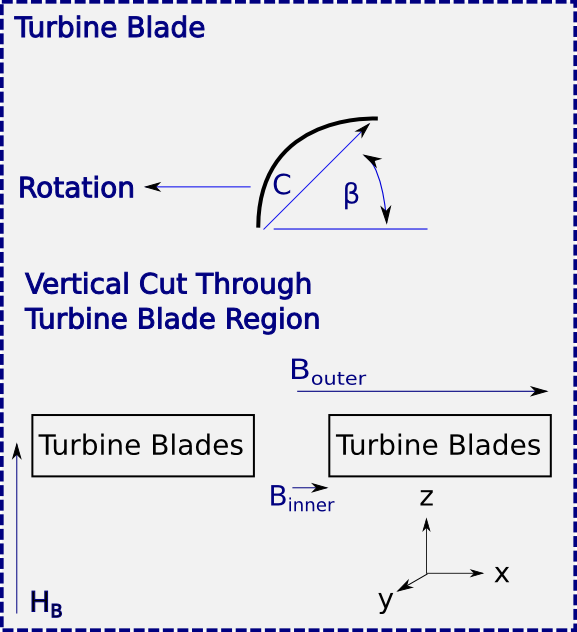
\includegraphics[width = 10 cm]{figs/turbine_image}
     \caption{The represented turbine blade
     geometry. $\beta$, the blade angle, is measured relative to the
     horizontal plane. c, the chord length of the turbine, is defined as
     the straight line distance from leading to trailing edge. } 
     \label{fig:turbine_image}
    \end{center}
  \end{figure}

\subsection{Drag Polar Specification}

We now define the lift and drag normals, where the direction opposing
drag is, by definition,  
\begin{equation}
{\bf n_{\text{drag}}} = \frac{{\bf u_p}}{||{\bf u_p}||} 
\end{equation}
and the direction opposing lift orthogonal to the drag and the radial 
direction,  
\begin{equation}
{\bf n_{\text{lift}}}= {\bf n_{\text{drag}}} \times {\bf n_r}. 
\end{equation}

Then, the force on the turbine is, 
% \begin{equation}
%  \boxed{F = \frac{1}{2}\frac{\rho u_p^2 c}{A}\left(C_l \cdot
% 					      n_\text{lift} + C_d \cdot
% 					      n_\text{drag}  \right)}
% \label{eq:force_turb}
  % \end{equation}
\begin{equation}
 F = \frac{1}{2} \rho A_B {\bf u_p}^2 \left(C_l 
					      {\bf n_\text{lift}} + C_d 
					      {\bf n_\text{drag}}  \right).
\label{eq:force_turb}
\end{equation}
$A_B$ is the total area of the turbine blades, so $A_B = B\, c\, r$, where B
is the number of turbine blades and c is the chord length of the
turbine. 
The actuator disk is an approximation of the blades as a volumetric
forcing ``disk'', and so our interest is in this quantity,
\begin{equation}
\frac{F}{\text{volume}} = \frac{F}{\pi r^2 t} = \frac{1}{2}\frac{\rho\, B\, c\,
 {\bf u_p}^2}{\pi r t}\left(C_l {\bf n_\text{lift}} + C_d {\bf
		   n_\text{drag}} \right).  
\label{eq:vol_turb}
\end{equation}
Where t is the blade thickness of the actuator disk.
Note that the volume is over a different extent than the area. The
volume is for the entire actuator disk, while the force on the blades
was only calculated with total surface area of the turbine. 
To better understand this, note that the product, $B c$ appears in
Equation~\ref{eq:vol_turb}, above. This quantity is a solidity (or
blockage) factor, and as the chord length or number of blades increases,
the total blocked area inside the actuator disk also increases. It is
interesting to note that in the actuator disk model, only this product
has impact, and one cannot directly separate the impact of more turbine
blades versus larger blade chord lengths. 
The impact of solidity will be discussed in greater detail in
Section~\ref{sec:solidity}.

Now, only the drag polars ($C_l,C_d$) must be specified to fully
determine the force on the blades. These drag polars are functions of
the angle of attack, $\alpha$. Plots of these drag polars were provided
by Duane McCormick at UTRC and were generated from a 2-D model in
COMSOL. As the data was discrete, high order polynomials were used
to obtain smooth functions fit to the COMSOL data. Typically,
16\textsuperscript{th} order polynomials were used to 
ensure that the fitted function closely matched the provided
data. The drag and lift functions for the three cases considered (flat
plates, $180^{\circ}$, $90^{\circ}$ circles) are shown in 
Figures~\ref{fig:flat_plate_drag}, \ref{fig:semi_drag} and
\ref{fig:90_drag}. The flat plate drag polars are smoothly
varying and so the interpolated function is close to the provided
data. The semi-circles ($180^{\circ}$) are largely accurate, but near
zero degrees the COMSOL data for the lift function shows a sharp feature
that is not well resolved by the interpolating polynomial. This is also
the case for the quarter-circles, where near a zero angle of attack the
lift function has a near discontinuity that is not well resolved by the
interpolated function. 

%The semi-circular plots are more complicated. Here, we use a high order
%polynomial fit to continuously interpolate between drag polars. 

\begin{figure}[!htb]
  \begin{center}
    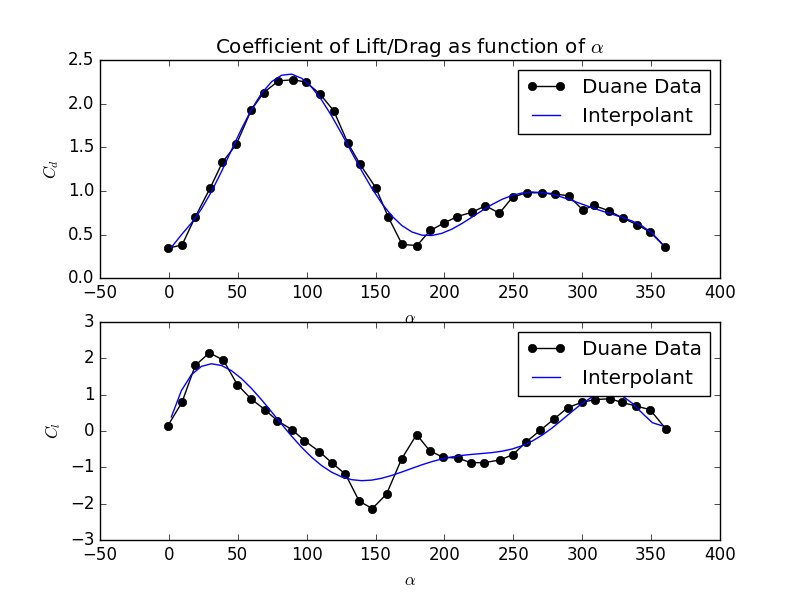
\includegraphics[width = 12 cm]{figs/flat}
    \caption{The flat plate drag polars.} 
    \label{fig:flat_plate_drag}
  \end{center}
\end{figure}

\begin{figure}[!htb]
  \begin{center}
    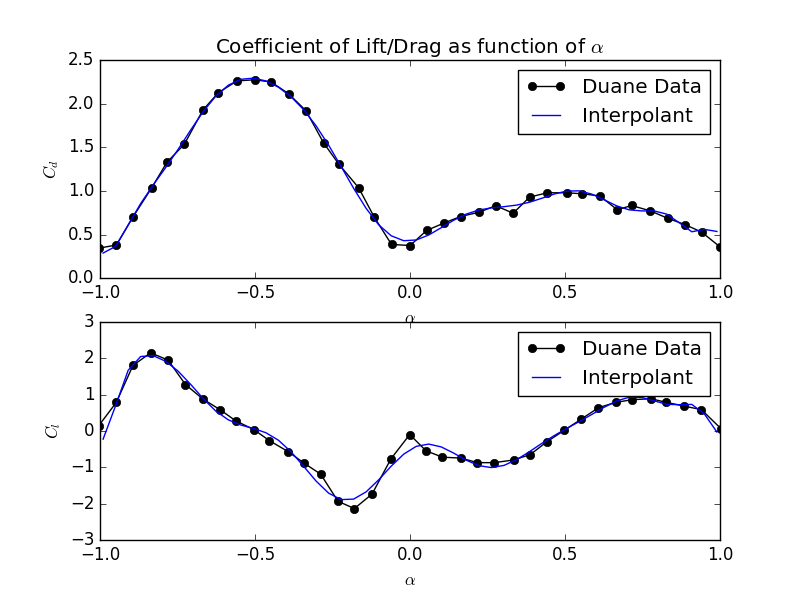
\includegraphics[width = 12 cm]{figs/semi}
    \caption{The semicircle (180 degree) drag polars.} 
    \label{fig:semi_drag}
  \end{center}
\end{figure}

\begin{figure}[!htb]
  \begin{center}
    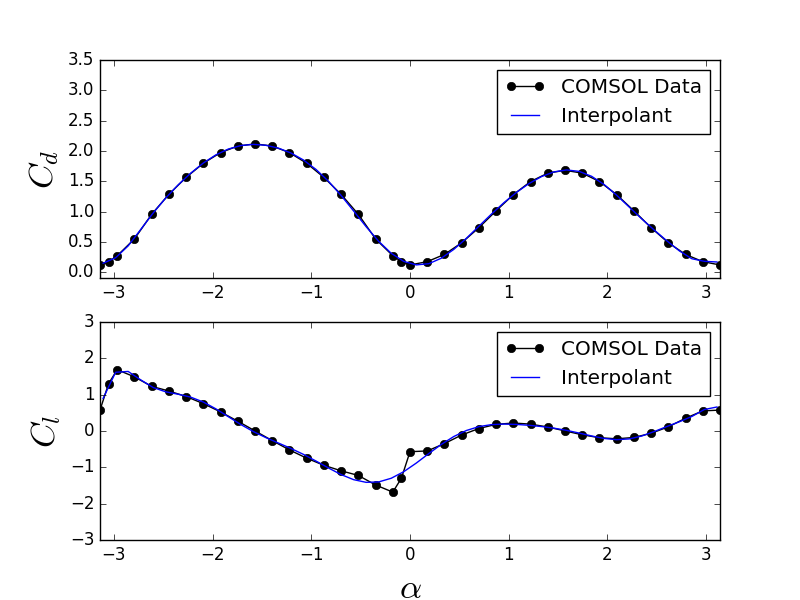
\includegraphics[width = 12 cm]{figs/90}
    \caption{The 90 degree drag polars.} 
    \label{fig:90_drag}
  \end{center}
\end{figure}

% what about loads on turbine?\todo{loads?}
% Blade torque loads modest, only ~20 ft-lbs
%% load was predicted at 20 ft*lbs

\subsection{Shortcomings of the Actuator Disk Model}
\label{subsec:wake_loss_model}

The actuator disk model is valuable because of its simplicity, not on
account of its accuracy. Despite its pervasive use, there are numerous
known inadequacies to the model. 

In particular, the actuator disk does not account for the separation of
flow between blades, and implicitly assumes the flow remains attached. 
This model deficiency results due to the actuator disk
method's dependence on the precision of the lift and drag
coefficients. During the operation of a wind turbine, should the angle
of attack reach high values (post-stall region), then aerodynamic
data is not available or inaccurate.  
This model inadequacy is commonly fixed with the Glauert Correction. 
Developed in 1926 by Glauert from helicopters rotor blades, this
correction originally was purely based on experimental data. The model
was designed to correct the overall thrust coefficient for high angles
of attack\cite{glauert1926general,glauert1935airplane}. 
While the Glauert correction is a tip loss model, the correction was
developed as a correction to an entire rotor disk; the original
researcher did not intend it to be applied to a rotor annulus. 
%Given that 
%a duct eliminates tip losses\todo{write me}
%However, because of a limited amount of experimental data, an alternative model does not exist.  

Nor do the model's described above account for the turbulent wake
state, which in some cases have been shown to be significant for a wind
turbine\cite{churchfield2012numerical} and may have substantial impact
on the SoV. 

Various researchers\cite{Moriarty_aerodyntheory,wilson1978design} have
suggested various other corrections to actuator-disk theory. These
corrections include (among others) accounting for blade thickness on
local angle of attack, cascade width for high solidity turbines, and
spanwise gaps for partial span pitch control. The impact of these
missing physics can be significant, for instance, blade thickness and
effects can be aerodynamically significant near the rotor hub and may 
affect the in-plane forces on the rotor. Nevertheless,
these corrections are not treated in the simulations presented in this
document. 

In summary, the actuator disk is a useful modeling tool for this study
but does not represent a high-fidelity representation of the turbine
blade dynamics, and should not be considered highly accurate. Attempts
to evaluate and characterize these shortcomings are detailed in
Chapter~\ref{sec:field}.  Additionally, a new modification to the
actuator disk that modifies the model to further account for blade
solidity is demonstrated in this work in Section~\ref{sec:solidity}. 

\section{Solid Surface Representation}
\label{subsec:solid_surface}

In addition to vanes, the SoV device includes impermeable surfaces
such as the wind break (``cone'') on the top of the facility. As with
the turning vanes, this is represented without explicitly meshing the
surface nor imposing  a boundary condition at the surface. This allows
rapid exploration of configurations  with different solid surfaces to
control and manipulate the fluid flow. These solid surfaces are
represented by a body force acting in a region surrounding the wall. 
A body force normal to the surface is defined in this region so
that it will drive the normal velocity to zero, resulting in the flow
moving only parallel to the virtual surface. 
The body force is defined as in Equation
\ref{eqn:body_force}; however, the length scale $\ell_v$ is specified to
be identical to the width of the surface being represented. This is
typically the width of two or three grid cells. While the actual surface we are
emulating is thinner than this, the numerical method has difficulty
converging for surfaces smaller than the grid size.  

Forcing models designed to mimic a surface
are not unique to this project, and the current formulation is
 closely related to (among others)
``immersed boundary methods'' as used by various other
researchers~\cite{doi:10.1146/annurev.fluid.37.061903.175743,verzicco1998complex}. This
approach is unique in its use of Babuska's penalty treatment of
constraints\cite{1973fempen,ZAMM:ZAMM19880680925} to enforce the
behavior at the boundary. This method was selected because it is easily
imposed in the FEM context, and the penalty method proper has been
explored in detail in the literature.
%\todo{add more discussion of
%healing length implications here} 

Note that despite the similarity in name, this is a distinct technique
from the ``penalty immersed boundary method'' of Kim and
Peskin\cite{:/content/aip/journal/pof2/19/5/10.1063/1.2734674}.  

%show image of cylinder in 2d flow?\todo{add cylinder image? what does
%zthis show?} 

%Typically, the enforcement occurs along a domain
%boundary, but in this work it is used in the interior, 
%and is not imposed as a mathematical constraint but rather as a modeling 
%approach. 

% We add a penalty term to the weak
% form of the Navier-Stokes momentum equation described in the subsequent
% section %\ref{eq:ns_weak} 
% that has the form, 
% \begin{equation}
% P_\epsilon = \int_\Omega ({\bf f_v} \cdot v) \, dx
% \end{equation}
% where ${\bf f_v}$ is as described in equation \ref{eqn:body_force}. 
%% As the system is formulated as a variational problem that seeks to
%% minimize the test function $v$, any velocity that is not aligned with
%% the vane normal will incur a penalty versus one that does. Note that unlike
%% some penalty methods, this does not automatically satisfy
%% continuity. Rather, the velocity field remains divergence free through a
%% separately enforced constraint.  

\section{Separation Model}
\label{sec:separation}

In the presence of wind, it was found that there was a significant flow
out through the vanes in the back of the device. This was obviously
inconsistent with the findings of our colleagues in the field, who
observed no outflows out of the back of the device. Moreover, this resulted
in large inconsistencies between our predictions and the field results,
almost certainly because of the kinetic and thermal energy that our vane
representation was permitting to leave out the back of the device.  

This exposed a weakness of the turning vane representation outlined
previously. When the flow entered the virtual vane forcing region it was
always turned to align with the vane angle, even when the forcing was in
the opposite direction of the present velocity.
This is in contrast to the physical situation, in which we
expect the flow to continue along an averaged streamline separating from the 
trailing edges of the vanes, instead of turning around it. 
The averaged streamline will continue past the trailing edge of the vane
due to the separation of the boundary layer off the edge surface. An
image depicting these two cases in shown in Figure \ref{fig:sep_model}.  

\begin{figure}[!htb]
  \begin{center}
    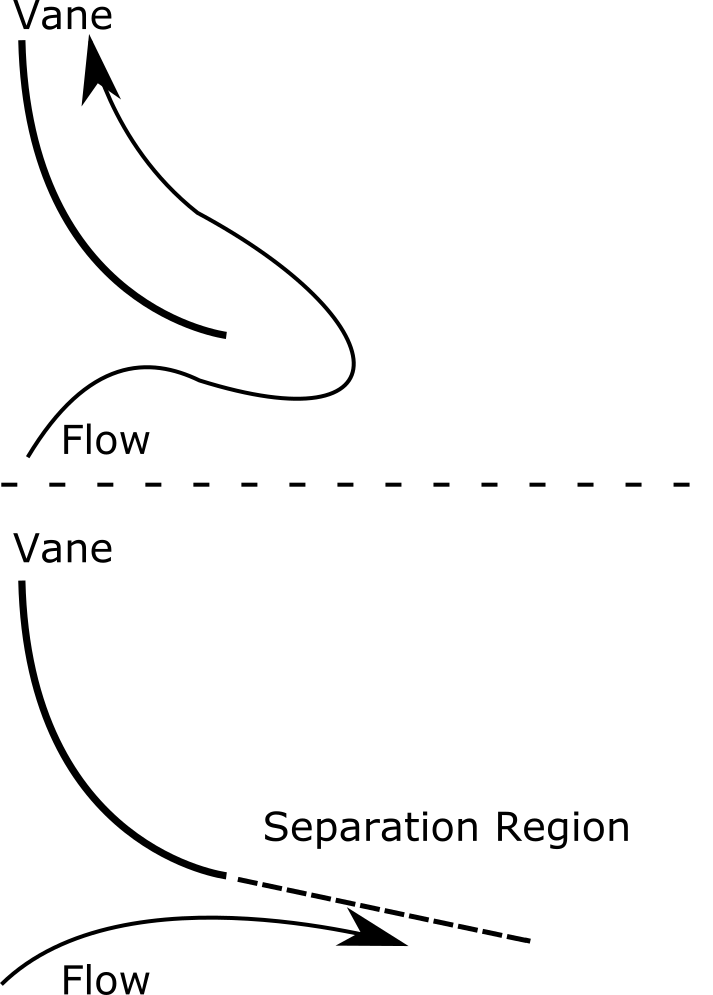
\includegraphics[width = 6 cm]{figs/sep_model}
    \caption{Schematic depicting the separation model that extends past
   the trailing edge of the vanes. In the top case, the flow entering
   the virtual vane region is forced to align with the vane angle despite
   this resulting in a reversal of the flow direction. This is a
   consequence of the forcing function acting on the fluid to ensure the
   velocity vector aligns with the vane. 
   The second case depicts the separation
   model, where the flow under certain conditions is not forced and
   continues to move tangent to the vanes due to 
   the separation of the boundary layer off the trailing edge.} 
    \label{fig:sep_model}
  \end{center}
\end{figure}

Let $\bf n_v$ be the normal vector to the vanes,
and $\bf n_r$ the normal vector pointing out of the vane
region\footnote{\normalsize The subscripts ``v'' and ``r'' stand for
vane and radial, respectively.}.  
Then, $\bf t_v$ is the tangential vector to the vanes pointing out of
the vane region and is defined as,

%\begin{equation}
% \bf t^v = \left( {\bf n^v_y},{\bf -n_x^v} \right) \text{sign}\left[
%	    \left( {\bf n^v_y},{\bf -n_x^v} \right) \cdot {\bf n^r} \right].
%\end{equation}
\begin{equation}
 \bf t_v = \left( {\bf n_v^{\perp}} \right) \text{sign}\left(
	    {\bf n_v^{\perp}} \cdot {\bf n_r} \right).
\end{equation}
Here, ${\bf n_v^{\perp}}$ is the vector perpendicular to the normal
vector of the vanes, which is simply, 
\begin{equation*}
 {\bf n_v^{\perp}} = \left[ \begin{array}{c}
n_x\\
n_y\\
\end{array}\right]^{\perp} = 
 \left[ \begin{array}{c}
  -n_y\\
  n_x\\
	\end{array}\right].
\end{equation*}

%
% example of an algorithm
%

\begin{center}
 \begin{algorithm}
  \caption{The crude separation model. This model identifies if the flow
  is coming into or out of the vane region, and if the velocity vector
  is in the same direction as the tangent line of the vanes. In the case
  of the ``special forcing'' the flow is forced as if it was
  impacting a solid surface. In the
  algorithm below, $r_0$ is the max radius of vanes, $r_i$ the minimum
  radius of vanes, and $\delta$ is the width of the separation region.}
  \label{alg:sep}
  \begin{algorithmic}
   \IF{($r_0 > r > r_i$)} 
   \IF{$(r_0 - r) < \delta$ \textbf{or} $((r - r_i) < \delta)$}
   \STATE ${\bf n_r} = {\bf r}/|r|$
   \IF{$(r - r_i) < \delta$} 
   \STATE ${\bf n_r} = -{\bf n_r}$
   \ENDIF
   \STATE  $\bf t_v = \left( {\bf n_v^{\perp}} \right) \text{sign}\left(
  	    {\bf n_v^{\perp}} \cdot {\bf n_r} \right)$
   \IF{$v \cdot t_v > 0$ \textbf{and} $v \cdot n_r < 0 $}
   \STATE ${\bf n}({\bf x}) = \hat r$ \quad (Special Forcing)
   \ELSE
   \STATE  ${\bf n}({\bf x}) = \sin \left(\phi(r) \right) \hat{{\bf r}}+ \cos
  \left(\phi(r) \right) \hat{{\bf \theta}} $
  \quad (Normal Forcing)
   \ENDIF
   \ELSE
   \STATE ${\bf n}({\bf x}) = \sin \left(\phi(r) \right) \hat{{\bf r}}+ \cos
  \left(\phi(r) \right) \hat{{\bf \theta}} $
  \quad (Normal Forcing)
   \ENDIF
   \ENDIF
  \end{algorithmic}
 \end{algorithm}
\end{center}


The forcing is modified when the velocity vector of the local flow, $\bf
u$ is pointing in to the forcing region: ${\bf u} \cdot {\bf n_r} < 0$, and
when the velocity vector is in the same direction as the tangent line to
the vanes: ${\bf u} \cdot {\bf t_v} > 0 $. In these instances, the
forcing acts as if there was a rigid surface past the vane edge, and
gives the appearance of a special ``no-penetration'' condition for the
velocity for these cases. The pseudo-code for this procedure is shown in
Algorithm~\ref{alg:sep}.

The addition of this simple separation model significantly reduced the
flow that penetrated the back of the vanes, and produces results
consistent with the observations provided by our experimental
colleagues.  

\section{Effect of Surface Roughness}

%%
%% this does not describe the phenomena being modeled or the precise
%% model -- rewrite
%%
%%
%% this does not say enough about the surface roughness
%% motivate that and explain how it is used, than show your estimate 
%% to argue it is small
%%

Surface roughness effects have been shown to play a role in the
formation of dust devils and related atmospheric
phenomena\cite{oke1987boundary}. For the flat and sandy
regions we are simulating, the impact is expected to be a small
``kick-up'' forcing velocity perturbation in the vertical
direction. Assuming azimuthal symmetry and forcing only inside the
region of the vanes ($r<R$), this is modeled as a volumetric forcing in
a narrow region above the surface,  
\begin{equation}
 F^{'''}_{z_0} = \frac{1}{2}\rho V_f^2/z_{0}, 
\end{equation}
where $z_{0}$ is the roughness height. We further assume that this
forcing is independent of ${\bf u}$. To estimate the magnitude of
$V_f$, we use a simple result from Newton's laws of motion,
\begin{eqnarray}
z_0 = \frac{1}{2} a t^2, \\
t = \sqrt{\frac{2 a}{z_0}}. \\
\end{eqnarray}
Combining this with, $V_f = a t$, our estimate is, 
\begin{equation}
V_f = \sqrt{2 a z_0}.
\end{equation}
The roughness height zero is set to the boundary layer thickness of 10
centimeters. The acceleration was estimated at 0.05
$\text{m}/\text{s}^2$, based on the observed surface roughness impact on
tornado-like vorticies of Natarajan and Hangan\cite{Natarajan2012577}.  

We ensure that the energy
introduced into the flow is a small fraction of total flow energy by comparing
this with the energy flux through the top of the vanes. The total energy
added is measured as,  
\begin{equation}
 E_{\text{injected}} = \int_0^{2\pi} \int_0^R \int_0^{z_0} F^{'''}_{z_0}
  dz dr d\theta.  
\end{equation}
R is the outer diameter of the vanes. 
The value of $E_{\text{injected}}$ is typically a few percent of the
total kinetic energy flux measured through the top of the
vanes.

Leslie~\cite{leslie1977surface} and Dessens~\cite{dessens1972influence}
found that the introduction of surface roughness effects caused a slight
decrease in tangential velocity for simulated vortices, but an increase
in radial and axial velocities. 
On a related note, hurricane studies have
consistently found enhanced heat transport near the surface lead
to storm intensification, indicating an important role due to roughness
effects~\cite{Zeng2010,GRL:GRL50047,hurricane_drag}. The interaction
with the surface and therefore, the impact of roughness, is likely
complicated and is not considered in detail in this work. It should be 
noted that in the simulations performed in the course of this study, the
surface roughness model was observed to modestly intensify the thermal
vortex, typically by several percent. While this formulation was
undoubtedly {\it ad hoc}, studies performed on representative test 
cases found that results were not sensitive to small
changes in the forcing region height, radial distance, or
forcing magnitude. 

%This general forcing provides additional capabilities including the
%ability to investigate engineering greater surface roughness or
%structures that could provide greater ``kick-up'' of the thin thermal
%layer near the surface into the flowing regime. It can also support more
%general turning configurations than the virtual vanes outlined above. 

\section{Simulation Geometry and Boundary Conditions}
\label{sec:bc}

In this project, two principle modeling regimes are considered.  
One is the ``thermal-only'' scenario, in which there are no ambient
velocities and there is an imposed elevated temperature on the ground.  
In the other, there are also ambient winds that contribute to the SoV energy
(``wind'' cases). 
The computational domain and boundary conditions for these 
two scenarios are described below.

%\subsection{Computational Domain} 
\textbf{Computational Domain} 

All simulations are performed in a cuboid domain, with six
faces.  The domain is denoted $\Omega \subset \mathbb{R}^3$. 
The domain extents are scaled by the system diameter, D, created by the
outer vane radius. The extents are defined in terms of $\{L_x,L_y,L_z\}$ indicating the 
streamwise, spanwise and vertical directions, respectively. 
For both simulation regimes, sensitivity analyses 
were performed to ensure that the results were not sensitive 
to the domain extents. For the thermal-only case, for which $L_x = L_y$,
the system 
extents $L_x/D$ and $L_y/D$ are chosen to be 3. The height ($L_z/D$) is
three times the system diameter, which is typically nearly equal to the
height of the vanes. This defines the thermal-only domain $\Omega_T$, 
as $\Omega_T = \left[-L_x,L_x \right] \times \left[-L_y,L_y \right]
\times \left[0,L_z \right]$.   

For the wind cases, the streamwise extent is no longer equal to
the spanwise length, $L_y$. In these cases, the domain length extends
two diameters in front of the vanes and three behind. The
spanwise direction is symmetric and extends two diameters in each direction 
from the center ($L_y/D = 2$). The height is identical to the
thermal-only case, at three system diameters ($L_z/D = 3$). Thus, the
wind domain is defined as $\Omega_W = \left[-2D,3D \right] \times
\left[-L_y,L_y \right] \times \left[0,L_z \right]$.   

The boundary for the thermal only case is decomposed as,
$\partial \Omega_T = \Gamma_G \, \bigcup \, \Gamma_T \, \bigcup \, \Gamma_P $. 
$\Gamma_G$ is the boundary along the ``Ground'', $\Gamma_T$
the ``Top'' boundary, and $\Gamma_P$ the four periodic ``Sides''. A 3d
diagram labeling these boundaries is shown in
Figure~\ref{fig:thermal3d}. For this case study (no mean wind),
periodic boundary conditions are used on the four sides , with a modified 
``inflow-outflow'' Neumann condition\cite{gunzburger1989finite} on the
top boundary. On the ground, a ``no-slip'' velocity boundary condition is
imposed, and a Dirichlet condition uniformly fixes
the temperature of the surface. 
Each of the $\Gamma$ boundary terms are defined in the paragraphs below. 
Note that a finite thickness ``Sponge Layer'' is
indicated on the figure along the top boundary and is defined below. 

\begin{figure}[!htb]
  \begin{center}
    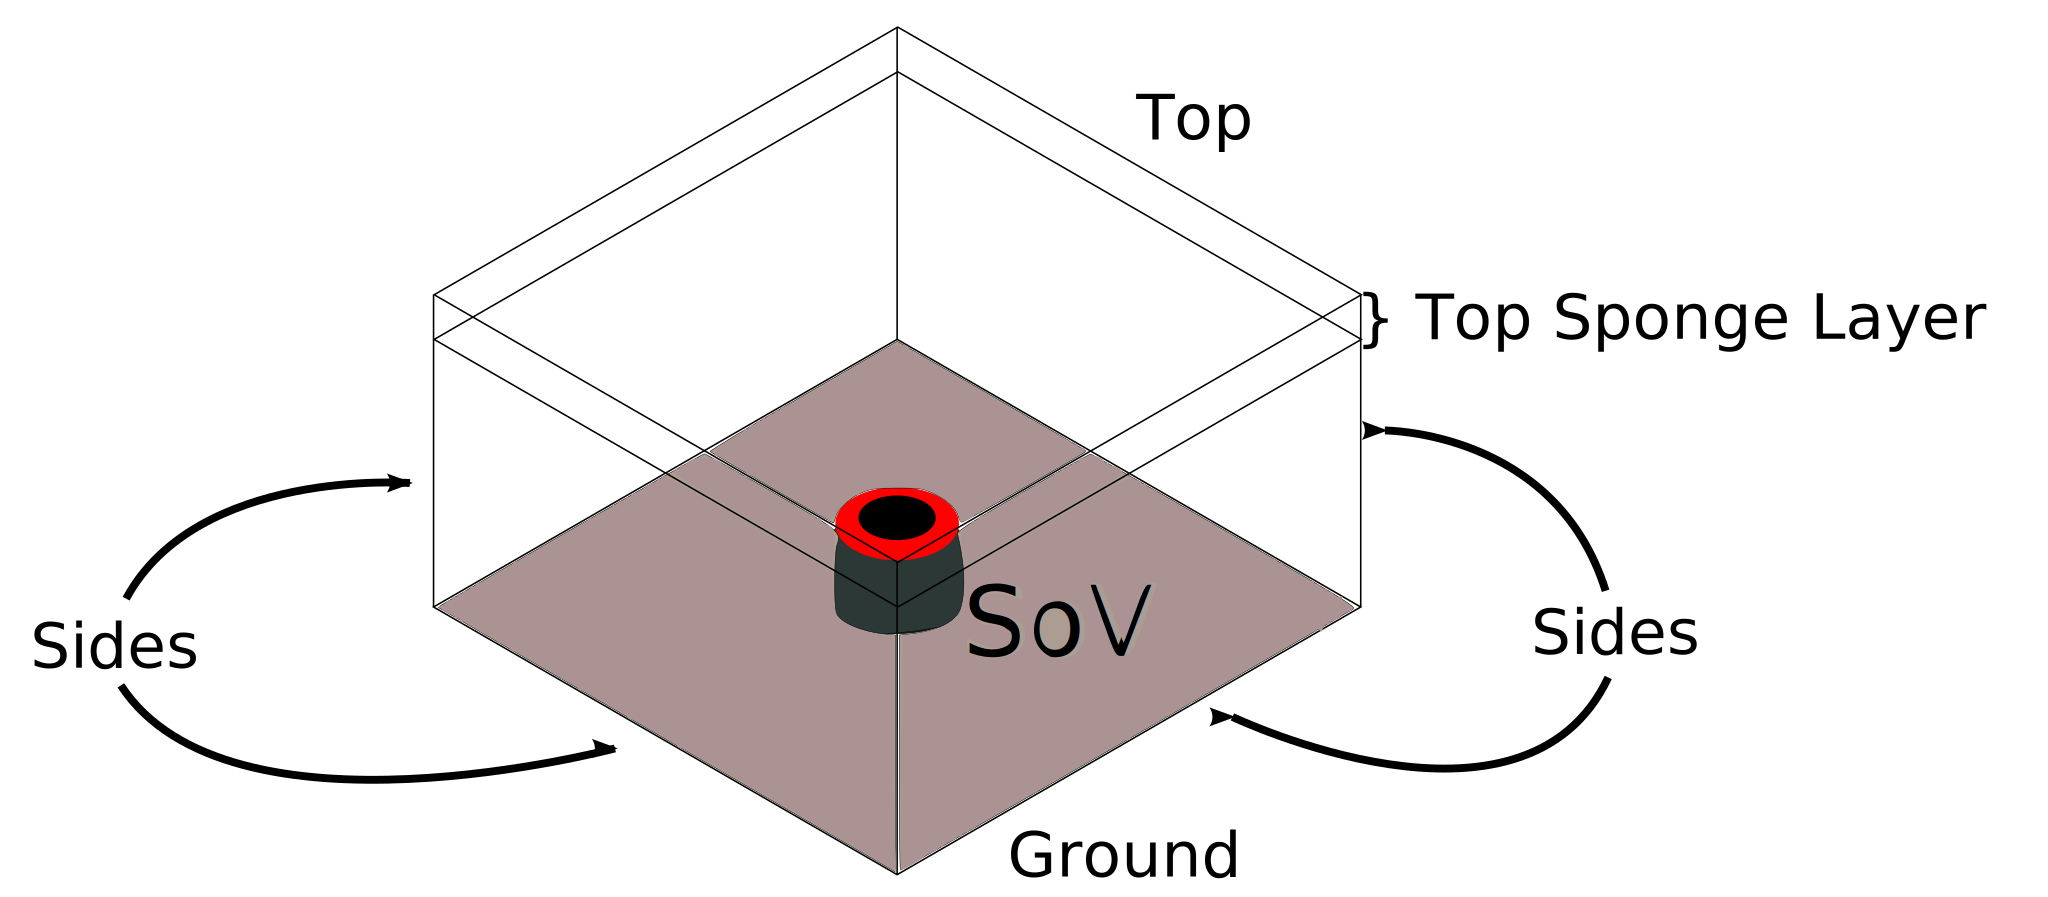
\includegraphics[width=14cm]{figs/thermal_only_3d}
    \caption{Domain for the thermal-only
   scenario. The diagram scale is representative of typical cases. Note
   the SoV apparatus in the center, which provides perspective on the
   extent of the domain with respect to the turning vane diameter. The
   ground, sides and top boundaries are labeled with the discussion the
   precise boundary conditions on each provided in
   Section~\ref{sec:bc}. Notice also the finite thickness, high
   viscosity ``sponge layer'' at the top of the domain.} 
    \label{fig:thermal3d}
  \end{center}
\end{figure}

The boundary for the wind cases is decomposed as,
$\partial \Omega_W = \Gamma_G \, \bigcup \, \Gamma_T \, \bigcup \,
\Gamma_O \, \bigcup \, \Gamma_I \, \bigcup \, \Gamma_S $.  
Where $\Gamma_G$ is the boundary along the ``Ground'',
$\Gamma_T$ the ``Top'' boundary, $\Gamma_S$ the two ``Sides'',
$\Gamma_I$ the inflow boundary, and $\Gamma_O$ the ``Outflow''  
boundary.
The ``wind'' simulation domain is diagrammed in
Figure~\ref{fig:wind3d}, with the boundaries labeled. 
For this particular study (a heated ground with 
an ambient wind), the wind case has a proscribed inlet boundary layer
along the upstream streamwise face ($\Gamma_I$) for both the temperature
and the velocity. The ``Ground'' boundary is identical to
the thermal-only case. The ``Sides'', ``Outflow'' and ``Top'' are all
set to modified Neumann boundary conditions. Note that ``Sponge Layers''
are used on both the back boundary and the top. 

\begin{figure}[!htb]
  \begin{center}
   \includegraphics[width=14 cm]{figs/wind_3d}
    \caption{Domain for the wind and thermal scenario. The diagram scale
   is representative of typical cases. Note the SoV apparatus which
   provides perspective on the extent of the domain with respect to the
   turning vane diameter. The ground, sides, inflow, back and top
   boundaries are labeled with the discussion the precise boundary
   conditions on each provided in Section~\ref{sec:bc}. Notice also the
   finite thickness, high viscosity ``sponge layer'' at the top and back
   of the domain.}   
    \label{fig:wind3d}
  \end{center}
\end{figure}

\textbf{Ground Boundary Conditions, $\Gamma_G$} 

For both the wind and thermal-only cases the ground has a fixed
temperature and no-slip velocity boundary conditions. This boundary 
($\Gamma_G$) is modeled with a Dirichlet boundary condition, 
\begin{align}
 {\bf u} &= 0 \quad \text{ on } \Gamma_G \\
 T &= T_g.
\end{align}
Where $\Gamma_G = \{(x,y,0) \subset \partial \Omega \} $. 

%
% http://fenicsproject.org/documentation/dolfin/dev/python/demo/documented/periodic/python/documentation.html 
%
%
\textbf{Periodic Boundary Condition, $\Gamma_P$} 

A periodic boundary condition is used in the thermal only cases, 
along the streamwise and spanwise boundary faces 
(denoted $\Gamma_{P,x}$ and $\Gamma_{P,y}$, respectively). In these
cases the state variables  
are contrained to have the same value on the opposite faces of the domain, 
for instance in the streamwise direction the boundary conditions are, 
\begin{align}
 {\bf u}(-L_x,y,z) &= {\bf u}(L_x,y,z) \quad \text{ on } \Gamma_{P,x} \\
 T(-L_x,y,z) &= T(L_x,y,z)
\end{align}
and in the spanwise direction,
\begin{align}
 {\bf u}(x,-L_y,z) &= {\bf u}(x,L_y,z) \quad \text{ on } \Gamma_{P,y} \\
 T(x,-L_y,z) &= T(x,L_y,z). 
\end{align}
Where $\Gamma_{P,x} = \{(-L_x,y,z) \, \bigcup \, (L_x,y,z) \subset \partial
\Omega \}$  
and $\Gamma_{P,y} = \{(x,-L_y,z) \, \bigcup \, (x,L_y,z) \subset \partial
\Omega \}$. 

\textbf{Inflow Boundary Condition, $\Gamma_I$} 

On the inflow boundary $(\Gamma_I$), dirichlet conditions are used for both
velocity and temperature. The boundary-normal, or streamwise component 
is a function of the surface normal coordinate (z), representing a boundary 
layer below a uniform velocity, U.
The common 7th power model of a turbulent boundary layer is used,   
\begin{equation*}
  u_{\text{in}}(z) = U \text{ min }\left(\left(\frac{z}{\delta}\right)^7,1\right)
  \label{eq:bl_u}
\end{equation*}
where $\delta$, the boundary layer thickness, is set based on data
measured by our experimental partners in the field. 
The thermal boundary layer is assumed to have a similar boundary layer,
but, as observed in real atmospheric flows, there remains a vertical
temperature gradient outside the thin boundary layer. Based on
results in the literature a $2/3$ Kelvin per meter gradient is 
imposed\cite{Blocken2007238}. The thermal inflow is then  
\begin{equation*}
  T_{\text{in}}(z) = \Delta T \left(1- \text{ min
			}\left(\left(\frac{z}{\delta}\right)^7,1\right)\right)
  + T_0 - 2z/3.  
  \label{eq:bl_t}
\end{equation*}
% 335+18*tanh(-z/0.1)-z*2/3
The inflow boundary is at the surface $x=-L_x$.

\textbf{Mixed inflow/outflow Boundary Conditions on $\Gamma_T$,
$\Gamma_S$ and $\Gamma_B$}  

At outflow boundaries, a homogeneous ``do nothing'' Neumann condition is
appropriate\cite{Rannacher2000}, 
\begin{align}
  \frac{\partial u}{\partial n}\bigg|_{\Gamma_T} = 0 \\
  \frac{\partial T}{\partial n}\bigg|_{\Gamma_T} = 0
\end{align}
However, for the cases in this study, a modified Neumann condition is
necessary due to the possibility that there will be an inflow on these
boundaries. 
For example, in the region above the vanes, the concentrated hot plume is
lifted by buoyancy upward and out of the simulation domain. However, the
radial inflow towards the apparatus is drawn in by large scale
convection cells larger than the system diameter. Thus, our boundary
conditions must permit inflow along the areas above and external to the
vanes, while simultaneously permitting outflow in the area above the vanes. 

% Roy Stogner: Okay, so this DDN is basically no-traction when there's 
% outflow and Tn=v when there's inflow?  We have no-traction for v*n, 
% no-traction for anything else when there's outflow, and Dirichlet
% v.cross.n = 0 when there's inflow. 

To accomplish this, the boundary condition is,
\begin{align}
  \frac{\partial u_n}{\partial n}\bigg|_{\Gamma_T} = 0 \\
  \text{if } (w<0) \text{ then}& \begin{cases}
    u_t = 0,\\
    T = T_{\text{in}}
  \end{cases} \\
  \text{ else}& \begin{cases}
    \frac{\partial u_t}{\partial n}\bigg|_{\Gamma_T} = 0, \\  
    \frac{\partial T}{\partial n}\bigg|_{\Gamma_T} = 0
  \end{cases}
\end{align}

where $u_n$ and $u_t$ are normal and tangential components of the velocity, 
respectively. This boundary condition is applied on the top boundary
$\Gamma_T$ ($z=L_z$) and downstream side boundary  $\Gamma_B$ in the
wind case. This mixed boundary condition appears to be a unique
implementation of a ``directional do-nothing'' condition, which has been
demonstrated previously in other
instances~\cite{braack2014directional,feistauer2006non}. In particular,
the well-posedness of this general class of boundary condition is
treated in \cite{bruneau1996new}.  

\textbf{Sponge Layer} 

Finally, a finite thickness ``sponge layer'' is used in the region adjacent 
to the mixed inflow/outflow boundaries $\Gamma_T$ and $\Gamma_B$.
These regions are referred to by many names in the
literature\cite{doi:10.1146/annurev.fluid.36.050802.121930}, such as
absorbing layers, fringe regions, buffer zones, sponges,
etc. 
This layer artificially increases the momentum diffusivity by
a factor of ten times the nominal value. This was designed to stabilize
the modified Neumann boundary conditions which can exhibit an instability
when there is a compact jet of fluid leaving the domain. 
These small outflows would create small high velocity inflows, and the
feedback loop would result in instabilities and numerical
blow-up. Mindful of the fact that the character of solution not
important in this region, and that our physical interest remains focused
on the region inside and in immediate proximity to the vanes, we
introduced a higher diffusivity ``sponge'' region that would diffuse the
high velocity exiting jets sufficiently to prevent numerically
un-physical behavior. No results are quoted from this ``sacrificial''
region, as it is not considered physically meaningful. The top sponge
layer in both the wind and thermal-only cases are set to be half a
system diameter $(L_z/D = 1/2)$. For the wind cases, the back sponge
layer is also set to be half a system diameter $(L_x/D = 1/2)$. 

%\todo{expand this? how thick did it need to be?}


\chapter{Computational Methods and Software}
%\section{Computational Methods and Software}
\label{sec:software}

The previous chapter described a set of models 
for the system of interest. 
%These models are too 
%complicated to solve exactly, and must instead be 
%instantiated with software to produce a numerical 
%result. 
This chapter details the numerical formulation
and simulation of these models. It begins with a 
discussion of the numerical discretization of the equations 
of interest. The mesh discretization is then described. 
Next, the scientific software in which these numerical 
models are used is discussed. Finally, the tool
chain and supercomputer systems are briefly introduced. 

\section{Discretization Scheme}
\label{sec:discretization}
The finite element method (FEM) is used to numerically solve the 
Navier-Stokes equations on a computer. The starting point for the FEM is
to cast the equations in section~\ref{sub_sec:ns_en} into a weak
form. A weak form is used to reduce the continuity requirements on the
basis functions, thereby allowing the use of functions that are
easy to construct and implement, such as piece-wise polynomials. 
Manipulating these partial differential equations into a
variational formulation is accomplished by multiplying the equations by
appropriate test functions and integrating over the domain,
$\Omega$. The resulting weak problem is: find $({\bf u},p,T) \in
H^1(\Omega)^3 \times L_2(\Omega) \times H^1(\Omega)$ such that 

%
% http://www.numerik.uni-hd.de/Oberwolfach-Seminar/CFD-Course.pdf
%
\begin{align}
  (\frac{\partial{\bf u}}{\partial t},{\bf v}) + ({\bf u} \cdot \nabla{\bf
 u},{\bf v}) + \nu (\nabla{\bf u}, \nabla{\bf v})   
  -(p,\nabla \cdot{\bf u}) &= ({\bf g} \, T'/T_0,v)
 \label{eqn:ns_weak} \\
 (\nabla \cdot{\bf u},q) &= 0
 \label{eqn:cont_weak} \\
 (\frac{\partial T}{\partial t}, w) + ({\bf u} \cdot \nabla T,{\bf
 w}) + (k \, \nabla T, \nabla  w) &= 0.\label{eqn:en_weak}
\end{align}

$\forall ({\bf v},q,w) \in H^1(\Omega)^3 \times L_2(\Omega) \times
H^1(\Omega)$, where $(\cdot,\cdot)$ denotes the $L_2$ inner product, 
$(u,v) = \int_\Omega u \cdot v \, dx$ and $H^1(\Omega)$ is the
Sobolov space with one square integrable derivative on the domain
$\Omega$\cite{oden2012introduction}. As noted previously, boldface letters
denote vector quantities (such as ${\bf u} = \left \{ u,v,w \right \}$). 
Some of the simulations presented here were conducted under
steady conditions, for which the $\frac{\partial}{\partial t}$ terms
vanish. An FEM scheme is obtained by posing the weak form in
terms of discrete subspaces of the function spaces specified above
defined using piecewise-polynomial basis functions. This discretization
has the form, $ {\bf v_h} \in {\bf v}$, where ${\bf v_h}$ is an
approximation of ${\bf v}$ formed through a linear combination of a
finite number (N) of terms,  
\begin{equation}
 {\bf v_h} = \sum_{i=1}^N \alpha_i \phi_i,
\end{equation}
where $\alpha_i$ are constants and the N basis functions, $\left \{
\psi_1, \psi_2, \ldots, \psi_N \right \}$, define an N-dimensional 
subspace of $H^1$\cite{becker1981introduction}. All of the simulations
discussed in this work were 
accomplished using linear basis functions for both the velocity and
pressure. Typically, the use of equal order elements for velocity and
pressure is ruled out in the standard Galerkin FEM formulation by the
Babuska-Brezzi condition\cite{bb-cond}. 
However, the weak form equations shown above are stable with equal-order
elements for velocity and pressure due to the introduction of pressure
stabilization terms. The resulting system is still open to convective
instabilities, and so streamline upwind/Petrov-Galerkin (SUPG)
stabilization terms are used, as first described by
Hughes\cite{Hughes198685,supg} and extended to natural convection as in
Becker and Braack\cite{Becker2002428}. These stabilization terms add 
a residual dependent artificial dissipation that approaches zero as the
residual converges. This scheme is called ``consistent'' because the
underlying order of convergence of the numerical method is not
affected\cite{hughes2000finite}.   

The stabilization described above is accomplished by introducing an additional term,
$\langle L{\bf c},S {\bf \phi} \rangle_\tau$, to the weak form defined in Equations
\ref{eqn:ns_weak}-\ref{eqn:en_weak}. Here $L()$ is the operator for the PDEs
in \ref{sub_sec:ns_en}, and S() is a stabilization operator
which is chosen to be the negative adjoint of the differential operator
terms of $L()$, and ${\bf c}$ and ${\bf \phi}$ are state and test
function vectors, i.e. $ {\bf c}= ({\bf u},p,T)$, and ${\bf \phi} = (
{\bf v},w,q )$. The angle brackets $\langle \cdot,\cdot \rangle$ signify
integration of the element interiors for each of the K elements, that is:
\begin{equation}
 \langle {\bf u},{\bf v} \rangle_\tau = \sum_K \tau_K({\bf u},{\bf v})_K.
\end{equation}
This results in three stabilization parameters, $\tau_P, \tau_v, \tau_T$ 
which are selected as proposed by Becker and Braack. 
A full derivation of the weak form and stabilization terms are provided
in Appendix \ref{app:stab}. 

After spatial discretization, the system of ODEs are discretized in time
using the backward Euler method\cite{moin2010fundamentals}. The time
interval $(0,T)$ is sliced into $N_t$ steps of uniform temporal length,
$\Delta t$, where $n = 0,\dots,N_t$.  
This has the form, 
\begin{equation}
 {\bf y}_{n+1} = {\bf y_n } + \Delta t \, f({\bf y_{n+1}},t_{n+1}).
\end{equation}
Where ${\bf y_{n+1}}$ denotes the solution vector at the time step $n+1$, for
instance. As $f$ is non-linear, a Newton-Raphson method is used to solve
the resulting implicit nonlinear problem. While an iterative method is
significantly more computationally expensive per timestep than a similar
explicit method, the method was selected due to its unconditional
stability and ease of statistical sampling for a uniform timestep.  

%
% gave not completely described numerical methods
% for instance, have not indicated the stabilization schemes
% do not need complete equations, but should permit someone to access 
% the literature and construct precisely the numerical formulations used
%


\section{Mesh Discretization}

%
% what about mesh...
%
The domains described in section~\ref{sec:bc} are
consistently discretized. The domain extents
are scaled by system diameter but the same number of grid points are used
for every simulation. Thus, while the ratio of the domain length to system
diameter remains fixed, the grid spacing increases proportionally with
domain length. 

The mesh has a uniform spacing in the lateral directions, except for a
single refinement in the region of the vanes. Typically, the grid is 
roughly one hundred points in the streamwise and spanwise directions
before the refinement. The refinement halves the spacing (doubles the
number of points) in all three
coordinate directions, \{x,y,z\} in this region. The refinement is made
from the ground to 1.5 times the height of the vanes and cone. 

The mesh is non-uniform in height to
resolve the boundary layer. This is accomplished by redistributing a
mesh uniform in height, z, according to,
\begin{equation}
 z = \begin{cases} C_1(z-L_z)+L_z,& \text{if } z \geq z_\delta\\
      C_2 \text{ exp}(C_3 z - 1),                 & \text{otherwise}
     \end{cases}
\end{equation}

where $z_\delta$ is the chosen height of the boundary layer mesh, and
$C_1-C_3$ are scaling coefficients\todo{show coefficients}. 
This gives the mesh an exponentially
varying character, with the coefficients chosen to ensure ten or more
points in the boundary layer, isotropic spacing in cells outside of
it, and smooth blending between these two regimes. Each boundary layer
spacing was tested against a finer spacing to ensure that the results
were not sensitive to the choice of spacing. A horizontal slice though a
representative domain is shown in Figure \ref{fig:meshing}. The single
refinement in the region of the vanes is visible, along with the finer
meshed boundary layer region near the ground. 

  \begin{figure}[!htb]
    \begin{center}
     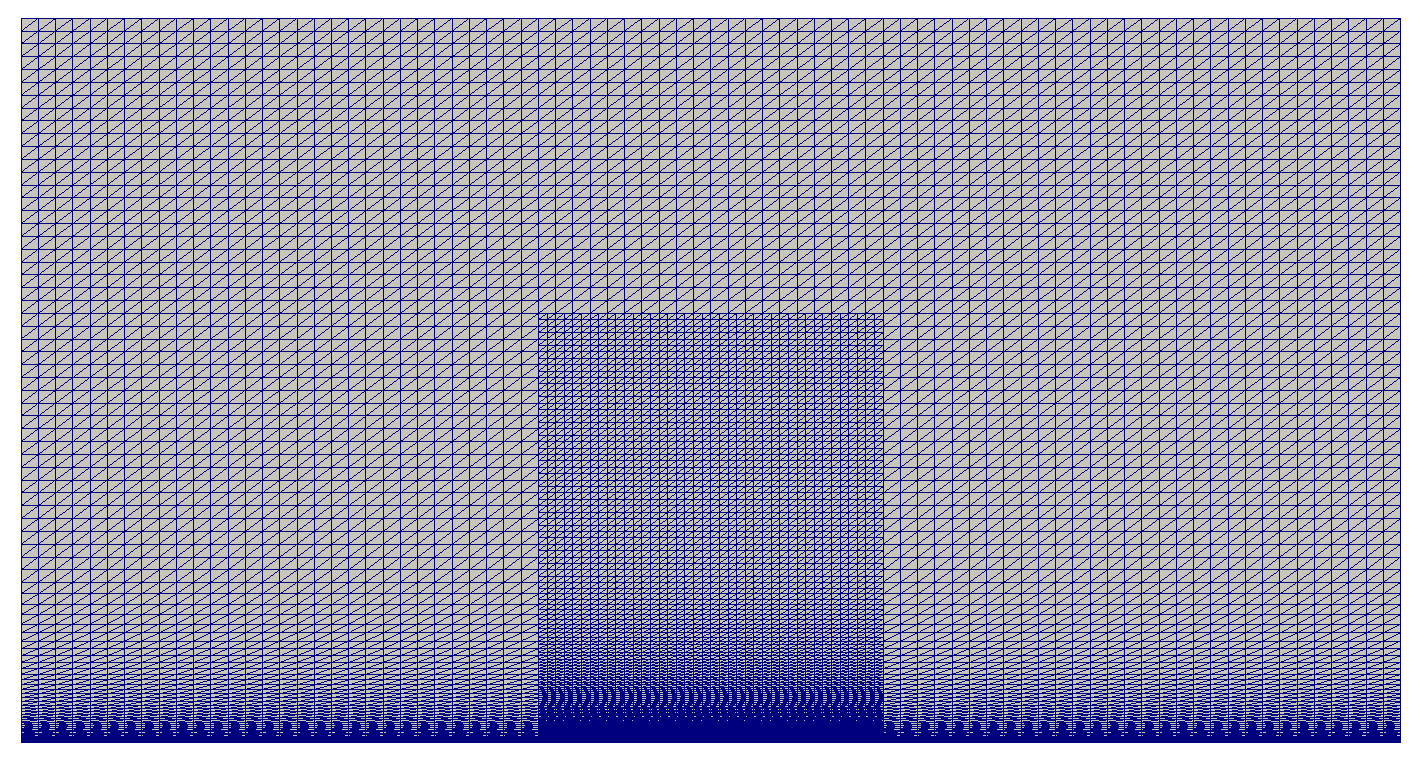
\includegraphics[width = 10 cm]{figs/meshing}
     \caption{Horizontal slide through the domain, to show a
     representative meshing. The single refinement region around the
     vanes is visible, along with the finer boundary layer mesh near the
     ground.}
     \label{fig:meshing}
    \end{center}
  \end{figure}

Finally, the diffusivities are proportionally
scaled with grid size to ensure that the cell Reynolds number, 
\begin{equation}
 \text{Re}_\text{cell} = \frac{\text{max}(\Delta x,\Delta y) u}{\nu_T}
\end{equation}
 is maintained for every simulation, to ensure stability.


%% hmin = 0.001  
%% hmax = 0.4  
%% zb = 2.0
%% hrat = ${/ ${mesh-options/hmax} ${mesh-options/hmin}}
%% zmax = ${mesh-options/domain_x3_max}
%% loghrat = ${= log ${mesh-options/hrat}}
%% c2 = ${/ ${mesh-options/zb} ${- ${mesh-options/hrat} 1}} 
%% zetab = ${/ ${mesh-options/zmax} ${+ 1 ${/ ${- ${mesh-options/zmax} ${mesh-options/zb}} ${* ${mesh-options/c2} ${mesh-options/hrat} ${mesh-options/loghrat}}}}}
%% c3 = ${/ ${mesh-options/loghrat} ${mesh-options/zetab}}
%% mesh_nx3 = ${= ceil ${/ ${* ${mesh-options/zmax} ${mesh-options/c2} ${mesh-options/c3}} ${mesh-options/hmin}}}
%% c1 = ${* ${mesh-options/c2} ${mesh-options/c3} ${= exp ${* ${mesh-options/c3} ${mesh-options/zetab}}}}
%% redistribute = '{x}{y}{if(z>${mesh-options/zetab},${mesh-options/c1}*(z-${mesh-options/zmax})+${mesh-options/zmax},${mesh-options/c2}*(exp(${mesh-options/c3}*z)-1))}' 

%After operation, solutions are evaluated to ensure that 
%the qualitative character of the solution does not change.

\section{Software Stack}

The numerical formulations described in Section~\ref{sec:discretization}
had been implemented using the GRINS library\cite{GRINSpaper} by Bauman
and Stogner using the Libmesh\cite{libMeshPaper} FEM infrastructure. It
was designed to support multiphysics FEM applications, the reusability
and extensibility of mathematical modeling kernels, supporting
interfaces to existing solver and discretization libraries to enable
modern solution strategies, while, at the same time, retaining
flexibility to effectively address a wide range of science and
engineering problems.   

GRINS provides a platform that enables powerful numerical algorithms
such as adjoint-based AMR, adaptive modeling, sensitivity analysis,
and, eventually, enabling uncertainty quantification. While few of these
capabilities are in use for the present work, they could be useful in
future investigations. 

GRINS stands for, ``General Reacting Incompressible Navier-Stokes'',
which roughly encapsulates the physical regimes it was originally
designed to simulate. GRINS is open-source, and available on
\hyperref[www.github.com/grinsfem/grins]{GitHub}. It is released 
under LGPL2.1.  GRINS is heavily unit tested, with over 60 tests
available to ensure the reliability of results regardless of install
platform. 

%The remainder of this section is devoted to
%discussing the underlying libraries used and the description of the
%GRINS framework.  

GRINS uses the fparser\cite{fparser}
library to support both parsing and compilation of mathematical
functions into high performance kernels. This capability allows for
easy specification of boundary conditions, initial conditions, or
constitutive equations from an input file. Some of these inputs are
detailed in Appendix~\ref{sec:archiving}. 

GRINS/Libmesh are built on the PETSC\cite{petsc} solver package, which
provides the numerical linear algebra packages used for constructing and
using sparse matrices, finding the iterative solution of linear systems,
and for preconditioning.  

While a variety of solver options have been tested in PETSC, all the
results shown in this document use GMRES with block Jacobi for
preconditioning\cite{Saad:2003} for the linear solve. This uses the
inverse of the diagonal block for that processor for preconditioning of
the entire linear system. In addition, a preconditioner is used for the
solution of the diagonal block. This is approximated with incomplete LU
factorization\cite{?}. Here, the ``incomplete'' refers
to the level of fill you use, with greater levels of fill approaching
the ``complete'' LU factorization. 

In principle, alternative software libraries/frameworks such as
FEniCS\cite{fenics}, OpenFOAM\cite{openfoam}, etc. would likely be
capable of simulating this regime. While these and other libraries have
various strengths and weaknesses, the pre-eminent concern is the parallel
performance at the intended processor count, due to the rapid
design iterations necessary for this research campaign. Given these concerns,
the GRINS library is a satisfactory tool. 

%% (11:41:54 AM) nick: ``-ksp_view -ksp_type gmres -pc_type bjacobi
%% -sub_pc_type ilu -sub_pc_factor_levels 0'' 
%% (11:42:00 AM) Paul Bauman: OK
%% (11:42:17 AM) Paul Bauman: -pc_type is the preconditioner for the entire linear system
%% (11:42:25 AM) Paul Bauman: You're doing bjacobi = block Jacobi
%% (11:42:28 AM) nick: right
%% (11:42:36 AM) nick: and does anyone have a good reference I can learn
%% this better? i feel as if I cant look this up, for some reason 
%% (11:42:39 AM) Paul Bauman: That is just using the inverse of the
%% diagonal block for that processor 
%% (11:42:46 AM) Paul Bauman: Now
%% (11:42:55 AM) Paul Bauman: that is a linear solve
%% (11:43:17 AM) Paul Bauman: So you can use all the linear solver
%% technology to solve or approximately that block 
%% (11:43:24 AM) Paul Bauman: Hence, -sub_pc_type
%% (11:43:32 AM) hil left the room.
%% (11:43:46 AM) Paul Bauman: That's the preconditioner it's going to
%% use to precondition the linear system for the solution of the
%% diagonal block 
%% (11:43:53 AM) Paul Bauman: You're telling it to use incomplete lu
%% (11:44:26 AM) Paul Bauman: Now the -sub_pc_factor_levels options
%% applies to ilu 
%% (11:44:28 AM) hil entered the room.
%% (11:44:44 AM) Paul Bauman: The incomplete part of imcomplete LU is
%% about the level of fill you use 
%% (11:45:05 AM) Paul Bauman: The more levels of fill you have, the more
%% ``complete'' the incomplete LU will be 
%% (11:45:08 AM) Paul Bauman: Does that make sense?
%% (11:45:23 AM) nick: no, that is where you lost me
%% (11:45:39 AM) nick: i dont think i know this level of fill
%% (11:46:17 AM) Paul Bauman: Check out Youssef Saad's book if more
%% curious about the subject 
%% (11:46:37 AM) nick: cool thanks
%% (11:46:38 AM) Paul Bauman: Suffice it to say, you heopfully shouldn't
%% ever need to go past 3 or 4 levels of fill 
%% (11:47:03 AM) Paul Bauman: Also, if you've got superlu installed with
%% the PETSc, consider using -sub_pc_factor_mat_solver_package superlu 
%% (11:47:15 AM) Paul Bauman: That's a *much* faster/better
%% implementation than PETSc's 

At the time of this writing, Grins has 94 regression tests, which
provides a reasonable degree of confidence in verification testing of
the library. Several of these tests directly test the capabilities in
GRINS used in this document. In particular, several of the tests were
contributed to GRINS directly by the Author during the course of this
work and the addition of several of the models detailed in
Chapter~\ref{sec:mathmodel}. 


\section{Tool Chain and Simulation Custodianship}

Simulations are performed on the Texas Advanced Computing Center\cite{?}
(TACC) supercomputers Lonestar Four and Stampede. Run durations for transient
cases are typically twelve hours to perform several hundred timesteps. 
The steady runs are considerably shorter, and require less
than ten minute runtimes. Typically  the wall clock times of the
steady-state runs are two or three minutes to solution. As a result, the
queue time is significantly longer than the actual production runtime. 
These runs are submitted to the production queue and are  
264-528 processing cores, or 22-44 nodes on Lonestar4 (with 12 cores per
node), and a similar number for Stampede. The runs have
several million degrees of freedom (DoF), and the local number of DoF
per core is maintained at $O(10^4)$. This was selected due to memory
constraints, after a strong scaling analysis of the performance of the
code on these resources, and after consulting with the software developers.  
At the time of this writing libMesh has been scaled to tens of thousands of
cores and has been run on over 100,000 cores on the BG/Q machine Mira at
Argonne National Lab\cite{libmesh-scaling}, and the scaling results here
are consistent with the performance expectations for this library.

In November, 2015, runs were also staged during early access into full
production period on TACC's new system, Lonestar5. This machine is
closer in terms of software stack to Stampede, using the Simple Linux
Utility for Resource Management (Slurm)\cite{?} scheduling
system.  

After a run terminates, several scripts are automatically invoked. 
These scripts archive the run (outside of the volatile /scratch 
production directories) and simultaneously, label the concluded run with
unique metadata that defines the system environment, the jobs input
files and run definitions, and information detailing the
hypothesis or physics the job was intended to investigate. Finally, once
a week a script performs \textbf{rsync} on the entire archived database to
ensure more than single redundancy for the runs. 

In other words, the workflow is designed to permit rapid queuing of a
series of runs (in parallel) to investigate a variety of conditions or
scenario parameters. This capability is necessary for the optimization
campaign detailed in Section~\ref{sec:results}, where running many
concurrent investigations are required to sample the configuration
space.  

%\section{Testing and Verification}
%grid convergence?


%The validation of the  runs is detailed in the next Chapter. 

\chapter{Validation}

%\section{Calibration and Validation}
%\section{Validation}
\label{sec:validation}

% VALIDATION TODO
%
% show major effort
% table of results
% show hierarchy
% precisely define cases 
%
%

%
% meshed vanes are 24x more expensive
%

The previous chapters briefly outlined the physical phenomenon under
consideration, the mathematical models proposed to simulate it,
and the numerical solution of these models for a variety of system 
configurations and scenarios. Before these simulations can be used 
as a tool to evaluate proposed system designs, it is necessary to
validate that the physical model in use accurately represent
reality. This chapter contains a discussion of the validation of the
computational models against existing experimental data and high
fidelity simulations. This chapter does not exhaustively detail the
validation studies performed in the course of this study. Rather, this
chapter discusses four representative cases and the overall validation
approach pursued. A more detailed set of validation data is provided in 
Appendix~\ref{app-validation}.  

A challenge in this project is the scarcity of experimental data. Only
two or three cases of experimental measurements are available. These
measurements, for reasons detailed in the next section, are not
sufficient to provide confidence in the output of simulations across a
wide variety  of scenarios. Therefore, a high fidelity model using 
meshed vanes with enforced no-slip velocity boundary conditions along
the surface of the vane was developed. These ``gridded'' runs have
been validated against the experimental data, which they match quite
closely. However, as detailed in Chapter~\ref{subsec:vane}, 
explicitly meshing the vanes would be far too 
prohibitively expensive to permit a rapid exploration of a variety of
system configurations. Instead, this high fidelity model is used 
to generate additional reliable data to permit validation of lower
fidelity models, such as the virtual vanes. Likewise, the results of the
unsteady virtual vane simulations can be used as validation data for a
further reduced, steady Navier-Stokes model. This hierarchy of
validation is shown in Figure~\ref{fig:val_hier}, with data sources that
generate more reliable data at the top, and models that are less
reliable, but also less computationally expensive at the bottom. In
terms of expense, the steady virtual vane model generates a solution in
approximately two minutes, versus twelve hours for the unsteady virtual
vane model. The gridded vanes require another factor of ten in
computational time, and many more man-hours hours of work to generate
the mesh. Therefore, it is unrealistic to perform parameter sweeps or
system configuration investigations with the gridded vanes and these
results are used only for validation studies. Instead, the
ROM is used, with promising results re-evaluated with unsteady virtual
vane models. %and so on up the hierarchy if more confidence is necessary. 

%
% https://www.draw.io/
%
 \begin{figure}[!htb]
   \begin{center}
    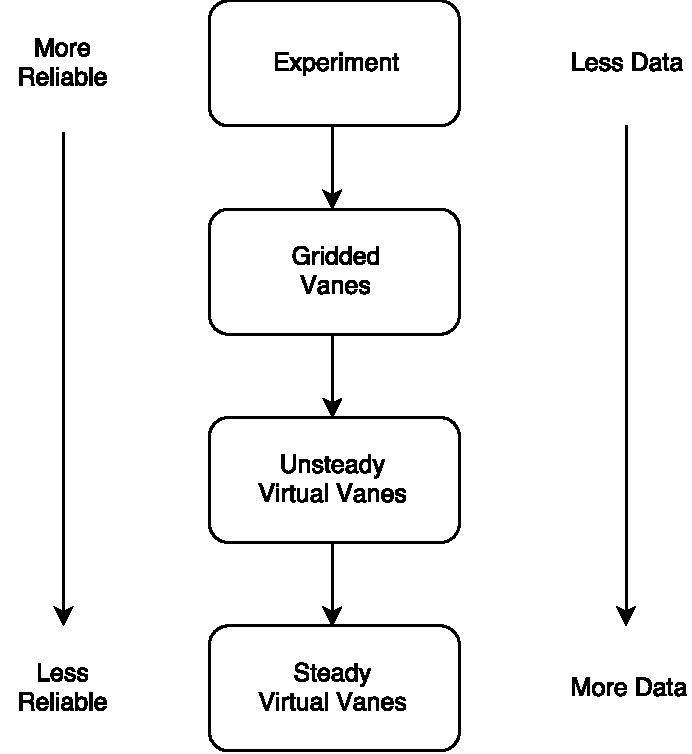
\includegraphics[width = 8 cm]{figs/validation_hierarchy}
    \caption{This figures depicts the validation hierarchy. The
    experimental measurements 
    are at the top, where the data is expected to be the most reliable,
    but simultaneously the most limited. Moving down the table leads to
    simulated data sources that are less reliable but increasingly
    cheaper in time to generate. At the bottom is the reduced order
    model from steady virtual vane solutions.} 
    \label{fig:val_hier}
   \end{center}
 \end{figure}

Three kinds of experimental validation data are available. These are
data generated in the laboratory using a heated plate, data from
experiments in the wind tunnel (``Wind-only''), and measurements from field
tests (``Field'') conducted in Arizona. The available data from
these cases and the gridded vanes created to mimic them are are
summarized in Table~\ref{tab:val_data}. Every case shown has been
simulated using the virtual vanes.   

%\large
\begin{table}[h]
\centering
\label{my-label}
\begin{tabular}{l|l|l|l|}
           & Wind-Only                   & Thermal-Only                & Field  \\
  \hline 
Experiment & Straight Vanes $60^{\circ}$ & Straight Vanes $60^{\circ}$ & June 2014   \\
           &                           & Straight Vanes $30^{\circ}$   & August 2014 \\
           &                           & Hybrid (Two tier)             & August 2015 \\
  \hline 
Gridded    & Straight Vanes $60^{\circ}$ & Straight Vanes $60^{\circ}$ & \\
           & Straight Vanes $30^{\circ}$ & Straight Vanes $30^{\circ}$ & \\
  \hline 
\end{tabular}
  \caption{Available truth data from the laboratory experiments 
    (cold wind and thermal-only), the field test, and the gridded vanes.} 
  \label{tab:val_data}
\end{table}
%
%
%
% http://www.tablesgenerator.com/
%
%


%
% experimental challenges
%
%\normalsize
\section{Thermal-Only Validation}
This section provides examples of the validation performed with the
richest data set, the measurements in the laboratory. All of the
thermal-only the data was generated in a laboratory setting at Georgia
Tech. The general system configuration is depicted in Figure
\ref{fig:lab_image}. These data were taken using stereo particle image
velocimetery (PIV) at Georgia Tech by Mark Simpson and Ari Glezer, and
the errors in in measurement and sampling are 
not quoted. The particles are seeded outside of the array vanes and
permitted to naturally convect into the turning vane enclosure. The
particles were from a glycol-water theatrical fog (Rosco Fog Fluid). 
Only velocity measurements are available. Several
potentially important quantities of interest, such as the pressure and
temperature, have not been measured.  

%
% http://convertonlinefree.com/ConvertImageEN.aspx
%
 \begin{figure}[!htb]
   \begin{center}
    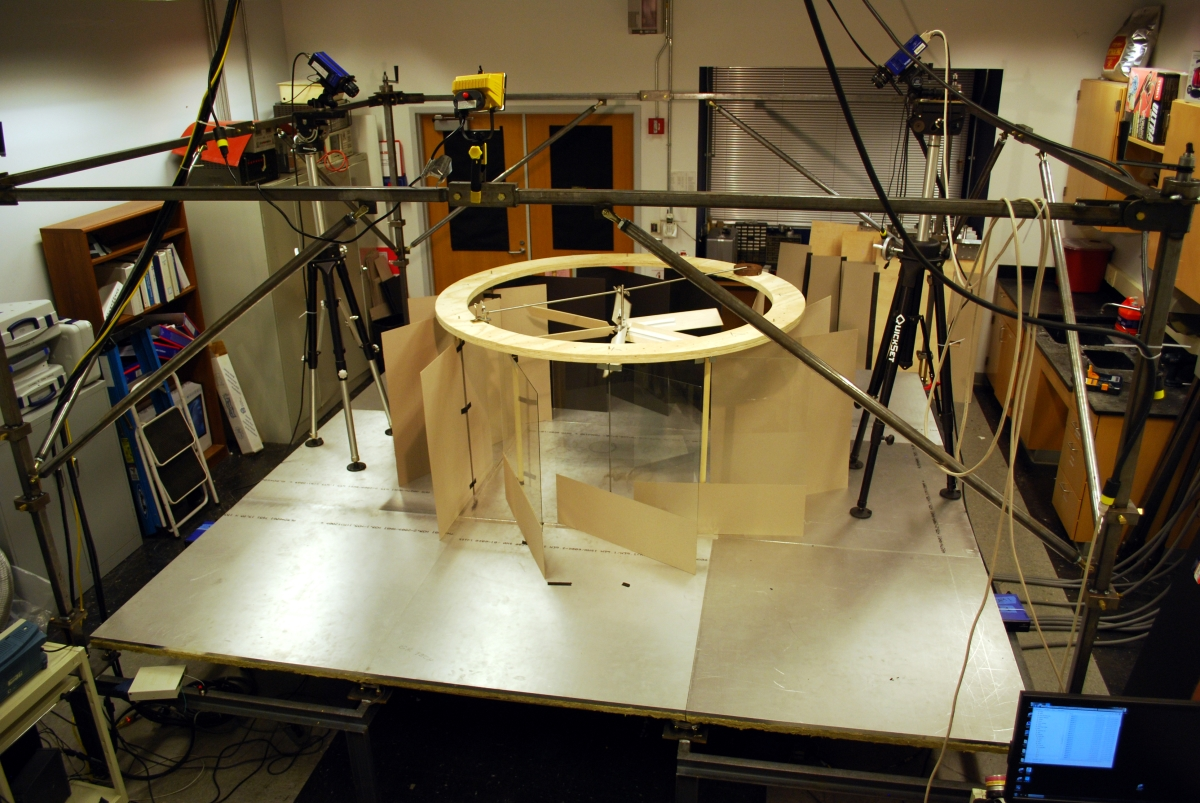
\includegraphics[width = 12 cm]{figs/Optimized-lab_setup}
    \caption{The single tier straight vane laboratory configuration. The
    apparatus is shown with a turbine, but that was removed for data
    gathering. The particles for PIV were seeded outside of the turning
    vanes and entrained into the central region.}
    \label{fig:lab_image}
   \end{center}
 \end{figure}

While no sensitivity analysis has been performed, it is likely that the
largest uncertainty in the laboratory simulation is a result of the
ventilation of the laboratory. The heated plate at the bottom of the apparatus
generates enough heat to cause a significant increase in room
temperature (30+ Kelvin), which greatly impacts the SoV
performance, as the ground to air thermal gradient drives the
vortex. The laboratory is cooled to maintain
temperature by two inlet HVAC ducts into the room. 
%While efforts have been made to characterize the level of ventilation being
%used, these numbers come with non-trivial uncertainties attached. 
One vent continuously provides air at 288 Kelvin with a flow rate estimated 
to be 1 $\text{m}^3$/s.
%(4-6 m/s with an approximate area of 0.2 $m^2$)
The other vent is active only if the room temperature exceeds 301 Kelvin, 
with a flow rate also estimated at 1 $\text{m}^3$/s.
Finally, the air leaves through the cracks around the laboratory doors and 
exhaust vents. Preliminary results indicated that an inflow rate of 1
$\text{m}^3$/s, the lower bound of the possible inflow rates results in
excessive heating of the room, while inflow conditions at the maximum
inflow rate of 2 $\text{m}^3$/s result in a simulated room that is too cold,
compared to the laboratory.  

Our simulated vortices are sensitive to ambient room temperature and thus 
the inflow rate. It is likely that the laboratory is run where one of
the vents is operating intermittently. 
To mimic these conditions in our simulations, Dirichlet boundary conditions 
on parts of the sides of the computational domain are used to
establish a constant inflow of cool air at the rates 
proscribed by our collaborators. Over the remainder of the side walls, 
adiabatic thermal boundary conditions are are used. 

The most signficant boundary condition disparity is that flow leaves the
domain through the top boundary, instead of out of the sides of the
room. Preliminary results suggested that the SoV phenomenon  was not
sensistive to these boundary condition details. The important element is
the  global energy balance in the room. The flow rate into the room is
adjusted to  1.3 $m^3$/s for the validation results discussed here.  

%% \begin{figure}[!htb]
%%   \begin{center}
%%    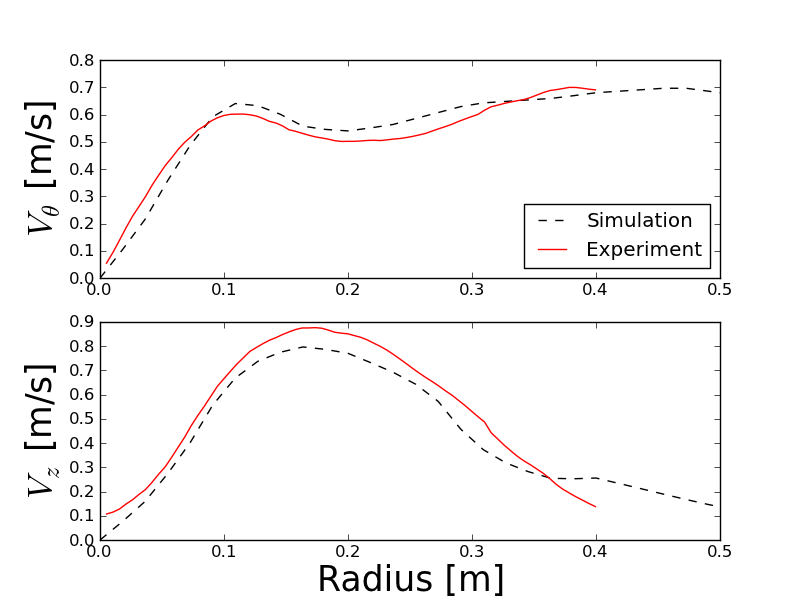
\includegraphics[width = 12 cm]{figs/hybrid_profile}
%%    \caption{Azimuthal and vertical velocity profiles as a function of
%%    radius. The simulation and experimental data broadly agree, with
%%    the simulation also exhibiting the characteristic ``twin-peak''
%%    structure of the hybrid vanes in the azimuthal velocity. }
%%    \label{fig:lab}
%%   \end{center}
%% \end{figure}

\todo{fix me}
% \begin{figure}[htp!]

%  \begin{subfigure}{.5\textwidth}
%   \centering
%   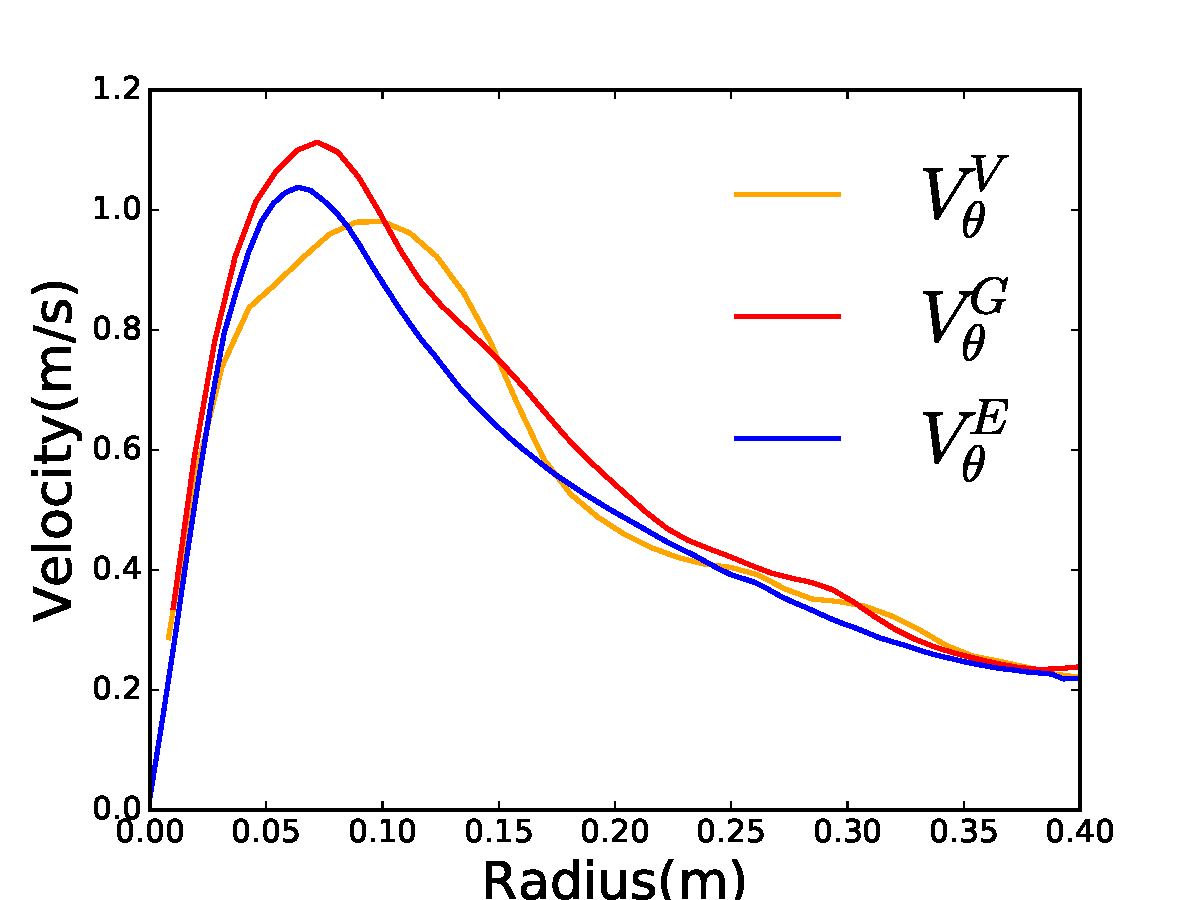
\includegraphics[width =0.9\textwidth]{figs/sim_vs_exp_30_vt}
%   \caption{Azimuthal velocity}
%  \end{subfigure}%
%  \begin{subfigure}{.5\textwidth}
%   \centering
%   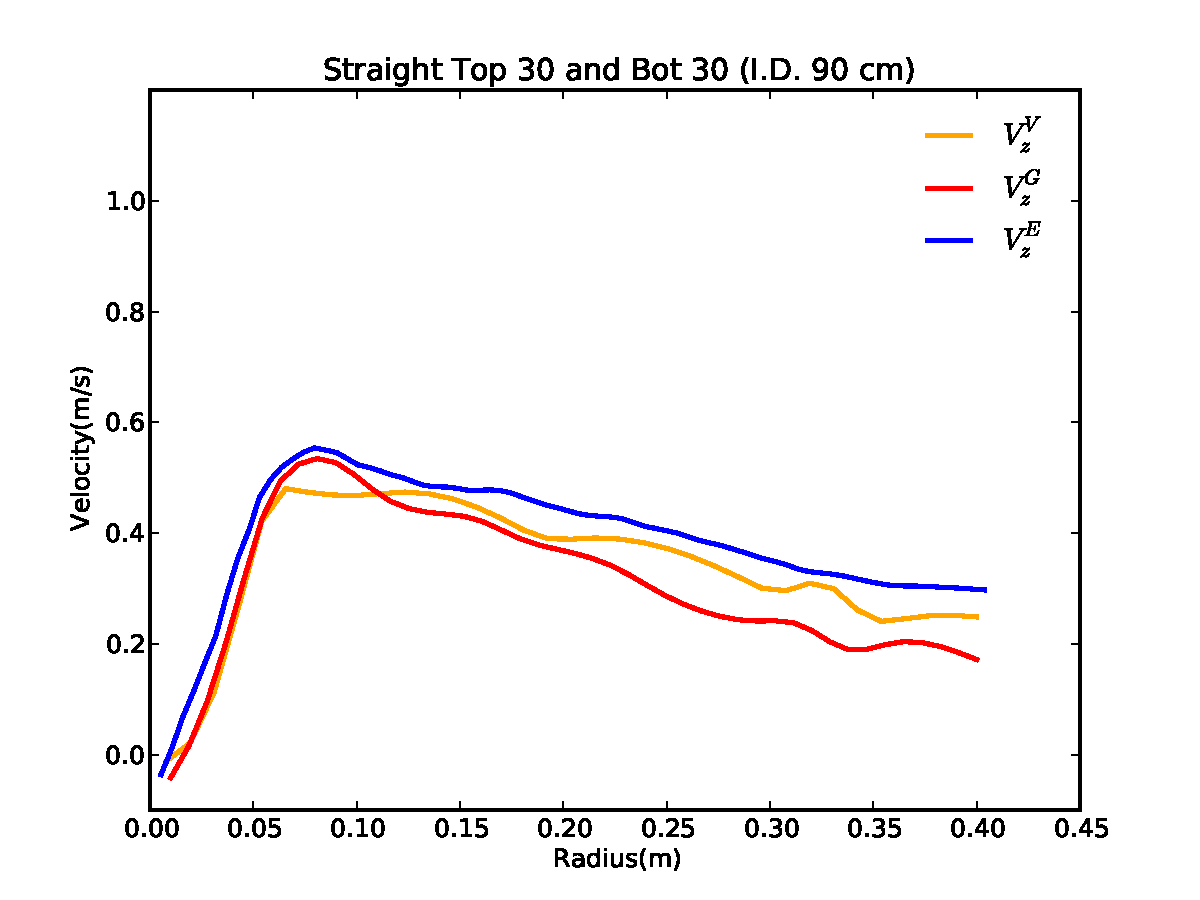
\includegraphics[width =0.9\textwidth]{figs/sim_vs_exp_30_vz}%
%   \caption{Vertical velocity} 
%  \end{subfigure}%
%   \caption{Azimuthal (left) and vertical (right) velocity 
%  as a function of radius for the thermal-only cases. The gold line is
%  the virtual vane simulation, blue the experiment, and red the gridded vane.} 
%   \label{fig:val_lab}  
% \end{figure}

Figure \ref{fig:val_lab} is a direct comparison between laboratory 
measurements for a simple single tier vane configuration ($30^{\circ}$
straight vanes) and nominally identical simulations with the gridded and
virtual vanes. The simulations and experiment broadly agree. The
simulation correctly reproduce the peak structure in the azimuthal
velocity observed for this configuration in the experiment. The gridded
vanes closely represent the peaks radial location, while the
virtual vanes over-predict the radial location. The radial location of
peak vertical velocity also closely agrees with experiment.

Similar validation comparisons have been made between several other
configurations with similar levels of agreement,  notably the
$60^{\circ}$ single tier straight vane case, and the two tier hybrid
vane.  Finally, estimates of the energy fluxes between the field
configuration and our simulation results agreed within 15\%. These
validation studies have provided a level of confidence that our
simulations accurately reproduce the phenomena observed in laboratory.

\section{Wind Cases}

The laboratory thermal vortex experiments described in the previous
section did not include the effects of the wind, but experience in
the field indicated how important these effects were. To ensure that the
virtual vanes could represent this effect, a validation study 
was performed using the data obtained in the wind tunnel.

A numerical experiment was performed in which the 60 degree single tier
straight vanes were placed in a isothermal wind.  These results were
compared to an identical configuration placed in a wind tunnel.
However, no measurements (of velocity or any quantity) were made
for the vanes in these conditions. Qualitative comparisons, based on
descriptions of observed structures and videos of smoke visualization
were made between the simulations and the wind tunnel experiments. These
images and discussions did not 
identify any inconsistencies between simulation and experiment.
However, these results are limited, and are only for the cold wind, as
the wind tunnel did not include a heated plate.  

\begin{figure}
  \centering
  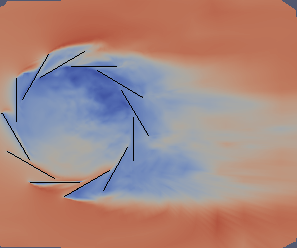
\includegraphics[width=.45\linewidth]{figs/gridded_wind}
  %\caption{Streamwise Velocity: Gridded Vanes}
  \hfill
  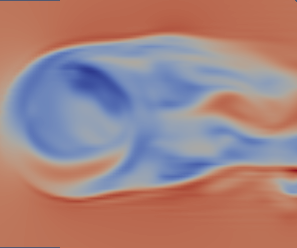
\includegraphics[width=.45\linewidth]{figs/virtual_wind}
  %\caption{Streamwise Velocity: Virtual Vanes}
  \\
  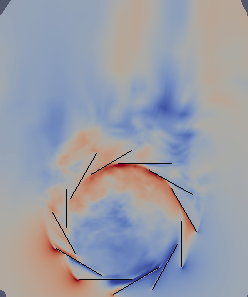
\includegraphics[width=.45\linewidth]{figs/gridded_wind_span}
  %\caption{Spanwise Velocity: Gridded Vanes}
  \hfill
  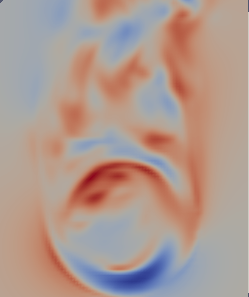
\includegraphics[width=.45\linewidth]{figs/virtual_wind_span}
 %\caption{Spanwise Velocity: Virtual Vanes}
  \label{fig:wind_val}
 \caption{Horizontal slices through the top of the vanes for the
 wind validation cases. On the left are the explicitly gridded vanes,
 and on the right the virtual vanes. The streamwise velocity shows
 penetration through the region where the vanes are aligned with the
 flow in both the gridded and virtual vanes. In addition, the
 virtual vane case correctly reproduces the direction and magnitude of
 the spanwise velocity inside the vanes. Finally, the wake has similar
 structure between the two cases.}

\end{figure}


\section{steady vs unsteady}
Talk about dialing in the viscosity for steady. Might have some good
plots I can pull out too\todo{write me}

Figure~\ref{fig:wind_val} contains images of the simulated averaged
streamwise and  spanwise velocity in a horizontal plane at approximately
the height of the vanes obtained from simulations with gridded and
virtual vanes. As expected, there are some differences in the
details of these simulations, but the overall character of the flow
inside the vanes, and in the wake of the vanes is quite similar. This
demonstrates that the virtual vane formulation can indeed represent the
interaction with the wind. 

\section{Field Configurations}

Several field tests have been performed by the experimental team. After
each field test, qualitative observations, measurements and lessons
learned are provided by the field team. Actual measurements
are limited. Due to the complexity of the configuration
(two vane tiers and a cone) Gridded vanes cases have not been developed
for the field. This section provides a discussion of some of
the results from the latest field test, as an example of typical
validations performed. 

 \begin{figure}[!htb]
  \begin{center}
   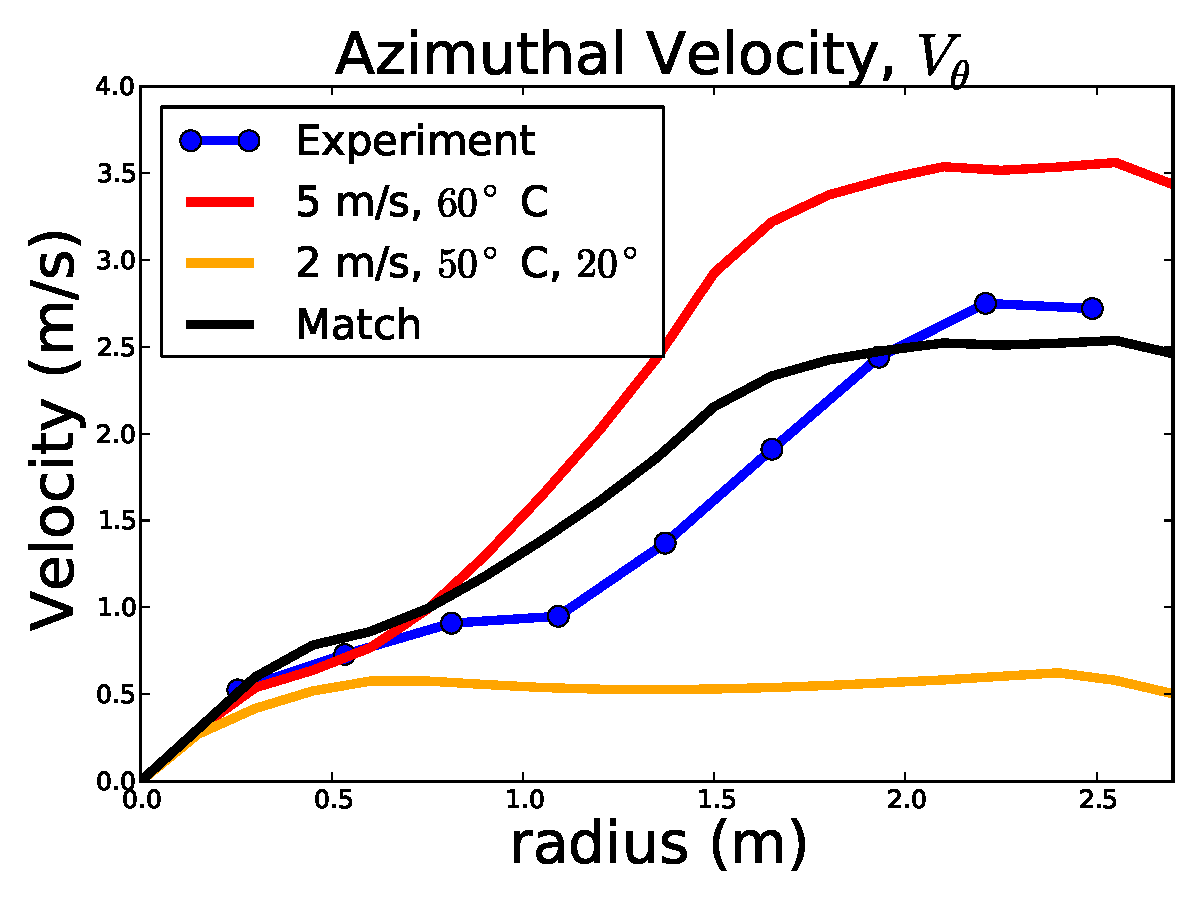
\includegraphics[width = 12 cm]{figs/validate_field}
   \caption{Azimuthal velocity data from the August 2015 field test is
   shown in blue. Two virtual vane simulations with different scenario
   parameters are shown in red and gold. The velocity field was
   temporally averaged but not averaged in space, to reproduce
   the measurements from the field.}
   \label{fig:field_val}
  \end{center}
 \end{figure}
%
% provide an example of these validations below
%

Figure~\ref{fig:field_val} shows data from the August 2015 field test in
blue. These results were obtained using an anonmometer at fixed
azimithal location (believed to be a ninety degree angle, where the zero
is defined to be aligned with the streamwise flow direction) to measure the
azimuthal velocity. The ultrasonic 
anemometer malfunctioned, and the temperature was only measuered at one
location at 1 meter height. A time series from approximately an hour was
gathered. This data included large scenario uncertainties, with
estimated 3 m/s variations in wind, 20 degree wind heading changes, and
10 degree Celsius shifts in temperature. A solidworks CAD file provided
by the experimental team defined the vane and cone
geometry, which were then represented in the simulations as virtual
vanes and a solid surface, as described in 
Chapters~\ref{subsec:vane} and~\ref{subsec:solid_surface}.   

To span the range of conditions, several simulations were conducted
with different scenario parameters. The azimuthal velocity from two such
simulations (Red and Gold lines) are plotted against the experimental
data (blue line) in Figure~\ref{fig:field_val}.  

These simulations accurately bound the experimental data. Furthermore, a
``Matching'' case was identified that is broadly consistent with the
field results. The kinetic energy flux, measured in a horizontal plane
at the top of the vanes (where a turbine to extract this energy would
likely be placed), in the simulations agrees with the experimental
estimate within 10\%. 


%
% validation story is incomplete
% 
% you have done: 
%
% 1) comparions between laboratory + gridded + virtual 
% 
% 2) comparisons between gridded + virtual in laboratory
%    + field configurations, thermal only and wind
%
% 3) comparisons of virtual vanes to field observations 
%    quantitative + qualitative
%
%
% You need to discuss what needs to be validated -- the
% comparison to gridded vanes is a useful validation tool 
%


\chapter{Characteristics of Synthetic Dust-Devils}
\label{sec:results}

%
% RESULTS TODO
%
% need to motivate optimization workflow and plans
% current ideas not bad, need more
%
%

This chapter details some of the early simulations and investigations
of the SoV. The chapter begins with a study of the thermal-only
conditions, and the optimization of the vanes in this scenario. It then
proceeds to a simple wind case. Next, a discussion of the optimization
procedure is detailed. Finally, the chapter attempts to discern some of
the physical processes driving the SoV. The effect of the wind versus
the thermally-drive buoyancy is investigated. The chapter concludes with
comparisons between the synthetic dust-devils of the SoV and available
data from the natural variety. 

\section{Thermal Only}
\label{sec:thermal_only}

While ambient winds in the field impact system performance, it is
also illuminating to consider an idealized scenario with natural
convection driven only by thermal instabilities. Simulations of this
baseline, thermal-only flow are intended to ensure the SoV apparatus to
form a strong thermal plume even in the absence of
wind. Programmatically, these simulations were conducted before the
introduction of the wind, as the fully extent of the wind's impact was
not yet realized. 

In this section a representative case of an optimized thermal-only SoV
configuration is presented. This is a simple curved vane configuration with
two-tiers with ground temperature of 335 Kelvin and a freestream
temperature of 313 Kelvin. There is no ambient velocity and the boundary
conditions are as described in Chapter~\ref{sec:bc}.  

The two tiers of vanes used for these cases are drawn in~\todo{add table}
Figures~\ref{fig:thermal_vane_bottom} and \ref{fig:thermal_vane_top}.  
Note that in the configuration, the vanes are aligned radially at the
largest radius, and then increasingly curve towards azimuthal at smaller
radius. Note that these are representative curves of the body forcing
field, and do not actually represent vane surfaces. The vanes are
represented as in Chapter~\ref{subsec:vane}.  These images are created
by tracing the path a particle follows through the forcing field. The
region of forcing is between $\{0.3-0.9\}$ meters for the bottom tier,
and $\{0.6-0.9\}$ meters for the top tier. Overall, the system is 1.1
meters tall, with the short first tier only standing 0.132 meters
high. The top and bottom tiers have final angles of $70^{\circ}$ and
$85^{\circ}$, respectively. No cone is used in this case. 

\begin{figure}[htb]
\centering
\begin{minipage}{0.45\textwidth}
\centering
 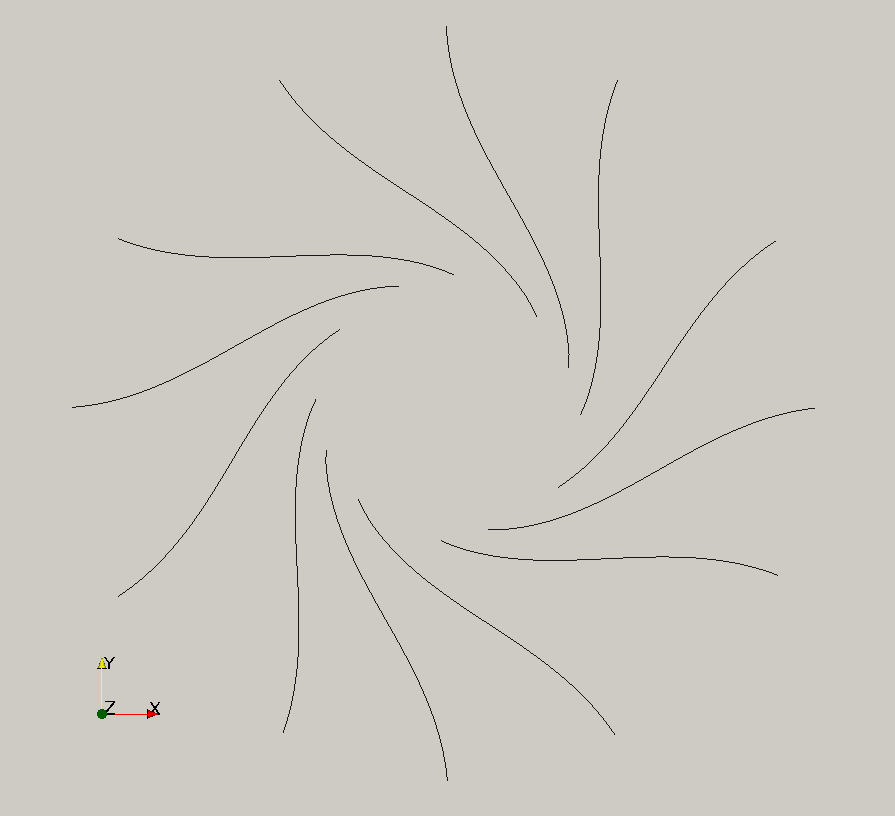
\includegraphics[width=.8\linewidth]{figs/bottom_thermal_only}
 \caption{Horizontal drawings of the curvature functions for the bottom tier
 vanes. The max angle is $85^{\circ}$, or $5^{\circ}$ less than azimuthal.}
 \label{fig:thermal_vane_bottom}  
\end{minipage}\hfill
\begin{minipage}{0.45\textwidth}
\centering
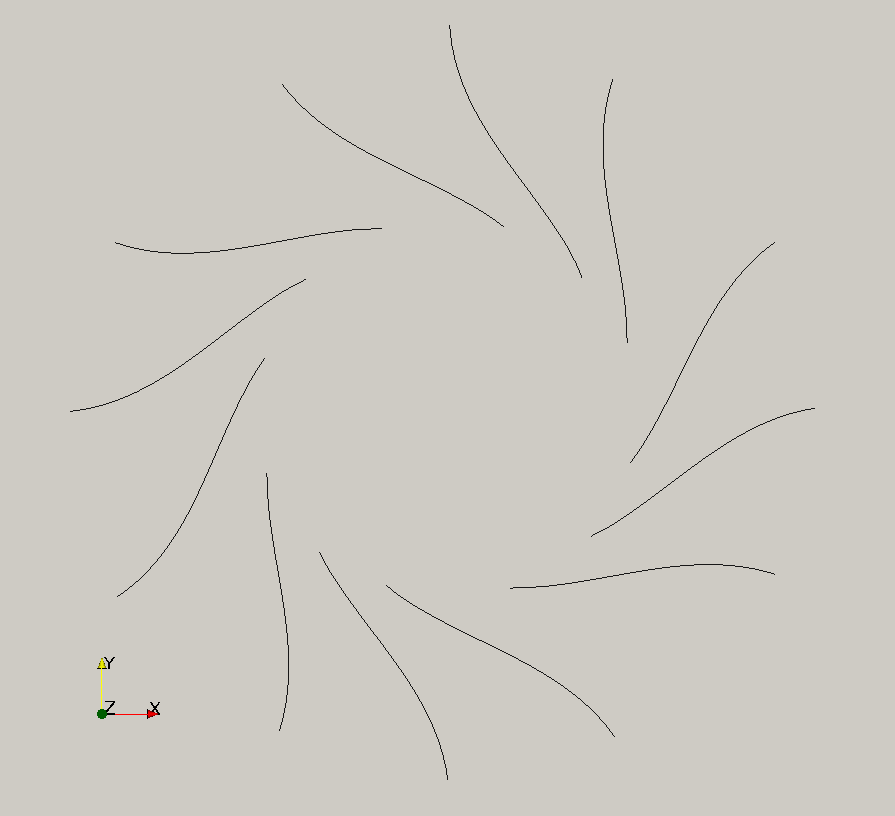
\includegraphics[width =0.8\textwidth]{figs/top_thermal_only}
\caption{Horizontal drawings of the curvature functions for the top tier
 vanes. The max angle is $70^{\circ}$, or $20^{\circ}$ less than
 azimuthal.} 
 \label{fig:thermal_vane_top}  
\end{minipage}
\end{figure}

\begin{figure}[htb]
\centering
\begin{minipage}{0.45\textwidth}
\centering
 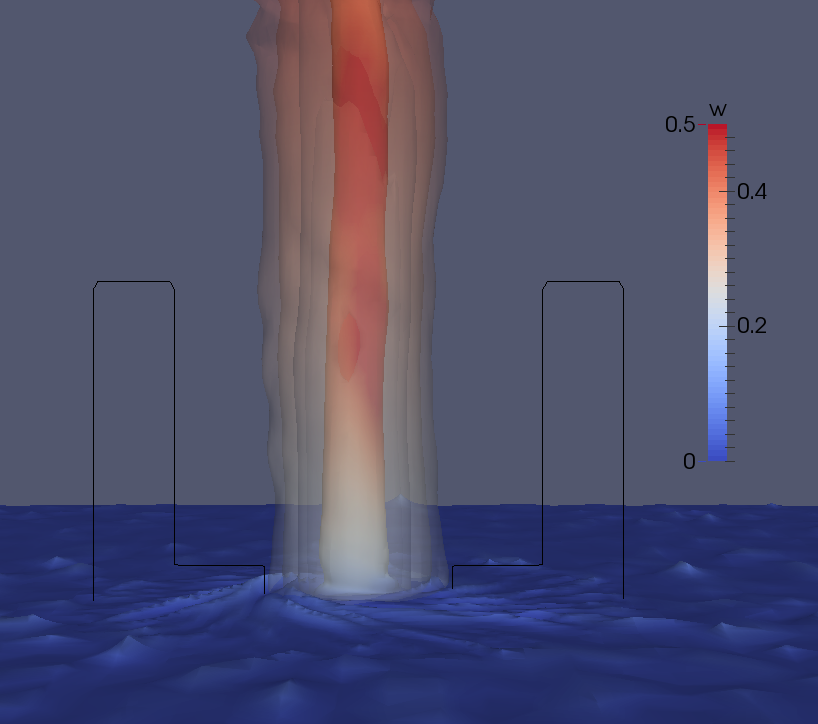
\includegraphics[width=.8\linewidth]{figs/3d}
 \caption{Isocountours of the inner thermal core
  visible through semi-transparent contour around azimuthal velocity,
  colored by vertical velocity. This shows that the thermal core creates
 an upward flow, which entrains and rotations fluid around it. An
 outline of the region of virtual vanes has been drawn.}
 \label{fig:thermal}  
\end{minipage}\hfill
\begin{minipage}{0.45\textwidth}
\centering
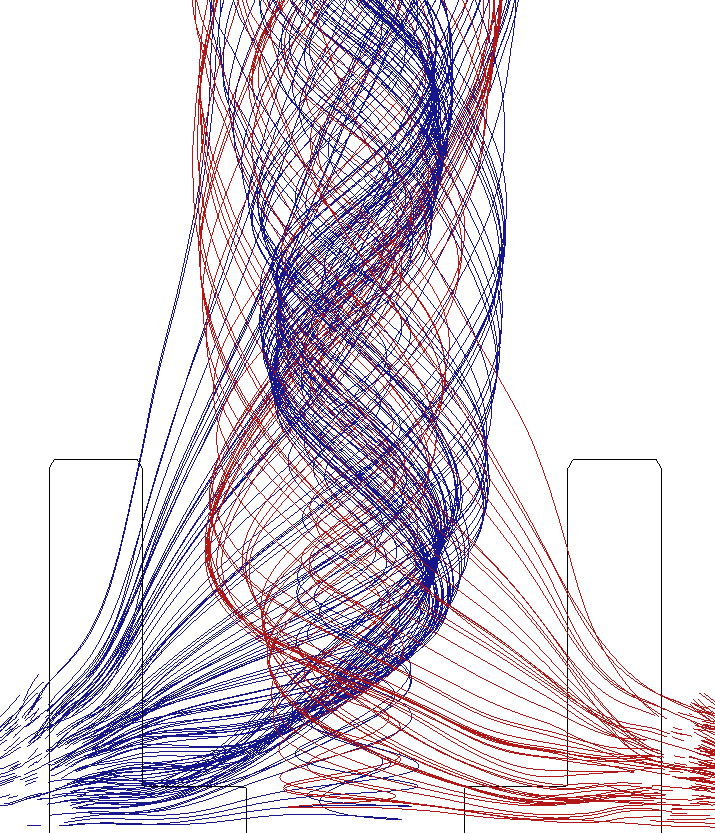
\includegraphics[width =0.8\textwidth]{figs/entrainment}
\caption{Fluid entrainment around the apparatus. This was drawn by
 seeding particles into the averaged flowfield and then advancing them
 using an RK4 time integrator. An outline of the
  virtual vanes are drawn to show the region of forcing.}
 \label{fig:entrain}  
\end{minipage}
\end{figure}


% \begin{figure}[htb]

%  \begin{subfigure}{.55\textwidth}
%   \centering
%   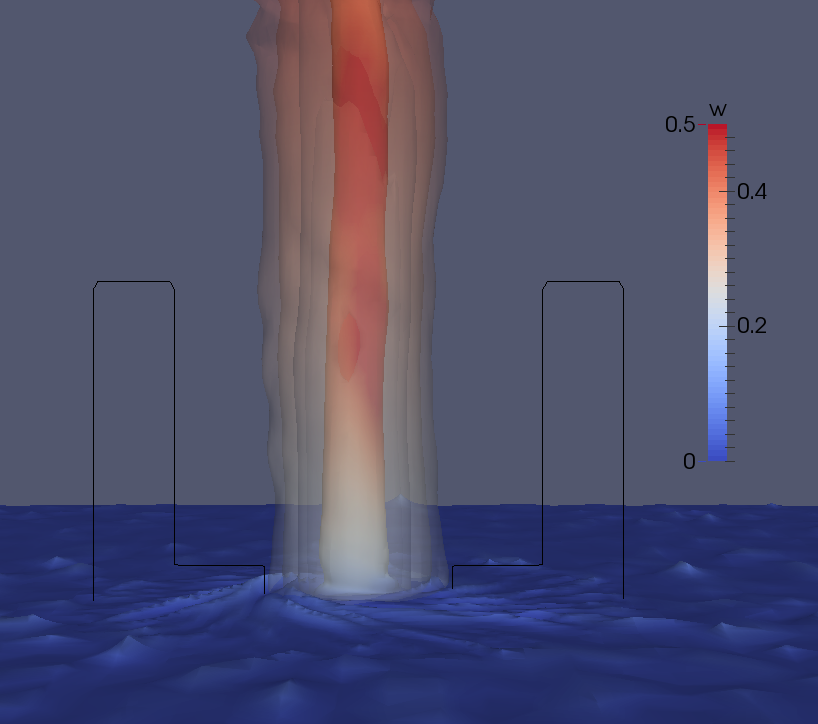
\includegraphics[width =0.7\textwidth]{figs/3d}
%   \caption{Isocountours of the inner thermal core
%   visible through semi-transparent contour around azimuthal velocity,
%   colored by vertical velocity. An outline of the region of virtual
%   vanes has been drawn.}
%   \label{fig:thermal}  
%  \end{subfigure}%
%  \begin{subfigure}{.4\textwidth}
%   \centering
%   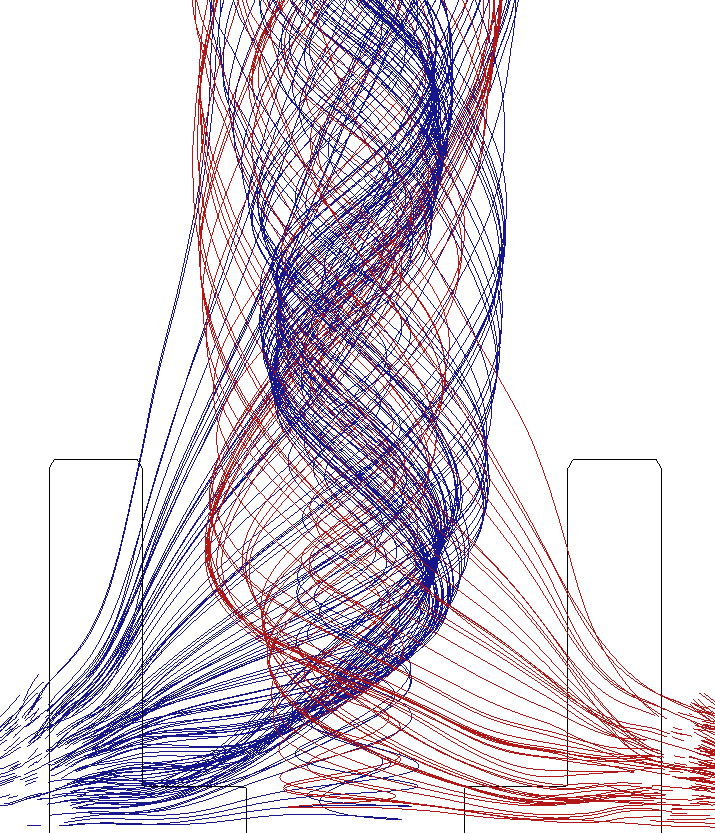
\includegraphics[width =0.8\textwidth]{figs/entrainment}%
%   \caption{Fluid entrainment around the apparatus. An outline of the
%   virtual vanes are drawn to show the region of forcing.} 
%   \label{fig:entrain}  
%  \end{subfigure}%
% \end{figure}

The results shown were from transient solutions (the unsteady virtual
vanes) and so the images of the fields are averages of fifty snapshots
of the solution taken over the course of ten minutes. In general, the
averaging times are selected to be approximately 20 to 30 wash-out
times, where a wash-out is defined as the time required for a particle
at the base of the apparatus to flow out through the top boundary. The
kinetic energy flux through the top of the vanes for this case is about
53 watts. The solution demonstrates several features characteristic of
naturally occurring dust devils. Figure~\ref{fig:thermal} shows a
temperature isocontour set at threshold of 3 Celsius higher than the
ambient fluid temperature. This value was selected because it was noted
by Sinclair~\cite{Sinclair1969} as characteristic of the thermal core 
temperature above the ambient temperature observed in dust devils. The
image depicts a tight, coherent thermal plume roughly the same size as
the inner diameter of the lower vanes. As anticipated, this hot flow is
acting like a chimney, generating a large vertical velocity which in
turn entrains air from the outside.  

An image of the entrainment is shown in Figure~\ref{fig:entrain}. The
image was created by tracking particles as they convect through the
device. Tracer particles were seeded into the averaged flowfield and
then advancing through  the field using an RK4 time integrator.  
\todo{define how this is actually performed, mathematically}
There is clearly a tight inner vortex with significant azimuthal
velocity and a broader region of entraining fluid through the upper tier
of vanes.    

\begin{figure}[htb]

 \centering
 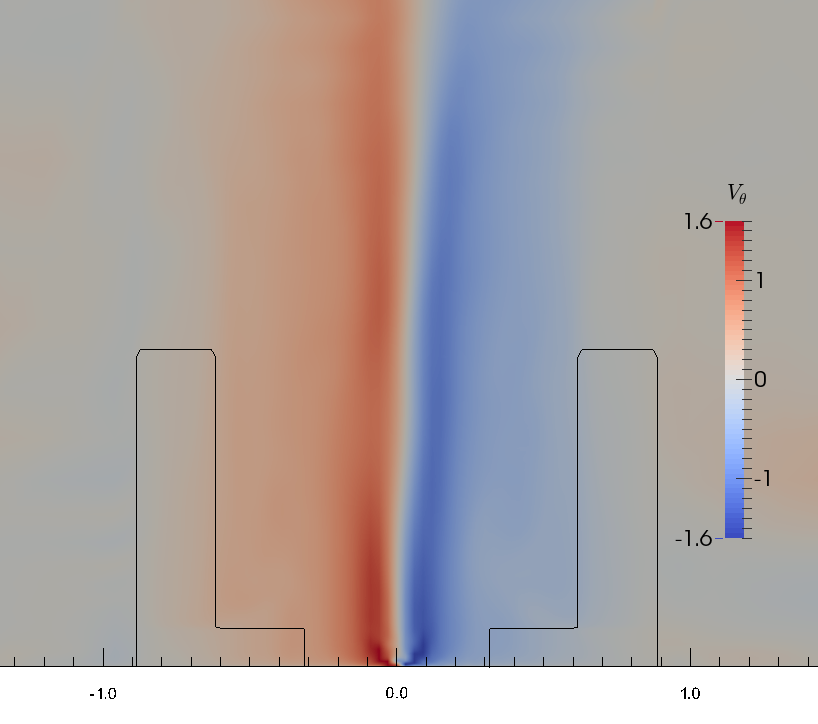
\includegraphics[width=.45\linewidth]{figs/vt}
 % \caption{Azimuthal Velocity}
 % \label{fig:vt-to}
 \hfill
  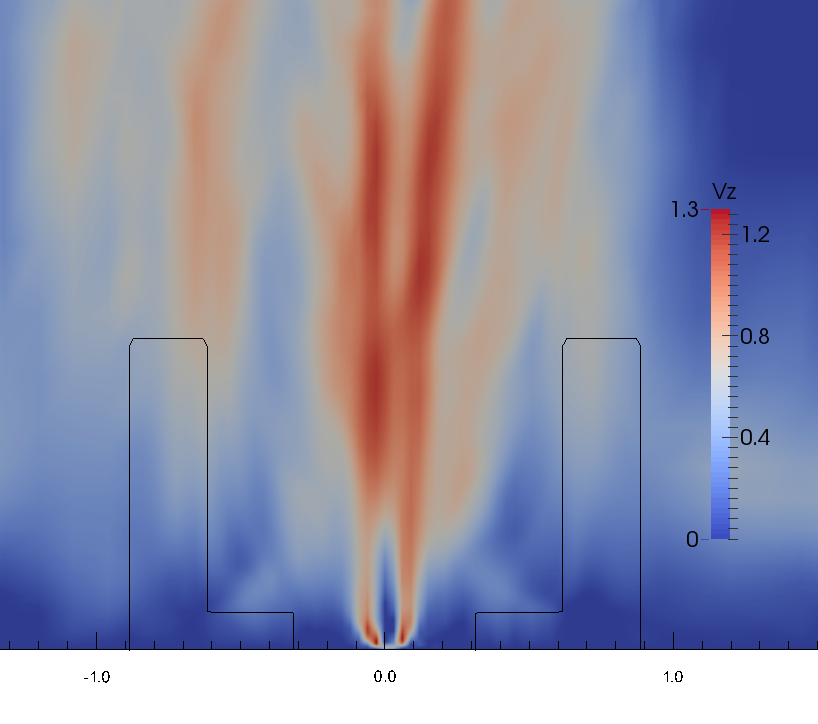
\includegraphics[width=.45\linewidth]{figs/vz}
 %\caption{Vertical Velocity}
 % \label{fig:vz-to}
 \\
  \centering
  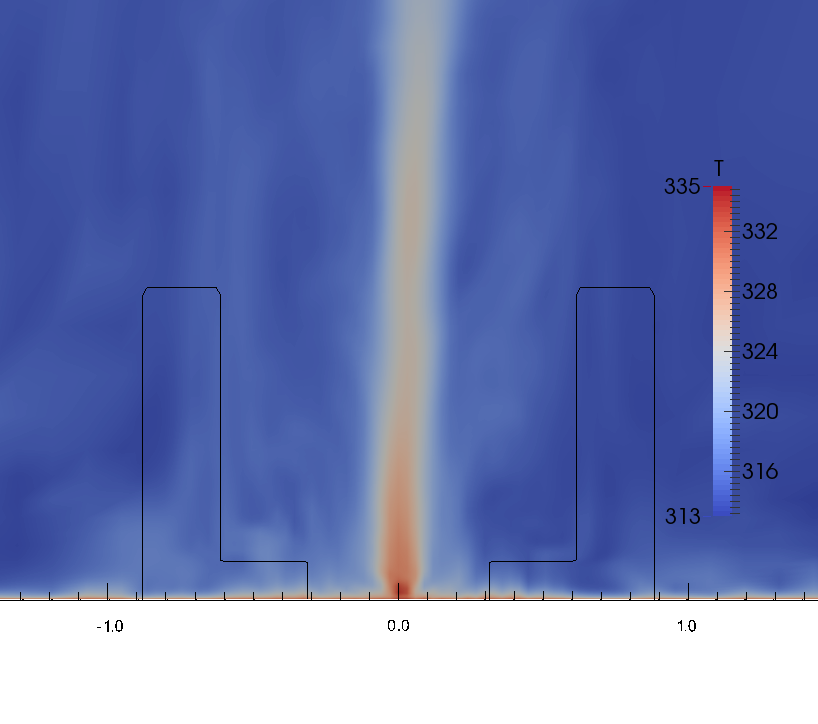
\includegraphics[width=.45\linewidth]{figs/t}
 %\caption{Temperature}
 % \label{fig:t-to}
 \hfill
 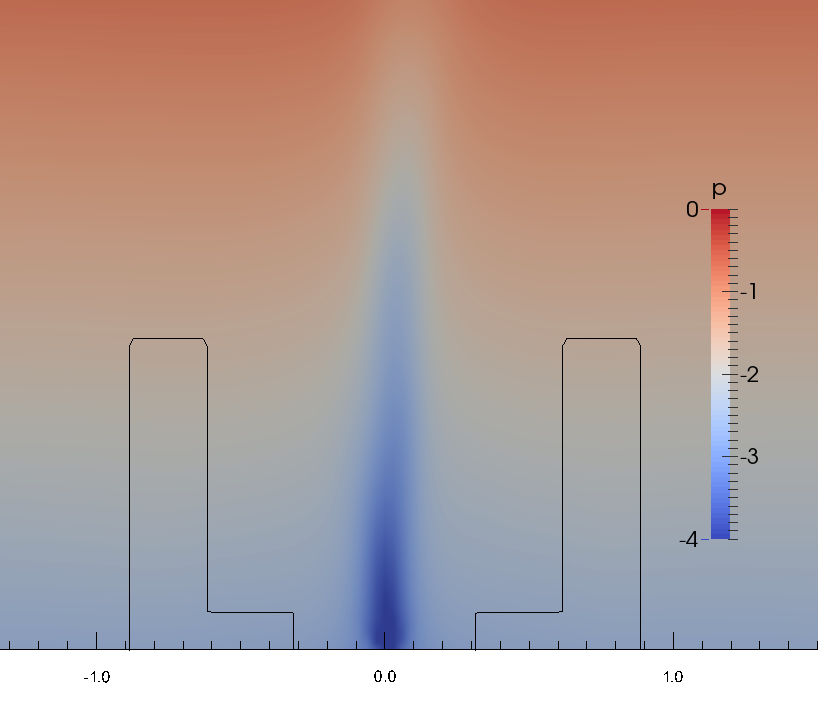
\includegraphics[width=.45\linewidth]{figs/p}
 % \caption{Pressure}
 % \label{fig:p-to}
 \caption{Time averaged vertical slices through the center of the device
 for the thermal-only cases. Black lines indicate the location of the
 vanes. A strong thermal plume is visible at the center of the device,
 which drives a vertical velocity. The fluid flow is entrained by this
 vertical movement and pulled radially into the center while being
 turned by the turning vanes. Notice also the low pressure ``eye'' at
 the center of the flow, and the modest downward flow in the  center of
 the vertical velocity, consistent with Figure~\ref{fig:cartoon}.} 
 \label{fig:to-vert}
\end{figure}

%
%
%
Figure~\ref{fig:to-vert} depicts several vertical slices through the SoV
for various state variables. One can see that there is a tight core
vortex with azimuthal and vertical velocities of several meters per
second. The tight vortex region coincides with a high temperature, low
pressure core region. The rapidly rotating air near the center induces
a low pressure core, as observed in real dust devils.
On the vertical velocity plot, a small downward flow region has formed in
the middle of the vortex, consistent with the sketch in
Figure~\ref{fig:cartoon}.   

\begin{figure}[htb]

 \centering
  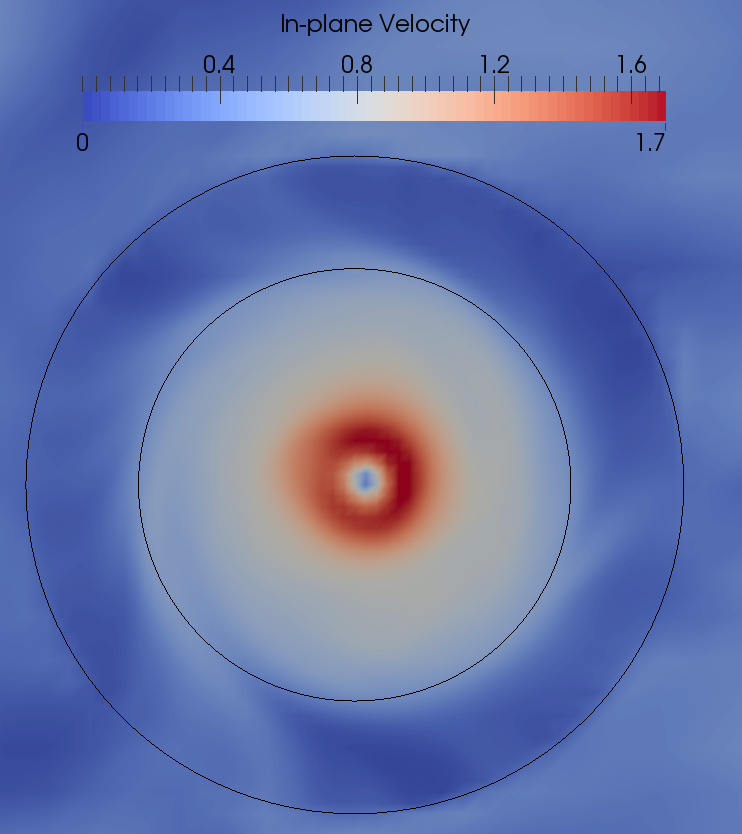
\includegraphics[width=.32\linewidth]{figs/vt_hor}
 %\caption{Azimuthal Velocity}
 % \label{fig:vt-to}
 \hfill
  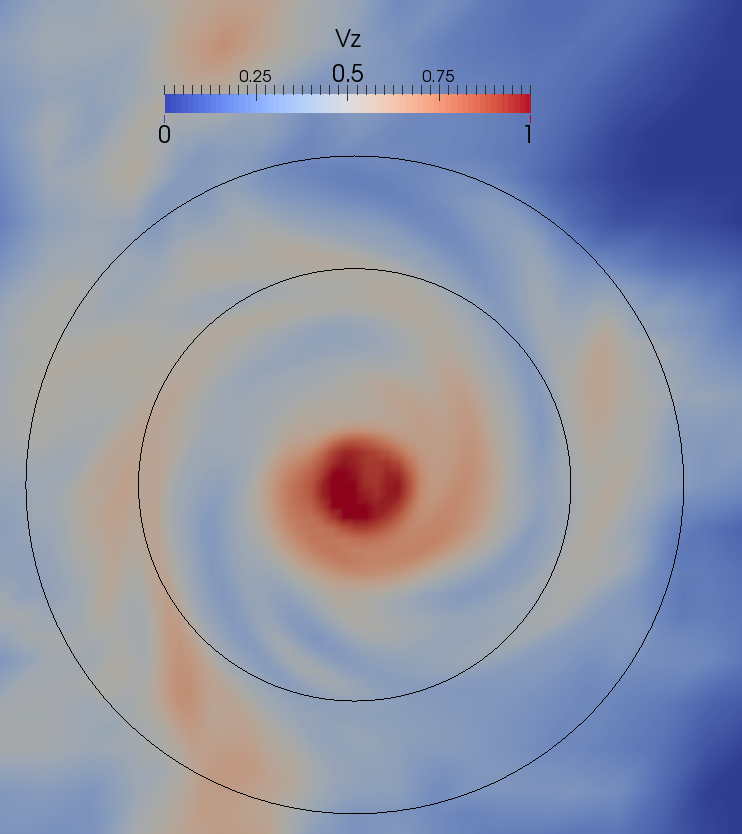
\includegraphics[width=.32\linewidth]{figs/vz_hor}
 % \caption{Vertical Velocity}
 % \label{fig:vz-to}
 \hfill
  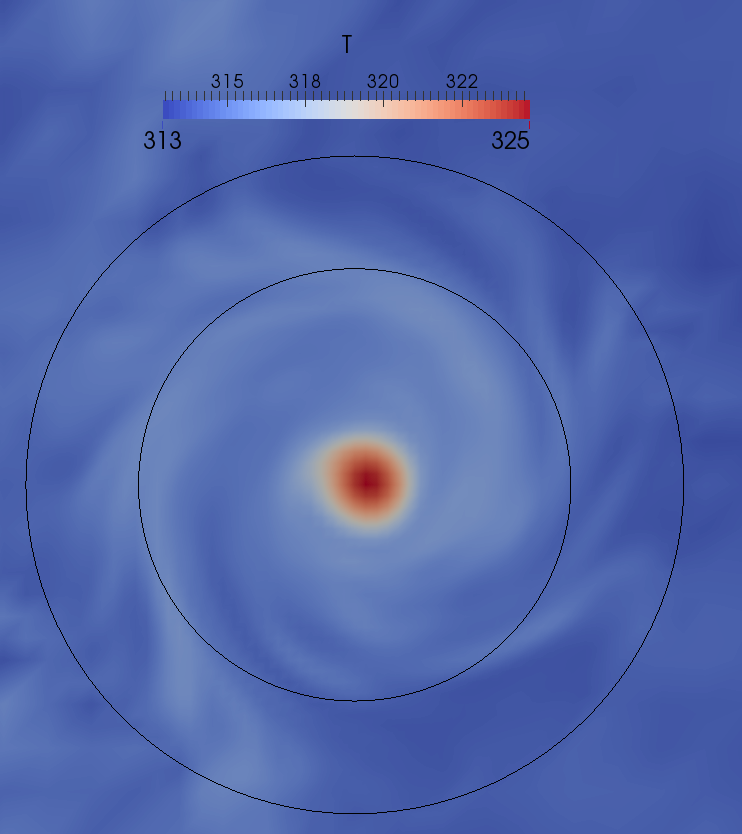
\includegraphics[width=.32\linewidth]{figs/t_hor}
 % \caption{Temperature}
 % \label{fig:t-to}
 \caption{Time averaged horizontal slices taken at the height of the
 second tier of vanes for the thermal-only cases. These images show a
 clear thermal plume driving a strong vertical velocity. Notice also the
 low downward velocity ``eye of the storm'' in (a). In contrast to the
 wind cases, the vortex is well-anchored in the center of the apparatus. }
 \label{fig:to-hor}
\end{figure}

Figure~\ref{fig:to-hor}, depicts several horizontal slices
through the SoV for the same state variables. It can be seen that the
large velocities are highly localized to a region just inside the
vanes. Likewise, the entrainment of fluid is limited to a region
immediately surrounding the vanes.\todo{fix axes to make readable} 
%
% conclusion of thermal only
%
Finally, the thermal plume is relatively narrow compared to the diameter
of the device. It is desirable to broaden the thermal plume, as this
would create a larger vertical momentum flux and consequentally a larger
kinetic energy flux.  

The diameter of the thermal core is therefore a critical flow
characteristic in the thermal-only conditions. However, a means of
setting the thermal plume's thickness is not presently 
known. Regardless, these slices lend credibilty to the 
notion that our turning vane configuration is generating something with
visible parallels to a naturally occurring dust devil.   

\section{Wind}

The wind case is for a 5 m/s ambient wind with a ground temperature of
335 Kelvin and freestream temperature of 313 Kelvin. There is no ambient
velocity and the boundary conditions are as described in
Chapter~\ref{sec:bc}. The vanes are drawn in
Figures~\ref{fig:wind_bottom} and \ref{fig:wind_top}. These images show
the straight vane case, and a cone that sits on top of the second tier of vanes. 
As in the previous section, these images are representative
curves of the body forcing field, and do not actually represent vane
surfaces. The vanes are represented as in Chapter~\ref{subsec:vane}. 
These images are created by tracing the path a particle follows through
the forcing field. The region of forcing is between $\{0.96-3.4\}$ meters
for the bottom tier, and $\{1.5-3.4\}$ meters for the top tier. Overall,
the system is three meters tall, with the short first tier only standing
0.3 meters high. The top and bottom tiers have final angles of
$70^{\circ}$ and $80^{\circ}$, respectively.\todo{add newer and fixed up
wind images}

\begin{figure}[htb]
\centering
\begin{minipage}{0.45\textwidth}
\centering
 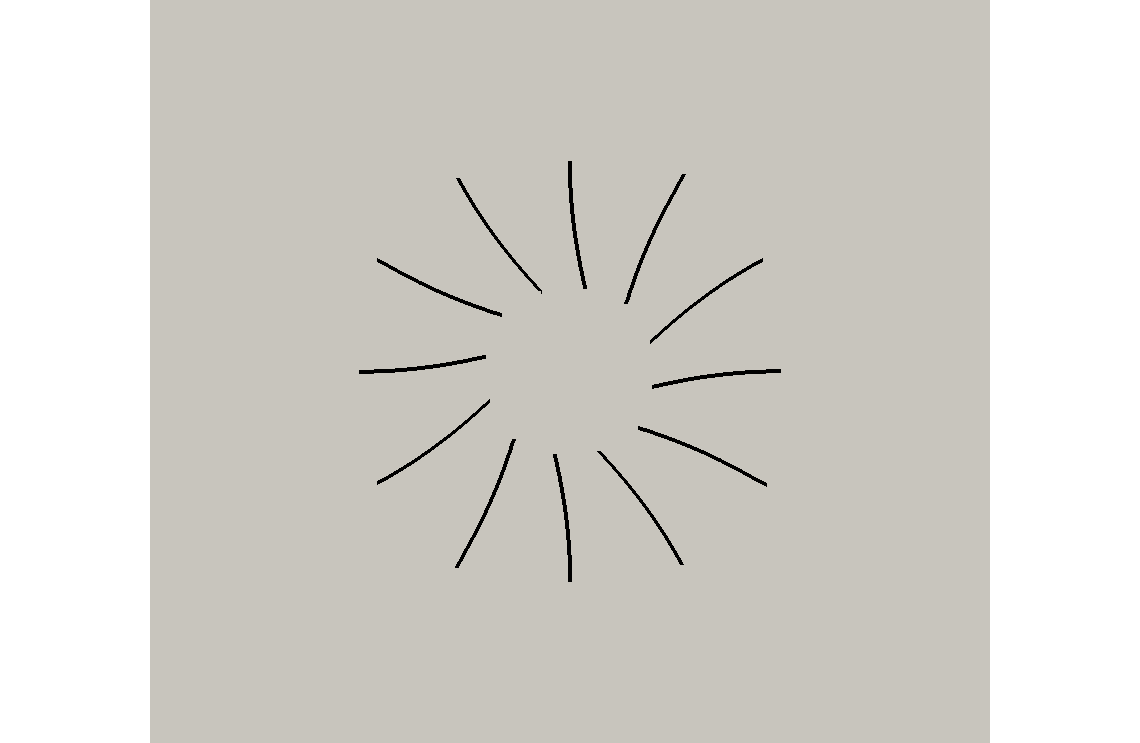
\includegraphics[width=.8\linewidth]{figs/wind_bottom}
 \caption{Horizontal drawings of the bottom tier vanes. These are curved 
 vanes with a final angle of $80^{\circ}$.}
 \label{fig:wind_bottom}  
\end{minipage}\hfill
\begin{minipage}{0.45\textwidth}
\centering
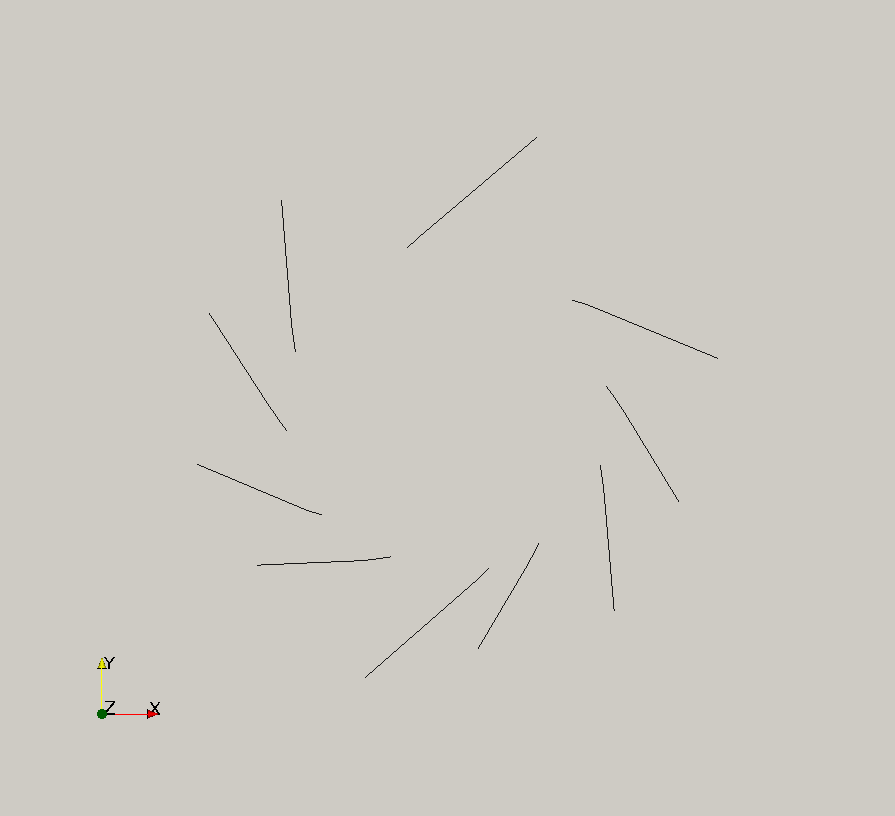
\includegraphics[width =0.8\textwidth]{figs/wind_top}
\caption{Horizontal drawings of the top tier vanes. These are straight
 angle vanes set at $70^{\circ}$.} 
 \label{fig:wind_top}  
\end{minipage}
\end{figure}


%
% horizontal slices
%
\begin{figure}[htb]

  \centering
  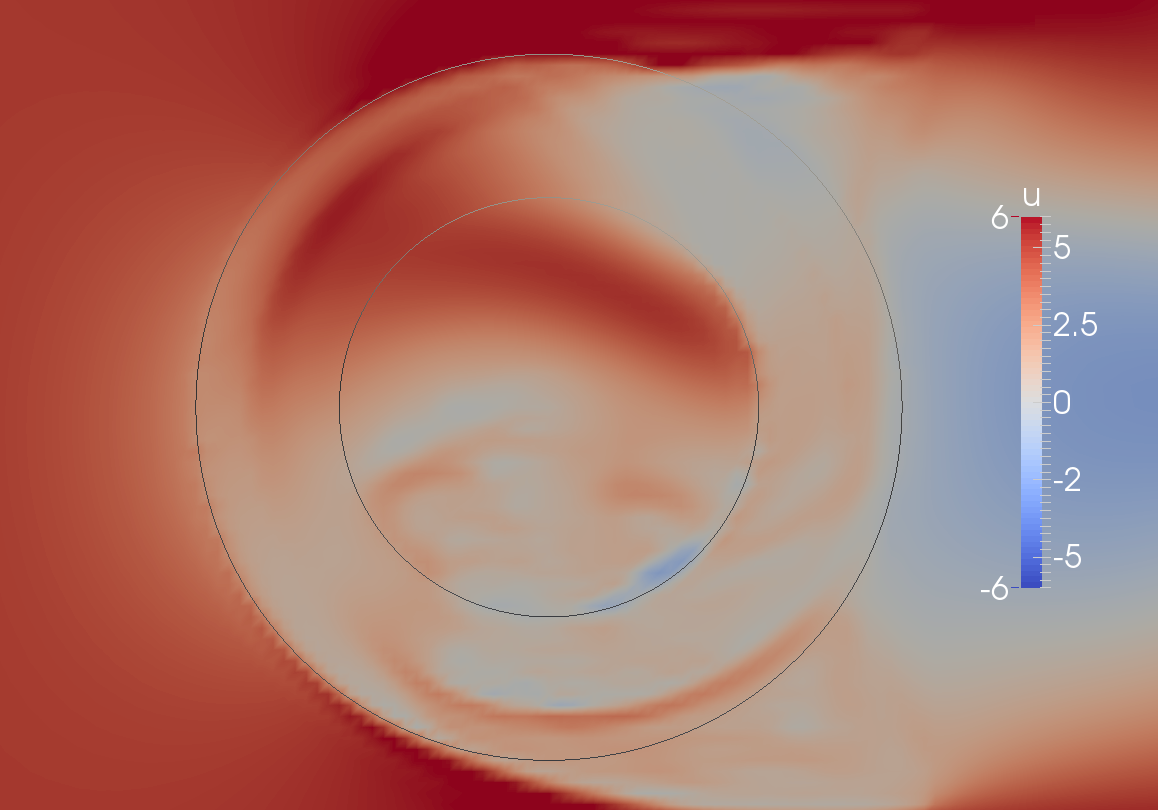
\includegraphics[width=.47\linewidth]{figs/wind_u}
 %\caption{Streamwise}
 % \label{fig:vt-wind}
 \hfill
  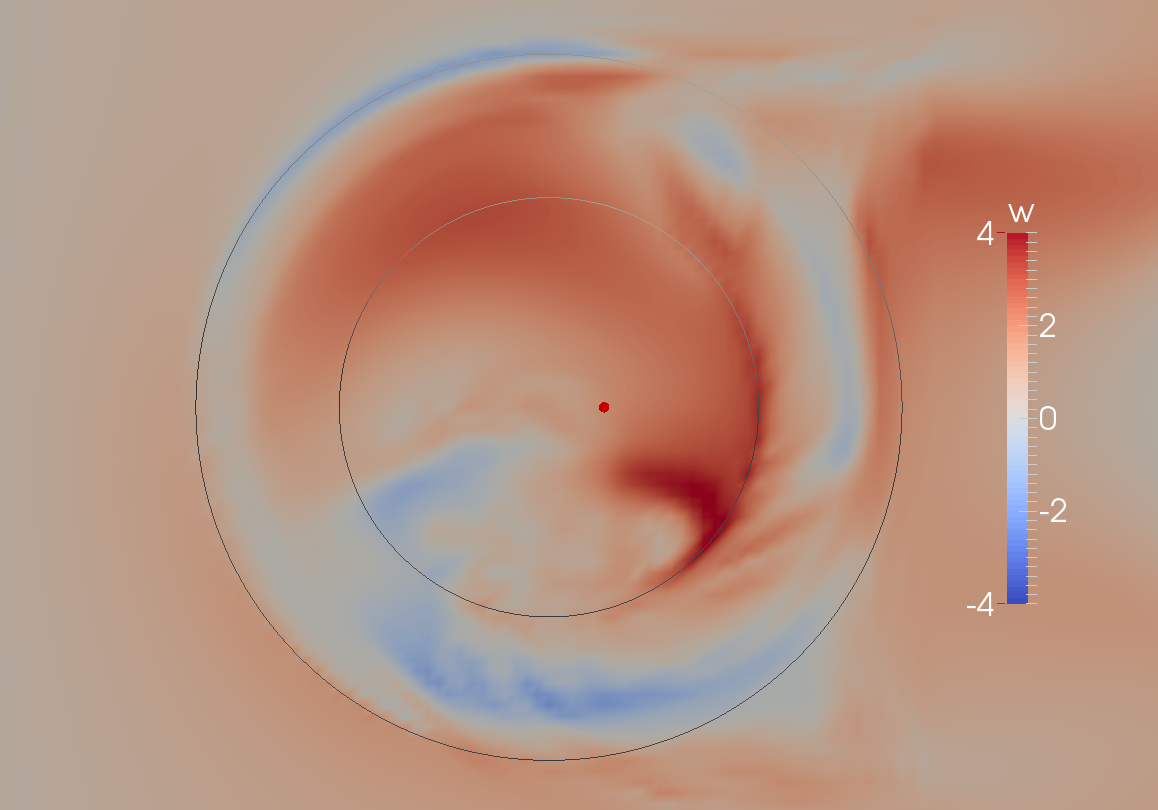
\includegraphics[width=.47\linewidth]{figs/wind_w}
 %\caption{Vertical Velocity}
 % \label{fig:vz-wind}
 \\
  \centering
  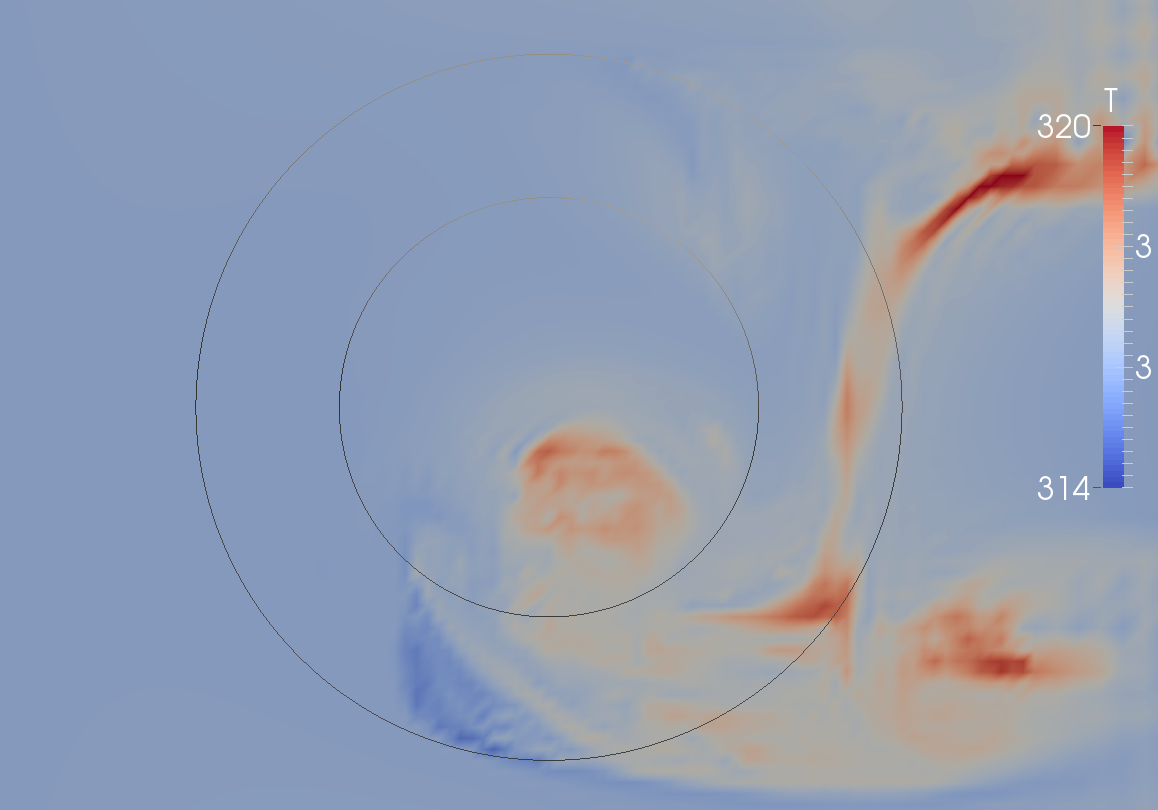
\includegraphics[width=.47\linewidth]{figs/wind_t}
 \hfill
  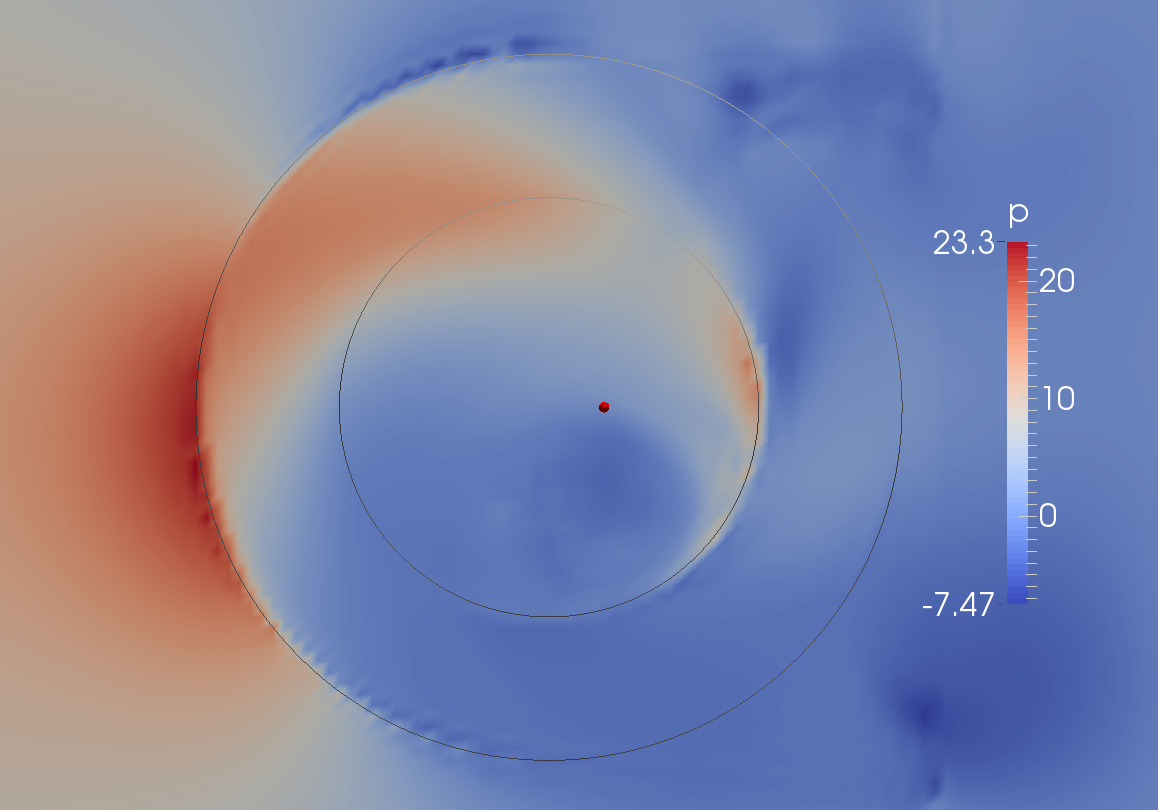
\includegraphics[width=.47\linewidth]{figs/wind_p}
  %\label{fig:p-wind}
 \caption{Time averaged horizontal slices taken at the height of the
 vanes for the wind cases. The streamwise velocity shows a large
 penetration in the region where the vanes are not blocking, and in the
 other regions the flow is blocked and flows around. The vertical
 velocity is disorganized and does not show the ``two cell'' structure
 as in the thermal-only cases.  Note that an
 off-center thermal plume is visible, as well.  } 
 \label{fig:wind-hor}
\end{figure}


Horizontal slices of the azimuthal and vertical velocities, and the 
temperature and pressure fields are shown in
Figure~\ref{fig:vz-wind-vert}\todo{bring me back}. The freestream
velocity is traveling from left to right at 5 m/s, which was set based
on ambient velocity measurements made by the experimental team from the
field. While the structure is undoubtedly different than the
thermal-only cases shown previously, we can nevertheless see that a
thermal plume is forming along with a rotating velocity structure. In
general the wind cases are more disorganized, with less obviously
visible coherent structure. Notice however that the magnitude of
velocities are several times larger than in the thermal-only cases, and
the kinetic energy flux through the vanes is also significantly higher.   

%
% vertical
%

% \begin{figure}[htb]

%  \begin{subfigure}{.5\textwidth}
%   \centering
%   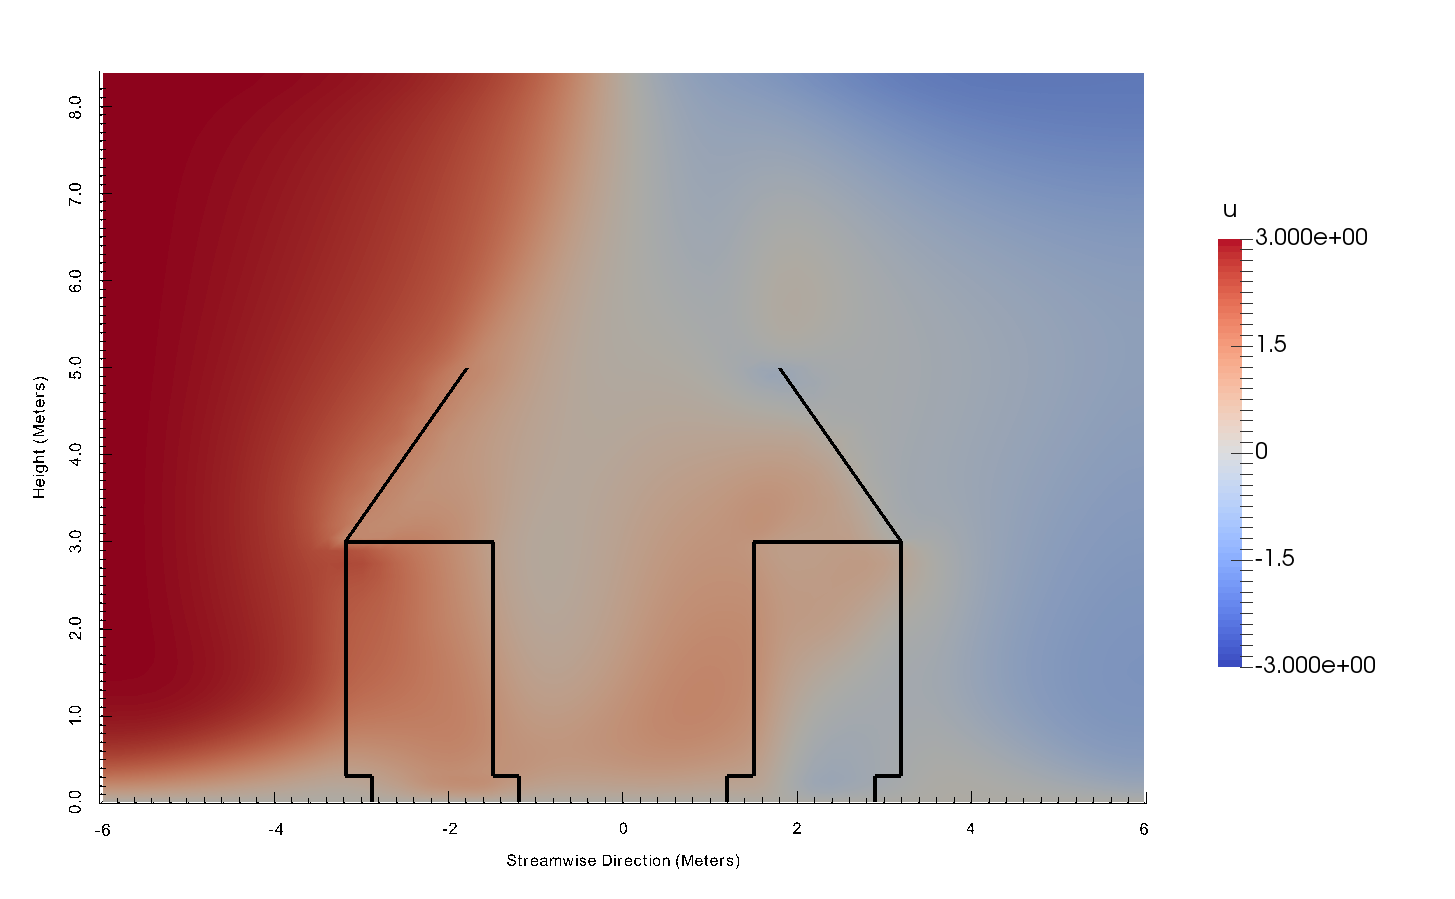
\includegraphics[width=.75\linewidth]{figs/wind_u_vertical}
%   \caption{Streamwise}
%   \label{fig:vt-wind-vert}
%  \end{subfigure}%
%  \begin{subfigure}{.5\textwidth}
%   \centering
%   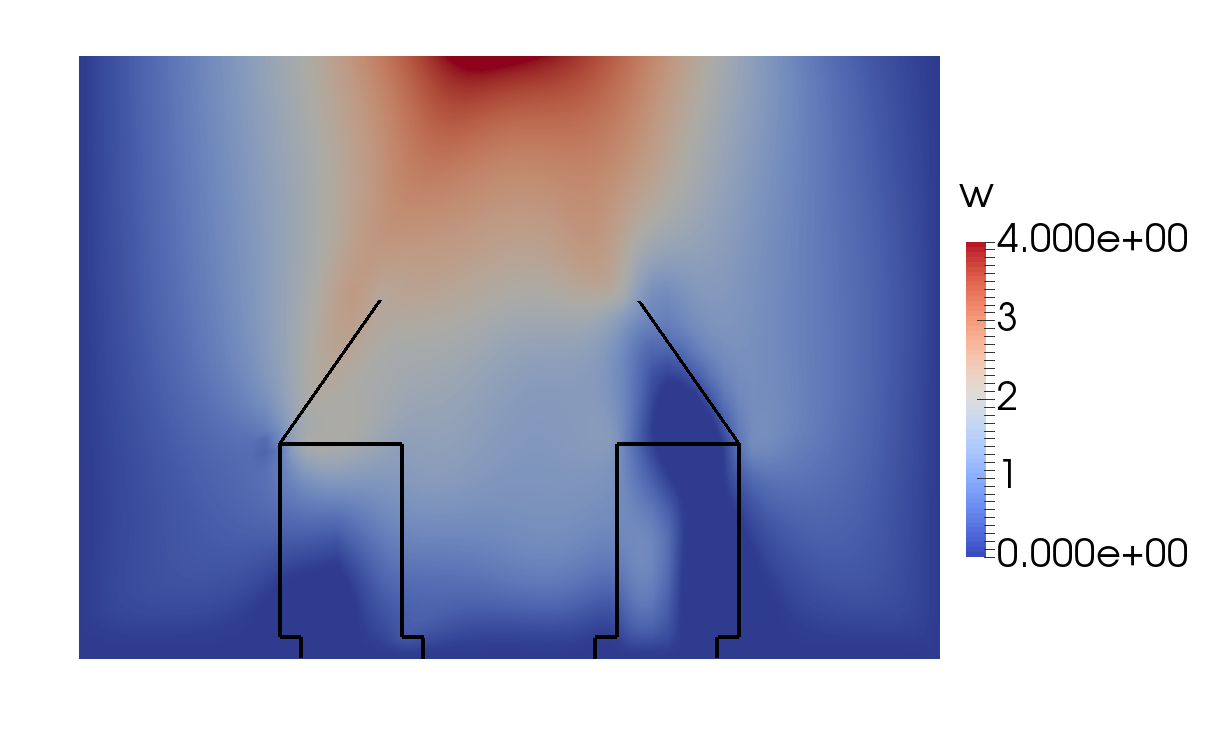
\includegraphics[width=.8\linewidth]{figs/wind_w_vertical}
%   \caption{Vertical Velocity}
%   \label{fig:vz-wind-vert}
%  \end{subfigure}%


%  \begin{subfigure}{.5\textwidth}
%   \centering
%   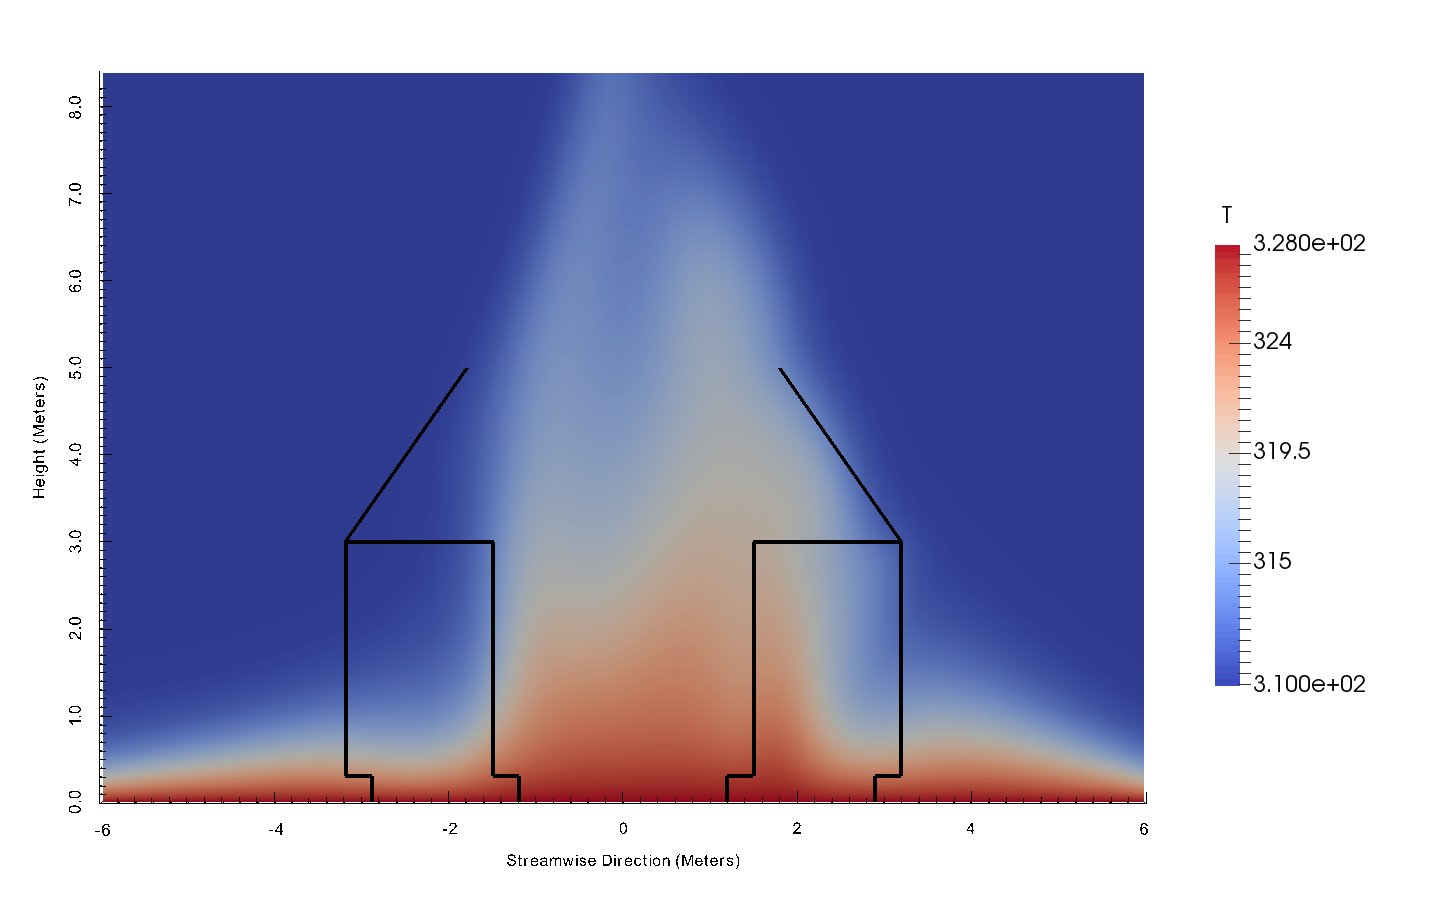
\includegraphics[width=.85\linewidth]{figs/wind_t_vertical}
%   \caption{Temperature}
%   \label{fig:t-wind-vert}
%  \end{subfigure}%
%  \begin{subfigure}{.5\textwidth}
%   \centering
%   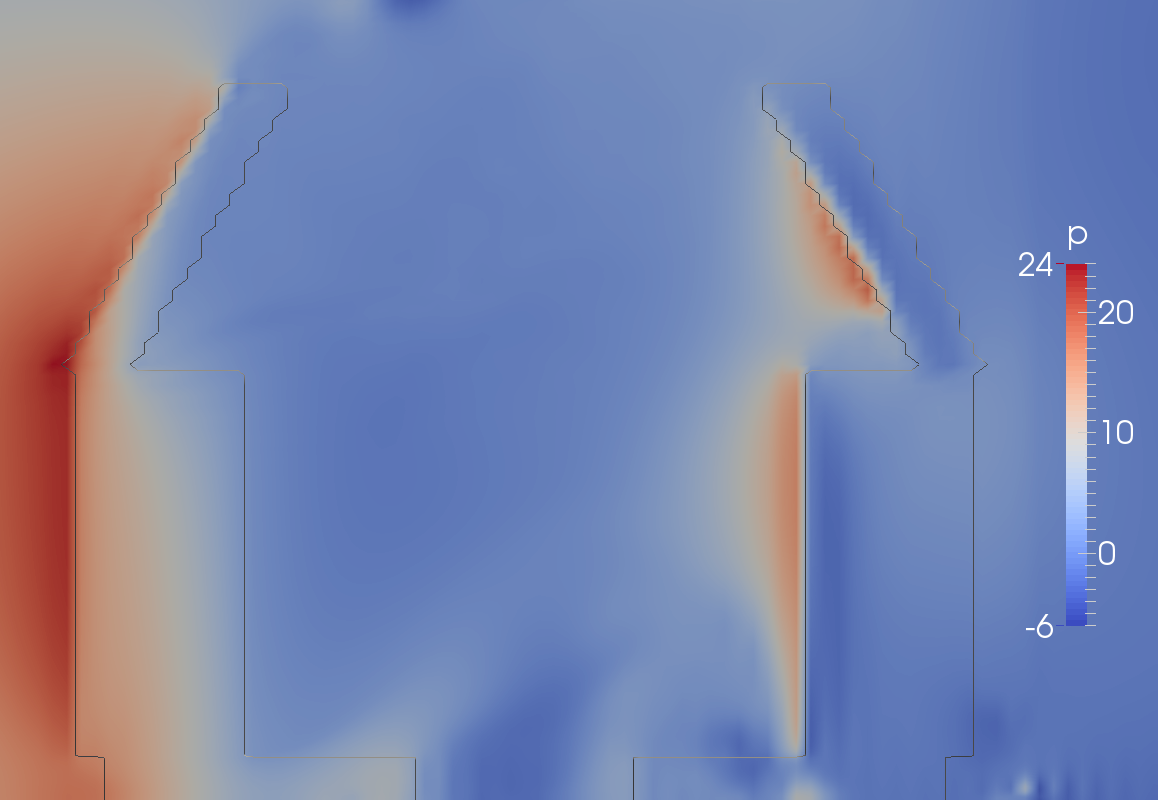
\includegraphics[width=.75\linewidth]{figs/wind_p_vertical}
%   \caption{Pressure}
%   \label{fig:p-wind-vert}
%  \end{subfigure}%

%  \caption{Time averaged vertical slices from the center of the device
%  for the wind cases. A great deal of flow is radially entrained by the
%  first tier of vanes, consistent with the approach proposed in
%  Figure \ref{fig:cartoon_vanes}. 
%  Notice that while the temperature field appears to
%  be quite modest, this is due to the fact that the thermal column is not
%  well centered. The full column is quite visible in Figure
%  \ref{fig:field_real}.}  
%  \label{fig:wind-ver}
% \end{figure}

The vertical slices are shown in Figure~\ref{fig:wind-ver}. In this
case, the lower tier of vanes are where the majority of flow is 
entering the center of the apparatus, while the second tier of vanes are
blocking the ambient wind and providing protection for the vortex column. 

The thermal plume is significantly less
visible than in the thermal-only cases. While the
thermal-plume is necessarily weaker relative to the wind, some of this
is also due to the plume no longer being directly centered in the
flow. The plume is more visible using isocountors to render a
three-dimensional surface. 
To visualize the difference between the vertically varying ambient
temperature and the warmer thermal plume, we use the potential
temperature, defined as,\todo{kill this?} 
\begin{equation}
  \tau(x,y,z) = T(x,y,z) -T_{\text{in}}(z) 
   \label{eqn:tau}
\end{equation}
where $T_{\text{in}}$ is the inflow temperature, described
in Chapter \ref{sec:bc}. In this way the background potential
temperature is nearly zero, and larger values represent deviations from
the base flow temperature. The isocountour of a three Kelvin is 
shown in Figure~\ref{fig:field_real}. This value was selected as
it was noted as sufficient for formation of a dust devil by
Sinclair~\cite{Sinclair1969}. It is clear from the image that a 
strong thermal column does exist even in the $5 m/s$ wind cases. 

%
% tiso
%
  \begin{figure}[!htb]
   \begin{center}
    \includegraphics[width = 12 cm]{figs/t_iso}
    \caption{Iso-contour of the thermal plume. Here, the isocontour is
    labelled by the potential temperature, $\tau$, as defined in
    Equation \ref{eqn:tau}. A strong thermal column has visibly formed. The
    figure is colored by the streamwise velocity, and shows the thermal
    column also has rotation.} 
    \label{fig:field_real}
   \end{center}
  \end{figure}

\section{Optimization}

In this section results from a representative optimization
in a thermal-only case are discussed, to demonstrate the optimization 
process employed so far. This is a typical mode of scientific and
engineering inquiry, where a hypothesis regarding system operation is
developed, followed by testing of the hypothesis, and further
iterations.  

This series of simulations are all runs with different system
configurations conducted in a common ambient scenario, that of the
unsteady thermal-only simulations described in Chapter~\ref{sec:bc}. 

Our objective is to maximize the energy that can be 
extracted from the synthetic dust devil. As a surrogate to this
quantity, consider the kinetic energy flux through a horizontal plane
near the top of the vanes, where a turbine will ultimately be
placed. This is a surface integral~\cite{landau1959fm},

% flow.io is awesome
% https://support.draw.io/questions/2949135/how-to-use-mathematical-typesetting
%
%
%https://www.draw.io/?url=https%3A%2F%2Fjgraph.github.io%2Fdrawio-diagrams%2Fdiagrams%2Fmath.xml
%


%% \begin{equation}
%%  \dot E = -\oint \rho \textbf{v}(\frac{1}{2}v^2 + e) \cdot d \textbf{f}
%% \end{equation}
%% where $e$ is the internal energy. % and $d\textbf{f}$ the. 
%% For our problem, we consider an incompressible fluid flowing through a
%% flat horizontal region interior to the vanes in the x-y plane, which
%% results in, 

 \begin{equation}
  \dot{ \text{KE}} = -\frac{\rho }{2} \int V_z (V_{\theta}^2 + V_z^2 ) dA.
 \end{equation}

\begin{figure}[htb]
 \centering
 \includegraphics[width=.75\linewidth]{figs/opt_plot}
 \caption{This plot diagrams the improvements to the calculated flux for  
 each iteration of system configuration in the thermal-only optimization
 effort. Every iteration is labeled by design change. This list
 only highlights the accepted improvements, and the numerous runs of a
 particular parameter configuration that yielded inferior power output
 are not shown. }
 \label{fig:opt_plot}
\end{figure}


% \begin{figure}[htb!]
%  \begin{subfigure}{.5\textwidth}
%   \centering
%   \includegraphics[width=.75\linewidth]{figs/before_vanes}
%   \caption{Vanes before optimization}
%  \end{subfigure}%
%  \begin{subfigure}{.5\textwidth}
%   \centering
%   \includegraphics[width=.8\linewidth]{figs/after_vanes}
%   \caption{Vanes after optimization}
%  \end{subfigure}%
%   \caption{Can we do this}
%  \label{fig:vt-wind-vert}
% \end{figure}\todo{need better figure}




\begin{figure}[htb]
  \centering
 \includegraphics[width=.45\linewidth]{figs/before_opt}
 \hfill
 \includegraphics[width=.45\linewidth]{figs/after_opt} \\
  \caption{These are vertical slices taken at the center of the vanes of
 the vertical velocity taken before and after the numerous optimizations
 of the turning vanes detailed in Figure \ref{fig:opt_plot}. In the
 original (left image), the flow produces a narrow plume. In the second
 (right figure), the flow shows stronger vertical velocities in a much
 larger and more organized vortex. The flow has also transitioned into a
 ``two-cell'' structure akin to that observed in the naturally occuring
 phenomena as discussed in Chapter \ref{subsec:phenomena}}
  \label{fig:opt_flow}
\end{figure}


Using the kinetic energy flux as an objective, the vane geometry has
been optimized. Over approximately tens of iterations, we have
increased the kinetic energy flux by a factor of 88 relative to the
baseline. 

\begin{figure}[htb]
 \centering
 \includegraphics[width=0.75\linewidth]{figs/optimization_flow}
 \caption{A flowchart detailing the optimization heuristic. $\eta$ is
 representative of any SoV geometric parameter, such as the vane angles,
 vane height, cone contraction, etc. $\epsilon$ is a small perturbation
 to the base state, which is not randomly selected but typically is a
 small fraction of the base value. }
 \label{fig:opt_image}
\end{figure}


%Results of several of these iterations are documented in
%Figure \ref{fig:opt_plot}. 
Major adjustments to design in the the vane
shape and angles were made to obtain this improvement. Before and after
images are shown in Figure~\ref{fig:vt-wind-vert}. During this
optimization the 
qualitative character of the solution changed substantially, changing
from a mild upward flow with little rotation to a strongly organized
vortex with a downward central flow and strong azimuthal
velocities. Before and after vertical slices are shown in
Figure~\ref{fig:opt_flow}. Nevertheless, with a peak energy flux for the
final iteration of less than one hundred Watts, significant further 
optimization is necessary for this system to be viable for use as an 
energy production system. This naturally leads to the next section,
which is a discussion of the proposed research campaign. 

\section{The Effect of the Wind}
\label{sec:wind_impact}

% Regarding question number 2, you want to optimize the lift vector (see
% the figure below).  For the figure, pretend you are sitting to the side
% of the turbine as the blade is moving up.  We want the L vector to be as
% close to vertical as possible (in the useful torque direction that will
% pull the blade up).  In order to do that you need to optimize the
% Lift/Drag, but you also need to minimize the downwash (Utheta0 and Uz0
% vectors) as the downwash will turn the lift vector away from the useful
% torque direction.   Atkins and Liebeck show how to minimize the downwash
% at a given design condition for a given a set of optimum airfoils.  You
% can directly solve for blade twist and planform to make sure downwash is
% minimized and each airfoil is at its Max L/D, but this often gives rotor
% designs that are not robust and structurally infeasible.
% However, it will give you an idea of what the ideal blade looks like at
% different conditions and then you can work to find a more robust
% solution and add structural constraints as well.   

thermal vs wind, be sure to mention thermal doubles energy output

\section{Energy Scaling with Vortex Size}

ugh, what can we do here?


\section{Comparison's between Natural and Synthetic Dust Devils}

Show rankene. 

This is qualitatively similar to simulated tornado velocity
profiles\ref{nolan1999structure}. 



Do we want to talk about hurricanes?


 required is coupling the interior vortex model to a
 boundary layer model that is coupled to a model of surface heat flow
 through soil or sand. The rate limiting factor is bound to be the
 diffusion of heat through a thin super-heated surface layer of
 the surface\cite{emm_comm}.   

In fact, a study of this nature has been performed with current
atmospheric models\cite{emanuel2008hypothesis}, but still relied upon
moisture source term modeling rather than sensible heat flux.   

\chapter{Conclusions}
\label{sec:conclusions}

The objective of this research project is to provide a definitive
assessment of the technological feasibility of the entire synthetic
columnar vortex concept as a means of generating usable energy. In the 
previous sections outlined the present state of the
simulation capability. In doing so, we have discussed the physics that
influence dust devils formation, our particular mathematical
models for the ambient conditions, as well as the SoV vanes, cone and
turbine. We summarized the numerical discretizations used, the software
stack and the calibration, verification and validation of these
components. The purpose of these sections was to communicate
two major points. The first is that an accurate, verified and
validated simulation capability has been developed that can quickly
investigate a wide variety of system and scenario settings at a modest
computational cost. The second point is that we have developed
heuristics that permit optimization of any baseline SoV configuration to
a local maximum of energy production, as measured by kinetic energy flux
through the top of the SoV vanes.  

These two points justify the proposed course of work, which is to
explore a large space of possible system configurations
and geometries to discover the globally optimal structure
of the SoV apparatus. Coupled with the scaling analysis presented in
Section \ref{sec:physics}, we will then be able to predict the
conditions (if any) under which the SoV apparatus will be
technologically feasible. This will lead to investigating the physics of the
apparatus, to assess how closely the synthetic dust devils mimic the
natural variety. The proposed research is designed to
assess feasibility, and it is not expected that actual experimental
validation will accompany the computational results. Furthermore, it
must also be emphasized that feasibility is focused on
technical viability, namely energy produced by the apparatus,
and will not include an economic assessment. In other words, it is
possible that the SoV will produce energy, but the design required to do
is prohibitively expensive, and therefore not economically competitive
with existing technologies. The following is a proposed program of simulations 
designed to explore a wide configuration space. This focuses on
optimization for the cone, turbine and vanes. 

%
% vane optimization
%
%% \large
%% \begin{center}
%% \begin{table}[h]
%%  \centering
%%   \begin{tabular}{| l | c | l |}
%%     \hline
%%     Parameter & Description & Range \\
%%     \hline
%%     $\theta^{\text{t}}_{\text{min}}$ & Starting, minimum angle of the
%%        top tier & ( 0 - $\theta^{\text{t}}_{\text{max}}$ ) \\
%%     $\theta^{\text{t}}_{\text{max}}$ & Ending, maximum angle of the top
%%        tier & ( 0 - 90 ) \\
%%     $\theta^{\text{b}}_{\text{min}}$ & Starting, minimum angle of the
%%        bottom tier & ( 0 - $\theta^{\text{b}}_{\text{max}}$ ) \\
%%     $\theta^{\text{b}}_{\text{max}}$ & Ending, maximum angle of the
%%        bottom tier & ( 0 - 90 ) \\
%%    $\gamma^t$ & Rate of curving, vane top tier & ( 0 - 3 ) \\
%%    $\gamma^b$ & Rate of curving, vane bottom tier & ( 0 - 3 ) \\
%%    $1 - (r_{\text{min}} / r_{\text{max}})^{\text{t}}$ & Length of the top
%%        tier vane & ( 0 - 1 ) \\
%%    $1 - (r_{\text{min}} / r_{\text{max}})^{\text{b}}$ & Length of the
%%        bottom 
%%        tier vane & ( 0 - 1 ) \\
%%    $H^b/H^t$ & Ratio of heights between bottom and top tiers & ( 0 -
%% 	   0.5 ) \\ 
%%    $D/H$ & Ratio of apparatus diameter and total vane height & ( 0.5 -
%% 	   5.0 ) \\ 
%%     \hline
%%   \end{tabular}
%%   \caption{Vane Optimization Parameters.}
%%   \label{tab:vane}
%% \end{table}
%% \end{center}
%% \normalsize\todo{keep table?}

The three cone parameters we propose to optimize are shown in Table
\ref{tab:cone}. We expect to optimize the cone after the bottom and top
tiers are adjusted. For the cone, we expect the height, maximum diameter
and inner exit diameter to all impact the flow. While it is not known
what form the ideal cone geometry will take, our expectation is that the
cone plays at least two important roles. The first is acting as a
converging nozzle for the flow, increasing the vertical and azimuthal
velocity as it exits out the top of the device. In the wind, the cone
also acts as a shield, preventing the high velocity freestream flow from
disrupting the vortex before it has run through the turbine. 

%
% cone optimization
%
\large
\begin{center}
\begin{table}[h]
 \centering
  \begin{tabular}{| l | c | l |}
    \hline
    Parameter & Description & Range \\
    \hline
    $H_C/D_C$ & Ratio of the height of the cone versus the cone diameter & ( 0 - 2.0 ) \\
    $D_{\text{C}}/D$ & Ratio of the cone diameter versus the system
       diameter & ( 0.5 - 1.5 ) \\
    $D_{\text{out}}/D_C$ & Ratio of the cone exit diameter versus the
       cone diameter & ( 0.25 - 1.0 ) \\ 
    \hline
  \end{tabular}
  \caption{Cone Optimization Parameters.}
  \label{tab:cone}
\end{table}
\end{center}
\normalsize

The turbine parameters to be optimized are shown in Table
\ref{tab:turbine}. In addition to these configuration parameters, the
location of the turbine will likely need to be optimized to be centered
on the vortex, which may not be centered inside the vanes due to
asymmetric effects of wind, vane geometry, etc. 

%
% turbine optimization
%
\large
\begin{center}
\begin{table}[h]
 \centering
  \begin{tabular}{| l | c | l |}
    \hline
    Parameter & Description & Range \\
    \hline
    $N_B$ & Number of blades & ( 1 - 12 ) \\
    $I$ & Moment of inertia & ( 1 - 12 ) \\
    $r_B/r_{\text{min}}^t$ & Radius of blade versus the inner radius of
       the top tier vanes & ( 0 - 1 ) \\
   $H_B/H$ & Height of the turbine blades versus system height & ( 0 - 1.2 ) \\
    \hline
  \end{tabular}
  \caption{Proposed Turbine Optimization Parameters.}
  \label{tab:turbine}
\end{table}
\end{center}
\normalsize

The possible configuration space for the vanes is much larger. 
Presently, the workflow consists of weekly calls with the experimental
team to discuss possible system designs, which typically consist of vane
sketches or drawings. One such proposed design is shown in Figure
\ref{fig:sketch}.  These vanes are highly asymmetric with variation in
the length and curvature as a function of spatial location. Furthermore,
in this design the down wind side of the apparatus is enclosed by a
solid cylindrical wall.  While the vane representation outlined in
Section \ref{subsec:vane} is expected to be sufficiently general to support a
wide variety of vane configurations, it is not at this time clear what
form of parameterization for vane angle is sufficiently general to
support this exploration, and so a table like that for the cone and
turbine is not yet available. At present the expectation is to proceed
with this conceptual phase to generate a wide  range of possible
configurations. The designs that have initially promising results will
then be optimized similar to the examples outlined in Section
\ref{sec:results}, where new parameter values are 
introduced, a run is performed, and then the output is postprocessed and
evaluated before the process begins again. In this way it is not
infeasible to expect that several hundred optimization runs can be
performed. 
%The next subsection also briefly outlines a proposal to
%investigate algorithmic optimization on these designs.  

\begin{figure}[htb]
 \centering
 \includegraphics[width=.75\linewidth]{figs/top}
 \caption{This is an example image of a proposed vane design. The lines
 indicate the vane curvature and solid surfaces. Sketches and diagrams
 such as this  are typically generated by various members of the
 team. The vane surface is then instantiated as a region of forcing as
 detailed in Section \ref{subsec:vane} and then simulated. If the
 initial results are promising, then further exploration of that
 configuration may be pursued.} 
 \label{fig:sketch}
\end{figure}



% Table \ref{tab:vane} lists the proposed optimization parameters for the
% vanes. We propose nine parameters to optimize for the
% vanes. $\theta^{\text{t}}_{\text{min}}$ and
% $\theta^{\text{b}}_{\text{min}}$ are the top and bottom tier minimum
% angles. This is essentially the starting (and minimum) angle for the curved
% vanes. Preliminary investigations have given no indication that the
% bottom tier is receptive to anything but a fully radial angle
% (e.g. $0^{\circ}$). For the top tier, however, a non-zero
% $\theta_{\text{min}}$ has been found to increase the kinetic energy
% flux. For both of the maximum angles we have reasonable starting
% points. Previously, we have found that a larger angle at the bottom tier
% is ideal, as it serves to ``spin-up'' a small core region.

% We have less strongly informed prior expectations of reasonable values
% for the rate of curvature, $\gamma$, the ratio of heights between the
% top and bottom tiers ($H^b/H^t$) as well as the lengths of the
% vanes. The generated flux is certainly sensitive to $\gamma$, but
% optimal value is certainly not known. Likewise, while we have operated
% with shorter vanes lengths on the top than the bottom, as well as a
% shorter height, we are not certain that these configurations are
% remotely optimal. Finally, for $D/H$, the ratio between the apparatus
% diameter and total vane height, we have only operated near a ratio of
% 1.0. However, as noted in \cite{ROG:ROG1635}, ``Most dust devils are at 
% least 5 times higher than they are wide''. While increasing the height
% of the apparatus would greatly increase the cost and inaccessibility of
% the device for maintainance, this indicates that it is necessary to
% examine the dependence of energy produce by the vortex at greater system
% heights. We expect to increase beyond this aspect ratio of $\approx 1$
% towards the naturally occuring ratio of 5. If this is found to greatly
% enhance energy output, we will then consider even larger
% ratios.\todo{add image}
%
% need to expand this to discuss huge space of vanes
% add image too?
%



%\subsection{Risks and Challenges to the Optimization Efforts}

%% A challenge inherent to this optimization effort is that while the
%% principle quantity of interest is the kinetic energy flux, we also seek
%% to use these runs to shed light on the mechanisms by which the apparatus
%% configuration dictates the flow. In other words, we are trying learn
%% more than \textbf{which} configurations optimize the flow, but also 
%% \textbf{why} they do so. 

% This presents an programmatic challenge, as
% optimization will involve additional analysis and postprocessing at each
% iteration.  

%
% how many runs are we capable of performing, realistically
% largely obsolete!

% An additional challenge is the computational expense of each run. 
% Each parameter exploration requires approximately 12 wall-clock hours to run
% the simulation for a sufficient time to pass any initial transient in
% the solution and then permit adequate statistical averaging at steady
% state. Runs generally require approximately 264 processors on Lonestar
% (for example) and therefore the cost of a forward run is $\approx 3,200$
% core hours. Our overall compute budget will likely be between one hundred
% thousand to one million core hours. In other words, our present
% computational budge will support running between roughly 30 to 300
% instances for our parameter sweeps. While this is not insubstantial, this
% is not a sufficient number of evaluations to support formal
% optimization algorithms. While we admittedly do not, \textit{a priori},
% know the number of iterations necessary to solve the system, as it is
% non-linear, our expectation is that thousands of forward solves would be
% necessary. Using higher order methods could reduce the number of
% iterations, but gradient and derivative information is difficult to
% access, as solving the adjoint problem is expensive for unsteady systems. 
% Thus, while any individual run is relative inexpensive, we do not expect
% to be able to mount an exhaustive campaign to formally optimize the
% configuration given the dimension of the parameter space and the
% structure of the problem. 

%
% introduce concept of subdomains
%

% Furthermore, the time requires to perform this simulation campaign could
% be greatly reduced if several problems were to be undertaken in
% parallel. This ``divide and conquer'' approach requires subdividing the
% optimization effort into several ``subdomains''. 
% The problem is nonlinear, and so some of the parameters are coupled and
% cannot be easily optimized independent of each another, as adjustments
% to one impact the desired value of the other. 
% We propose to subdivide the vanes into upper and lower tiers, optimize
% them individually, and then perform rudimentary sensitivity checks to
% ensure that the coupled product does in fact represent a near optimal
% flux output. We further expect that the remaining parameters in the
% vanes, namely $H^b/H^t$, $D/H$ are amenable to optimization independent
% of the particular parametric configuration of the vane tiers. 

% The subdomains for the vanes are are summarized in Table
% \ref{tab:opt}. This neatly divides the vane optimization effort into
% three independent problems with 4 or fewer parameters each.

% \begin{center}
% \begin{table}[h]
%  \centering
%   \begin{tabular}{|l | l | l |}
%    \multicolumn{3}{c}{Subdomains} \\
%     \hline
%    Top Tier & Bottom Tier & Misc. \\
%    \hline
%    $\theta^{\text{t}}_{\text{min}}$ & $\theta^{\text{b}}_{\text{min}}$ &
%        $H^b/H^t$ \\
%    $\theta^{\text{t}}_{\text{max}}$ & $\theta^{\text{b}}_{\text{max}}$&
% 	   $D/H$ \\ 
%    $\gamma^t$ & $\gamma^b$ & \\
%    $1 - (r_{\text{min}} / r_{\text{max}})^{\text{t}}$ & $1 -
%        (r_{\text{min}} / r_{\text{max}})^{\text{b}}$ & \\
%    \hline
%   \end{tabular}
%   \caption{Vane optimization parameters, divided into parallelizable
%  subdomains.} 
%   \label{tab:opt}
% \end{table}
% \end{center}

\subsection{Proposed Timeline}

%
% timeline
%
A timeline for the proposed work is presented in Table
\ref{tab:prop}. The date of each bullet is the planned completion of the
deliverable. Bullets items in black are required, while those in blue
are optional, and do not need to be completed to ensure the
success of this project. 

% 
% can we optimize? DAKOTA
% 
% We propose to investigate algorithmic optimization as a tool to discover
% locally optimal system configurations. 
% This will take the form of using either the DAKOTA\cite{adams2013dakota}
% or TAO\cite{tao-user-ref} libraries. These libraries have suites of
% algorithms for non-linear optimization problems without gradient
% information (derivative-free optimization, such as Nelder-Mead or downhill simplex methods). 
% Evaluating the results of the most
% appropriate ``out of the box'' available optimization algorithm on a
% small test problem will provide an opportunity to ensure that our
% expectations on the number of iterations necessary for formal
% optimization of our problem are reasonably correct. 
% We propose these two libraries because DAKOTA is well-known as a library
% with extensive ``black-box'' optimization support, and TAO is already
% made available through pre-existing libMesh dependencies. Should the
% test problem discover that algorithmic optimization is a viable option,
% we will consider using this approach for optimization of the
% configuration. 

%
% short summary of tasks
%

The first bullet in Table \ref{tab:prop} provide
estimated ending dates for the exploration of the configuration space. 
We have rapidly iterated 
through these optimization efforts over the course of several
months, and are nearly converged on a final design. 
The second bullet relates to the the final verification of the turbine, to ensure
this functions properly. 
At this time we will proceed with ``coupling tests'' to 
ensure that the parameters are indeed still appropriate. For example,
after having optimized the turbine parameters, it may be necessary to
perturb the lower tier vane parameters to ensure that the selected set
is nearly optimal even with the addition of a turbine. 

%
% probably ok below:
%
The third bullet is the expected deadline to provide the results of our
computational simulation efforts to the experimental group in late
Spring/early Summer of 2016 so that they can use this information in the
design of the system to be used for the Arizona field tests in Summer,
2016. The date of the actual field test has not yet been set and may change. 

As mentioned in the fourth item, it is possible that this
project will permit some glimpses  
at the fundamental processes underlying the naturally dust devil
phenomena. To accomplish this, the synthetic dust devils must be
compared to data from the naturally occuring variety,  with some
appropriate scaling. While it is not a significant component of the
proposal, this and several simple investigations into related phenomena
such as tornados and hurricanes will also  be investigated. A literature
review of the physics of general cyclonic structures and any observed
intensification mechanisms may provide hints of the geometries 
by which the flow is intensified, and why. 

Given our previous experiences, we do not anticipate a rich validation data set 
to be available after the field test. Nevertheless, we will postprocess any and all
available data from this event in order to assess the reliability of the computational
modeling efforts. 

Finally, we anticipate a detailed accounting of the entire project as
the final deliverable. We expect that all of the investigations detailed 
above will result in several publications, as well. 

%
% itemize tasks
%
% In summary, in addition to the preliminary results, several tasks will be
% accomplished  to fulfill the goals of this project:

% \begin{itemize}
%  \item validate turbine
%  \item numerous optimization runs
%  \item best guess of ideal run (possible field run)
%  \item feasibility study?
% \end{itemize}

\begin{center}
\begin{table}
\caption{Timeline of proposed work. Bullets are dates of planned
 completion of deliverables. Black items are requisite, blue optional.}
\centering
\begin{minipage}[t]{.7\linewidth}
\color{black}
\rule{\linewidth}{1pt}
\ytl{April 2016}{Conclude parameter sweeps and optimization of apparatus}
\ytl{April 2016}{Turbine actuator-disk verification, validation and prediction}
\ytl{May 2016}{Proposed configuration and predictions for experimental
 team}
\ytb{July 2016}{Comparisons between synthetic and natural dust devil physics}
\ytl{Aug 2016}{Validation against 2016 field data}
%\ytl{Aug 2016}{SoV feasibility assessment}
\ytl{Fall 2016}{Doctoral dissertation writing}
\bigskip
\rule{\linewidth}{1pt}%
\end{minipage}%
\end{table}
\label{tab:prop}
\end{center}

% \subsection{Additional Investigations}

% % 
% % control for inter unit spacing
% % 
% In addition to the system configuration, it would be interest to consider the
% effect of local conditions on SoV performance. Characterizing the impact
% of variations in ambient conditions on the SoV will guide the
% commercialization strategy of the product, by determining optimal
% install locations across the country. It is therefore desirable to have
% models that are capable of accounting for variation in field conditions,
% such as solar input, cross-winds and topography. Furthermore, it is
% expected that large ``farms'' of SoVs (akin to the wind and solar farms
% for wind turbines and photovoltaics, respectively) may be used by
% commercial or utility-scale energy generation. For this to be
% effective,  the inter-unit spacing must also be optimized, as a single
% SoV collects from a large area. These computations will guide
% commercialization planning, where decision-makers will need to assess
% optimum unit size, spacing, and geographic location for utility-scale
% deployment.   


%%%%%%%%%%%%%%%%%%%%%%%%%%%%%%%%%%%%%%%%%%%%%%%%%%%%%%%%%%%%%%%%%%%%%%
% Appendix/Appendices                                                %
%%%%%%%%%%%%%%%%%%%%%%%%%%%%%%%%%%%%%%%%%%%%%%%%%%%%%%%%%%%%%%%%%%%%%%
%
% If you have only one appendix, use the command \appendix instead
% of \appendices.

\appendices
%%\appendix

\chapter{Derivation of the Stabilization and Weak Formulation}
\label{sec:derivation}

Here the mathematical models summarized in \autoref{sec:model} are derived.
While the first two sections containing the Navier--Stokes and Favre-averaged
Navier--Stokes equations are classical and straightforward, the derivations are
provided to document the few peculiar constitutive choices as well as to
unambiguously fix nomenclature.  The third section documents a new
spatiotemporal homogenization approximation by \citet{Topalian2014Spatiotemporal}.
%
Dimensional equations are employed throughout this appendix.  The final
dimensional summary in each of the following subsections is nondimensionalized
to arrive at the formulations used in the main body of the dissertation.

\section{The Governing Equations}

\subsection{Conservation Laws}

%\subsubsection{Reynolds transport theorem}
Consider a time-varying control volume $\Omega$ with surface
$\partial\!\Omega$ and unit outward normal $\hat{n}$.  For any
scalar, vector, or tensor field quantity
$T$, Leibniz' theorem states
\begin{align}
  \label{eq:rtt}
  \frac{d}{dt}\int_{\Omega(t)}T(x,t)\,dV
  &=
  \int_{\Omega}\frac{\partial\!}{\partial\!t}T\,dV
  +
  \int_{\partial\!\Omega} \hat{n}\cdot{}w T\,dA
  =
  \int_{\Omega}\frac{\partial\!}{\partial\!t}T+\nabla\cdot{}wT\,dV
\end{align}
where $w$ is the velocity of $\partial\!\Omega$.  When $\Omega$ follows
a fixed set of fluid particles, $w$ becomes the fluid velocity $u$.

%\subsubsection{Conservation of Mass}
Since mass $M=\int_{\Omega} \rho\,dV$
and mass conservation requires $\frac{d}{dt}M=0$,
\begin{align}
  0 = \frac{d}{dt}M
  = \frac{d}{dt}\int_{\Omega} \rho\,dV
  =
  \int_{\Omega}\frac{\partial\!}{\partial\!t}\rho+\nabla\cdot{}u\rho{}\,dV.
\end{align}
Because the result holds for any control volume, locally it must be true
that
\begin{align}
  \label{eq:cons_mass}
  \frac{\partial\!}{\partial\!t}\rho+\nabla\cdot\rho{}u &= 0.
\end{align}

%\subsubsection{Conservation of Momentum}
Separating total force into surface forces and body forces,
\begin{align}
  \sum{}F
  &=
     \int_{\partial\!\Omega} f_s \, dA
   + \int_{\Omega} f \, dV
  =
     \int_{\partial\!\Omega} \sigma \hat{n} \, dA
  +  \int_{\Omega} f \, dV
  =  \int_{\Omega} \nabla\cdot\sigma + f \, dV
\end{align}
where $\sigma$ is the Cauchy stress tensor.  From linear momentum
$I=\int_{\Omega} \rho{}u\,dV$ and its conservation $\frac{d}{dt}I=\sum{}F$,
\begin{align}
    \int_{\Omega}\frac{\partial\!}{\partial\!t}\rho{}u
  + \nabla\cdot(u\otimes{}\rho{}u)\,dV
&= \int_{\Omega} \nabla\cdot\sigma + f \, dV
.
\end{align}
As the control volume may be arbitrary,
\begin{align}
  \frac{\partial\!}{\partial\!t}\rho{}u + \nabla\cdot(u\otimes{}\rho{}u)
&= \nabla\cdot\sigma + f
.
\end{align}
Lastly, separating the pressure $p$ and viscous contributions $\tau$ to
the Cauchy stress tensor so that $\sigma = -p I + \tau$,
\begin{align}
\label{eq:cons_momentum}
\frac{\partial\!}{\partial\!t}\rho{}u + \nabla\cdot(u\otimes{}\rho{}u)
&= -\nabla{}p + \nabla\cdot{}\tau + f
.
\end{align}
The conservation of angular momentum implies $\sigma=\trans{\sigma}$ and
therefore $\tau=\trans{\tau}$ too.

%\subsubsection{Conservation of Energy}
Combining internal and kinetic energy into an intrinsic density $E$,
energy $\mathscr{E}$ is
\begin{align}
  \mathscr{E} &= \int_{\Omega} \rho{}E \, dV
  .
\end{align}
Treating heat input $Q$ as both a surface phenomenon described by an outward
heat flux $q_{s}$ and as a volumetric phenomenon governed by a
body heating $q_{b}$,
\begin{align}
  Q
  &=
   \int_{\Omega}\rho{}q_{b}\,dV
  -\int_{\partial\!\Omega}\hat{n}\cdot{}q_{s}\,dA
  =
    \int_{\Omega}q_{b} - \nabla\cdot{}q_{s}\,dV
  .
\end{align}
Power input $P=F\cdot{}v$ accounts for surface stress work and body
force work to give
\begin{align}
  P
  &=
    \int_{\partial\!\Omega} \sigma{}\hat{n} \cdot{} u \, dA
  + \int_{\Omega} f \cdot{} u \, dV
  = \int_{\Omega} \nabla\cdot{}\sigma{}u + f \cdot{} u \, dV
  .
\end{align}
Demanding energy conservation $\frac{d}{dt}\mathscr{E}=Q+P$,
\begin{align}
  \int_{\Omega}\frac{\partial\!}{\partial\!t} \rho{}E
  +
  \nabla\cdot{}u\rho{}E
  \,dV
&=
    \int_{\Omega} q_{b} - \nabla\cdot{}q_{s}\,dV
  + \int_{\Omega} \nabla\cdot\sigma{}u + f \cdot{} u \, dV
  .
\end{align}
Again, since the control volume was arbitrary,
\begin{align}
  \frac{\partial\!}{\partial\!t} \rho{}E
  +
  \nabla\cdot{}\rho{}Eu
&=
  - \nabla\cdot{}q_{s}
  + \nabla\cdot\sigma{}u
  + f \cdot{} u
  + q_{b}
  .
\end{align}
Splitting $\sigma$'s pressure and viscous stress contributions into separate
terms,
\begin{align}
  \label{eq:cons_energy}
  \frac{\partial\!}{\partial\!t} \rho{}E
  +
  \nabla\cdot{}\rho{}Eu
&=
  - \nabla\cdot{}q_{s}
  - \nabla\cdot{}pu
  + \nabla\cdot{}\tau{}u
  + f \cdot{} u
  + q_{b}
  .
\end{align}

\subsection{Constitutive Assumptions}
\label{sec:constitutive}

%\subsubsection{Perfect gas}

Assume the fluid is a thermally and calorically perfect gas governed by
\begin{align}
  \label{eq:perfectgaseos}
  p &= \rho{} R T
\end{align}
where $R$ is the gas constant. The constant volume $C_{v}$ specific heat,
constant pressure specific heat $C_{p}$, and acoustic velocity $a$
relationships follow:
\begin{align}
  \label{eq:perfectgasrelations}
  \gamma &= \frac{C_{p}}{C_{v}}
  &
  C_{v} &= \frac{R}{\gamma - 1}
  &
  C_{p} &= \frac{\gamma{}R}{\gamma-1}
  &
  R &= C_{p} - C_{v}
  &
  a^{2} = \gamma{}RT.
\end{align}
Also assume $C_{v}$ and $C_{p}$ and, therefore, $\gamma$ are constant.
The total (internal and kinetic) energy density is
\begin{align}
  \label{eq:perfectgastotalenergy}
  E &= C_{v} T + \frac{1}{2}u^{2}
     = \frac{RT}{\gamma-1} + \frac{1}{2}u^{2}
\end{align}
where the notation $u^2 = u\cdot{}u$ is employed.
The total enthalpy density $H$ and (internal) enthalpy density $h$ are
\begin{align}
  \label{eq:perfectgasenthalpy}
  H &= E + \frac{p}{\rho}
     = C_{p} T + \frac{1}{2}u^{2}
     = \frac{\gamma{}RT}{\gamma-1} + \frac{1}{2}u^{2},
\\
  h &= H - \frac{1}{2}u^{2}
     = C_{p} T
     = \frac{\gamma{}RT}{\gamma-1}
  .
\end{align}
See a gas dynamics reference, for example \citet{LiepmannRoshko2002}, for more
details.

%\subsubsection{Newtonian fluid}
\label{sec:newtonianfluid}

If one seeks a constitutive law for the viscous stress tensor $\tau$
using only velocity information, the principle of material frame
indifference implies that uniform translation (given by velocity $u$)
and solid-body rotation (given by the skew-symmetric rotation tensor
$\omega=\frac{1}{2}\left( \nabla{}u-\trans{\nabla{}u} \right)$)
may not influence $\tau$.  Considering contributions only up to the
gradient of velocity, extensional strain (dilatation) and shear strain
effects may depend on only the symmetric strain rate tensor
$\varepsilon=\frac{1}{2}\left( \nabla{}u+\trans{\nabla{}u}\right)$
and its principal invariants.

Assuming $\tau$ is isotropic and depends linearly upon only $\varepsilon$,
express it as
\begin{align}
\tau_{ij}
&= c_{ijmn} \varepsilon_{mn}
\notag \\
&= \left( A \delta_{ij} \delta_{mn}
        + B \delta_{im} \delta_{jn}
        + C \delta_{in} \delta_{jm}
    \right) \varepsilon_{mn}
&
&\text{for some }A, B, C\in\mathbb{R}
\notag \\
&= A \delta_{ij} \varepsilon_{mm} + B\varepsilon_{ij} + C\varepsilon_{ji}
\notag \\
&= A \delta_{ij} \varepsilon_{mm} + \left( B+C \right)\varepsilon_{ji}
\notag \\
&= 2 \mu \varepsilon_{ij} + \lambda\delta_{ij}\nabla\cdot{}u
\end{align}
where $\mu=\frac{1}{2}\left( B + C \right)$ is the dynamic coefficient of
viscosity (shear) and $\lambda=A$ is the second coefficient of viscosity
(dilatational).  Reverting to direct notation,
\begin{align}
\tau
&= 2 \mu \varepsilon + \lambda \left( \nabla\cdot{}u \right) I
\label{eq:taunewt}
 =   \mu \left( \nabla{}u + \trans{\nabla{}u} \right)
   + \lambda \left( \nabla\cdot{}u \right) I
.
\end{align}

The bulk viscosity $\mu_{B}=\lambda + \frac{2}{3}\mu$ and the deviatoric
part of the strain rate tensor,
\begin{align}
  S &= \varepsilon - \frac{1}{3} \trace\left(\varepsilon\right) I
     = \frac{1}{2}\left(\nabla{}u + \trans{\nabla{}u}\right)
     - \frac{1}{3}\left(\nabla\cdot{}u\right)I,
\end{align}
may be used to write
\begin{align}
\label{eq:tauSmub}
  \tau &= 2 \mu S + \mu_B  \left( \nabla\cdot{}u \right) I
.
\end{align}
The kinematic viscosity and bulk kinematic viscosity
\begin{align}
 \nu &= \frac{\mu}{\rho} & \nu_{B} &= \frac{\mu_{B}}{\rho}
\end{align}
are often used to simplify notation.

%\subsubsection{Stokes' hypothesis}
\label{sec:stokeshypothesis}

Set the bulk viscosity $\mu_{B}$ to be a fixed multiple of the dynamic
viscosity $\mu$.  This relationship may be written as either
\begin{align}
\label{eq:secondviscosityclaw}
\mu_{B} &= \alpha \mu
&
&\text{or}
&
\lambda &= \left( \alpha - \frac{2}{3} \right) \mu
\end{align}
where a dimensionless proportionality constant $\alpha$ has been introduced.
Stokes' hypothesis that bulk viscosity is negligible may be recovered by
selecting $\alpha = 0$.  Though Stokes' hypothesis is valid for most
circumstances~\citep{GadelHak1995}, we choose to separately track $\mu$ and
$\lambda$ terms in the model.

%\subsubsection{Power Law Viscosity}

Assume that viscosity varies only with temperature according to
\begin{align}
\label{eq:powerlawviscosity}
\frac{\mu}{\mu_{0}}=\left(\frac{T}{T_{0}}\right)^{\beta}
\end{align}
where $\mu_{0}$ and $T_{0}$ are suitable reference values.  This relationship
models air well for temperatures up to several thousand degrees
Kelvin~\citep{NASA-TR-R-132} as shown in \autoref{fig:Svehla1962}.
Sutherland's law~\citep{Sutherland1893Viscosity}, often recommended for its
greater accuracy~\citep[p. 46]{Smits2005Turbulent}, was avoided
because of the greater complexity its use would entail in expressions like
\eqref{eq:Tmonstrosity}.

\begin{figure}[tb]
\centering
\includegraphics[height=0.6\textwidth]{AirViscosityVsTemperature}
\caption[Viscosity of air versus temperature from 100 to 5000K]{%
    Power law fit for air viscosity versus temperature over 100 to 5000 K using
    data from \citet{NASA-TR-R-132}.  The least squares fit over this wide range
    is relatively insensitive to the chosen references $\mu_0$ and $T_0$.  For
    example, selecting $T_0 = 300K$ or $4000K$ causes exponents $0.6639$ or
    $0.6673$ to be optimal, respectively.  Truncating the data to eliminate
    larger $T$ generally produces larger exponents.
\label{fig:Svehla1962}
}
\end{figure}

%\subsubsection{Fourier's Equation}

Neglecting the transport of energy by molecular diffusion and radiative heat
transfer, a linear relation is sought between the surface heat flux $q_{s}$ and
the temperature $T$.  The principle of frame indifference implies only the
temperature gradient is relevant so that
\begin{align}
  \label{eq:fouriertensorlaw}
  q_{s} &= \underline{\kappa} \cdot \nabla{} T
\end{align}
where $\underline{\kappa}$ is a thermal conductivity tensor.
Consistent with the assumption that $\tau$ is isotropic, assume
$\underline{\kappa}$ is isotropic to obtain
\begin{align}
  \label{eq:fourierlaw}
  q_{s} &= - \kappa \nabla{} T
\end{align}
where $\kappa$ is the scalar thermal conductivity.  The negative sign has been
introduced so that heat flows from hot to cold when $\kappa>0$.

%\subsubsection{Constant Prandtl Number}

Assume the Prandtl number $\Prandtl = \mu{}C_{p}/\kappa$ is constant.
Because $C_{p}$ is constant the ratio $\mu/\kappa$ must be
constant.  The viscosity and thermal conductivity must either grow at
identical rates or they must grow according to an inverse relationship.
The latter is not observed in practice for this class of fluids, and
so further assume
\begin{align}
  \frac{\mu}{\mu_{0}} = \frac{\kappa}{\kappa_{0}}
  .
  \label{eq:mukappa}
\end{align}

\subsection{Dimensional Summary}

Combining the conservation laws with the above constitutive relations
and assumptions, one arrives at the dimensional equations
\begin{subequations}\label{eq:dimensionalmodel}
\begin{align}
  \label{eq:dim_continuity}
  \frac{\partial\!}{\partial\!t}\rho
&=
  - \nabla\cdot\rho{}u
  + \Ssd_\rho
  \\
  \label{eq:dim_momentum}
  \frac{\partial\!}{\partial\!t}\rho{}u
&=
  - \nabla\cdot(u\otimes{}\rho{}u)
  -\nabla{} p
  + \nabla\cdot{} \tau
  + f
  + \Ssd_{\rho{} u}
  \\
  \label{eq:dim_energy}
  \frac{\partial\!}{\partial\!t} \rho{}E
&=
  - \nabla\cdot{}\rho{}Eu
  + \nabla\cdot{} \frac{\kappa_{0}}{\mu_{0}} \mu \nabla{} T
  - \nabla\cdot{} p u
  + \nabla\cdot{}\tau{} u
  + f \cdot{} u
  + q_{b}
  + \Ssd_{\rho{} E}
\intertext{
  where the right hand sides make use of
}
  \label{eq:dim_pressure}
  p &=   \left(\gamma-1\right)\left(\rho{}E
       - \frac{1}{2}\rho{}u^{2} \right)
  \\
  \label{eq:dim_temperature}
  T &= \frac{p}{\rho{}R}
  \\
  \label{eq:dim_viscosity}
  \mu &= \mu_{0} \left( \frac{T}{T_{0}} \right)^{\beta}
  \\
  \label{eq:dim_secondviscosity}
  \lambda &= \left(\alpha- \frac{2}{3}\right) \mu
  \\
  \label{eq:dim_viscousstress}
  \tau &=   \mu \left( \nabla{}u + \trans{\nabla{}u} \right)
          + \lambda \left( \nabla\cdot{}u \right) I
  .
\end{align}
\end{subequations}
Additional, equation-specific terms $\Ssd_\rho$, $\Ssd_{\rho u}$, and
$\Ssd_{\rho E}$ have been added to permit applying forcing arising from
homogenization.  Appropriately nondimensionalized, these equations are nothing
but the model given in \autoref{sec:goveqn}.

\section{The Favre-Averaged Navier--Stokes Equations}

The material in this section borrows from
\citet{OliverFANSModels2011}.  It departs from that particular document in that
it employs the preceding constitutive relationships, avoids introducing
customary assumptions about the relative importance of unclosed terms, and
accounts for arbitrary slow growth forcing.

\subsection{Reynolds- and Favre-Averaging Techniques}
\label{sec:averagingtechniques}

The Reynolds average is the usual mean of a random variable.  Consider a
generic flow variable $q$.  The value, $q(x, y, z, t)$, of this variable at a
particular point in space, $(x, y, z)$, and time, $t$, is a random variable.
Assuming that the probability density function for $q(x, y, z, t)$ is given by
$\pi_q(V; x, y, z, t)$, the Reynolds average is defined by
%
\begin{equation}
\label{eqn:reynoldsAvg}
\bar{q}(x, y, z, t) \equiv \int V \pi_q(V; x, y, z, t) \,\mathrm{d} V.
\end{equation}
%
The Favre average is defined as the density-weighted average.  Thus,
denoting the fluid density by $\rho(x,y,z, t)$, the Favre average of
$q(x,y,z, t)$ is
%
\begin{equation}
\tilde{q}(x,y,z, t) \equiv \frac{ \overline{\rho q}(x,y,z, t) }{ \bar{\rho}(x,y,z, t) }.
\end{equation}
%
It is
assumed that both the Reynolds and Favre averages are well-defined for
any required flow variable, $q$.  That is, the integral on the
right-hand side of~\eqref{eqn:reynoldsAvg} exists whenever required,
and the Reynolds-averaged density, $\bar{\rho}$, is positive
everywhere.

In the following, the flow variables will be decomposed into mean and
fluctuating parts.  Specifically, the fluctuations about the
mean---denoted by $(\cdot)'$ and $(\cdot)''$ for the Reynolds and
Favre averages, respectively---are defined by the following
relationships:
%
\begin{align}
q' &\equiv q - \bar{q}, \\
q'' &\equiv q - \tilde{q}.
\end{align}
%
Using the linearity of the Reynolds average and the fact that
$\bar{q}$ and $\tilde{q}$ are deterministic,
%
\begin{gather}
\overline{q'} = \overline{q - \bar{q}} = \bar{q} - \bar{q} =  0, \\
\widetilde{q''} = \widetilde{q - \tilde{q}} = \tilde{q} - \tilde{q} = 0.
\end{gather}
%
Furthermore,
%
\begin{equation}
\overline{\rho q''} = \bar{\rho} \widetilde{q''} = 0.
\end{equation}
%
However, in general,
%
\begin{equation}
\overline{q''} = \overline{q - \tilde{q}} = \bar{q} - \tilde{q} \neq 0
\end{equation}
which proves that
the Reynolds and Favre averages differ by exactly $\overline{q''}$.

Wherever necessary, realizations of random fields of flow quantities
are assumed to be differentiable in both time and space so that Reynolds
averaging and differentiation commute.  For example,
%
\begin{equation}
\overline{ \nabla{}u } = \nabla\bar{u}.
\end{equation}
%
This commutativity is used to develop the FANS equations.  In contrast, Favre
averaging and differentiation do not, in general, commute:
\begin{align*}
  \rho \nabla q &= \rho \nabla q
\\
   \rho \widetilde{\nabla{}q} + \rho \left(\nabla{}q\right)''
&=
   \rho \nabla \tilde{q} + \rho \nabla{}q''
\\
     \bar{\rho} \widetilde{\nabla{}q}
&=
     \bar{\rho} \nabla{\tilde{q}}
   + \overline{\rho \nabla{}q''}
\\
&=
     \bar{\rho} \nabla{\tilde{q}}
   - \overline{q''\nabla\rho}.
\end{align*}
Here the common convention that taking Favre fluctuations,
$\left(\cdot\right)''$, has higher precedence than differentiation,
$\nabla\left(\cdot\right)$, has been adopted.  Rearranging to better examine
the difference between $\widetilde{\nabla{}q}$ and $\nabla\tilde{q}$ in terms
of mean quantities,
\begin{align}
  \label{eq:favremeancommute}
  \widetilde{\nabla{}q}
  -
  \nabla{\tilde{q}}
&=
  \widetilde{\nabla{}q''}
= - \frac{{\overline{q''\nabla\rho}}}{\bar{\rho}}
= \frac{\tilde{q}\nabla\bar{\rho}}{\bar{\rho}}
  - \frac{\overline{q\nabla\rho}}{\bar{\rho}}
.
\end{align}
This lack of commutativity is not problematic as it is not required to derive the
FANS equations.  It does, however, slightly complicate the mean constitutive
relationships.  The fluctuating gradient and the gradient of the fluctuations
differ according to
\begin{align}
  \label{eq:favrefluctcommute}
  \left(\nabla{}q\right)'' - \nabla{}q'' &= - \widetilde{\nabla{}q''}
.
\end{align}
In some circumstances, the difference between quantities written using a
fluctuating gradient and the gradient of the fluctuations can vanish.
One useful example is
\begin{align}
  \label{eq:favrefluctexample}
\widetilde{f''\left(\nabla{}g\right)''}
&=
\frac{\overline{\rho{}f''\left(\nabla{}g\right)''}}
     {\bar{\rho}}
=
\frac{  \overline{\rho{}f''\left(\nabla{}g''
      - \widetilde{\nabla{}g''}\right)}}
     {\bar{\rho}}
=
\frac{  \overline{\rho{}f''\nabla{}g''}
      - \overline{\rho{}f''}\widetilde{\nabla{}g''}}
     {\bar{\rho}}
=
\widetilde{f''\nabla{}g''}
.
\end{align}

\subsection{Derivation of the Favre-Averaged Equations}
\label{sec:derivation_FANS}

From~\eqref{eq:dimensionalmodel} a lengthy algebraic procedure
\citep[\textsection{}2]{OliverFANSModels2011} produces exact equations governing
the evolution of mean conserved quantities
$\bar{\rho}$, $\overline{\rho{}u}= \bar{\rho}\tilde{u}$, and
$\overline{\rho{}E} = \bar{\rho}\tilde{E}$:
\begin{subequations}\label{eq:unclosedfansequations}
\begin{align}
    \frac{\partial\!}{\partial\!t}\bar{\rho}
 =
 &- \nabla\cdot\bar{\rho}\tilde{u}
  + \overline{\Ssd_{\rho{}}}
\\
    \frac{\partial\!}{\partial\!t}\bar{\rho}\tilde{u}
 =
 &- \nabla\cdot(\tilde{u}\otimes\bar{\rho}\tilde{u})
  - \nabla{}\bar{p}
  + \nabla\cdot\left(
        \bar{\tau}
      - \bar{\rho}\widetilde{u''\otimes{}u''}
    \right)
  + \bar{f}
  + \overline{\Ssd_{\rho{} u}}
\\
  \frac{\partial\!}{\partial\!t} \bar{\rho}\tilde{E}
 =
 &- \nabla\cdot{}\bar{\rho}\tilde{H}\tilde{u}
  + \nabla\cdot\left(
        \left(
            \bar{\tau}
          - \bar{\rho} \widetilde{u''\otimes{}u''}
        \right) \tilde{u}
      - \frac{1}{2}\bar{\rho}\widetilde{{u''}^{2}u''}
      + \overline{\tau{}u''}
    \right)
\notag\\
 &- \nabla\cdot\left(
        \bar{q}_s
      + \bar{\rho} \widetilde{h''u''}
    \right)
  + \bar{f}\cdot\tilde{u}
  + \overline{f\cdot{}u''}
  + \bar{q}_{b}
  + \overline{\Ssd_{\rho{} E}}.
\end{align}
\end{subequations}
Several correlations impact the evolution of mean quantities: the Reynolds
stress $-\bar{\rho}\widetilde{u''\otimes{}u''}$, the Reynolds heat flux
$\bar{\rho} \widetilde{h''u''}$, turbulent transport
$-\frac{1}{2}\bar{\rho}\widetilde{{u''}^{2}u''}$, turbulent work
$\overline{\tau{}u''}$, and the forcing-velocity correlation
$\overline{f\cdot{}u''}$.  The Reynolds stress and heat flux augment the
viscous stress and heat flux, respectively.  The turbulent transport and work
terms represent transport of the turbulent kinetic energy density~$k$, defined
below, and viscous stress work due to turbulent velocity fluctuations,
respectively.

We now turn to perfect gas relations from \autoref{sec:constitutive}.
The Reynolds average of~\eqref{eq:perfectgaseos} gives
\begin{align}
  \bar{p} &= R\overline{\rho{}T} = \bar{\rho}R\tilde{T}
\end{align}
while the Favre average of~\eqref{eq:perfectgasenthalpy} finds both
\begin{align}
 \tilde{H} &= \tilde{E} + R \tilde{T},
&
 \tilde{h} &= \frac{\gamma{}R\tilde{T}}{\gamma-1}.
\end{align}
The turbulent kinetic energy density,
\begin{align}
  k &= \frac{1}{2}\widetilde{{u''}^2},
 \end{align}
arises from averaging the total energy given by
\eqref{eq:perfectgastotalenergy}:
\begin{align}
  \rho{} E
&=
  \frac{R}{\gamma-1} \rho{}T + \frac{1}{2}\rho{} u^{2}
\notag\\
&=
  \frac{R}{\gamma-1} \rho{}\left( \tilde{T} + T'' \right)
+ \frac{1}{2}\rho{} \left( \tilde{u} + u'' \right)^2
\\
  \overline{\rho{}E}
&=
  \frac{R}{\gamma-1} \bar{\rho} \tilde{T}
+ \frac{1}{2}\bar{\rho} \tilde{u}^2
+ \frac{1}{2}\overline{\rho{}{u''}^2}
\\
  \tilde{E}
&=
  \frac{R}{\gamma-1} \tilde{T}
+ \frac{1}{2} \tilde{u}^2
+ k.
\end{align}

An exact equation may be derived for the evolution of $k$
\citep[\textsection{}5]{OliverFANSModels2011}
\begin{align}
\label{eq:fanstke1}
    \frac{\partial\!}{\partial\!t}\bar{\rho}k
 =
 &- \nabla\cdot\bar{\rho}k\tilde{u}
  - \bar{\rho} \widetilde{u''\otimes{}u''} : \nabla\tilde{u}
  - \bar{\rho} \epsilon
  + \nabla\cdot\left(
        -\frac{1}{2}\bar{\rho}\widetilde{{u''}^{2}u''}
      + \overline{\tau{}u''}
    \right)
\notag\\
 &- \overline{u''}\cdot\nabla\bar{p}
  - \nabla\cdot\overline{p' u''}
  + \overline{p' \nabla\cdot{}u''}
  + \overline{f\cdot{}u''}
  + \overline{\Ssd_{\rho{} u}\cdot{}u''}
\end{align}
where $A:B$ denotes $\trace \left(\trans{A} B\right)$, and the contribution of
the slow growth terms has been tallied.  The dissipation rate
density $\epsilon$, which governs the conversion rate from $k$ to mean internal
energy, is defined by
\begin{align}
  \bar{\rho} \epsilon &= \overline{\tau : \nabla{}u''}.
\end{align}

Many authors, for example \citet{Guarini2000Direct}, work
with~\eqref{eq:fanstke1}.  However, a different form the turbulent kinetic
energy equation is preferred here.  As \citet[page 216]{Lele1994Compressibility}
suggests, expanding $\rho H u$ using $\rho{}H = \rho{}E + p$, decomposing the
non-density contributions into their mean and fluctuating contributions,
averaging, and then subtracting $\left(\bar{\rho}\tilde{H} = \bar{\rho}\tilde{E}
+ \bar{p}\right)\tilde{u}$ proves the general identity
\begin{align}
    \bar{\rho}\widetilde{H''u''}
    &=
    \bar{\rho}\widetilde{E''u''}
    + \bar{p}\overline{u''}
    + \overline{p'u''}.
\end{align}
Collecting $\left(H-E\right)''$, introducing perfect gas constitutive relations,
and simplifying,
\begin{align}
  \overline{u''}
&=
  \frac{\widetilde{T''u''}}{\tilde{T}} - \frac{\overline{p'u''}}{\bar{p}}.
\end{align}
Substituting $h''$ everywhere for $T''$, noting $\bar{p}/\tilde{h} =
\frac{\gamma-1}{\gamma}\bar{\rho}$, and differentiating,
\begin{align}
  \overline{p'u''}
&=
  \frac{\gamma-1}{\gamma} \bar{\rho} \widetilde{h''u''}
- \bar{p} \overline{u''}
\\
  \nabla\cdot \overline{p'u''}
&=
  \frac{\gamma-1}{\gamma} \nabla\cdot \bar{\rho} \widetilde{h''u''}
- \bar{p}\nabla\cdot\overline{u''}
- \overline{u''}\cdot\nabla{}\bar{p}
.
\end{align}
Rearranging the above result to mimic terms within~\eqref{eq:fanstke1}
\begin{align}
  - \overline{u''}\cdot\nabla\bar{p}
  - \nabla\cdot\overline{p'u''}
&=
  \bar{p}\nabla\cdot\overline{u''}
- \frac{\gamma-1}{\gamma} \nabla\cdot \bar{\rho} \widetilde{h''u''}
\end{align}
allows trading an occurrence of $\overline{p'u''}$ for the Reynolds heat
flux in the $k$~equation:
\begin{align}
\label{eq:fanstke}
    \frac{\partial\!}{\partial\!t}\bar{\rho}k
 =
 &- \nabla\cdot\bar{\rho}k\tilde{u}
  - \bar{\rho} \widetilde{u''\otimes{}u''} : \nabla\tilde{u}
  - \bar{\rho} \epsilon
  + \nabla\cdot\left(
        -\frac{1}{2}\bar{\rho}\widetilde{{u''}^{2}u''}
      + \overline{\tau{}u''}
    \right)
\notag\\
 &+ \bar{p}\nabla\cdot\overline{u''}
  - \frac{\gamma-1}{\gamma} \nabla\cdot\bar{\rho} \widetilde{h''u''}
  + \overline{p' \nabla\cdot{}u''}
  + \overline{f\cdot{}u''}
  + \overline{\Ssd_{\rho{} u}\cdot{}u''}.
\end{align}
The trade reduces by one the number of correlations appearing in the $k$~equation
which do not appear in the mean continuity, momentum, or energy
equations.  It also encourages thermodynamic consistency
when working with pressure correlation information.
%
%The terms on the right hand side of~\eqref{eq:fanstke} are the convection,
%production, dissipation, transport, diffusion,
%\textcolor{BrickRed}{FOOBAR}\todo{%
%Name of $\bar{p}\nabla\cdot\overline{u''}$?}, rescaled Reynolds heat flux,
%pressure dilatation, forcing, and slow growth contributions, respectively.

Returning to the constitutive relations, combining~\eqref{eq:tauSmub}
and~\eqref{eq:secondviscosityclaw},
\begin{align}
  \tau
&= 2 \mu{} S + \alpha \mu \left( \nabla\cdot{}u \right) I.
\end{align}
Using the kinematic viscosity and averaging,
\begin{align}
   \tilde{S}
&=
     \frac{1}{2}\left(
       \widetilde{\nabla{}u} + \trans{\widetilde{\nabla{}u}}
     \right)
   - \frac{1}{3}\left(\widetilde{\nabla\cdot{}u}\right) I
\\
  \bar{\tau}
&=
    2 \bar{\mu}\tilde{S}
  + 2 \bar{\rho} \widetilde{\nu''S''}
  + \alpha \bar{\mu} \widetilde{\nabla\cdot{}u} I
  + \alpha \bar{\rho} \widetilde{\nu''\left(\nabla\cdot{}u\right)''} I
.
\end{align}
By~\eqref{eq:favrefluctexample},
$\widetilde{\nu''\left(\nabla\cdot{}u\right)''}$ may also be written
$\widetilde{\nu''\nabla\cdot{}u''}$ while $\widetilde{\nu''S''}$ is equivalent
to a version using the deviatoric part of the strain rate of the fluctuating
velocity field.  Many FANS closure approximations neglect correlations between
the kinematic viscosity and velocity derivatives.  Many assume $\alpha=0$.
Accepting those approximations would eliminate the second through fourth terms
in $\bar{\tau}$.  Making the ubiquitous closure approximations
$\widetilde{\nabla{}u} + \trans{\widetilde{\nabla{}u}} \approx \nabla\tilde{u}
+ \trans{\nabla\tilde{u}}$ and
$\widetilde{\nabla{}\cdot{}u}\approx\nabla\cdot\tilde{u}$ are equivalent to
neglecting $\widetilde{\nabla{}u''} + \trans{\widetilde{\nabla{}u''}}$ and
$\widetilde{\nabla{}\cdot{}u''}$ per~\eqref{eq:favremeancommute}.

To find $\bar{q}_s$, combine~\eqref{eq:fourierlaw} and the assumption of a
constant Prandtl number
\begin{align}
  q_{s} &= - \kappa \nabla{} T
     = - \frac{\kappa}{C_p} \nabla{}h
     = - \frac{\mu}{\Prandtl} \nabla{}h
\end{align}
and again employ the kinematic viscosity when averaging to obtain
\begin{align}
  \bar{q}_s
&= - \frac{1}{\Prandtl}\left(
                \bar{\mu}\widetilde{\nabla{}h}
              + \bar{\rho} \widetilde{\nu''\left(\nabla{}h\right)''}
            \right)
.
\end{align}
Again, by~\eqref{eq:favrefluctexample},
$\widetilde{\nu''\left(\nabla{}h\right)''}$ may also be written
$\widetilde{\nu''\nabla{}h''}$.  Again, making the ubiquitous closure
assumption $\widetilde{\nabla{}h}\approx\nabla\tilde{h}$ is equivalent to
neglecting $\widetilde{\nabla{}h''}$ per~\eqref{eq:favremeancommute}.
Straightforward averaging applied to~\eqref{eq:powerlawviscosity} produces
\begin{align}
   \bar{\rho}\tilde{\nu}
 = \bar{\mu}
&= \mu_0 \overline{\left(\frac{T}{T_0}\right)^\beta}
\end{align}
which is not computable given only Favre-averaged state.  One commonly accepted
simplification, not employed in the present work, is taking
$\overline{\mu\left(T\right)} \approx \mu\left(\tilde{T}\right)$.

\subsection{Dimensional Summary}

The dimensional Favre-averaged Navier--Stokes equations of interest are:
\begin{subequations}
\begin{align}
    \frac{\partial\!}{\partial\!t}\bar{\rho}
=
 &- \nabla\cdot\bar{\rho}\tilde{u}
  + \overline{\Ssd_{\rho{}}}
\\
    \frac{\partial\!}{\partial\!t}\bar{\rho}\tilde{u}
 =
 &- \nabla\cdot(\tilde{u}\otimes\bar{\rho}\tilde{u})
  - \nabla{}\bar{p}
  + \nabla\cdot\left(
        \bar{\tau}
      - \bar{\rho} \widetilde{u''\otimes{}u''}
    \right)
  + \bar{f}
  + \overline{\Ssd_{\rho{} u}}
\\
    \frac{\partial\!}{\partial\!t} \bar{\rho}\tilde{E}
 =
 &- \nabla\cdot{}\bar{\rho}\tilde{H}\tilde{u}
  + \nabla\cdot\left(
        \left(
            \bar{\tau}
          - \bar{\rho} \widetilde{u''\otimes{}u''}
        \right) \tilde{u}
      - \frac{1}{2}\bar{\rho}\widetilde{{u''}^{2}u''}
      + \overline{\tau{}u''}
    \right)
\notag\\
 &- \nabla\cdot\left(
        \bar{q}_s
      + \bar{\rho} \widetilde{h''u''}
    \right)
  + \bar{f}\cdot\tilde{u}
  + \overline{f\cdot{}u''}
  + \bar{q}_b
  + \overline{\Ssd_{\rho{} E}}
\\
    \frac{\partial\!}{\partial\!t}\bar{\rho}k
=
 &- \nabla\cdot\bar{\rho}k\tilde{u}
  - \bar{\rho} \widetilde{u''\otimes{}u''} : \nabla\tilde{u}
  - \bar{\rho} \epsilon
  + \nabla\cdot\left(
        -\frac{1}{2}\bar{\rho} \widetilde{{u''}^{2}u''}
      + \overline{\tau{}u''}
    \right)
\notag\\
 &+ \bar{p}\nabla\cdot\overline{u''}
  - \frac{\gamma-1}{\gamma} \nabla\cdot\bar{\rho} \widetilde{h''u''}
  + \overline{p' \nabla\cdot{}u''}
  + \overline{f\cdot{}u''}
  + \overline{\Ssd_{\rho{} u}\cdot{}u''}.
\end{align}
The equations are augmented by the following relationships:
\begin{align}
  \bar{p} &= \bar{\rho}R\tilde{T}
&
   \bar{\rho}\tilde{\nu} =
   \bar{\mu}
&= \mu_0 \overline{\left(\frac{T}{T_0}\right)^\beta}
&
  k &= \frac{1}{2}\widetilde{{u''}^2}
&
  \bar{\rho} \epsilon &= \overline{\tau : \nabla{}u''}
\end{align}
\begin{align}
  \tilde{E}
&=
  \frac{R}{\gamma-1} \tilde{T}
+ \frac{1}{2} \tilde{u}^2
+ k
&
  \tilde{H}
&=
  \tilde{E}
+ R \tilde{T}
&
  \tilde{h} &= \frac{\gamma{}R\tilde{T}}{\gamma-1}
\end{align}
\begin{align}
  \bar{q}_s
&= - \frac{1}{\Prandtl}\left(
                \bar{\mu}\widetilde{\nabla{}h}
              + \bar{\rho} \widetilde{\nu''\left(\nabla{}h\right)''}
            \right)
\\
   \tilde{S}
&=
     \frac{1}{2}\left(
       \widetilde{\nabla{}u} + \trans{\widetilde{\nabla{}u}}
     \right)
   - \frac{1}{3}\left(\widetilde{\nabla\cdot{}u}\right) I
\\
   \bar{\tau}
&=  2 \bar{\mu}\tilde{S}
  + 2 \bar{\rho} \widetilde{\nu''S''}
  + \alpha \bar{\mu} \widetilde{\nabla\cdot{}u} I
  + \alpha \bar{\rho} \widetilde{\nu''\left(\nabla\cdot{}u\right)''} I.
\end{align}
\end{subequations}
Appropriately nondimensionalized, this system of equations produces the
formulation shown in \autoref{sec:statevo}.

\section{The Spatiotemporal Homogenization Approximation}
\label{sec:slowgrowthmodels}

For completeness, this section documents the as yet unpublished spatiotemporal
homogenization approximation for the compressible Navier--Stokes equations
created by \citet{Topalian2014Spatiotemporal}.  It appears here to preserve the
state of the slow growth formulation as used by this dissertation.  
The homogenization approach communicated below may differ from the
form ultimately published.

%%%%%%%%%%%%%%%%%%%%%%%%%%%%%%%%%%%%%%%%%%%%%%%%%%%%%%%%%%%%%%%%%%%%%%%%%%%%%%%
%%% NOTICE TEMPORARY COMMANDS IN EFFECT NOTICE TEMPORARY COMMANDS IN EFFECT %%%
%%%%%%%%%%%%%%%%%%%%%%%%%%%%%%%%%%%%%%%%%%%%%%%%%%%%%%%%%%%%%%%%%%%%%%%%%%%%%%%
{%
\makecommand{\mbb}  [1] {\mathbb{#1}}
\makecommand{\mbf}  [1] {\mathbf{#1}}
\makecommand{\sbf}  [1] {\boldsymbol{#1}}
\makecommand{\mcal} [1] {\mathcal{#1}}
\makecommand{\mfk}  [1] {\mathfrak{#1}}
\makecommand{\pp}   [2] {\frac{\partial\!{#1}}{\partial\!{#2}}}
\makecommand{\rarrow}   {\rightarrow}
\makecommand{\Rarrow}   {\Rightarrow}
\makecommand{\LRarrow}  {\Leftrightarrow}
\makecommand{\jump} [1] {\llbracket #1 \rrbracket}
\makecommand{\avg}  [1] {\{ #1 \}}
\makecommand{\etal}{\it et al.~}
\makecommand{\vvvert}   {|\kern-1pt|\kern-1pt|}
\makecommand{\enorm}[1] {\vvvert #1 \vvvert}
\makecommand{\diff} [1] {\operatorname{d}\!#1}
\makecommand{\dd}   [2] {\frac{\diff #1}{\diff #2}}
\makecommand{\sa}       {\nu_{\mathrm{sa}}}

\makecommand{\myred}[1] {\color{red} #1}         % custom red color
\makecommand{\note} [1] {{\em \myred{#1}}}

\makecommand{\Ssd}      {\mathcal{S}}            % source term due to slow derivative
\makecommand{\Ssdt} [1] {\mathcal{S}_{#1,t }}    % source term due to slow derivative, temporal
\makecommand{\Ssdx} [1] {\mathcal{S}_{#1,x }}    % source term due to slow derivative, spatial
\makecommand{\Ssdxt}[1] {\mathcal{S}_{#1,xt}}    % source term due to slow derivative, spatiotemporal

\makecommand{\mean} [1] {\ensuremath{\overline{#1}}}     % mean
\makecommand{\fav}  [1] {\ensuremath{\widetilde{#1}}}    % Favre average
\makecommand{\fluc} [1] {\ensuremath{#1'}}               % Reynolds fluctuations
\makecommand{\ffluc}[1] {\ensuremath{#1''}}              % Favre fluctuations
%\makecommand{\ffluc}[1] {\ensuremath{\left(#1\right)''}} % Favre fluctuations
\makecommand{\sdot} [1] {\ensuremath{\dot{\left(#1\right)}}}     % Volumetric source
\makecommand{\tz}       {\ensuremath{t_0}}               % reference slow time
\makecommand{\xz}       {\ensuremath{x_0}}               % reference slow spatial location
% \makecommand{\tz}       {\ensuremath{\textrm{t}_0}}      % reference slow time
% \makecommand{\xz}       {\ensuremath{\textrm{x}_0}}      % reference slow spatial location
\makecommand{\Ts}   [1] {\ensuremath{\left(#1\right)_{\tz}}}     % Short for -\epsilon \pp{}{t_s}
\makecommand{\Xs}   [1] {\ensuremath{\left(#1\right)_{\xz}}}     % Short for -\epsilon \pp{}{x_s}
\makecommand{\rms}  [1] {\ensuremath{\left(#1\right)^\textrm{rms}}}      % root mean square
\makecommand{\grt}  [1] {\ensuremath{\: \textrm{gr}_{\tz} \! \left(#1\right)}}      % growth rate function in time
\makecommand{\grx}  [1] {\ensuremath{\: \textrm{gr}_{\xz} \! \left(#1\right)}}      % growth rate (function) in x
\makecommand{\mat}  [1] {\bm{#1}}
\makecommand{\vect} [1] {\mathbb{#1}}
\makecommand{\func} [2] {\ensuremath{#1 \! \left(#2\right)}}        % Function and independent variables

\makecommand{\lowM}     {L}                         % low mach case
\makecommand{\cev}      {C}                         % CEV case
\makecommand{\wall}     {\ensuremath{\mathrm{w}}}   % wall subindex
\makecommand{\awall}    {\ensuremath{\mathrm{aw}}}  % adiabatic wall subindex
\makecommand{\rhs}      {rhs}                       % right-hand side

%%%%%%%%%%%%%%%%%%%%%%%%%%%%%%%%%%%%%%%%%%%%%%%%%%%%%%%%%%%%%%%%%%%%%%%%%%%%%%%
\subsection{Requirements for a Tensor-Consistent Formulation}

We derive the form that the slow growth sources can take that
allows exact computation of the sources within the slow growth Reynolds-averaged Navier--Stokes (RANS)
mean flow and mean turbulent kinetic energy equations,
and that preserves the tensor-consistent
property of the velocity field and, by extension, of the Reynolds stresses.
The first two requirements ensure that uncertainty quantification studies from the data will not be
hampered by modeling the slow growth sources to close the RANS
equations, and the last one maintains an important property of the turbulent
velocity field.
%
% For multispecies flow, we would like as well
% that the sum of the sources of species add up to the source for the continuity
% equation.

We start by recognizing that for any conserved flow variable $\rho q$ the
slow growth equations that describe its time evolution may take the form
%
\begin{gather}
\pp{}{t_f}\rho q + \mathcal{N}_{\rho q} = \Ssd_{\rho q}
\end{gather}
%
where $\pp{}{t_f}\rho q$ is the ``fast'' time derivative,
$\mathcal{N}_{\rho q}$ is the spatial operator from Navier--Stokes, and
$\Ssd_{\rho q}$ is the slow growth source.
%, and $\dot{(\rho q)}$ is the volumetric
%source, all for the conserved variable $\rho q$.

Assume that the slow growth evolution for any primitive variable has a
similar form. In particular, for density and for any variable $q$
%
\begin{gather}
\pp{\rho}{t_f} + \mathcal{N}_{\rho} = \Ssd_{\rho}, \\
\pp{q}{t_f}    + \mathcal{N}_{q}    = \Ssd_{q}.
\end{gather}
%

From the equations above we can obtain an evolution equation for conserved
variables $\rho q$ as
%
\begin{gather}
  \underbrace{q \pp{\rho}{t_f}     + \rho  \pp{q}{t_f}     }_{\pp{}{t_f}\rho q}
+ \underbrace{q \mathcal{N}_{\rho} + \rho  \mathcal{N}_{q} }_{\mathcal{N}_{\rho q} }
= \underbrace{q \Ssd_{\rho}        + \rho  \Ssd_{q}        }_{\Ssd_{\rho q}}
.
\end{gather}
%
%\paragraph{Closure for sources of conserved flow variables:}
The flow variables on the RANS equations are closed exactly if we obtain closed expression for the
mean of the slow growth sources.  As is shown
below, this condition is satisfied by having sources of the form
%
\begin{gather}
\label{eq:Srho_consistent_form}
\Ssd_{\rho} = \rho f_{\rho}, \\
\label{eq:Sq_consistent_form}
\Ssd_{q}  = g_{q} + \ffluc{q} h_{q}
%
% \label{eq:Srho_consistent_form}
% \Ssd_{\rho} = \rho f_{\rho}, \\
% \label{eq:Su_consistent_form}
% \Ssd_{u_j}  = g_{u_j} + \ffluc{u_j} h_{u_j} \\
% \label{eq:SE_consistent_form}
% \Ssd_{E}  = g_{E} + \ffluc{E} h_{E}
% \\
% \label{eq:Scs_consistent_form}
% \Ssd_{c_s}  = g_{c_s} + \ffluc{c_s} h_{c_s}
\end{gather}
%
where $f, g,$ and $h$ are functions of the Favre averages of conserved
variables, and hence are computable during solution of the RANS slow
growth. By taking the mean of the slow growth sources for the conserved
flow variables we obtain
%
\begin{align}
\mean{\Ssd_{\rho}}
&= \mean{\rho}  f_\rho, \notag \\
\mean{\Ssd_{\rho q}}
&= \mean{q \Ssd_{\rho}}    + \mean{\rho  \Ssd_{q}} \notag
%\\&
 = \mean{\rho q}  f_{\rho} + \mean{\rho} g_{q}
   + \underbrace{\mean{\rho \ffluc{q}}}_{0}  h_{q}, \notag
\end{align}
%
which are computable during the solution of the RANS problem.

Note that the source form of $\Ssd_{q}$ suggests a decomposition in terms on
Favre mean and fluctuations of the primitive variables.
%

The requirement of tensor consistency of the velocity field is met if the velocity sources
are the components of a vector. For (\ref{eq:Sq_consistent_form}), this
condition is satisfied if the two terms on the \rhs~are vectors as well, which
implies that $g_{u_i}$ has to be a vector, and that $h_{u_i}$ has to be a
scalar since it is multiplied by the Favre fluctuation of the velocity
component that corresponds to $\Ssd_{u_i}$. Therefore, we consider from now on
$h_{u_i}$=$h_u$. We will ensure during the modeling of these quantities that
indeed these conditions are satisfied.

%Note also that the volumetric sources must have a similar source form.

%\paragraph{Closure for Reynolds stress components and tensor consistency:}
To analyze the requirement of closure of the $k$
equations for RANS, we begin by deriving the slow growth equation of any
Reynolds stress components. Any such component can be computed symbolically
as
%
\begin{equation}
\begin{split}
  \underbrace{\ffluc{u_i} \ffluc{u_j} \pp{}{t_f}\rho     + \rho \ffluc{u_i} \pp{}{t_f}\ffluc{u_j} + \rho \ffluc{u_j} \pp{}{t_f}\ffluc{u_i} }_{\pp{}{t_f}\rho \ffluc{u_i} \ffluc{u_j}}
+ \underbrace{\ffluc{u_i} \ffluc{u_j} \mathcal{N}_{\rho} + \rho \ffluc{u_i} \mathcal{N}_{u_j}     + \rho \ffluc{u_j} \mathcal{N}_{u_i}    }_{\mathcal{N}_{\rho \ffluc{u_i} \ffluc{u_j}} } \\
= \underbrace{\ffluc{u_i} \ffluc{u_j} \Ssd_{\rho}        + \rho \ffluc{u_i} \Ssd_{u_j}            + \rho \ffluc{u_j} \Ssd_{u_i}           }_{\Ssd_{\rho \ffluc{u_i} \ffluc{u_j}}}
%+ \underbrace{\ffluc{u_i} \ffluc{u_j} \dot{(\rho)}       + \rho \ffluc{u_i} \dot{(u_j)}           + \rho \ffluc{u_j} \dot{(u_i)}          }_{\dot{(\rho \ffluc{u_i} \ffluc{u_j})}}
.
\end{split}
\end{equation}
%
where it was considered that the fast time derivative of the Favre mean of the
velocity components is zero, and hence, $\pp{u_j}{t_f}$=$\pp{\ffluc{u_j}}{t_f}$.
The Reynolds average of the slow growth sources is given in this case by
%
\begin{align}
\mean{\Ssd_{\rho \ffluc{u_i} \ffluc{u_j}}}
&= \mean{\ffluc{u_i} \ffluc{u_j} \Ssd_{\rho}}
 + \mean{\rho \ffluc{u_i} \Ssd_{\ffluc{u_j}}}
 + \mean{\rho \ffluc{u_j} \Ssd_{\ffluc{u_i}}} \notag \\
&= \mean{\ffluc{u_i} \ffluc{u_j} \rho  f_{\rho}}
 + \mean{\rho \ffluc{u_i} g_{u_j}} + \mean{\rho \ffluc{u_i} \ffluc{u_j} h_{u_j}}
 + \mean{\rho \ffluc{u_j} g_{u_i}} + \mean{\rho \ffluc{u_i} \ffluc{u_j} h_{u_i}} \notag \\
&= \mean{\rho \ffluc{u_i} \ffluc{u_j}} f_{\rho}
 + \mean{\rho \ffluc{u_i} \ffluc{u_j}} h_{u_j}
 + \mean{\rho \ffluc{u_i} \ffluc{u_j}} h_{u_i}
%  + 0 + \mean{\rho \ffluc{u_i} \ffluc{u_j}} h_{u_j}
%  + 0 + \mean{\rho \ffluc{u_i} \ffluc{u_j}} h_{u_i}
\end{align}
%
% Note that for this expression to be tensor consistent, it is required that
% $h_{u_i}=h_{u_j}=h_u$.

The slow growth turbulent kinetic energy equation can be
computed from the Reynolds stress equations, by considering that
$\rho k$=$\frac{1}{2} \rho \ffluc{u_k} \ffluc{u_k}$. Then,
%
\begin{equation}
\begin{split}
  \underbrace{\frac{1}{2} \pp{}{t}\rho \ffluc{u_i} \ffluc{u_i}    }_{\pp{}{t}\rho k}
+ \underbrace{\frac{1}{2} \mathcal{N}_{\rho \ffluc{u_i}\ffluc{u_i}} }_{\mathcal{N}_{\rho k}}
= \underbrace{\frac{1}{2} \Ssd_{\rho \ffluc{u_i} \ffluc{u_i}}       }_{\Ssd_{\rho k}}
%+ \underbrace{\frac{1}{2} \dot{(\rho \ffluc{u_i} \ffluc{u_i})}      }_{\dot{(\mean{\rho}k)}}
.
\end{split}
\end{equation}
%
%
Hence, the slow growth RANS source results in
%
\begin{align}
\label{eqn:source_tke}
\mean{\Ssd_{\rho k}}
&= \frac{1}{2} \mean{\rho \ffluc{u_i} \ffluc{u_i}} f_{\rho}
+  \frac{1}{2} 2 \mean{\rho \ffluc{u_i} \ffluc{u_i}} h_{u}, \notag \\
&= \mean{\rho} k f_{\rho} + 2 \mean{\rho} k h_{u},
\end{align}
%
which is computable during a RANS solution if an equation for $k$ is available
in the RANS model.
% %
% Therefore, the decomposition of variables from (\ref{eq:Srho_consistent_form})
% and (\ref{eq:Sq_consistent_form}) satisfies the requirements we outlined to be
% suitable for use for RANS models calibration and UQ studies.
%
% It can be shown that a decomposition in terms of Reynolds mean and fluctuation
% of the conserved variables, satisfies as well the requirement of closing exactly
% the sources of the conserved variables.
% %
% However, it will not satisfy the closure requirement for the source of the $k$
% equation.

% \paragraph{Consistency for species sources:}
% The slow growth source for each species equation in conservative form is given
% by
% %
% \begin{align}
% \Ssd_{\rho c_s}
% &= c_s \Ssd_{\rho} + \rho  \Ssd_{c_s} \notag \\
% &= c_s \Ssd_{\rho} + \rho g_{c_s} + \rho \ffluc{c_s} h_{c_s}
% \end{align}
% %
% Adding the source of for all species we get
% %
% \begin{align}
% \sum_s \Ssd_{\rho c_s}
% &= \sum_s (c_s \Ssd_{\rho}) + \sum_s (\rho  \Ssd_{c_s}) \notag \\
% &= \Ssd_{\rho} \underbrace{\sum_s c_s}_{=1} + \rho \sum_s g_{c_s} + \rho \sum_s (\ffluc{c_s} h_{c_s}).
% \end{align}
% %
% Hence, to have consitency in the species sources, it is required for the sums
% in the last two terms of the rhs to be equal to zero. As it will be show, the
% model for $g_{c_s}$ satisfies the required condition if the defect amplitude
% growth rates are chosen to be equal for all species. For $h_{c_s}$,
% it suffices to choose all the $h_{c_s}$ model terms to be equal, independent of
% the species $s$, since
% %
% \begin{align}
% \sum_s \ffluc{c_s}
% &= \sum_s c_s - \sum_s \fav{c_s} \notag \\
% &= 1 - \frac{1}{\mean{\rho}} \underbrace{\sum_s \mean{\rho c_s}}_{=\mean{\rho}} = 0.
% \end{align}
% %

%%%%%%%%%%%%%%%%%%%%%%%%%%%%%%%%%%%%%%%%%%%%%%%%%%%%%%%%%%%%%%%%%%%%%%%%%%%%%%%
\subsection{Multiscale Expansion}

For the homogenization of the time variable, consider the
decomposition of any flow variable $q\in\left\{u_i,E\right\}$ into Favre mean and
fluctuation components
%
\begin{equation}
\label{eqn:flow_decomposition}
\func{q}{x, y, z, t} =
  \func{\fav{q}}{y, t_s} +
  \underbrace{%
   \func{A_{q}}{y,t_s} \func{\ffluc{q}_p}{x,y,z,t_f}
  }_{\func{\ffluc{q}}{x,y,z,t_f,t_s}},
\end{equation}
%
where $\fav{q}$ is the Favre mean, $\ffluc{q}$ is the Favre fluctuation, $A_{q}$
is a normalization function and $\ffluc{q}_p$ are normalized Favre turbulent
fluctuations.  We assume that the mean and normalization functions depend on
the slow time variable $t_s=\epsilon t$, where $\epsilon$ is a small parameter
($\epsilon\ll{}1$), while the normalized turbulent fluctuations are a function of
the fast time variable $t_f=t$.
%
For density, we consider an analogous decomposition into Reynolds mean and
fluctuations as
%
\begin{equation}
\label{eqn:rho_decomposition}
\func{\rho}{x, y, z, t} =
  \func{\mean{\rho}}{y, t_s} +
  \underbrace{%
   \func{A_{\rho}}{y,t_s} \func{\fluc{\rho}_p}{x,y,z,t_f}
  }_{\func{\fluc{\rho}}{x,y,z,t_f,t_s}}.
\end{equation}
%

%%%
Using the chain rule to decompose the time derivative into slow and fast terms,
and considering the decomposition into mean and fluctuations components
(\ref{eqn:flow_decomposition}), the time derivative of any $q$ can be expressed as
%
\begin{equation}
\begin{split}
\pp{q}{t}
       &= \pp{q}{t_f} + \epsilon \left(\pp{\fav{q}}{t_s}
          + \pp{\ffluc{q}}{t_s}\right), \\
       &= \pp{q}{t_f} + \epsilon \left(\pp{\fav{q}}{t_s}
          + \frac{\ffluc{q}}{A_q} \pp{A_q}{t_s} \right).
\end{split}
\end{equation}
%

If we specialize the terms in slow time derivative for a specific value of slow
time, the equations describe the evolution of the flow in the fast time
scale only, that is, the normalized turbulent fluctuations.
%
This also implies that the mean and the RMS profiles remain unchanged (since
they are only dependent on the slow time scale and the wall-normal direction).
%
Therefore, this set of equations can be used to characterize the turbulent flow
at a specific stage in its slow time evolution, and this can be done with the
aid of direct numerical simulations (DNS).
%
The challenge now is to model the slow derivatives of the flow variables at the
chosen slow time.

%%%%%%%%%%%%%%%%%%%%%%%%%%%%%%%%%%%%%%%%%%%%%%%%%%%%%%%%%%%%%%%%%%%%%%%%%%%%%%%
\subsection{Modeling the Slow Time Derivatives}

For modeling the slow derivatives, we initially express the mean field of any
flow variable $q$ as the sum of an inviscid (I) and a defect (D) field
components,
%
\begin{align}
\label{eqn:similarDecomposition}
\func{\fav{q}}{t_s, y} &=
     \func{q_I}{t_s, y}
%     \func{\fav{q}_I}{t_s, y}
   + \func{\fav{q}_D}{t_s, y}
   ,
\end{align}
%
with slow derivative
\begin{align}
\label{eqn:similarDecompositionSlow}
\pp{\fav{q}}{t_s} &=
     \pp{q_I}{t_s}
%     \pp{\fav{q}_I}{t_s}
   + \pp{\fav{q}_D}{t_s}
   ,
\end{align}
We assume that the inviscid part is known, it satisfies the Euler equations, and
it corresponds to the inviscid flow field found above the boundary layer.
%

%%%
We consider the transformation $(t_s,y)$ to $(t_{s'}, \eta)$ with
$t_{s'}$=$t_s$, and $\eta$=$\frac{y}{\Delta(t_s)}$,
where $\Delta$ is a characteristic length in the boundary layer.
The Jacobian of this transformation is
%
\begin{equation}
% \pp{t_1}{t_s} &= 1, & \pp{\eta}{t_s} &= \left(-\frac{y}{\Delta^2} \pp{\Delta}{t_s}\right), \\
% \pp{t_1}{y}   &= 0, & \pp{\eta}{y}   &= \frac{1}{\Delta}.
\begin{pmatrix}
\left(\pp{}{t_s}\right)_y\\
\left(\pp{}{y}\right)_{t_s}\\
\end{pmatrix}
=
\begin{pmatrix}
1 & -\frac{y}{\Delta^2} \pp{\Delta}{t_s}\\
0 & \frac{1}{\Delta}\\
\end{pmatrix}
\begin{pmatrix}
\left(\pp{}{t_{s'}}\right)_\eta\\
\left(\pp{}{\eta}\right)_{t_{s'}}\\
\end{pmatrix}
\end{equation}
%

To model the slow time derivatives, we assume that the mean defect profile and
the normalization function evolve self-similarly in time so
that any flow variable $q$ can be written as
%
\begin{align}
\label{eqn:similarMean}
\func{\fav{q}_D}{t_s, y} &=
       \func{\fav{q}_D^A}{t_{s'}} \func{F_q}{\eta}, \\
\label{eqn:similarRms}
\func{A_q}{t_s, y} &=
       \func{A_q^A}{t_{s'}}   \func{G_q}{\eta},
\end{align}
%
where the superindex $A$ refers to the function amplitude.
%
The function amplitudes $\fav{q}_D^A$ and $A_q^A$ are dependent on slow
time.
%
We considered the self-similar variable $\eta$ to be given by,
%
\begin{equation}
\eta = \frac{y}{\func{\Delta}{t_s}},
\end{equation}
%
with $\Delta$ a characteristic length related with the boundary layer.
%
Using the chain rule the derivatives with respect to $t_s$ and $y$
can now be computed as
%
\begin{align}
\label{eqn:similarTsDerivative}
\pp{}{t_s}
     &=
      \pp{}{t_{s'}} \pp{t_{s'}}{t_s} + \pp{}{\eta} \pp{\eta}{t_s}
      =
      \pp{}{t_{s'}} - \left(\frac{y}{\Delta^2} \pp{\Delta}{t_s}\right) \pp{}{\eta}, \\
\label{eqn:similarYDerivative}
\pp{}{y}
     &=
      \pp{}{t_{s'}} \pp{t_{s'}}{y} + \pp{}{\eta} \pp{\eta}{y}
      =
      \left(\frac{1}{\Delta}\right) \pp{}{\eta}.
\end{align}
%

Applying the expression for the slow time derivative
(\ref{eqn:similarTsDerivative}) to the self similar mean (\ref{eqn:similarMean}) we
get
%
\begin{equation}
\label{eqn:similarTsDerivativeMean}
\pp{\fav{q}_D}{t_s}
      = \pp{\fav{q}_D^A}{t_{s'}} F_q
        - \left(\frac{y}{\Delta^2} \pp{\Delta}{t_s}\right) \pp{\fav{q}_D}{\eta}.
\end{equation}
%
%
Substituting (\ref{eqn:similarMean}) and (\ref{eqn:similarYDerivative})
in the first and second term of the right hand side respectively, we get
an expression of the slow growth derivative in terms of $(t_s,y)$,
%
\begin{equation}
\label{eqn:tsDerivativeMean0}
\pp{\fav{q}_D}{t_s}
      = \frac{\fav{q}_D}{\fav{q}_D^A}
        \pp{\fav{q}_D^A}{t_s}
        - \left(\frac{y}{\Delta} \pp{\Delta}{t_s}\right)
          \pp{\fav{q}_D}{y}.
\end{equation}
%
Therefore,
%
\begin{align} \label{eqn:rhoUDsourceDt}
% \Ssd_{\rho u}
%\Ts{\fav{q}_D} =
- \epsilon \pp{\fav{q}_D}{t_s}
   & = -\fav{q}_D
           \left(\frac{\epsilon}{\fav{q}_D^A}
           \pp{\fav{q}_D^A}{t_s}
       \right)
      + y
         \left(\frac{\epsilon}{\Delta} \pp{\Delta}{t_s}\right)  \left(
             \pp{\fav{q}_D}{y}
         \right)
% \\
%    & = -\left(\fav{q}-\fav{q}_I\right)
%            \left(\frac{\epsilon}{\fav{q}_D^A}
%            \pp{\fav{q}_D^A}{t_s}
%        \right)
%       + y
%          \left(\frac{\epsilon}{\Delta} \pp{\Delta}{t_s}\right)  \left(
%              \pp{\left(\fav{q}-\fav{q}_I\right)}{y}
%          \right)
\end{align}
%where $\Ts{}\equiv- \epsilon \pp{}{t_s}$, and
where now the defect mean is expressed in terms of the boundary layer mean
and the inviscid mean.

Finally, the slow derivative of $\fav{q}$ becomes
%
\begin{align} \label{eqn:rhoUsourceDt}
% \Ts{\fav{q}}
%    & =
- \epsilon \pp{\fav{q}}{t_s} &=
- \epsilon \pp{q_I}{t_s} - \epsilon \pp{\fav{q}_D}{t_s}  \notag \\
   & = - \pp{q_I}{t}
% - \epsilon \pp{\fav{q}_I}{t_s} - \epsilon \pp{\fav{q}_D}{t_s}  \notag \\
%   & = - \pp{\fav{q}_I}{t}
       - \fav{q}_D
           \left(\frac{\epsilon}{\fav{q}_D^A}
           \pp{\fav{q}_D^A}{t_s}
       \right)
      + y
         \left(\frac{\epsilon}{\Delta} \pp{\Delta}{t_s}\right)  \left(
             \pp{\fav{q}_D}{y}
         \right)
%        -\left(\fav{q}-\fav{q}_I\right)
%            \left(\frac{\epsilon}{\fav{q}_D^A}
%            \pp{\fav{q}_D^A}{t_s}
%        \right)
%       + y
%          \left(\frac{\epsilon}{\Delta} \pp{\Delta}{t_s}\right)  \left(
%              \pp{\left(\fav{q}-\fav{q}_I\right)}{y}
%          \right)
\end{align}
%

%%%
Similarly, for the Favre fluctuations, the slow derivative term becomes
%
\begin{align}
% \Ssd_{q}
% \Ts{\ffluc{q}}
%    &  =
- \epsilon \pp{\ffluc{q}}{t_s}
     = - \ffluc{q}
           \left(\frac{\epsilon}{A_q^A} \pp{A_q^A}{t_s} \right)
      +\ffluc{q}  y \left(\frac{\epsilon}{\Delta} \pp{\Delta}{t_s}\right)
              \frac{1}{A_{q}} \pp{A_{q}}{y}
\end{align}
%
% Applying the expression for the slow time
% derivative~\eqref{eqn:similarTsDerivative} to the self similar defect
% mean~\eqref{eqn:similarMean}, and considering~\eqref{eqn:similarYDerivative}, we
% can obtain an expression for the slow time derivative in terms of $(t_s,y)$.
% %
% Hence, the slow time derivative term due to the slow variation of the Favre mean
% of $q$ becomes
% %
% \begin{equation} \label{eqn:qsourceDt}
% \begin{aligned}
% \Ts{q} &= \Ts{\fav{q}} + \Ts{\ffluc{q}} \\
%    & = - \pp{\fav{q}_I}{t}
%        -\left(\fav{q}-\fav{q}_I\right)
%           \grt{\fav{q}_{D,A}}
%       + y \grt{\Delta}
%            \left[
%              \pp{\left(\fav{q}-\fav{q}_I\right)}{y}
%          \right] \notag.
% \end{aligned}
% \end{equation}
% %
%
% Similarly, for the Favre fluctuations, the slow derivative term becomes
%
% %
% \begin{equation} \label{eqn:qsourceDt}
% \begin{aligned}
% \Ts{q} &=  -\ffluc{q}
% 	  \grt{A_{q,A}}
%       + \ffluc{q} y \grt{\Delta} \left[
%              \frac{1}{A_{q}} \pp{A_{q}}{y}
%          \right]
% .
% \end{aligned}
% \end{equation}
% %

%%%
We obtain the slow growth source for $q$ by specializing the slow time
derivative terms at a specific instant in slow time, $t_s$=$\tz$.
%
In particular, the factor in parenthesis in these equations represents the
logarithmic growth rate in slow time of any quantity~$f$,
% the characteristic length scale $\Delta$ at time $T_s$,
%
\begin{equation}
\grt{f} =
\left( \frac{\epsilon}{f} \pp{f}{t_s} \right)_{t_s=\tz}.
\end{equation}
%
Furthermore, the derivatives with respect to the slow time scale can be
expressed with respect to the original time variable considering that
$\pp{}{t_s}$=$\frac{1}{\epsilon} \pp{}{t}$ for functions that depend only on
slow time.
%%%
Therefore, the equation for slow growth source for $q$ takes the form
%
% \begin{align}
% \Ssd_{q}
%     &= \underbrace{y \grt{\Delta} \pp{\fav{q}}{y}}_{g_q}
%      + \ffluc{q} \underbrace{y \grt{\Delta} \frac{1}{A_q} \pp{A_q}{y}}_{h_q},
% % \Ssd_{\rho u_i}
% %     &= y \left(\frac{\epsilon}{\Delta} \pp{\Delta}{t_s}\right)
% %           \left(
% %              \pp{\mean{\rho u_i}}{y}
% %              + \frac{\fluc{\rho u_i}}{\rms{\rho u_i}} \pp{\rms{\rho u_i}}{y}
% %           \right), \\
% % \Ssd_{\rho E}
% %     &= y \left(\frac{\epsilon}{\Delta} \pp{\Delta}{t_s}\right)
% %           \left(
% %              \pp{\mean{\rho E}}{y}
% %              + \frac{\fluc{\rho E}}{\rms{\rho E}} \pp{\rms{\rho E}}{y}
% %           \right).
% \end{align}
% %
%
\begin{align}
\label{eqn:slowGrowth_q}
\Ssd_{q} = \Ts{q} &=
\underbrace{%
       - \pp{q_I}{t}
%       - \pp{\fav{q}_I}{t}
       -\fav{q}_D
          \grt{\fav{q}_D^A}
      + y \grt{\Delta}
             \pp{\fav{q}_D}{y}
}_{g_q}
\\\notag
     &+ \ffluc{q}
\underbrace{%
       \left(
	 - \grt{A_q^A}
      + y \grt{\Delta}
             \frac{1}{A_{q}} \pp{A_{q}}{y}
         \right)
}_{h_q}.
\end{align}
%
where we introduced the notation
$\Ts{}$=$\left(-\epsilon \pp{}{t_s}\right)_{t_s=t_0}$, and
where it is seen that the source complies with the form outlined in
(\ref{eq:Sq_consistent_form}).
%
This source expression applies to the velocity components $u_i$, and to the
specific total energy $E$.
%
We model next the normalization function $A_q$ for each of these variables.
%
For velocity, on one hand, the $A_{u_i}$ is related to the RMS of the
fluctuations of $u_i$.
%
On the other hand, for the consistent formulation, it is required that the
bracket $h_u$ to be computable during a RANS simulation, since it may need to be
used for slow growth source of the turbulent kinetic energy
(\ref{eqn:source_tke}).
%
Furthermore, it has to be such that the slow growth formulation retains the
tensor consistency property of the Reynold stresses.
%
These requirements can be met if we model
$A_u$=$\sqrt{2k}$=$\sqrt{\fav{\ffluc{u_k} \ffluc{u_k}}}$.
%
The normalization function for specific total energy can be modeled analogously
as $A_E$=$\sqrt{\fav{\ffluc{E} \ffluc{E}}}$.

% %%%
% For density, starting from (\ref{eqn:rho_decomposition}), we can follow similar
% steps to reach
% %
% \begin{align}
% \Ssd_{\rho}
%     &= y \grt{\Delta} \pp{\mean{\rho}}{y}
%      + \fluc{\rho} y \grt{\Delta} \frac{1}{A_\rho} \pp{A_\rho}{y}.
% \label{eq:rho_source_general}
% \end{align}
% %
% At this step, if we model $A_\rho$=$\mean{\rho}$, the source for density reduces to
% %
% \begin{align}
% \Ssd_{\rho}
%     &= \rho
%     \underbrace{y \grt{\Delta} \frac{1}{\mean{\rho}} \pp{\mean{\rho}}{y}}_{f_\rho}.
% \end{align}
% %
% and hence it reduces to the source form proposed in
% (\ref{eq:Srho_consistent_form}).

For density, starting from (\ref{eqn:rho_decomposition}), we can follow similar
steps to reach
%
\begin{equation}
\begin{aligned}
\Ts{\rho} &= \Ts{\mean{\rho}} + \Ts{\fluc{\rho}} \\
   & = - \pp{\rho_I}{t}
       -\left(\mean{\rho}-\rho_I\right)
%    & = - \pp{\mean{\rho}_I}{t}
%        -\left(\mean{\rho}-\mean{\rho}_I\right)
          \grt{\mean{\rho}_D^A}
      + y \grt{\Delta}
           \left[
             \pp{\left(\mean{\rho}-\rho_I\right)}{y}
%             \pp{\left(\mean{\rho}-\mean{\rho}_I\right)}{y}
         \right] \notag \\
   & \qquad   -\fluc{\rho}
           \grt{A_\rho^A}
      + \fluc{\rho} y \grt{\Delta} \left[
             \frac{1}{A_{\rho}} \pp{A_{\rho}}{y}
         \right] \\
   & = - \pp{\rho_I}{t}
       + \rho_I \grt{\mean{\rho}_D^A}
       - y \grt{\Delta} \pp{\rho_I}{y} \\
%    & = - \pp{\mean{\rho}_I}{t}
%        + \mean{\rho}_I \grt{\mean{\rho}_D^A}
%        - y \grt{\Delta} \pp{\mean{\rho}_I}{y} \\
   & \qquad  -\mean{\rho} \grt{\mean{\rho}_D^A} -\fluc{\rho} \grt{A_\rho^A}
       + y \grt{\Delta} \left[
                \pp{\mean{\rho}}{y} + \frac{\fluc{\rho}}{A_{\rho}} \pp{A_{\rho}}{y}
             \right].
\end{aligned}
\end{equation}
%
It is seen that this model for the slow growth source of density does not have
the form required by (\ref{eq:Srho_consistent_form}). To satisfy this
requirement, we modify this expression and make some parameter choices as
follows. First we scale the first three terms, that involve quantities of the
base flow field, by $\frac{\rho}{\mean{\rho}}$. This is equivalent to including
additional source terms that scale with the density fluctuations, $\fluc{\rho}$.
Second, we require the amplitude growth rate parameters to be equal, this
is, $\grt{\mean{\rho}_D^A}$=$\grt{A_\rho^A}$. And third, we choose
$A_\rho$=$\mean{\rho}$. With these modifications, the slow growth source becomes
%
\begin{equation}
\begin{aligned}
\Ssd_\rho = \Ts{\rho}
   & = \frac{\rho}{\mean{\rho}} \left(- \pp{\rho_I}{t}
       + \rho_I \grt{\mean{\rho}_D^A}
       - y \grt{\Delta} \pp{\rho_I}{y} \right) \\
%    & = \frac{\rho}{\mean{\rho}} \left(- \pp{\mean{\rho}_I}{t}
%        + \mean{\rho}_I \grt{\mean{\rho}_D^A}
%        - y \grt{\Delta} \pp{\mean{\rho}_I}{y} \right) \\
   & \qquad  -\rho \grt{\mean{\rho}_D^A}
             + y \grt{\Delta} \frac{\rho}{\mean{\rho}} \pp{\mean{\rho}}{y} \\
   & = \rho \;
       \underbrace{\frac{1}{\mean{\rho}} \left(- \pp{\rho_I}{t}
%       \underbrace{\frac{1}{\mean{\rho}} \left(- \pp{\mean{\rho}_I}{t}
       - \mean{\rho}_D \grt{\mean{\rho}_D^A}
       + y \grt{\Delta} \pp{\mean{\rho}_D}{y} \right)}_{f_\rho}
%    & = \rho \;
%        \underbrace{\frac{1}{\mean{\rho}} \left(- \pp{\mean{\rho}_I}{t}
%        - (\mean{\rho}-\mean{\rho}_I) \grt{\mean{\rho}_D^A}
%        + y \grt{\Delta} \pp{(\mean{\rho}-\mean{\rho}_I)}{y} \right)}_{f_\rho}
,
\end{aligned}
\end{equation}
%
and hence it reduces to the source form in
(\ref{eq:Srho_consistent_form}).

%%%%%%%%%%%%%%%%%%%%%%%%%%%%%%%%%%%%%%%%%%%%%%%%%%%%%%%%%%%%%%%%%%%%%%%%%%%%%%%
\subsection{A Spatiotemporal Model}

In favorable pressure gradient scenarios, the temporal model produces boundary
layer profiles that differ qualitatively from those of the spatial slow growth
formulation, even for laminar flows.
The main challenge is to construct a temporal model with volumetric sources,
where the final solution resembles the one obtained from a spatially
evolving flow.
A way to overcome this shortcoming, while still maintaining a temporal
formulation for the slow growth fluctuations, is to choose volumetric source
terms that not only balance the inviscid temporal equation, maintaining the
flow profiles at the chosen station, but also makes the mean profiles resemble
the ones obtained from spatial slow growth. This is accomplished by setting:
%
\begin{align}
\sdot{\rho} &= \Ssdx{\mean{\rho}} - \Ssdt{\mean{\rho}}, \\
\sdot{\rho u_i} &= \Ssdx{\mean{\rho u_i}} - \Ssdt{\mean{\rho u_i}}, \\
\sdot{\rho E} &= \Ssdx{\mean{\rho E}} - \Ssdt{\mean{\rho E}},
\end{align}
%
where $\sdot{f}$ is a volumetric source field added to the flow equation for
$f$, and $\Ssdt{}$ and $\Ssdx{}$ are the slow growth sources for the temporal
and spatial formulations, respectively.

To construct the spatiotemporal formulation, we include volumetric
sources in the temporal formulation, such that the mean flow behaves as a
homogenized spatially evolving flow. This property makes the formulation
very convenient to characterize scenarios with various pressure gradients.
To maintain the properties of tensor consistency and closure for RANS,
we need for the volumetric sources to comply as well with the requirements
of equations
(\ref{eq:Srho_consistent_form}--\ref{eq:Sq_consistent_form}).

The volumetric sources are modeled for the Navier--Stokes
equations in terms of primitive variables. The time and streamwise varying
Favre averaged terms are
%
\begin{gather}
   \pp{\mean{\rho} }{t}+ \fav{u}_i \pp{\mean{\rho}}{x_i} + \mean{\rho} \pp{\fav{u}_i}{x_i} = 0,
\\ \pp{\fav{u}_i   }{t}+ \fav{u}_j \pp{\fav{u}_i  }{x_j} + \frac{1}{\mean{\rho}}
   \pp{\mean{p} }{x_i} =  \text{Visc}_{u_i} + \text{Turb}_{u_i},
\\   \pp{\fav{E}     }{t}+ \fav{u}_j \pp{\fav{E    }}{x_j}
                  + \frac{\mean{p} }{\mean{\rho}} \pp{\fav{u}_j}{x_j}
                  + \frac{\fav{u}_j}{\mean{\rho}} \pp{\mean{p} }{x_j}
= \text{Visc}_{E} + \text{Turb}_{E}.
% \pp{\fav{c}_s   }{t}+ \fav{u}_j \pp{\fav{c}_s  }{x_j} =  \text{Visc}_{c_s},
\end{gather}
%
For a statistically steady, spatially evolving boundary layer, the time
derivative terms are zero. A slow growth homogenization of the equations above
would produce, for the mean part of the solution, sources of the form
%
\begin{gather}
\begin{align}
% \Ssd_{\mean{\rho},x}= \Ts{\mean{\rho}} + \sdot{(\rho)} &=  \fav{u} \Xs{\mean{\rho}} + \mean{\rho} \Xs{\fav{u}},  \\
% \Ssd_{\fav{u}_i,x}  = \Ts{\fav{u_i}}   + \sdot{(u_i)}  &=  \fav{u} \Xs{\fav{u}_i} + \frac{1}{\mean{\rho}} \Xs{\mean{p}} \delta_{ix}, \\
% \Ssd_{\fav{E},x}    = \Ts{\fav{E}  }   + \sdot{(E)}    &=  \fav{u} \Xs{\fav{E}}
%                   + \frac{\mean{p}}{\mean{\rho}} \Xs{\fav{u} }
%                   + \frac{\fav{u} }{\mean{\rho}} \Xs{\mean{p}}, \\
% \Ssd_{\fav{c}_s,x}  = \Ts{\fav{c_s}} + \dot{(c_s)}  &=  \fav{u} \Xs{\fav{c}_s}.
\Ssdx{\mean{\rho}}&=  \fav{u} \Xs{\mean{\rho}} + \mean{\rho} \Xs{\fav{u}},  \\
\Ssdx{\fav{u}_i}  &=  \fav{u} \Xs{\fav{u}_i} + \frac{1}{\mean{\rho}} \Xs{\mean{p}} \delta_{ix}, \\
\Ssdx{\fav{E}}    &=  \fav{u} \Xs{\fav{E}}
                  + \frac{\mean{p}}{\mean{\rho}} \Xs{\fav{u} }
                  + \frac{\fav{u} }{\mean{\rho}} \Xs{\mean{p}}
\end{align}
\end{gather}
%
where we introduced the notation
$\Xs{}$=$\left(-\epsilon \pp{}{x_s}\right)_{x_s=x_0}$,
analogous to $\Ts{}$=$\left(-\epsilon \pp{}{t_s}\right)_{t_s=t_0}$ defined
earlier.

We propose that the slow growth sources of primitive variables for the
spatiotemporal formulation be defined by
%
\begin{gather}
\begin{align}
% \Ssd_{\mean{\rho},x}= \Ts{\mean{\rho}} + \sdot{(\rho)} &=  \fav{u} \Xs{\mean{\rho}} + \mean{\rho} \Xs{\fav{u}},  \\
% \Ssd_{\fav{u}_i,x}  = \Ts{\fav{u_i}}   + \sdot{(u_i)}  &=  \fav{u} \Xs{\fav{u}_i} + \frac{1}{\mean{\rho}} \Xs{\mean{p}} \delta_{ix}, \\
% \Ssd_{\fav{E},x}    = \Ts{\fav{E}  }   + \sdot{(E)}    &=  \fav{u} \Xs{\fav{E}}
%                   + \frac{\mean{p}}{\mean{\rho}} \Xs{\fav{u} }
%                   + \frac{\fav{u} }{\mean{\rho}} \Xs{\mean{p}}, \\
% \Ssd_{\fav{c}_s,x}  = \Ts{\fav{c_s}} + \dot{(c_s)}  &=  \fav{u} \Xs{\fav{c}_s}.
\Ssdxt{\rho}&=    \underbrace{\sdot{\rho}}_{\Ssdx{\mean{\rho}} - \Ssdt{\mean{\rho}}}
               + \underbrace{\Ssdt{\rho}  }_{\Ssdt{\mean{\rho}} + \Ssdt{\fluc{\rho}}}
            =  \Ssdx{\mean{\rho}} + \Ssdt{\fluc{\rho}}, \\
\Ssdxt{q}   &=    \underbrace{\sdot{q}}_{\Ssdx{\fav{q}} - \Ssdt{\fav{q}}}
               + \underbrace{\Ssdt{q}  }_{\Ssdt{\fav{q}} + \Ssdt{\ffluc{q}}}
            =  \Ssdx{\fav{q}}     + \Ssdt{\ffluc{q}}
\end{align}
\end{gather}
%
with $\Ssdxt{}$ the sources for the spatiotemporal model.

\paragraph{Density:}
The slow spatial derivative of mean density is given by
%
\begin{equation}
\begin{aligned}
\Xs{\mean{\rho}}
   & = %\rho \;
       %\underbrace{\frac{1}{\mean{\rho}}
       \left(- \pp{\rho_I}{x}
%        \left(- \pp{\mean{\rho}_I}{x}
       - \mean{\rho}_D \grx{\mean{\rho}_D^A}
       + y \grx{\Delta} \pp{\mean{\rho}_D}{y}
%         - (\mean{\rho}-\mean{\rho}_I) \grx{\mean{\rho}_D^A}
%        + y \grx{\Delta} \pp{(\mean{\rho}-\mean{\rho}_I)}{y}
       \right)
       %}_{f_\rho}
,
\end{aligned}
\end{equation}
%
whereas the time derivative of the fluctuations part of the temporal model was
given by
%
\begin{equation}
\begin{aligned}
\Ts{\fluc{\rho}}
   & = \frac{\fluc{\rho}}{\mean{\rho}} \left(- \pp{\rho_I}{t}
%   & = \frac{\fluc{\rho}}{\mean{\rho}} \left(- \pp{\mean{\rho}_I}{t}
       - \mean{\rho}_D \grt{\mean{\rho}_D^A}
       + y \grt{\Delta} \pp{\mean{\rho}_D}{y}
%        - (\mean{\rho}-\mean{\rho}_I) \grt{\mean{\rho}_D^A}
%        + y \grt{\Delta} \pp{(\mean{\rho}-\mean{\rho}_I)}{y}
\right).
\end{aligned}
\end{equation}
%
Note that the addition of these two equations does not reduce to a source for
$\rho$ of the form $\Ssdxt{\rho}$=$\rho f_\rho$, as proposed in
(\ref{eq:Srho_consistent_form}). To overcome this issue, we note that
the desired source form can be obtained if we adopt a slow growth source of
the form
%
\begin{equation}
\begin{aligned}
%\Ssd_{\rho,x}= \Ts{\rho     } + \dot{(\rho)} &=  \fav{u} \Xs{\rho} + \rho \Xs{\fav{u}},
\Ssdxt{\rho} \equiv \Ssdx{\rho} = \Ssdt{\rho     } + \dot{(\rho)} &=  \fav{u} \Xs{\rho} + \rho \Xs{\fav{u}},
\end{aligned}
\end{equation}
%
with $\Xs{\rho}$ given by
%
\begin{equation}
\begin{aligned}
\Xs{\rho}
   & = \rho \;
       \underbrace{\frac{1}{\mean{\rho}} \left(- \pp{\rho_I}{x}
%       \underbrace{\frac{1}{\mean{\rho}} \left(- \pp{\mean{\rho}_I}{x}
       - \mean{\rho}_D \grx{\mean{\rho}_D^A}
       + y \grx{\Delta} \pp{\mean{\rho}_D}{y} \right)}_{f_{\rho,x}}
%        - (\mean{\rho}-\mean{\rho}_I) \grx{\mean{\rho}_D^A}
%        + y \grx{\Delta} \pp{(\mean{\rho}-\mean{\rho}_I)}{y} \right)}_{f_{\rho,x}}
,
\end{aligned}
\end{equation}
%
with the spatial growth rate of $\Delta$ defined as
$\grx{\Delta}$=$\frac{\grt{\Delta}}{u_{I,\wall}}$, and with the $\wall$ subindex
indicating a wall quantity.
The slow growth plus volumetric source of the spatiotemporal formulation for
density can be written as
%
\begin{equation}
\begin{aligned}
\Ssdxt{\rho}
     &= \fav{u} \Xs{\rho} + \rho \Xs{\fav{u}},  \\
     &= \rho
        \underbrace{%
        \left(\fav{u} f_{\rho,x} + \Xs{\fav{u}}\right)
        }_{f_{\rho,xt}}
\end{aligned}
\end{equation}
%

\paragraph{Velocity:}
The spatial slow derivative of the Favre averaged velocity is modeled as
%
\begin{equation}
\Xs{\fav{u}_i} =
%\underbrace{
       - \pp{u_{i,I}}{x}
%       - \pp{\fav{u}_I}{x}
       -\fav{u}_{i,D}
          \grx{\fav{u}_{i,D}^A}
      + y \grx{\Delta}
             \pp{\fav{u}_{i,D}}{y}
%}_{g_u}
,
\end{equation}
and for mean pressure,
\begin{equation}
\Xs{\mean{p}} =
%\underbrace{
       - \pp{p_I}{x}
%       - \pp{\mean{p}_I}{x}
       -\mean{p}_D
          \grx{\mean{p}_D^A}
      + y \grx{\Delta}
             \pp{\mean{p}_D}{y}
%}_{g_u}
.
\end{equation}
The slow growth plus volumetric source for velocity then becomes,
%
\begin{gather}
\begin{align}
\Ssdxt{u_i}
 &= \Ssdx{\fav{u}_i} + \Ssdt{\ffluc{u}_i}  \\
 &=
\underbrace{%
   \fav{u} \Xs{\fav{u}_i} + \frac{1}{\mean{\rho}} \Xs{\mean{p}} \delta_{ix}
}_{g_{u_i,xt}}
    + \ffluc{u_i}
\underbrace{%
       \left(
        - \grt{A_u^A}
      + y \grt{\Delta}
             \frac{1}{A_{u}} \pp{A_{u}}{y}
         \right)
}_{h_{u_i,xt}}.
\end{align}
\end{gather}
%

\paragraph{Energy:}
The spatial slow derivative of the Favre averaged velocity is modeled as
%
\begin{equation}
\Xs{\fav{E}} =
%\underbrace{
       - \pp{E_I}{x}
%       - \pp{\fav{E}_I}{x}
       -\fav{E}_D
          \grx{\fav{E}_D^A}
      + y \grx{\Delta}
             \pp{\fav{E}_D}{y}
%}_{g_u}
.
\end{equation}
%
The slow growth plus volumetric source for energy then becomes,
%
\begin{gather}
\begin{align}
\Ssdxt{E}
 &= \Ssdx{\fav{E}} + \Ssdt{\ffluc{E}}  \\
 &=
\underbrace{%
     \fav{u} \Xs{\fav{E}}
   + \frac{\mean{p}}{\mean{\rho}} \Xs{\fav{u} }
   + \frac{\fav{u} }{\mean{\rho}} \Xs{\mean{p}}
}_{g_{E,xt}}
    + \ffluc{E}
\underbrace{%
       \left(
	 - \grt{A_E^A}
      + y \grt{\Delta}
             \frac{1}{A_{E}} \pp{A_{E}}{y}
         \right)
}_{h_{E,xt}}.
\end{align}
\end{gather}
%

%%%\subsubsection{Modeling of amplitude growth rate parameters}
%%%
%%%\paragraph{Density:}
%%%For isothermal cold or hot wall conditions, we consider the amplitude of the
%%%defect part of density to be governed by the wall conditions. The wall mean
%%%value of density is determined during the simulation and not known a priori.
%%%Furthermore, the spatial derivative cannot be known from the slow growth
%%%simulations.
%%%However, an estimate of these quantities can be obtained if we consider that the
%%%wall temperature remains constant for downstream stations, and that pressure and
%%%its spatial derivative are those of the inviscid field.
%%%Therefore,
%%%%
%%%\begin{equation} \label{eqn:growthRateRho}
%%%\begin{aligned}
%%%\grx{\mean{\rho}_D^A} &= \frac{1}{\mean{\rho}_D^A} \pp{\mean{\rho}_D^A}{x} \\
%%%    &= \frac{1}{\mean{\rho}_\wall - \rho_{I,\wall}} \pp{(\mean{\rho}_\wall - \rho_{I,\wall})}{x}
%%%\end{aligned}
%%%\end{equation}
%%%%
%%%with $\mean{\rho}_\wall$ modeled as $\mean{\rho}_\wall$=$\frac{p_{I,\wall}}{R T_\wall}$ and
%%%$\pp{\mean{\rho}_\wall}{x}$=$\frac{1}{R T_\wall}\pp{p_{I,\wall}}{x}$.
%%%
%%%\paragraph{Streamwise velocity:}
%%%We assume that the amplitude is dictated by the wall values. Considering no-slip
%%%boundary condition, we get
%%%%
%%%\begin{equation} \label{eqn:growthRateU}
%%%\begin{aligned}
%%%\grx{\fav{u}_D^A} &= \frac{1}{\fav{u}_D^A} \pp{\fav{u}_D^A}{x} \\
%%%    &= \frac{1}{\fav{u}_\wall - u_{I,\wall}} \pp{(\fav{u}_\wall - u_{I,\wall})}{x}  \\
%%%    &= \frac{1}{u_{I,\wall}} \pp{u_{I,\wall}}{x}              \\
%%%    &= \frac{1}{\rho u_{I,\wall}} \pp{\rho u_{I,\wall}}{x} -
%%%       \frac{1}{\rho_{I,\wall}}   \pp{\rho_{I,\wall}}{x}
%%%\end{aligned}
%%%\end{equation}
%%%%
%%%
%%%\paragraph{Specific total energy:}
%%%We assume that the amplitude is dictated by the wall values. Considering no-slip
%%%and isothermal wall conditions, we get
%%%%
%%%\begin{equation} \label{eqn:growthRateU}
%%%\begin{aligned}
%%%\grx{\fav{E}_D^A} &= \frac{1}{\fav{E}_D^A} \pp{\fav{E}_D^A}{x} \\
%%%    &= \frac{1}{\fav{E}_\wall - E_{I,\wall}} \pp{(\fav{E}_\wall - E_{I,\wall})}{x}  \\
%%%    &= \frac{-E_{I,\wall}}{\fav{E}_\wall - E_{I,\wall}}
%%%       \left(\frac{1}{\rho E_{I,\wall}} \pp{\rho E_{I,\wall}}{x}
%%%              - \frac{1}{\rho_{I,\wall}} \pp{\rho_{I,\wall}}{x}\right)
%%%\end{aligned}
%%%\end{equation}
%%%%
%%%with $\fav{E}_\wall$=$C_v T_\wall$ and $\pp{\fav{E}_\wall}{x}$=$0$.

%%%%%%%%%%%%%%%%%%%%%%%%%%%%%%%%%%%%%%%%%%%%%%%%%%%%%%%%%%%%%%%%%%%%%%%%%%%%%%%
\subsection{Dimensional Summary}

%%%In summary, the complete set of Navier--Stokes slow growth equations solved in
%%%this work are given by,
%%%%
%%%\begin{align}
%%%\label{eqn:ns_homogenized_rho}
%%%\pp{\rho}{t_f} + \pp{}{x_i} (\rho u_i)
%%%   &= \Ssdxt{\rho}, \\
%%%\label{eqn:ns_homogenized_rui}
%%%\pp{}{t_f}(\rho u_i) + \pp{}{x_j}(\rho u_j u_i)
%%%   &= - \pp{p}{x_i} + \pp{\tau_{ji}}{x_j}
%%%      + \rho \Ssdxt{u_i} + u_i \Ssdxt{\rho} , \\
%%%\label{eqn:ns_homogenized_rE}
%%%\pp{}{t_f}(\rho E) + \pp{}{x_j}(\rho u_j H)
%%%   &= \pp{}{x_j}(\tau_{ji} u_i) - \pp{q_j}{x_j}
%%%      + \rho \Ssdxt{E} + E \Ssdxt{\rho} ,
%%%\end{align}
%%%%
%%%where $\rho$ is the fluid density, $u_i$ is the velocity vector, $p$ is the
%%%pressure, $\tau_{ij}$ is the viscous stress tensor, $q_j$ is the heat flux
%%%vector, $E = e + u_k u_k / 2$ is the total energy per unit mass, and $H = h +
%%%u_k u_k / 2$ is the total enthalpy per unit mass.
%%%%
%%%Here, $e$ and $h = e + p/\rho$ are the internal energy per unit mass and the
%%%enthalpy per unit mass, respectively.
%%%%
%%%
%%%%%%
%%%The fluid is considered to be a calorically perfect gas.
%%%%
%%%Therefore pressure, density, and temperature are related by the ideal-gas law as
%%%$p$=$\rho R T$, with $R$=$c_p \! - \! c_v$ the perfect gas constant, and with $c_p$ and
%%%$c_v$ the heat capacity at constant pressure and volume respectively.
%%%%
%%%The internal energy per unit mass relates to temperature by $e$=$c_v T$.
%%%%
%%%
%%%%%%
%%%The viscous stress tensor and the heat flux vector are given by
%%%%
%%%\begin{gather}
%%%\label{eqn:StokesNewtonStressStrain}
%%%\tau_{ij} = \mu \left( \pp{u_i}{x_j} + \pp{u_j}{x_i} \right) - \frac{2}{3}
%%%\mu \pp{u_k}{x_k} \delta_{ij}, \\
%%%%
%%%\label{eqn:fouriersLaw}
%%%q_j = - \kappa \pp{T}{x_j},
%%%\end{gather}
%%%%
%%%where $\mu$ is the dynamic viscosity, $\delta_{ij}$ is Kronecker's delta, $T$ is
%%%temperature, and $\kappa$ is the thermal conductivity.
%%%%
%%%The dependence of viscosity on temperature is accounted for by Sutherland's law,
%%%%
%%%\begin{equation}
%%%\label{eqn:Sutherland}
%%%\mu = \mu_0 \left( \frac{T}{T_0} \right)^{3/2} \frac{T_0 + S}{T + S},
%%%\end{equation}
%%%%
%%%where $\mu_0$, $T_0$, and $S$ are constants.
%%%%
%%%Thermal conductivity relates to viscosity by $\kappa$=$\mu c_p / Pr$, with $Pr$
%%%the Prandtl number.
%%%%


%%%
% \todo[inline]{$\Ssd_{\rho,xt}$ first line below should look like that from page
%               6 to match $\Ssd_{u_i,xt}$ followed by maintaining the
%               first line below.  The second line below is not useful in
%               the summary.}
In summary, the slow growth sources are modeled as
%
\begin{subequations}
\begin{align}
\label{eqn:slowGrowthFinal}
% \Ssd_{\rho}
%     &= \rho y \grt{\Delta}
%        \frac{1}{\mean{\rho}} \pp{\mean{\rho}}{y}, \\
% \Ssd_{u_i}
%     &= y \grt{\Delta}
%           \left(
%              \pp{\fav{u_i}}{y}
%              + \frac{\ffluc{u_i}}{\sqrt{\fav{\ffluc{u_k} \ffluc{u_k}}}} \pp{\sqrt{\fav{\ffluc{u_k} \ffluc{u_k}}}}{y}
%           \right), \\
% \Ssd_{E}
%     &= y \grt{\Delta}
%           \left(
%              \pp{\fav{E}}{y}
%              + \frac{\ffluc{E}}{\sqrt{\fav{\ffluc{E} \ffluc{E}}}} \pp{\sqrt{\fav{\ffluc{E} \ffluc{E}}}}{y}
%           \right).
\Ssdxt{\rho}
     &= \fav{u} \Xs{\rho} + \rho \Xs{\fav{u}}
% , \\ &= \rho
%         \left(\fav{u} f_{\rho,x} + \Xs{\fav{u}}\right)
, \\
\Ssdxt{u_i}
%  &= \Ssdx{\fav{u}_i} + \Ssdt{\ffluc{u}_i}  \\
 &=
   \fav{u} \Xs{\fav{u}_i} + \frac{1}{\mean{\rho}} \Xs{\mean{p}} \delta_{ix}
   + \Ts{\ffluc{u}_i}
%     + \ffluc{u_i}
%        \left(
% 	 - \grt{A_{u,A}}
%       + y \grt{\Delta}
%              \frac{1}{A_{u}} \pp{A_{u}}{y}
%          \right)
, \\
\Ssdxt{E}
%  &= \Ssdx{\fav{E}_i} + \Ssdt{\ffluc{E}_i}  \\
 &=
     \fav{u} \Xs{\fav{E}}
   + \frac{\mean{p}}{\mean{\rho}} \Xs{\fav{u} }
   + \frac{\fav{u} }{\mean{\rho}} \Xs{\mean{p}}
   + \Ts{\ffluc{E}}
%        \left(
%         - \grt{A_{E,A}}
%       + y \grt{\Delta}
%              \frac{1}{A_{E}} \pp{A_{E}}{y}
%          \right)
.
\end{align}
\end{subequations}
%
with the slow spatial and temporal evolution factors modeled by
%
\begin{subequations}
\begin{align}
\Xs{\rho} &=
    \frac{\rho}{\mean{\rho}} \left(
        - \pp{\rho_I}{x}
%        - \pp{\mean{\rho}_I}{x}
        - \mean{\rho}_D \grx{\mean{\rho}_D^A}
        + y \grx{\Delta} \pp{\mean{\rho}_D}{y}
    \right)
\\
\Xs{\fav{u}_i} &=
    - \pp{u_{i,I}}{x}
%    - \pp{\fav{u}_{i,I}}{x}
    - \fav{u}_{i,D} \grx{\fav{u}_{i,D}^A}
    + y \grx{\Delta} \pp{\fav{u}_{i,D}}{y}
\\
\Xs{\mean{p}} &=
    - \pp{p_I}{x}
%    - \pp{\mean{p}_I}{x}
    - \mean{p}_D \grx{\mean{p}_D^A}
    + y \grx{\Delta} \pp{\mean{p}_D}{y}
\\
\Xs{\fav{E}} &=
    - \pp{E_I}{x}
%    - \pp{\fav{E}_I}{x}
    -\fav{E}_D \grx{\fav{E}_D^A}
    + y \grx{\Delta} \pp{\fav{E}_D}{y}
\\
\Ts{\ffluc{u}_i} &=
    \ffluc{u}_i
       \left(
	 - \grt{A_u^A}
      + y \grt{\Delta}
             \frac{1}{A_{u}} \pp{A_{u}}{y}
         \right)
\\
\Ts{\ffluc{E}} &=
     \ffluc{E}
       \left(
        - \grt{A_E^A}
      + y \grt{\Delta}
             \frac{1}{A_{E}} \pp{A_{E}}{y}
         \right)
\end{align}
\end{subequations}
%
based on a steady base flow solution to the Euler equations.  That is,
primitive data
\begin{align*}
    &\rho_{I} & &u_{i,I} & &E_{I} & &p_{I}
\end{align*}
%
defines instantaneous viscous flow defects
%
\begin{align}
    \mean{\rho}_D &= \mean{\rho} - \rho_I
&   \fav{u}_{i,D} &= \fav{u}_i - u_{i,I}
&   \fav{E}_D &= \fav{E} - E_I
&   \mean{p}_D &= \mean{p} - p_I
\end{align}
%
as well as the spatial growth rate $\grx{\Delta}=\frac{\grt{\Delta}}{u_{I,\wall}}$.
Here, $u_{I,\wall}$ is the inviscid base flow streamwise velocity at the wall.
%
The normalization functions are modeled as
%
\begin{align}
  A_u&=\sqrt{\fav{\ffluc{u_k} \ffluc{u_k}}}
& A_E&=\sqrt{\fav{\ffluc{E} \ffluc{E}}}
\end{align}

%%Prescribed viscous wall temperature $T_\wall$ and isobaric assumptions inform the
%%mean growth rate parameters:
%%%
%%\begin{align}
%%    \grx{\mean{\rho}_D^A}
%%    &= \frac{1}{\mean{\rho}_\wall - \rho_{I,\wall}} \pp{(\mean{\rho}_\wall - \rho_{I,\wall})}{x}
%%    &
%%    \mean{\rho}_\wall&=\frac{p_{I,\wall}}{R T_\wall}
%%    &
%%    \pp{\mean{\rho}_\wall}{x}&=\frac{1}{RT_\wall}\pp{p_{I,\wall}}{x}
%%\end{align}
%%\begin{align}
%%    \grx{\fav{u}_D^A} &=
%%    \frac{1}{\rho u_{I,\wall}}
%%    \pp{\rho u_{I,\wall}}{x} - \frac{1}{\rho_{I,\wall}} \pp{\rho_{I,\wall}}{x}
%%    &
%%    \grx{\fav{v}_D^A} &= 0
%%    &
%%    \grx{\fav{w}_D^A} &= 0
%%\end{align}
%%\begin{align}
%%    \grx{\fav{E}_D^A}
%%        &= \frac{-E_{I,\wall}}{\fav{E}_\wall - E_{I,\wall}}
%%        \left(\frac{1}{\rho E_{I,\wall}} \pp{\rho E_{I,\wall}}{x}
%%                - \frac{1}{\rho_{I,\wall}} \pp{\rho_{I,\wall}}{x}\right)
%%    &
%%   \fav{E}_\wall&=C_v T_\wall
%%\end{align}
%%%
%%Finally, the fluctuating growth rates are taken as zero:
%%%
%%\begin{align}
%%    \grt{A_{u_i}^A} &= 0
%%&
%%    \grt{A_E^A} &= 0
%%\end{align}

%%%

Appropriately nondimensionalized, these equations produce the form summarized in
\autoref{sec:imposing_fpg}.  With appropriate modeling of the amplitude growth
rate parameters, also discussed there, these expressions constitute a closed
system of equations that allows us to perform DNS using the spatiotemporal slow
growth formulation.

}
%%%%%%%%%%%%%%%%%%%%%%%%%%%%%%%%%%%%%%%%%%%%%%%%%%%%%%%%%%%%%%%%%%%%%%%%%%%%%%%
%%%% NOTICE TEMPORARY COMMANDS ALL GONE NOTICE TEMPORARY COMMANDS ALL GONE %%%%
%%%%%%%%%%%%%%%%%%%%%%%%%%%%%%%%%%%%%%%%%%%%%%%%%%%%%%%%%%%%%%%%%%%%%%%%%%%%%%%


\chapter{Scaling Analysis for a Characteristic Dust-Devil}
\label{scaling}

As mentioned in Chapter~\label{sec:physics}, the mechanical power
available for extraction is the flux of kinetic energy through a
vertical surface where one could attach a turbine, for instance, 

\begin{equation}
 P = \frac{\rho }{2} \int V_z (V_{\theta}^2 + V_z^2 ) dA. 
\end{equation}

Thus, with the velocity field we can determine the energy
flux. As in Figure~\ref{fig:sinclair_profile}, we can extract the
velocity fields from a naturally occurring dust devil as a guide of the 
representative power contained within. As noted in Sinclair, the
azimuthal velocity closely follows a Rankene vortex model, 

\begin{equation}
 V_{\theta} = 
  \begin{cases}
   \frac{V_0 r}{R} \quad r < R \\
   \frac{V_0 R}{r} \quad r > R \\
  \end{cases}
\end{equation}

If we assume that $V_z$ adheres to Sinclair's observation that $V_z \approx
V_{\theta} \approx V_0$ for $r < R$ and $V_z=\frac{V_0 R}{r}$ for $r > R$,
the integral can be solved, 
\begin{eqnarray}
 P =& \frac{1}{2} \rho \int_0^{2\pi}\int_0^{\infty} V_z \, (V^2_z +
  V_{\theta}^2)\, dr \, d\theta \\ 
 =& \pi \rho \int_0^{\infty} V_z \, (V^2_z + V_{\theta}^2)\, dr \\
 =& \pi \rho \left( \int_0^R (V_0^3 + V_0 V_{\theta}^2)\,dr +
	      \int_R^{\infty} V_{\theta} (V_{\theta}^2 + V_{\theta}^2)\,dr 
	     \right) \\
 =& \pi \rho \left( \int_0^R (V_0^3)\, dr + \int_0^R (V_0 V_{\theta}^2)\,dr +
	      \int_R^{\infty} V_{\theta} (V_{\theta}^2 + V_{\theta}^2) \,dr 
		     \right) \\
 =& \pi \rho \left( \int_0^R (V_0^3)\, dr + \int_0^R (V_0 V_{\theta}^2)\,dr +
	      2 \int_R^{\infty} V_{\theta}^3 \,dr 
		     \right) \\
 =& \pi \rho \left( R\, V_0^3 + V_0 \int_0^R (\frac{V_0 r}{R})^2\,dr +
	      2 \int_R^{\infty} (\frac{V_0 R}{r})^3 \,dr 
		     \right) \\
 =& \pi \rho \left( R\, V_0^3 + V_0 \frac{1}{3} \frac{V_0^2 r^3}{R^2}\rvert_0^R -
	      2 \frac{1}{2} \frac{V_0^3 R^3}{r^2}\rvert_R^{\infty}
		      \right) \\
 =& \pi \rho \left( R\, V_0^3 + \frac{1}{3} V_0^3 R + V_0^3 R \right)\\
 =& \frac{7}{3}\pi \rho R\, V_0^3
\end{eqnarray}

%
%\bigintssss 
%

With, 
\begin{eqnarray}
 \rho \approx& 1.225 \,\text{kg}/\text{m}, \\
 R \approx& 5 \,\text{m}, \\
 V_0 \approx& 10 \,\frac{\text{m}}{\text{s}},
\end{eqnarray}
we arrive at our estimate of 45 kW.

%
% >>> (10*10*10*3.14*7/3. * 1.225*5)/1000.
% 44.87583333333334
%

\chapter{Archived Simulations}
\label{sec:archiving}
\todo{fix me}

Two general types of data have been captured from each completed
simulation and archived on the Corral\footnote{%
    \texttt{lonestar:/corral-tacc/utexas/pecos/turbulence/thesis-rhys-chapter\{5,6,7\}/}
}
and Ranch\footnote{%
    \texttt{rhys@ranch:\{cevisslam,channels\}/}
}
resources at the Texas Advanced Computing Center\footnote{%
    \url{http://www.tacc.utexas.edu/}
}
(TACC).  These complete archives will be made available on request.  Reduced
data, as described towards the end of this appendix, will be made available
online\footnote{\url{http://turbulence.ices.utexas.edu/}} for general
consumption.

The first type of data archived describes the software environment used for the
simulations.  From each production batch job the information shown in
\autoref{tbl:executiondetails} was preserved.
%
In addition to providing an execution record and raw data for performance
variability investigations, these details permit determining what, if any,
portions of the software stack may have changed between any two given batch
jobs.

\begin{table}
\centering
\caption[Execution details captured from each production batch job]{%
  Software and hardware execution details captured from every production batch
  job as human-readable text files.  Files named like \texttt{*.dat} provide time
  measured relative to a wall clock, the simulation physics, and time step
  number.\label{tbl:executiondetails}
}
\begin{small}
\begin{tabular}{p{0.20\textwidth}|p{0.70\textwidth}}
Filename & Contents \\ \hline \hline
\texttt{bc.dat}       & Trace of conserved state behavior at boundaries \\
\texttt{binary}       & Absolute path to the compiled Suzerain binary \\
\texttt{cpuinfo}      & \texttt{/proc/cpuinfo} from MPI rank zero \\
\texttt{dependencies} & Runtime-resolved shared library dependencies \\
\texttt{environment}  & Environment variables in effect at runtime \\
\texttt{kernel}       & \texttt{/proc/kernel} from MPI rank zero \\
\texttt{log.dat}      & Complete execution log according to Suzerain \\
\texttt{meminfo}      & \texttt{/proc/meminfo} from MPI rank zero \\
\texttt{output}       & Complete execution log according to the batch system \\
\texttt{qoi.dat}      & Trace of scalar quantities of interest like $\Reynolds[\theta]{}$ \\
\texttt{state.dat}    & Trace of mean and fluctuating conserved state \\
\texttt{version}      & Suzerain version information from the compiled binary
\end{tabular}
\end{small}
\end{table}

The second type of data archived contains instantaneous physics.  This data
consists of complete instantaneous field snapshots taken periodically during each
simulation run along with a variety of scenario parameters and descriptive grid
statistics.  This data is stored in HDF5~\citep{hdf5} files via the ESIO
library~\citep{ESIOweb}.  These snapshots are Suzerain restart
files.  \autoref{tbl:restartfile} describes a subset of the data captured.  An
effort was made to preserve the discrete operator details so that others might
post-process the fields using consistent numerics but without needing access to
a B-spline package.  While fields are stored as Fourier and B-spline
expansion coefficients for efficiency and operational flexibility, Suzerain can convert this data to physical space if
necessary.

\begin{table}
\centering
\caption[Instantaneous fields and other details comprising a restart file]{%
  A small subset of the details comprising a Suzerain restart file.
  HDF5 comments in the file provide operational context.  For example,
  information on field storage ordering is provided in the comments of
  \texttt{/rho}, \texttt{/rho\_E}, etc.\label{tbl:restartfile}
}
\begin{small}
\begin{tabular}{p{0.29\textwidth}|p{0.65\textwidth}}
HDF5 Dataset & Contents \\ \hline \hline
\texttt{alpha                 } & Ratio of bulk to dynamic viscosity \\
\texttt{beta                  } & Temperature power law exponent \\
\texttt{breakpoints\_y        } & Breakpoint locations used for wall-normal B-spline basis \\
%\texttt{bulk\_rho             } & Bulk density target \\
%\texttt{bulk\_rhou            } & Bulk streamwise momentum target \\
\texttt{collocation\_points\_x} & Collocation points for the dealiased, streamwise X direction \\
\texttt{collocation\_points\_y} & Collocation points for wall-normal discrete operators \\
\texttt{collocation\_points\_z} & Collocation points for the dealiased, spanwise Z direction \\
\texttt{DAFx                  } & Dealiasing factor in streamwise X direction \\
\texttt{DAFz                  } & Dealiasing factor in spanwise Z direction \\
\texttt{Dy0T                  } & Transpose of banded, wall-normal Y collocation mass matrix \\
\texttt{Dy1T                  } & Transpose of banded, wall-normal Y first derivative \\
\texttt{Dy2T                  } & Transpose of banded, wall-normal Y second derivative \\
\texttt{evmagfactor           } & Safety factor in $\left(0,1\right]$ used to adjust time step aggressiveness \\
\texttt{gamma                 } & Ratio of specific heats \\
%\texttt{Gy0T                  } & Transpose of banded, wall-normal Y Galerkin mass matrix \\
\texttt{htdelta               } & Wall-normal breakpoint hyperbolic tangent stretching \\
%\texttt{integration\_weights  } & Integrate by dotting B-spline coefficients against weights \\
\texttt{knots                 } & Knots used to build B-spline basis \\
\texttt{k                     } & Wall-normal B-spline order (4 indicates piecewise cubic) \\
\texttt{kx                    } & Wavenumbers in streamwise X direction \\
\texttt{kz                    } & Wavenumbers in spanwise Z direction \\
\texttt{Lx                    } & Nondimensional grid length in streamwise X direction \\
\texttt{Ly                    } & Nondimensional grid length in wall normal Y direction \\
\texttt{Lz                    } & Nondimensional grid length in spanwise Z direction \\
\texttt{Ma                    } & Mach number \\
\texttt{Nx                    } & Global logical extents in streamwise X direction \\
\texttt{Ny                    } & Global logical extents in wall-normal Y direction \\
\texttt{Nz                    } & Global logical extents in spanwise Z direction \\
\texttt{Pr                    } & Prandtl number \\
\texttt{Re                    } & Reynolds number \\
\texttt{rho                   } & Nondimensional density \\
\texttt{rho\_E                } & Nondimensional total energy \\
\texttt{rho\_u                } & Nondimensional streamwise momentum \\
\texttt{rho\_v                } & Nondimensional wall-normal momentum \\
\texttt{rho\_w                } & Nondimensional spanwise momentum \\
\texttt{t                     } & Simulation physical time \\
\end{tabular}
\end{small}
\end{table}

During simulation execution, \emph{in situ} instantaneous mean samples
of various quantities as a function of wall-normal position are taken
more frequently than full restart checkpoints.  The samples are stored
in separate HDF5 files sharing much with Suzerain's restart files.
The quantities thus sampled are a superset of information necessary to
compute the instantaneous Favre-averaged Navier--Stokes residuals per
\autoref{sec:statevo}.

After a simulation completes, all such samples and associated instantaneous
residuals are aggregated into a single ``reduced data'' HDF5 file.  This reduced
data permits third parties to easily access many first and second order
turbulence statistics without requiring them to post-process many gigabytes of
raw field data on a dedicated cluster environment.  In addition, the
autoregressive uncertainty estimates described in \autoref{eq:uqaccounting} are
included for each Reynolds-averaged scalar.  This reduced data is easily
downloadable and may be imported into common software like GNU~Octave,
\textsc{Matlab}\textsuperscript{\textregistered}, \textit{Mathematica}\textsuperscript{\textregistered}, or
Python in a single command.


\chapter{Mathematical Specification of Model Parameters}
\label{appendix:params}


This appendix provides a complete mathematical specification of the
model parameters, as described primarily in \ref{sec:mathmodel}. A
``typical value'' is intended to serve as a representative number that 
might be used in this case. 


\begin{table}[]
\centering
\caption{Boundary Condition Parameters}
\begin{tabular}{|l|l|l|l|}
\hline
Name                      & Symbol   & Typical Value & Meaning \\
\hline
Boundary Layer Thickness  & $\delta$ &  10 cm        &      \\
\hline
\end{tabular}
\label{my-label}
\end{table}

%
%
% vanes
%
\begin{table}[]
\centering
\caption{Vane Specification}
\begin{tabular}{|l|l|l|l|}
\hline
Name & Symbol & Typical Value & Meaning \\
\hline
$C_1$     &   v     &      c         &    d     \\
\hline
\end{tabular}
\label{my-label}
\end{table}

%
%
% Visc.
%
\begin{table}[]
\centering
\caption{Viscosity Model}
\begin{tabular}{|l|l|l|l|}
\hline
Name & Symbol & Typical Value & Meaning \\
\hline
$C_1$     &   v     &      c         &    d     \\
\hline
\end{tabular}
\label{my-label}
\end{table}


%
% eventually need turbine
%
\begin{table}[]
\centering
\caption{Turbine}
\begin{tabular}{|l|l|l|l|}
\hline
Name & Symbol & Typical Value & Meaning \\
\hline
$C_3$     &   v     &      c         &    d     \\
\hline
\end{tabular}
\label{my-label}
\end{table}


\todo{finish me}

%%%%%%%%%%%%%%%%%%%%%%%%%%%%%%%%%%%%%%%%%%%%%%%%%%%%%%%%%%%%%%%%%%%%%%
% Generate the bibliography.                                         %
%%%%%%%%%%%%%%%%%%%%%%%%%%%%%%%%%%%%%%%%%%%%%%%%%%%%%%%%%%%%%%%%%%%%%%
%                                                                    %
% NOTE: For master's theses and reports, NOTHING is permitted to     %
%       come between the bibliography and the vita. The command      %
%       to generate the index (if used) MUST be moved to before      %
%       this section.                                                %
                                                                     %
%%%\nocite{*}      % This command causes all items in the            %
%%%                % bibliographic database to be added to           %
%%%                % the bibliography, even if they are not          %
%%%                % explicitly cited in the text.                   %
                                                                     %
% See https://code.google.com/p/latex-byu-thesis/wiki/TipsAndTricks  %
\let\oldbibsection\bibsection{}                                      %
\renewcommand{\bibsection}{%                                         %
    \oldbibsection\addcontentsline{toc}{chapter}{Bibliography}       %
}                                                                    %
\singlespacing{}              % Make the bibliography more dense     %
\bibliographystyle{plainnat}  % Here the bibliography                %
\bibliography{references}     % is inserted.                         %
\oneandonehalfspacequote{}                                           %
%\index{Bibliography@\emph{Bibliography}}%                           %
                                                                     %
%%%%%%%%%%%%%%%%%%%%%%%%%%%%%%%%%%%%%%%%%%%%%%%%%%%%%%%%%%%%%%%%%%%%%%


%%%%%%%%%%%%%%%%%%%%%%%%%%%%%%%%%%%%%%%%%%%%%%%%%%%%%%%%%%%%%%%%%%%%%%
% Generate the index.                                                %
%%%%%%%%%%%%%%%%%%%%%%%%%%%%%%%%%%%%%%%%%%%%%%%%%%%%%%%%%%%%%%%%%%%%%%
%                                                                    %
% NOTE: For master's theses and reports, NOTHING is permitted to     %
%       come between the bibliography and the vita. This section     %
%       to generate the index (if used) MUST be moved to before      %
%       the bibliography section.                                    %
%                                                                    %
%\printindex%    % Include the index here. Comment out this line     %
%               % with a percent sign if you do not want an index.   %
%%%%%%%%%%%%%%%%%%%%%%%%%%%%%%%%%%%%%%%%%%%%%%%%%%%%%%%%%%%%%%%%%%%%%%


%%%%%%%%%%%%%%%%%%%%%%%%%%%%%%%%%%%%%%%%%%%%%%%%%%%%%%%%%%%%%%%%%%%%%%
% Vita page.                                                         %
%%%%%%%%%%%%%%%%%%%%%%%%%%%%%%%%%%%%%%%%%%%%%%%%%%%%%%%%%%%%%%%%%%%%%%

\begin{vita}

Nicholas Penha Malaya was born in Westport, Connecticut. He got to Texas
as soon as he could, and attended Saint Stephen's Episcopal School in
Austin, Texas. 

He was then admitted to Georgetown University in Washington D.C., from
which he would receive a double major in Physics and Mathematics. In
2005 he was a Summer Undergraduate Research Fellow (SURF) at the
National Institute for Standards and Technology in Gaithersburg,
Maryland. His Georgetown undergraduate honors thesis, prepared under
Drs\@. David Egolf and Jeffrey Urbach was entitled, ``Spontaneous
Symmetry Breaking in a Shaken and Sheared Granular Flow''. He graduated
in 2007, receiving the Treado Medal.   

He then returned to Texas to attend the University of Texas at
Austin, where he received a Masters in Engineering in 2009 under
Dr\@. Robert D. Moser. After this he took a position as a Research
Engineering/Scientist Associate at the PECOS Center, in the Institute
for Computational Engineering and Sciences, before he returned to his
doctoral work. 


\end{vita}

% Dump the text width so that it can be used to set figure sizes:
% http://damon-is-a-geek.com/publication-ready-the-first-time-beautiful-reproducible-plots-with-matplotlib.html
\typeout{===  TEXTWIDTH: \the\textwidth ===}%

\end{document}
